% !TeX spellcheck = en_GB 

\documentclass[a4paper, 12pt, oneside]{book}

\usepackage[english]{babel}
\usepackage[utf8]{inputenc}
\usepackage[pagestyles]{titlesec}
\usepackage{titletoc}
\usepackage{enumitem}
\usepackage{fancyhdr}
\usepackage[a4paper, margin = 2.5cm, headheight=14pt]{geometry}
\usepackage[hidelinks, colorlinks = false]{hyperref}
\usepackage[bottom]{footmisc}
\usepackage{bookmark}
\usepackage{fontspec}
\usepackage{graphicx}
\usepackage[labelfont = bf]{caption}
\usepackage{etoolbox}
\usepackage{tabularx}
\usepackage{colortbl}
\usepackage{float}

\usepackage[table]{xcolor}

\title{
	
\includegraphics[width=0.75\textwidth]{assets/logo.png}
	\\
	{\huge Hubbl, a gym bookings manager}
}
\author{Miquel de Domingo i Giralt}

\setmainfont{SF Pro Display}[BoldFont = SF Pro Display Bold]
\setmonofont[Scale=0.9]{JetBrains Mono}

\newfontfamily\semibf{SF Pro Display Semibold}

% Variable with the page that keeps the footer style
\def\footerstyle{- \fontsize{10pt}{10pt}\selectfont\thepage\ -}
\pagestyle{fancy}
% Remove the horizontal bar from the header
\renewcommand{\headrulewidth}{0pt}
% Clear everythihg
\fancyhf{}
% Set header style
\rhead{\small\textit{\nouppercase{\rightmark}}}
% Set the footer page number
\fancyfoot[C]{\footerstyle}
% Update the footer in chapter and other plain views
\fancypagestyle{plain}{%
    \renewcommand{\headrulewidth}{0pt}%
    \fancyhf{}%
    \fancyfoot[C]{\footerstyle}%
}

\setlength\parindent{0pt}
\setcounter{secnumdepth}{5}
\setcounter{tocdepth}{5}

% Tables format
\definecolor{rowColor}{RGB}{242, 242, 242}
\renewcommand{\arraystretch}{1.5}

\titleformat{\chapter}[hang]{\normalfont\huge\bfseries}{\thechapter. }{4pt}{\Huge}
\titlespacing{\chapter}{0pt}{-32pt}{12pt}

\begin{document}
\frontmatter
\maketitle
\newpage\null\thispagestyle{empty}\newpage
\thispagestyle{empty}
\begin{flushright}
	\emph{Some dedications to the people I care for.}
\end{flushright}
\newpage
\thispagestyle{empty}
\tableofcontents
\newpage
\listoffigures
\newpage
\listoftables
\newpage\null\thispagestyle{empty}\newpage
\mainmatter
\chapter{Introduction, motivation, purpose and project goals}
\section{Introduction}
On November 2019 the first cases of a new virus were coming into light. With similar symptomps as a regular flu, nobody would have imagined that the humanity would be at the edge of collapsing. The weeks went by and within few months, most countries of the world were completely shut down. It was not until the summer that people was able to go outside, again. Restaurants, hotels and any business that relied on the clients for their survival, had to face many restrictions imposed by the governors. One of such business where the gyms. The owners had to limit the total capacity of their installations and classes. Most companies had to find a new system which helped them handle appointents, since nearly any of them had an appointment system integrated in their respective applications.
\section{Motivation}
As a front-end engenieer and considering myself someone who really enjoys designing and later developing user interfices, I realised that I had a great oportunity in front of me in order to test myself. At my current job in Additio, a company which develops applications for the teachers, I have had the opportunity to start learning more about UI/UX. Nevertheless, I had to attach to creatain rules, in order to respect the design system of the application. Now, however, I had the opportunity of being responsible for each part of the process of developing an application: from designing the database and impementing the API, to designing the UI and implementing such design. Without constraints, I would have try and explore as many technologies and systems as I felt like.
\\[8pt]
Furthermore, as a regular user of my gym's booking application, I had few issues with it. Even though I have only experienced one side of the application, as a client, I believe that some parts could be improved, as in anything. One of such parts are both the user interface and the user experience of it.
\section{Project goals}
The goal of this final degree project is to develop a full stack application, which includes:
\begin{enumerate}[label = -]
	\item Designing the database.
	\item Implementing an API in order to interact with the database.
	\item Briefly designing the user interface.
	\item Implement the required front end applications, web based, in order to access the system.
\end{enumerate}
Fundamentally, the hubbl application will allow the creation of gym zones, which are explained in the next sections, which will allow the clients to create the needed appointments.
\\[8pt]
As a future implementation yet not being a priority, the system will also have:
\begin{enumerate}[label = -]
	\item An analytics page which would provide information about the statistics of the gym.
	\item A subscription system for the clients.
\end{enumerate}
\chapter{Methodology}
\section{Introduction}
In this chapter, it will be briefly explained what project management will be utilised and the development methodology. Both decisions are crucial and will have effect in how the project is planned and evolves.
\section{Project management: \emph{PMBOK}}
The methodology used to develop the overall project has been the \emph{PMBOK} which has been explained in one of the subjects of the degree. Such methodology ha become a standard in the project management world. Since it is considered as the book of books when it comes to project management, it is definitely useful to be used in any project, which, most likely, will require some sort of management.
\\[8pt]
The PMBOK methodology is explained in the \emph{Project Management Body of Knowledge} book, in which such standards and guidelines are explained more in depth. The book is produced and updated by the \emph{Project Management Institute} (\emph{PMI}) and it currently has 6 editions, the latest one released in 2017.
\\[8pt]
The procedure is based in five process groups, which are:
\begin{enumerate}[label = \arabic{*}.]
	\item \textbf{Initiating}: the initiating processes are those which are performed in order to define the project or an upcoming phase of an existing project, and obtain permission to execute the project or phase.
	\item \textbf{Planning}: the planning processes are those which are required to clearly define the scope, the objectives and the course of action of the project.
	\item \textbf{Execution}: the planning processes are those which are performed to complete the work that has been defined in the previous processes in order to satisfy the project specifications.
	\item \textbf{Monitoring and controlling}: the processes involved in this group, are required to track, regulate and review the progress and performance of the project. It identifies areas in which the plan has to change and initiates the corresponding changes.
	\item \textbf{Closing}: the closing processes are those which are performed in order to finalize all activities across the above process groups so the project or phase can be closed.
\end{enumerate}
\section{Development methodology}
To structure and organise the project, working packages\footnote{See \nameref{working-packages} for more information.} have been used in order to ensure a temporised and structured development. Following such structure has been extremely useful to simplify how are tasks managed and temporized. In order to organise the tasks, an \emph{AGILE} approach has been used, even though the project has been done all by myself. Each subgroup of the \emph{development} branch has been considered as an \emph{epic} and each working package as a \emph{story}, which has as many tasks as required. This approach has been used for each project and has made the development of the project easier to manage.
\\[8pt]
% TODO: Add Jira biblyography
In order to simplify the process of \emph{epic}, \emph{story} and \emph{task} creation, the Jira software from Atlassian has been used. It has been extremely useful as it can be integrated with many tools, one being GitHub, where the code is hosted. The GitHub integration provides a lot of utilities, yet one of the most important is the fact that it tracks your branches, commits and pull requests. Using the three elements, I have been able to automate the process of starting and completing tasks, alongside of the Jira automation. The following diagram, describes the workflow of the tasks inside Jira:
\\
\begin{figure}[H]
	\centering
	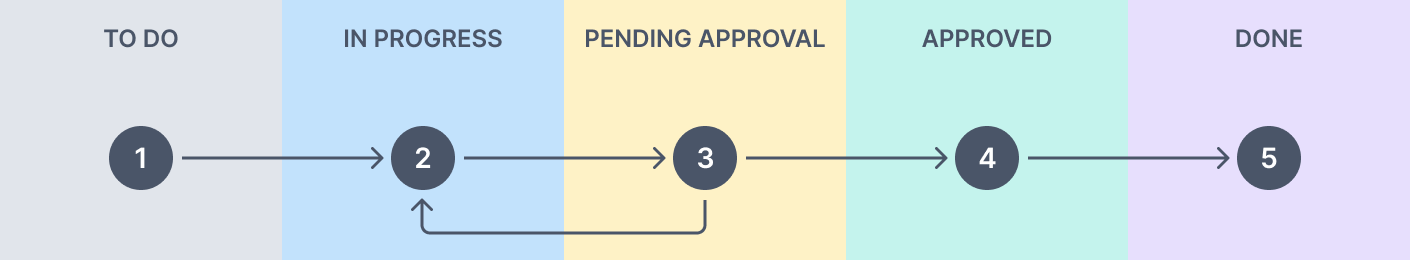
\includegraphics[width=\textwidth]{assets/working-packages/JiraWorkflow.png}
	\caption{5 steps of the Jira workflow}
\end{figure}
All the tasks would have to go from step 1 to step 5 in order to be considered as finished. Each step and the automation is as follows:
\begin{enumerate}
	\item All the tasks that have been selected for the sprint start at the first step, at the \emph{to-do} column.
	\item For each task, a new git branch has to be created with the name of the Jira task tag, for instance \texttt{HBL-185}\footnote{The \texttt{HBL} prefix is assigned when a new Jira project is created.}.
	      \\
	      When the branch is created and pushed to GitHub, Jira will move the task automatically to the \emph{in progress} column.
	      % TODO: Add Jira smart commits bibliography [21/03/2022]
	\item While in progress, each commit made is tracked in Jira. Additionally, Jira also supports \emph{smart commits} which are words prefixed with a hash (\#). With the smart commits, task properties can be changed. In this case, only the \texttt{\#time} has been used which increments the amount of time spent in each task. Tracking time has been useful to know more precisely how much time has been spent overall.
	\item Once the task is finished, a new pull request is made which triggers the continuous integration workflows set up at the GitHub repository. These workflows can also be watched by Jira and automate operations in function of the workflow result. If the task does not pass one of the workflows, the task is moved back to the \emph{in progress} tab. Alternatively, if the checks pass, it is moved to the \emph{approved} column.
	\item Finally, in order to be considered \emph{done}, the pull request of the task in question has to be merged. The merge will trigger another automated process which moves the task from \emph{approved} to \emph{done}.
\end{enumerate}
In order to stick to the process as much as possible, tasks moved to \emph{done}, should not be moved back. Instead, a new \emph{bug} type task was created which would start the process again.
\chapter{Requirements specifications}
\section{Introduction}
This chapter will cover the system requirements specification (\emph{SRS}) for the software being developed. The goal of this chapter is to establish the basis for what will be developed, taking into account user needs, functional and non-functional requirements.
\subsection{Purpose}
The application's objective is to provide a simple, scalable and powerful platform to handle gymnasium appointments. Gym owners will be able to create their gym zones and modify the constraints such as total capacity, available hours, closed days as needed. On the other side, gym clients will be able to book an appointment to the gyms they have access to.
\\[8pt]
Therefore, in a single application, gym owners and their workers will be able to control everything that happens inside the gym; while at the same time being able to apply changes and modifications as wanted.
\subsection{Definitions}
There are some definitions to be explained before moving to the next section:
\begin{enumerate}[label = -]
	\item \emph{Gym}. The gym will represent the company overall, not the infrastructure. Such infrastructure is called \emph{virtual gym}.
	\item \emph{Virtual gym}. A virtual gym will be the representation of a gymnasium in the application. A \emph{virtual gym} can have multiple \emph{gym zones}.
	\item \emph{Gym zone}. A gym zone will be the places where clients will book appointments.
	\item \emph{User}. The \emph{user} is the main person who uses the software. In this case, it is the owner and their workers.
	\item \emph{Template events}. Even though the class concept is explained in further sections, it is important to make a distinction between a \emph{class} and \emph{class template}, \emph{template events} or \emph{template events} (as they are named in the database). On the one hand, events will be assigned to a gym zone and scheduled. On the other hand, \emph{template events} will be used to schedule and link to a zone.
	\item \emph{Archiving} vs \emph{Deleting}. The purpose of archiving anything in the database means it will be stored but not visible. In order to edit it again, the archived element has to be \emph{recovered}. On the other hand, a deleted element will permanently be deleted from the database.
\end{enumerate}
\section{Overall description}
\subsection{Introduction}
This section provides a general explanation about the application, how it is intended to work, the different \emph{personas} to whom it is focused and a brief introduction to the software's functionalities.
\subsection{Product description}
The product will provide a rich interface for the gym owners and their coworkers in order to manage their gym. Managers will create virtual gyms, each of one with different constrains, which will be forwarded to their gym zones. Each gym zone will be of a certain type, for example, a cardio zone, a free-weight zone or even a powerlifting zone. Such and more characteristics will be determined by the workers or who is responsible for the creation of the zones. Once determined the capabilities of each zone, the clients will have the possibility to make their reservations.
\\[8pt]
This software is going to be interesting since it is mainly focused on the managing of appointments. There exist multiple manager systems, some are gym-focused yet there are few that provide an exclusive focus to managing the appointments. It is interesting to have an application that is that specific because most of the companies already have their client management system and other tools. The COVID has changed many things extremely fast and some gymnasiums have not been able to adapt fast enough. That is because using other management tools would mean to change the entire managing software of the company, in order words, starting from zero again. In the future, however, it would be nice to provide a client management system aswell, including subscriptions and so on.
\subsection{User needs}
After having briefly defined the application, two \emph{personas} can be identified: the owner or worker of the gym, and the client.
\\[8pt]
In the following sections, a brief explanation will be given about the functional requirements, yet such requirements will be explained more in depth in later sections.
\subsubsection{Owner or worker}
Such persona needs entire access to the management system, and it is the main user of it. For this persona, the following needs can be defined:
\begin{enumerate}[label = -]
	\item \emph{Ability to create virtual gyms and gym zones}. It is the main purpose of the application. It has to provide all the tools that are required to have an above average managing system.
	\item \emph{Modify virtual gyms and gym zones}. Constraints may change during time. Overall capacity may increase, more cardio machines may be added, and, with these changes, the gym zones will have to adapt to such real life modifications. There has to exist an interface that provides an easy and simple tool to control it.
	\item \emph{Ability to manage clients}. The income of the gym is based on the amount of clients they have, and such clients have to be subscribed into the system. However, the application is not a client management system. It purely focuses on the fact of appointments, yet the client still has to be registered in the application.
	\item \emph{Ability to manage appointments}. The workers have to be able to create, modify or delete the appointments at any time. This process has to be fast and simple, since it is more than usual to have cancellations, clients without reservation, and many more.
	\item \emph{Ability to manage guided events}. Some gym zones will be marked as a guided class zone. Therefore, a schedule will have to be set up for such zone in order to let the user know that.
\end{enumerate}
Furthermore, two user profiles have to be differentiated: the \emph{owner} and the \emph{worker}. The owner needs more control than the worker and some additional needs are\footnote{Some workers may also have access to such capabilities, depending on the permission they have recieved by the owner.}:
\begin{enumerate}[label = -]
	\item \emph{Ability to manage workers}. The owner has to be able to add, remove or update their workers. There must exist an interface that allows such control.
	\item \emph{Ability to manage the privileges of the workers}. In large gymnasium franchises, there may exist different types of workers, each with different tasks. For instance, some may only be able to manage guided sessions, others will manage the client subscriptions and so on. Therefore, a privilege system is required to define a hierarchy in the company.
	\item \emph{Ability to manage gym trainers}. It is important to know what trainers will be responsible for each guided class. For instance, some clients may prefer some trainers than others, when choosing a guided class.
\end{enumerate}
\subsubsection{Client}
The client has little interaction with the system. However, a management application for clients would be pointless if clients could not book their sessions. That is why it will exist another platform to provide access to the client. Such client, will have the following needs:
\begin{enumerate}[label = -]
	\item \emph{Ability to create, modify and delete appointments}. The clients will make the most use of the reservation system. There has to exist a simple and intuitive interface that allows the clients to interact with the system.
	\item \emph{Ability to visualise guided events}. In case the client prefers booking a place for a guided class, it should be able to visualise all the possible events for a day or week, for a zone.
\end{enumerate}
\section{Product functionalities}
The goal of this section is to explain how would the basic flow of the application be. From the owner arranging virtual gyms, the events and assigning the trainers; to the client being able to manage their appointments. By exemplifying the application behavior, it will be easier to determine the functional requirements of the software.
\subsection{Gym}
When registering, the owner will be required to enter the gym information and will be able to customise other information such as the gym contact data. Such settings will be common to all clients and workers, as they will be part of such gym.
\subsection{Virtual gym and gym zones}
The interface has to be intuitive both for the user and the client, while at the same time providing as much utility as possible. Before being able to create appointments, the client needs a place to create such appointments. Therefore, the first mission of the owner is to define each zone. A gym company may have one or more virtual gyms. As stated before, a virtual gym is the representation of the gym infrastructure in the system. Each virtual gym will have different characteristics and information as: the gym location, the total capacity, the opening and closing hours and much more. This virtual gyms can be modified as they may change time to time. If ever needed, the fact of deleting the different virtual gyms will also be possible.
\\[8pt]
Once the virtual gym has been set up, it can have gym zones. Each gym zone will also have its characteristics, most of them similar to the virtual gym ones. However, there is a characteristic that is important to mention: the \emph{type} of the gym zone. Each zone is required a type since some zones may be suitable for events and some not. Such types will be predefined, however the user will have the ability to create their own types. Nonetheless, there will still be the need of distinction between class zones and non-class zones.
\subsection{Events, trainers and workers}
After having defined the structure of the gym, the owner or the workers of the gym can create and schedule events for the different gym zones. Events can not be overlapped in the same zone, yet some events can be scheduled at the same time in different zones. Furthermore, the same class can be done in multiples zones, with different trainers.
\\[8pt]
In order to keep such consistency, the gym owners will create \emph{template events}, which will have specific characteristics. Each template class will be unique, and it will be used to create \emph{events}. In short, the client will create an appointment to a class, which will be a scheduled template class. Nonetheless, appointments will also be required for non-class gym zones, as it is needed to know how many users will access such zone in a certain time. With the explained relation, owners and workers will not have the need to create a class with all the details every single time, rather simply scheduling already created template events.
\\[8pt]
Additionally, a trainer manager system is required. However, a trainer it is a worker as well, only it does not interact with the application. Hence, in the same management view, the owner, and if any worker is allowed to, will be able to create trainers and workers.
\subsection{Clients}
Before continuing, the system still lacks of the main income of the gymnasium: the client. As detailed before, the goal of this application is not to provide a client management system, though it could be a functionality to be implemented in the future. Therefore, the client will also be related to the gym entity.
\\[8pt]
There has to be, definitely, a small client management. However, this management does not need to know about all the information it is kept about the user in the gym. It will only need:
\begin{enumerate}[label = -]
	\item Personal information such as the name, last name and so on. It should include an email to log in to the software.
\end{enumerate}
That is it. From there, the client will have access to another view of the application in which they will be able to make the reservations.
\subsection{Creating appointments}
When the client has been able to connect to the platform, they will be able to visualise the virtual gyms of the gym they belong to. There, the client will see the availability of the different gym zones, the events offered in that zone and other relevant information. From there, they will create their appointments which will be persisted in the system.
\\[8pt]
After the appointment has been made, the client will be able to modify it and remove it, without the need of any explanation.
\section{Functional requirements}
\subsection{Introduction}
In this section, the above described requirements will be explained more in depth. The functional requirements are defined as the core functionalities of the system. All requirements exposed in the section are considered essentials and the system would be considered incomplete if it did not satisfy such requisites.
\\[8pt]
The requisites will be exposed with their code name and a number (as \emph{FR-1}), their priority and a brief description. Three levels of priority have been defined:
\begin{enumerate}[label = \arabic{*}.]
	\item \textbf{High priority (3)}. Such requisites must be fulfilled by the application in order to provide a proper user experience.
	\item \textbf{Medium priority (2)}. Such requisites should be fulfilled by the application in order to provide an above average user experience.
	\item \textbf{Low priority (1)}. Such requisites would provide an excellent user experience, yet they are not mandatory.
\end{enumerate}
Furthermore, the overall application will be separated in three different front end applications:
\begin{enumerate}[label = \textbf{\arabic{*}.}]
	\item \textbf{Landing app}. Application which contains the landing application of the product.
	\item \textbf{Core app}. Main application of the product, where the user does most of the work.
	\item \textbf{Appointments app}. Application used by the gym client in order to book their appointments.
\end{enumerate}
\subsection{Landing app - Product information}
The application must have a landing page in which the potential user can find the different features offered by the application.
\begin{enumerate}[label = -]
	\item \textbf{FR-1 (3)}. The user needs to know the different features of the product in a single page.
	\item \textbf{FR-2 (3)}. The user needs to be able to be redirected to the register and login page, from the landing page. Such page is the core page.
	\item \textbf{FR-3 (2)}. The user needs to be able to find a contact page in the landing page and ask for the desired information by providing personal information.
	\item \textbf{FR-4 (3)}. The user needs to find information about the data privacy. No personal data and information is intended to be sold, nor shared.
\end{enumerate}
\subsection{Core app - User registration}
The user, in this case the owner, has to be able to register. In the beginning, the application will be completely free, so the gym owners will have complete access only by registering. A future implementation would be to provide additional features only to the users with a subscription.
\begin{enumerate}[label = -]
	\item \textbf{FR-5 (3)}. The user has to provide personal information in order to register.
	\item \textbf{FR-6 (3)}. The user has to provide information about the gym in order to register.
	\item \textbf{FR-7 (3)}. The user has to provide an email and a password to access the application (log in).
	\item \textbf{FR-8 (3)}. The user needs to be able to see how their data is kept (personal data privacy).
	\item \textbf{FR-9 (1)}. The user should see the information for the different premium and free plans.
	\item \textbf{FR-10 (1)}. The user could have a free trial for the premium features.
\end{enumerate}
\subsection{Core app - Home page}
In the home page view, the user will manage their virtual gyms and gym zones. Furthermore, it will be able to create, update and remove the template events which will be then linked to gym zones schedule.
\subsubsection{Virtual gyms}
The user will enter the home page and will see the list of their virtual gyms. If no virtual gym has been created, they will be asked if they want to create a virtual gym (which will be optional). From the same view, they will be able to create, modify and archive the different virtual gyms, aside from accessing the gym zones of that virtual gym.
\begin{enumerate}[label = -]
	\item \textbf{FR-11 (3)}. The view has to display a list or a grid with the different virtual gyms of the user.
	\item \textbf{FR-12 (3)}. Each virtual gym item has to provide an option to visualise and update all the information of that virtual gym. This means changing both the virtual gym \emph{metadata}, and the virtual gym constraints.
	\item \textbf{FR-13 (3)}. The user has to access the virtual gym view by clicking on a virtual gym.
	\item \textbf{FR-14 (3)}. The user has to access the gym zones view by clicking on a virtual gym.
	\item \textbf{FR-15 (2)}. The user has to be able to search for a virtual gym by its name.
	\item \textbf{FR-16 (1)}. Each virtual gym item has to provide an option to archive that virtual gym (and, consequentially, all the gym zones).
	\item \textbf{FR-17 (1)}. There virtual gym list has to provide an option to programmatically sort the virtual gyms (e.g. by ascending or descending capacity).
	\item \textbf{FR-18 (1)}. There virtual gym list has to provide an option to manually sort the virtual gyms.
\end{enumerate}
\subsubsection{Gym zones}
Once a virtual gym has been created and the user has clicked on the card representing it, the user will be redirected to another view in which the zones of the gym will be displayed. Similarly, as in the virtual gyms view, if the user has not created any gym zone, they will be prompted to do so, if wanted.
\begin{enumerate}[label = -]
	\item \textbf{FR-19 (3)}. The view has to display a list or a grid with the different gym zones of the selected virtual gym.
	\item \textbf{FR-20 (3)}. Each gym zone has to provide an option to visualise and update all the information of that gym zone. This means changing both the gym zone \emph{metadata}, and the gym zone constraints.
	\item \textbf{FR-21 (3)}. The view has to display which zones are class type and wich not.
	\item \textbf{FR-22 (2)}. The user has to see the gym zone view by clicking on it.
	\item \textbf{FR-23 (1)}. Each gym zone has to provide an option to archive the zone.
\end{enumerate}
\subsubsection{Class gym zone schedule}
When the user has created a class gym zone, that zone will have a schedule (or a calendar). Inside this view, the user will be able to see the schedule or calendar from the selected gym zone.
\begin{enumerate}[label = -]
	\item \textbf{FR-24 (3)}. The view has to provide an option to visualise the current schedule of events.
	\item \textbf{FR-25 (3)}. From the calendar, the user has to be able to create a guided session by linking a template class to it. Such \emph{scheduled event} must include: a start and end time, the trainer which will be the guide, a maxiumum capacity and other information.
	\item \textbf{FR-26 (3)}. From the calendar, the user has to be able to create an event.
	\item \textbf{FR-27 (2)}. From the calendar, the user has to be able to see future scheduled events.
	\item \textbf{FR-28 (1)}. From the calendar, the user has to be able to see past scheduled events.
	\item \textbf{FR-29 (1)}. The user has to be able to create guided sessions which are repeated when wanted, from the chosen interval.
	\item \textbf{FR-30 (1)}. After creating a new class on a gym zone, the application has to \emph{recommend} a trainer for that class.
\end{enumerate}
\subsection{Core app - Events page}
Even though this view is simple, it is important to separate the schedule view of a gym zone from the template events. The current view will only provide the necessary tools to create, edit, delete or archive the different event templates.
\begin{enumerate}[label = -]
	\item \textbf{FR-31 (3)}. The user has to be able to see the gym list of event types.
	\item \textbf{FR-32 (3)}. There has to be an option in the menu which allows the user to create, update and delete event types.
	\item \textbf{FR-33 (3)}. The user has to be able to see the gym list of template events.
	\item \textbf{FR-34 (3)}. There has to be an option in the menu which allows the user to create, update and delete template events.
	\item \textbf{FR-35 (2)}. The user has to be able to archive the event types.
	\item \textbf{FR-36 (1)}. The user has to be able to archive template events.
\end{enumerate}
\subsection{Core app - Workers page}
This view has to allow the user to manage the workers of the gym enterprise and set the different permissions.
\begin{enumerate}[label = -]
	\item \textbf{FR-37 (3)}. The user has to be able to create a new worker, providing personal information and credentials for such worker to user the app. Furthermore, it has to allow the user to set the permissions for that worker.
	\item \textbf{FR-38 (3)}. The same view has to provide an option to update the permissions and the personal information of the worker.
	\item \textbf{FR-39 (3)}. The view has to provide a table to list all the workers.
	\item \textbf{FR-40 (1)}. The user has to be able to set the working hours of each worker.
	\item \textbf{FR-41 (1)}. The view has to provide an input to search the by name, last name or other characteristics the different workers.
\end{enumerate}
\subsection{Core app - Trainers page}
This view has to allow the user to manage the trainers of the gym enterprise.
\begin{enumerate}[label = -]
	\item \textbf{FR-42 (3)}. The user has to be able to create a new trainer, providing personal information and credentials for such worker to user the app.
	\item \textbf{FR-43 (3)}. The same view has to provide an option to update the trainer personal information.
	\item \textbf{FR-44 (3)}. The view has to provide a table list all the trainers.
	\item \textbf{FR-45 (1)}. The user has to be able to set the working hours of each trainer.
	\item \textbf{FR-46 (1)}. The view has to provide an input to search the by name, last name or other characteristics the different trainers.
\end{enumerate}
\subsection{Core app - Clients page}
This view has to allow the user to manage the clients of the gym enterprise.
\begin{enumerate}[label = -]
	\item \textbf{FR-47 (3)}. The user has to be able to create a new client, providing personal information and credentials for such worker to user the app. Alternatively, the client can register himself (\textbf{FR-65}) with a gym code.
	\item \textbf{FR-48 (3)}. The same view has to provide an option to update the client personal information.
	\item \textbf{FR-49 (3)}. The view has to provide a table list all the clients.
	\item \textbf{FR-50 (1)}. The view has to provide an input to search the by name, last name or other characteristics the different clients.
\end{enumerate}
\subsection{Core app - Settings page}
This view has to provide enough settings to customizer the behavior of the behavior and the gym information.
\begin{enumerate}[label = -]
	\item \textbf{FR-51 (3)}. The view has to allow the user to log out.
	\item \textbf{FR-52 (3)}. As an owner, the settings menu has to allow the user to change the gym name and gym characteristics.
	\item \textbf{FR-53 (3)}. As an owner or worker, the settings page has to allow the user to change their personal information.
	\item \textbf{FR-54 (3)}. As an owner or worker, the settings page has to allow the user to change their password.
	\item \textbf{FR-55 (1)}. The settings menu has to provide an option to change the application theme (light and dark) and persist it.
	\item \textbf{FR-56 (1)}. The settings menu has to provide an option to customise the main colours of the user interface.
\end{enumerate}
\subsection{Core app - Analysis page}
The goal of this view is to provide some metrics to \emph{what is happening at the gym}. However, \textbf{as it is not the main purpose of the application}, all the requirements from each will be marked with \emph{low priority}.
\begin{enumerate}[label = -]
	\item \textbf{FR-57 (1)}. The view has to provide a select option to choose what virtual gym wants to be analised.
	\item \textbf{FR-58 (1)}. After having selected a virtual gym, the view has to display in which intervals the virtual gym is most crowded at the current date.
	\item \textbf{FR-59 (1)}. After having selected a virtual gym, the view has to display in which intervals the virtual gym is most crowded during an interval.
	\item \textbf{FR-61 (1)}. After having selected a virtual gym, the view has to display what events will have more clients during an interval.
	\item \textbf{FR-62 (1)}. After having selected a virtual gym, the view has to display what events will have more clients during at the current date.
	\item \textbf{FR-63 (1)}. After having selected a virtual gym, the view has to provide a filter to check what gym zones are more crowded during an interval.
	\item \textbf{FR-64 (1)}. After having selected a virtual gym, the view has to provide a filter to check what gym zones are more crowded at the current date.
\end{enumerate}
\subsection{Client app}
The client application will reuse most of the content from the Core application. However, as it is a client, all the functionalities of modifying and deleting will no appear, as the client does not have access to such views.
\begin{enumerate}[label = -]
	\item \textbf{FR-65 (3)}. The client has to provide personal information and a gym code in order to register.
	\item \textbf{FR-66 (3)}. The client has to provide an email and password to access the application (log in).
	\item \textbf{FR-67 (3)}. The home page has to display a list or a grid with the different virtual gyms of the gym they are subscribed.
	\item \textbf{FR-68 (3)}. On clicking any virtual gym, the home view has to display the gym zones of the selected virtual gym.
	\item \textbf{FR-69 (3)}. The calendar should display the scheduled events, week by week.
	\item \textbf{FR-70 (2)}. On clicking a scheduled event, the client will be able to book a place, if the event is not full.
	\item \textbf{FR-71 (3)}. If the user clicks on a non-class gym zone, a form has to be shown to choose the interval in which they want to make the appointment. This includes the date of the appointment, the duration and the starting hour.
	\item \textbf{FR-72 (3)}. On selecting a date and a duration, the server has to return what available starting hours there are. If there is no capacity for such selections, the user will not be able to create the appointment.
\end{enumerate}
\subsection{Client app - Settings page}
The personal information, which is nearly the settings page for the client, has to display most of their information. Additionally, it can show some user stats \emph{for the geeks}.
\begin{enumerate}[label = -]
	\item \textbf{FR-73 (3)}. The view has to allow the user to log out.
	\item \textbf{FR-74 (3)}. The view has to allow the client to change their personal information.
	\item \textbf{FR-75 (3)}. The view has to allow the client to change their password.
	\item \textbf{FR-76 (3)}. The view has to display a list with all the upcoming appointments of the user.
	\item \textbf{FR-77 (1)}. If wanted, the user has to be able to see a list with all the past appointments.
	\item \textbf{FR-78 (1)}. The settings menu has to provide an option to change the application theme (light and dark) and persist it.
	\item \textbf{FR-79 (1)}. The view has to display an analytics table to see which days have they accessed a virtual gym.
\end{enumerate}
\section{Non-functional requirements}
A non-functional requirement is a requirement that defines system attributes such as security, reliability, maintainability, scalability and usability. Therefore, such requisites do not describe information to keep nor functionalities to implement, rather characteristics of such functionalities. In the system, the following non-functional requirements can be defined:
\begin{enumerate}[label = -]
	\item \textbf{NFR-1 (3)}. The system has to provide a secure authentication method.
	\item \textbf{NFR-2 (2)}. The application has to provide different authentication methods in order to differentiate the gym owner, the gym worker and the gym client.
	\item \textbf{NFR-3 (2)}. The landing and client web applications must provide a responsive interface, so that the application can be seen both in small and large screens.
	\item \textbf{NFR-4 (1)}. The core application has to provide a responsive interface up to a point. In smaller screens such as phones, some functionalities would not be easy to implement nor to use.
	\item \textbf{NFR-5 (2)}. The three web applications have to provide an accessible and semantic HTML structure.
\end{enumerate}
\section{Requirements dependency matrix}
Due to the large quantity of requirements that have been determined for the development of the project, and due to the low relationship between them, the dependencies will be shown individually, in order to avoid displaying a nearly empty table. Using the following notation, the result is more consise and can be understood better.
\\[8pt]
Each dependency will use the following format: \textbf{[FR-1, FR-2, FR-3] \texttt{->} [FR-4, FR-5]}. It states that the functional requirements 1, 2 and 3 depend on the 4 and the 5.
\\[8pt]
\textbf{[FR-11, FR-13, FR-14, FR-16, FR-17, FR-18] \texttt{->} [FR-12]}. In order to visualise, edit or delete a virtual gym, such virtual gym has had to be created previously.
\\[8pt]
\textbf{[FR-19, FR-20, FR-21, FR-22, FR-23] \texttt{->} [FR-12]}. The gym zones are required to exist inside a virtual gym. If such virtual gym has not been created, the user can not visualise, edit or delete the gym zone.
\\[8pt]
\textbf{[FR-19, FR-21, FR-22, FR-23] \texttt{->} [FR-20]}. In order to visualise, edit or delete a gym zone, such gym zone has had to be created previously.
\\[8pt]
\textbf{[FR-24, FR-25, FR-26, FR-27, FR-28, FR-29, FR-30] \texttt{->} [FR-20]}. A calendar is required to exist inside a gym zone. If such gym zone has not been created, the user can not visualise, edit or delete the events of the calendar.
\\[8pt]
\textbf{[FR-31, FR-35] \texttt{->} [FR-32]}. In order to visualise, edit or delete an event type, such event type has had to be created previously.
\\[8pt]
\textbf{[FR-33, FR-36] \texttt{->} [FR-36]}. In order to visualise, edit or delete an event template, such event template has had to be created previously.
\\[8pt]
\textbf{[FR-38, FR-39, FR-40, FR-41] \texttt{->} [FR-27]}. In order to visualise, edit or delete a worker, such worker has had to be created previously.
\\[8pt]
\textbf{[FR-43, FR-44, FR-45, FR-46] \texttt{->} [FR-42]}. In order to visualise, edit or delete a trainer, such trainer has had to be created previously.
\\[8pt]
\textbf{[FR-48, FR-49, FR-50, FR-51] \texttt{->} [FR-47]}. In order to visualise, edit or delete a client, such client has had to be created or registered previously.
\\[8pt]
\textbf{[FR-66, FR-67, FR-68, FR-69, FR-70, FR-71, FR-72] \texttt{->} [FR-65]}. In order to interact with the application, the client must be registered previously.
\chapter{Planning}
This chapter will cover the planning of the project. After having defined the requirements and the matrix of dependencies of such requirements, working packages will be defined, which will ensure an organized development using tasks.
\section{Working packages}
\label{working-packages}
Each's table corresponds to one of the working packages. Since the \emph{Development} branch of the working packages tree the most extensive, its tables are explained after the \emph{Testing} branch, and so are the package numbers.
\begin{figure}[H]
	\centering
	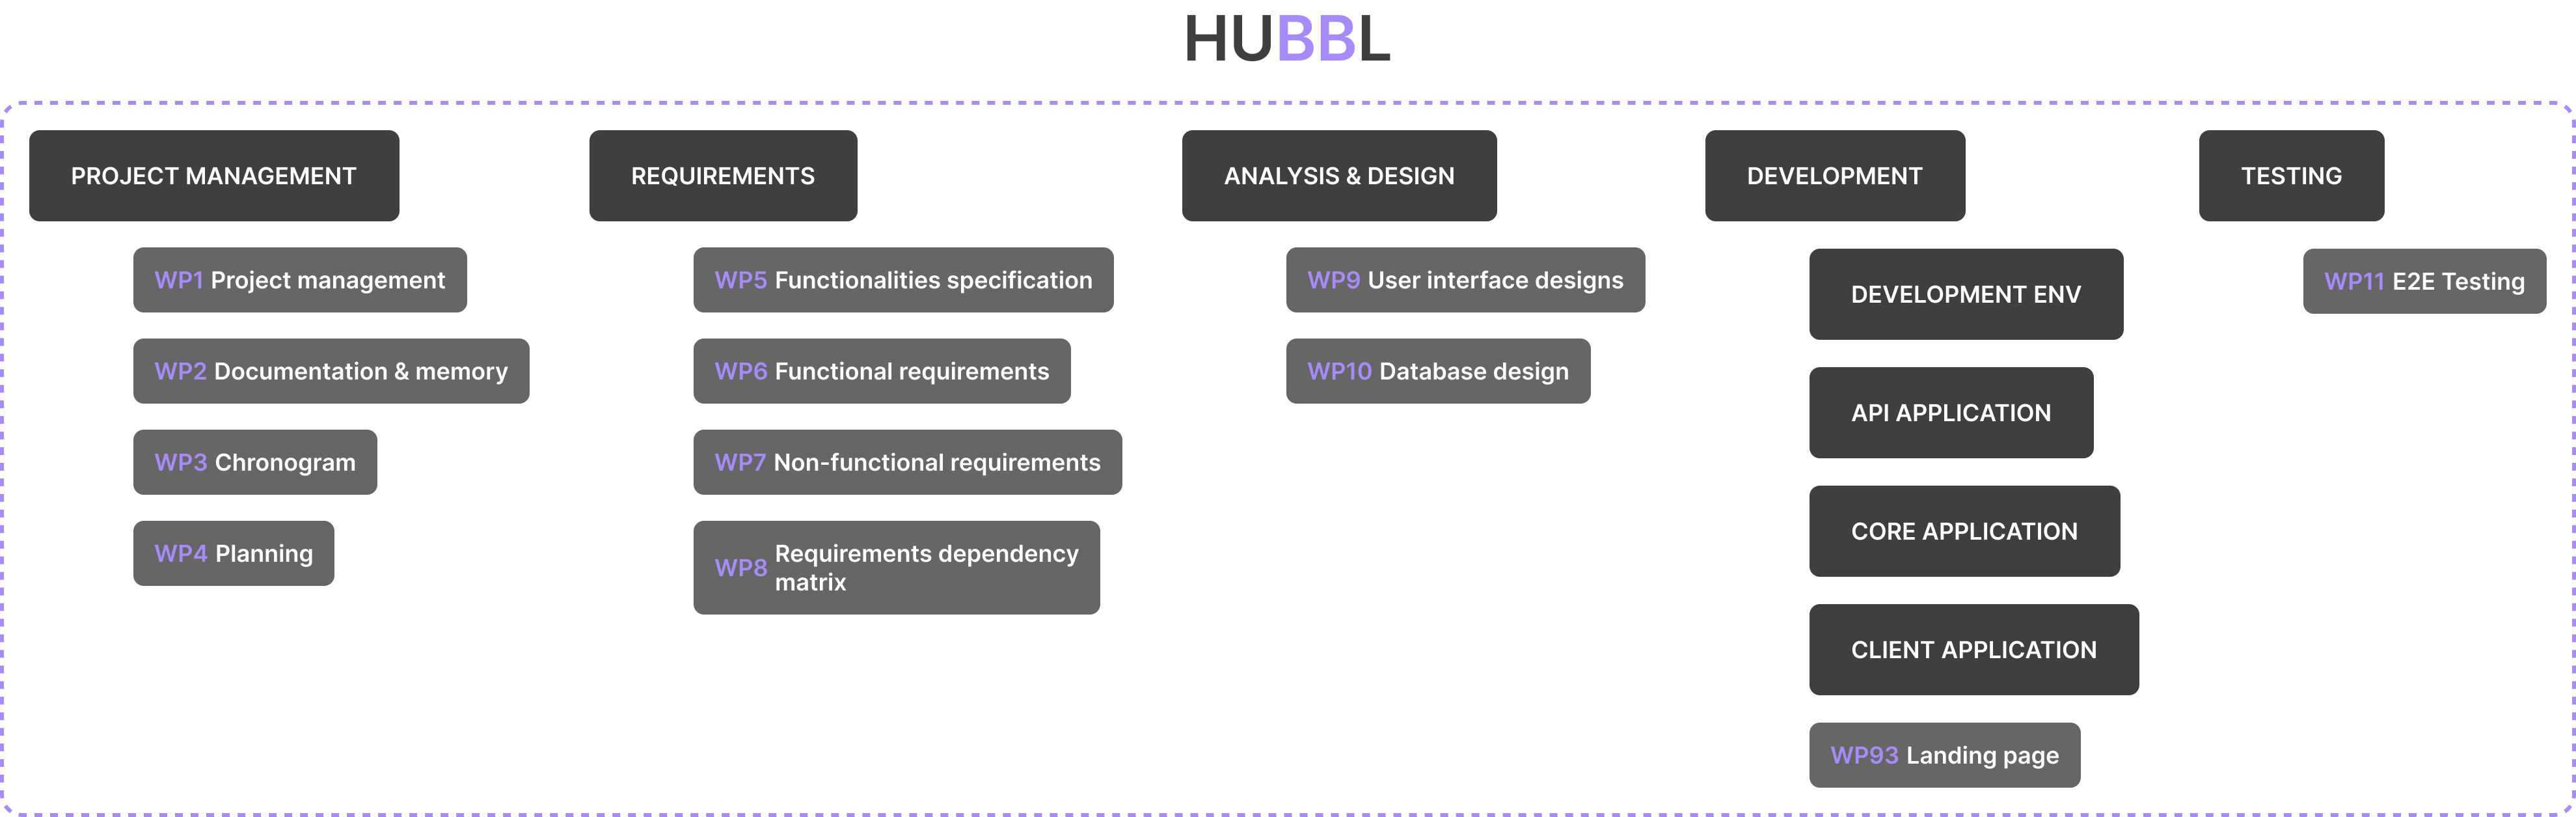
\includegraphics[width=\textwidth]{assets/working-packages/All.png}
	\caption{Structure of the working packages at the root level}
\end{figure}
The image above shows how the working packages have been organized. Each column represents a module, which are:
\begin{enumerate}[label = -]
	\item Project management.
	\item Requirements.
	\item Analysis and design.
	\item Development.
	\item Testing.
\end{enumerate}
Since the development branch is very extensive, each project has been extracted in smaller working packages.
\subsection{Project management}
The \emph{project management} branch contains all the working packages that are related any task that involves the specification of how the project will be managed in order to be successful.
\\[8pt]
\begin{tabularx}{\textwidth}{| l | X |}
	\hline
	\rowcolor{rowColor}
	{\semibf Package name}   & {\semibf WP1}: Project management             \\
	\hline
	{\semibf Description}    & Working package description.                  \\
	\hline
	\rowcolor{rowColor}
	{\semibf Estimated time} & 8h                                            \\
	\hline
	{\semibf Tasks}          & {\semibf T1}: Project document writing.
	\newline {\semibf T2}: Project document review.                          \\
	\hline
	\rowcolor{rowColor}
	{\semibf Results}        & Project document to be submitted to the jury. \\
	\hline
\end{tabularx}
\captionof{table}{Package one's table - Project management}
\vspace*{16pt}
\begin{tabularx}{\textwidth}{| l | X |}
	\hline
	\rowcolor{rowColor}
	{\semibf Package name}   & {\semibf WP2}: Documentation and memory            \\
	\hline
	{\semibf Description}    & Wording of some chapters of the memory.            \\
	\hline
	\rowcolor{rowColor}
	{\semibf Estimated time} & 8h                                                 \\
	\hline
	{\semibf Tasks}          & {\semibf T1}: Wording of the project introduction.
	\newline {\semibf T2}: Wording of the requirements.
	\newline {\semibf T3}: Wording of the analysis and design.
	\newline {\semibf T4}: Wording of the studies and decisions.
	\newline {\semibf T5}: Wording of the project development.                    \\
	\hline
	\rowcolor{rowColor}
	{\semibf Results}        & Project document to be submitted to the jury.      \\
	\hline
\end{tabularx}
\captionof{table}{Package two's table - Documentation and memory}
\vspace*{16pt}
\begin{tabularx}{\textwidth}{| l | X |}
	\hline
	\rowcolor{rowColor}
	{\semibf Package name}   & {\semibf WP3}: Chronogram                                  \\
	\hline
	{\semibf Description}    & Define the working chronogram for the project development. \\
	\hline
	\rowcolor{rowColor}
	{\semibf Estimated time} & 4h                                                         \\
	\hline
	{\semibf Tasks}          & {\semibf T1}: Temporal planning of the working packages.   \\
	\hline
	\rowcolor{rowColor}
	{\semibf Results}        & Gantt's project diagram.                                   \\
	\hline
\end{tabularx}
\captionof{table}{Package three's table - Chronogram}
\vspace*{16pt}
\begin{tabularx}{\textwidth}{| l | X |}
	\hline
	\rowcolor{rowColor}
	{\semibf Package name}   & {\semibf WP4}: Planning                         \\
	\hline
	{\semibf Description}    & Structure the working packages.                 \\
	\hline
	\rowcolor{rowColor}
	{\semibf Estimated time} & 4h                                              \\
	\hline
	{\semibf Tasks}          & {\semibf T1}: Planning of the working packages. \\
	\hline
	\rowcolor{rowColor}
	{\semibf Results}        & Chapter 6 of the memory document.               \\
	\hline
\end{tabularx}
\captionof{table}{Package four's table - Planning}
\vspace*{16pt}
\begin{tabularx}{\textwidth}{| l | X |}
	\hline
	\rowcolor{rowColor}
	{\semibf Package name}   & {\semibf WP5}: Functionalities specification        \\
	\hline
	{\semibf Description}    & Analysis of the functionalities of the application. \\
	\hline
	\rowcolor{rowColor}
	{\semibf Estimated time} & 8h                                                  \\
	\hline
	{\semibf Tasks}          & {\semibf T1}: Users identification.
	\newline {\semibf T2}: Define user needs (owner/worker and client).
	\newline {\semibf T3}: Define product functionalities                          \\
	\hline
	\rowcolor{rowColor}
	{\semibf Results}        & Sections 5.2 and 5.3 of the memory document.        \\
	\hline
\end{tabularx}
\captionof{table}{Package five's table - Functionalities specification}
\subsection{Requirements}
The \emph{requirements} branch contains all the tasks that are related with the analysis and definition of all the requirements and functionalities of each application.
\\[8pt]
\begin{tabularx}{\textwidth}{| l | X |}
	\hline
	\rowcolor{rowColor}
	{\semibf Package name}   & {\semibf WP6}: Functional requirements                                     \\
	\hline
	{\semibf Description}    & Analysis and definition of the functional requirements of the application. \\
	\hline
	\rowcolor{rowColor}
	{\semibf Estimated time} & 12h                                                                        \\
	\hline
	{\semibf Tasks}          & {\semibf T1}: Use case diagram.
	\newline {\semibf T2}: Functional requirements' specification for the \textit{core} application.
	\newline {\semibf T3}: Functional requirements' specification for the \textit{client} application.
	\newline {\semibf T4}: Functional requirements' specification for the \textit{landing} application.
	\newline {\semibf T5}: Functional requirements review and make changes if needed.                     \\
	\hline
	\rowcolor{rowColor}
	{\semibf Results}        & Section 5.4 of the memory document.                                        \\
	\hline
\end{tabularx}
\captionof{table}{Package six's table - Functional requirements}
\vspace*{16pt}
\begin{tabularx}{\textwidth}{| l | X |}
	\hline
	\rowcolor{rowColor}
	{\semibf Package name}   & {\semibf WP7}: Non-functional requirements                                     \\
	\hline
	{\semibf Description}    & Analysis and definition of the non-functional requirements of the application. \\
	\hline
	\rowcolor{rowColor}
	{\semibf Estimated time} & 4h                                                                             \\
	\hline
	{\semibf Tasks}          & {\semibf T1}: Initial non-functional requirements' specification.
	\newline {\semibf T2}: Non-functional requirements review and make changes if needed.                     \\
	\hline
	\rowcolor{rowColor}
	{\semibf Results}        & Section 5.5 of the memory document.                                            \\
	\hline
\end{tabularx}
\captionof{table}{Package seven's table - Non-functional requirements}
\vspace*{16pt}
\begin{tabularx}{\textwidth}{| l | X |}
	\hline
	\rowcolor{rowColor}
	{\semibf Package name}   & {\semibf WP8}: Requirements dependency matrix          \\
	\hline
	{\semibf Description}    & Definition of the requirements' dependency matrix.     \\
	\hline
	\rowcolor{rowColor}
	{\semibf Estimated time} & 4h                                                     \\
	\hline
	{\semibf Tasks}          & {\semibf T1}: Matrix dependency specification once the
	functional and non-functional requirements have been specified.                   \\
	\hline
	\rowcolor{rowColor}
	{\semibf Results}        & Section 5.6 of the memory document.                    \\
	\hline
\end{tabularx}
\captionof{table}{Package eight's table - Requirements dependency matrix}
\subsection{Analysis and design}
The \emph{analysis and design} branch contains all the working packages that are related with the design and analysis of the system interface and architecture.
\\[8pt]
\begin{tabularx}{\textwidth}{| l | X |}
	\hline
	\rowcolor{rowColor}
	{\semibf Package name}   & {\semibf WP9}: User interface designs                                 \\
	\hline
	{\semibf Description}    & Definition of the requirements' dependency matrix.                    \\
	\hline
	\rowcolor{rowColor}
	{\semibf Estimated time} & 96h                                                                   \\
	\hline
	{\semibf Tasks}          & {\semibf T1}: Design system specification.
	\newline {\semibf T2}: Prototype most of the user interfaces.
	\newline {\semibf T3}: Design review. Ensure it satisfies the requirements previously specified. \\
	\hline
	\rowcolor{rowColor}
	{\semibf Results}        & User interface prototypes which provide a vague view of the
	application's look and feel.                                                                     \\
	\hline
\end{tabularx}
\captionof{table}{Package nine's table - User interfaces designs}
\vspace*{16pt}
\begin{tabularx}{\textwidth}{| l | X |}
	\hline
	\rowcolor{rowColor}
	{\semibf Package name}   & {\semibf WP10}: Database design                                       \\
	\hline
	{\semibf Description}    & Definition of the application's database.                             \\
	\hline
	\rowcolor{rowColor}
	{\semibf Estimated time} & 4h                                                                    \\
	\hline
	{\semibf Tasks}          & {\semibf T1}: Design of the applications' database structure.
	\newline {\semibf T2}: Schema and structure review.
	\newline {\semibf T3}: Analysis of the database structure using PostgreSQL.                      \\
	\hline
	\rowcolor{rowColor}
	{\semibf Results}        & Database structure in which the application's data will be persisted. \\
	\hline
\end{tabularx}
\captionof{table}{Package ten - Database design}
\subsection{Testing}
The \emph{testing} branch contains the working package that is related with the testing of the application.
\\[8pt]
\begin{tabularx}{\textwidth}{| l | X |}
	\hline
	\rowcolor{rowColor}
	{\semibf Package name}   & {\semibf WP11}: E2e testing                                              \\
	\hline
	{\semibf Description}    & End-to-end testing implementation for the applications.                  \\
	\hline
	\rowcolor{rowColor}
	{\semibf Estimated time} & 4h                                                                       \\
	\hline
	{\semibf Tasks}          & {\semibf T1}: \emph{API} aplication e2e testing.
	\newline {\semibf T2}: \emph{Core} application e2e testing.
	\newline {\semibf T3}: \emph{Client} application e2e testing.
	\newline {\semibf T4}: \emph{Landing} application e2e testing.                                      \\
	\hline
	\rowcolor{rowColor}
	{\semibf Results}        & End-to-end tests which ensure the correct behaviour of each application,
	and that any futher new features and updates do not break the application.                          \\
	\hline
\end{tabularx}
\captionof{table}{Package eleven's table - E2e testing}
\subsection{Development}
\label{working-packages-development}
% TODO: Add methodology reference
The \emph{development} branch is probably the most extensive, as it is the most important part of the project. The branch consists of 73 working packages in total. Nevertheless, most of the packages follow the same structure. For instance, as it is seen in the \nameref{working-packages-api}, each web service package follows the same structure: a working package to create an entity, another one to update it, a third one to delete it, and a final one to fetch the entity. The structure is the same for each web service, which easily increases the number of working packages.
\subsubsection{Development env}
The first group that is in the \emph{development} branch is the \emph{development env} (or \emph{development environment}). This part is as important as any other application, since it will define the structure of the project. Furthermore, the continuous integration has to be set up. Using the Nx build system, such feature becomes extremely simple and scalable. One of the options it offers is to run a command to as many projects as wanted. Not only so, that you can run the commands to the affected projects. Such feature reduces even more the CI execution time.
\begin{figure}[H]
	\centering
	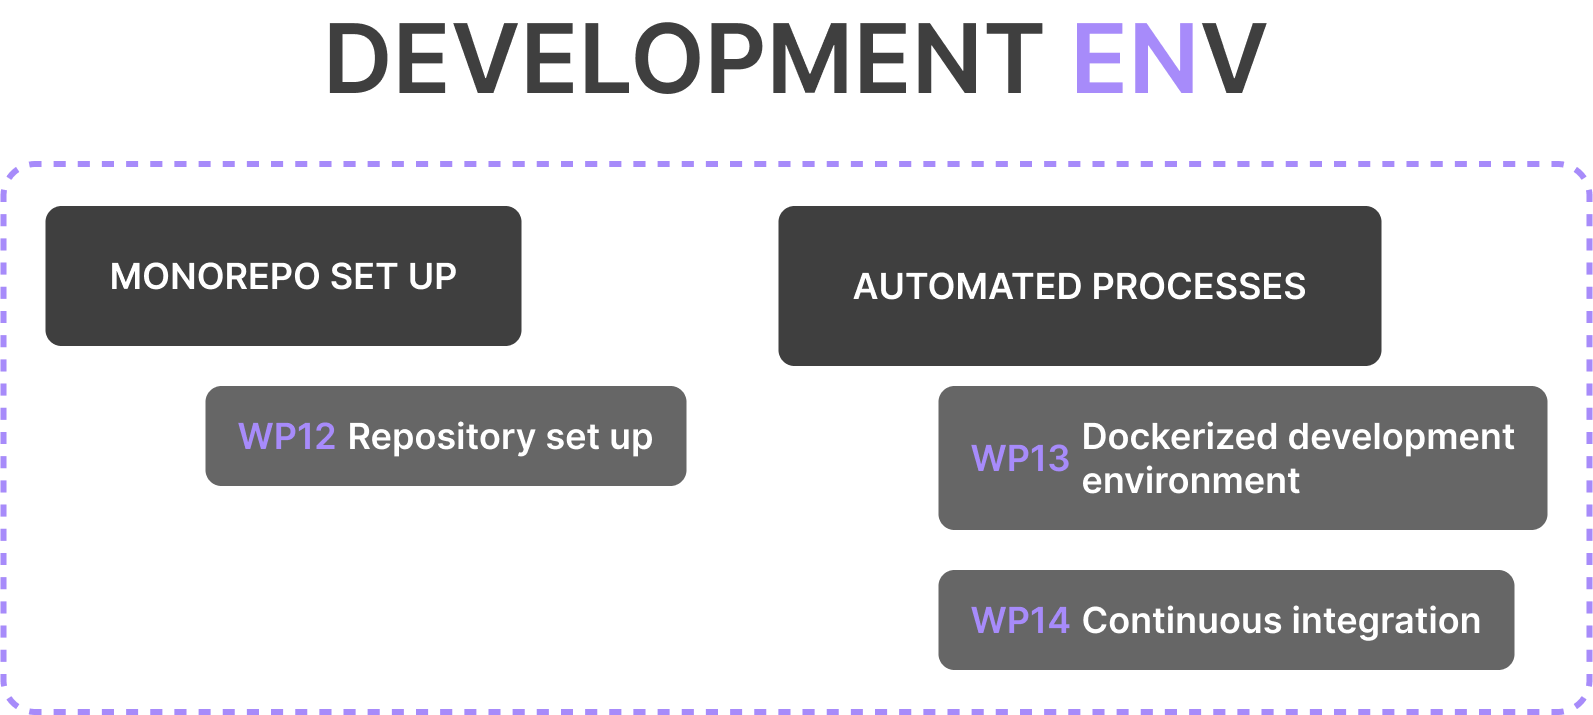
\includegraphics[width=\textwidth]{assets/working-packages/DevEnv.png}
	\caption{Api application working packages diagram}
\end{figure}
The \emph{development environment} group is composed of the following working packages:
\\[8pt]
% region PLANNING_TABLES
\begin{tabularx}{\textwidth}{| l | X |}
	\hline
	\rowcolor{rowColor}
	{\semibf Package name}   & {\semibf WP12}: Repository set up                                 \\
	\hline
	{\semibf Description}    & Prepare the Nx monorepo.                                          \\
	\hline
	\rowcolor{rowColor}
	{\semibf Estimated time} & 2h                                                                \\
	\hline
	{\semibf Tasks}          & {\semibf T1}: Generate an \texttt{nx-workspace} ready to develop. \\
	\hline
	\rowcolor{rowColor}
	{\semibf Results}        & Initial structure of the monorepo.                                \\
	\hline
\end{tabularx}
\captionof{table}{Package twelve's table - Repository set up}
\vspace*{16pt}
\begin{tabularx}{\textwidth}{| l | X |}
	\hline
	\rowcolor{rowColor}
	{\semibf Package name}   & {\semibf WP13}: Dockerized development environment.                \\
	\hline
	{\semibf Description}    & Dockerize the database, the test database and the API application. \\
	\hline
	\rowcolor{rowColor}
	{\semibf Estimated time} & 2h                                                                 \\
	\hline
	{\semibf Tasks}          & {\semibf T1}: Dockerize the main database and the test database.
	\newline {\semibf T2}: Dockerize the API application using a NodeJS image.                    \\
	\hline
	\rowcolor{rowColor}
	{\semibf Results}        & The dockerization of the databases and the REST API.               \\
	\hline
\end{tabularx}
\captionof{table}{Package thirteen's table - Dockerized development environment}
\vspace*{16pt}
\begin{tabularx}{\textwidth}{| l | X |}
	\hline
	\rowcolor{rowColor}
	{\semibf Package name}   & {\semibf WP14}: Continuous integration.                 \\
	\hline
	{\semibf Description}    & Set up Github Actions for CI.                           \\
	\hline
	\rowcolor{rowColor}
	{\semibf Estimated time} & 8h                                                      \\
	\hline
	{\semibf Tasks}          & {\semibf T1}: Set up CI for the \emph{API} application.
	\newline {\semibf T2}: Set up CI for the \emph{core} application.
	\newline {\semibf T3}: Set up CI for the \emph{client} application.
	\newline {\semibf T4}: Set up CI for the \emph{landing} application.
	\newline {\semibf T5}: Set up CI for the monrepo libraries.                        \\
	\hline
	\rowcolor{rowColor}
	{\semibf Results}        & An automated process for testing the code developed.    \\
	\hline
\end{tabularx}
\captionof{table}{Package fourteen's table - Continuous integration}
\subsubsection{Api application}
\label{working-packages-api}
The working package groups of the \emph{api} application have been designed so that each web service of the application is divided in multiple working packages with tasks that are very specific and simple.
\begin{figure}[H]
	\centering
	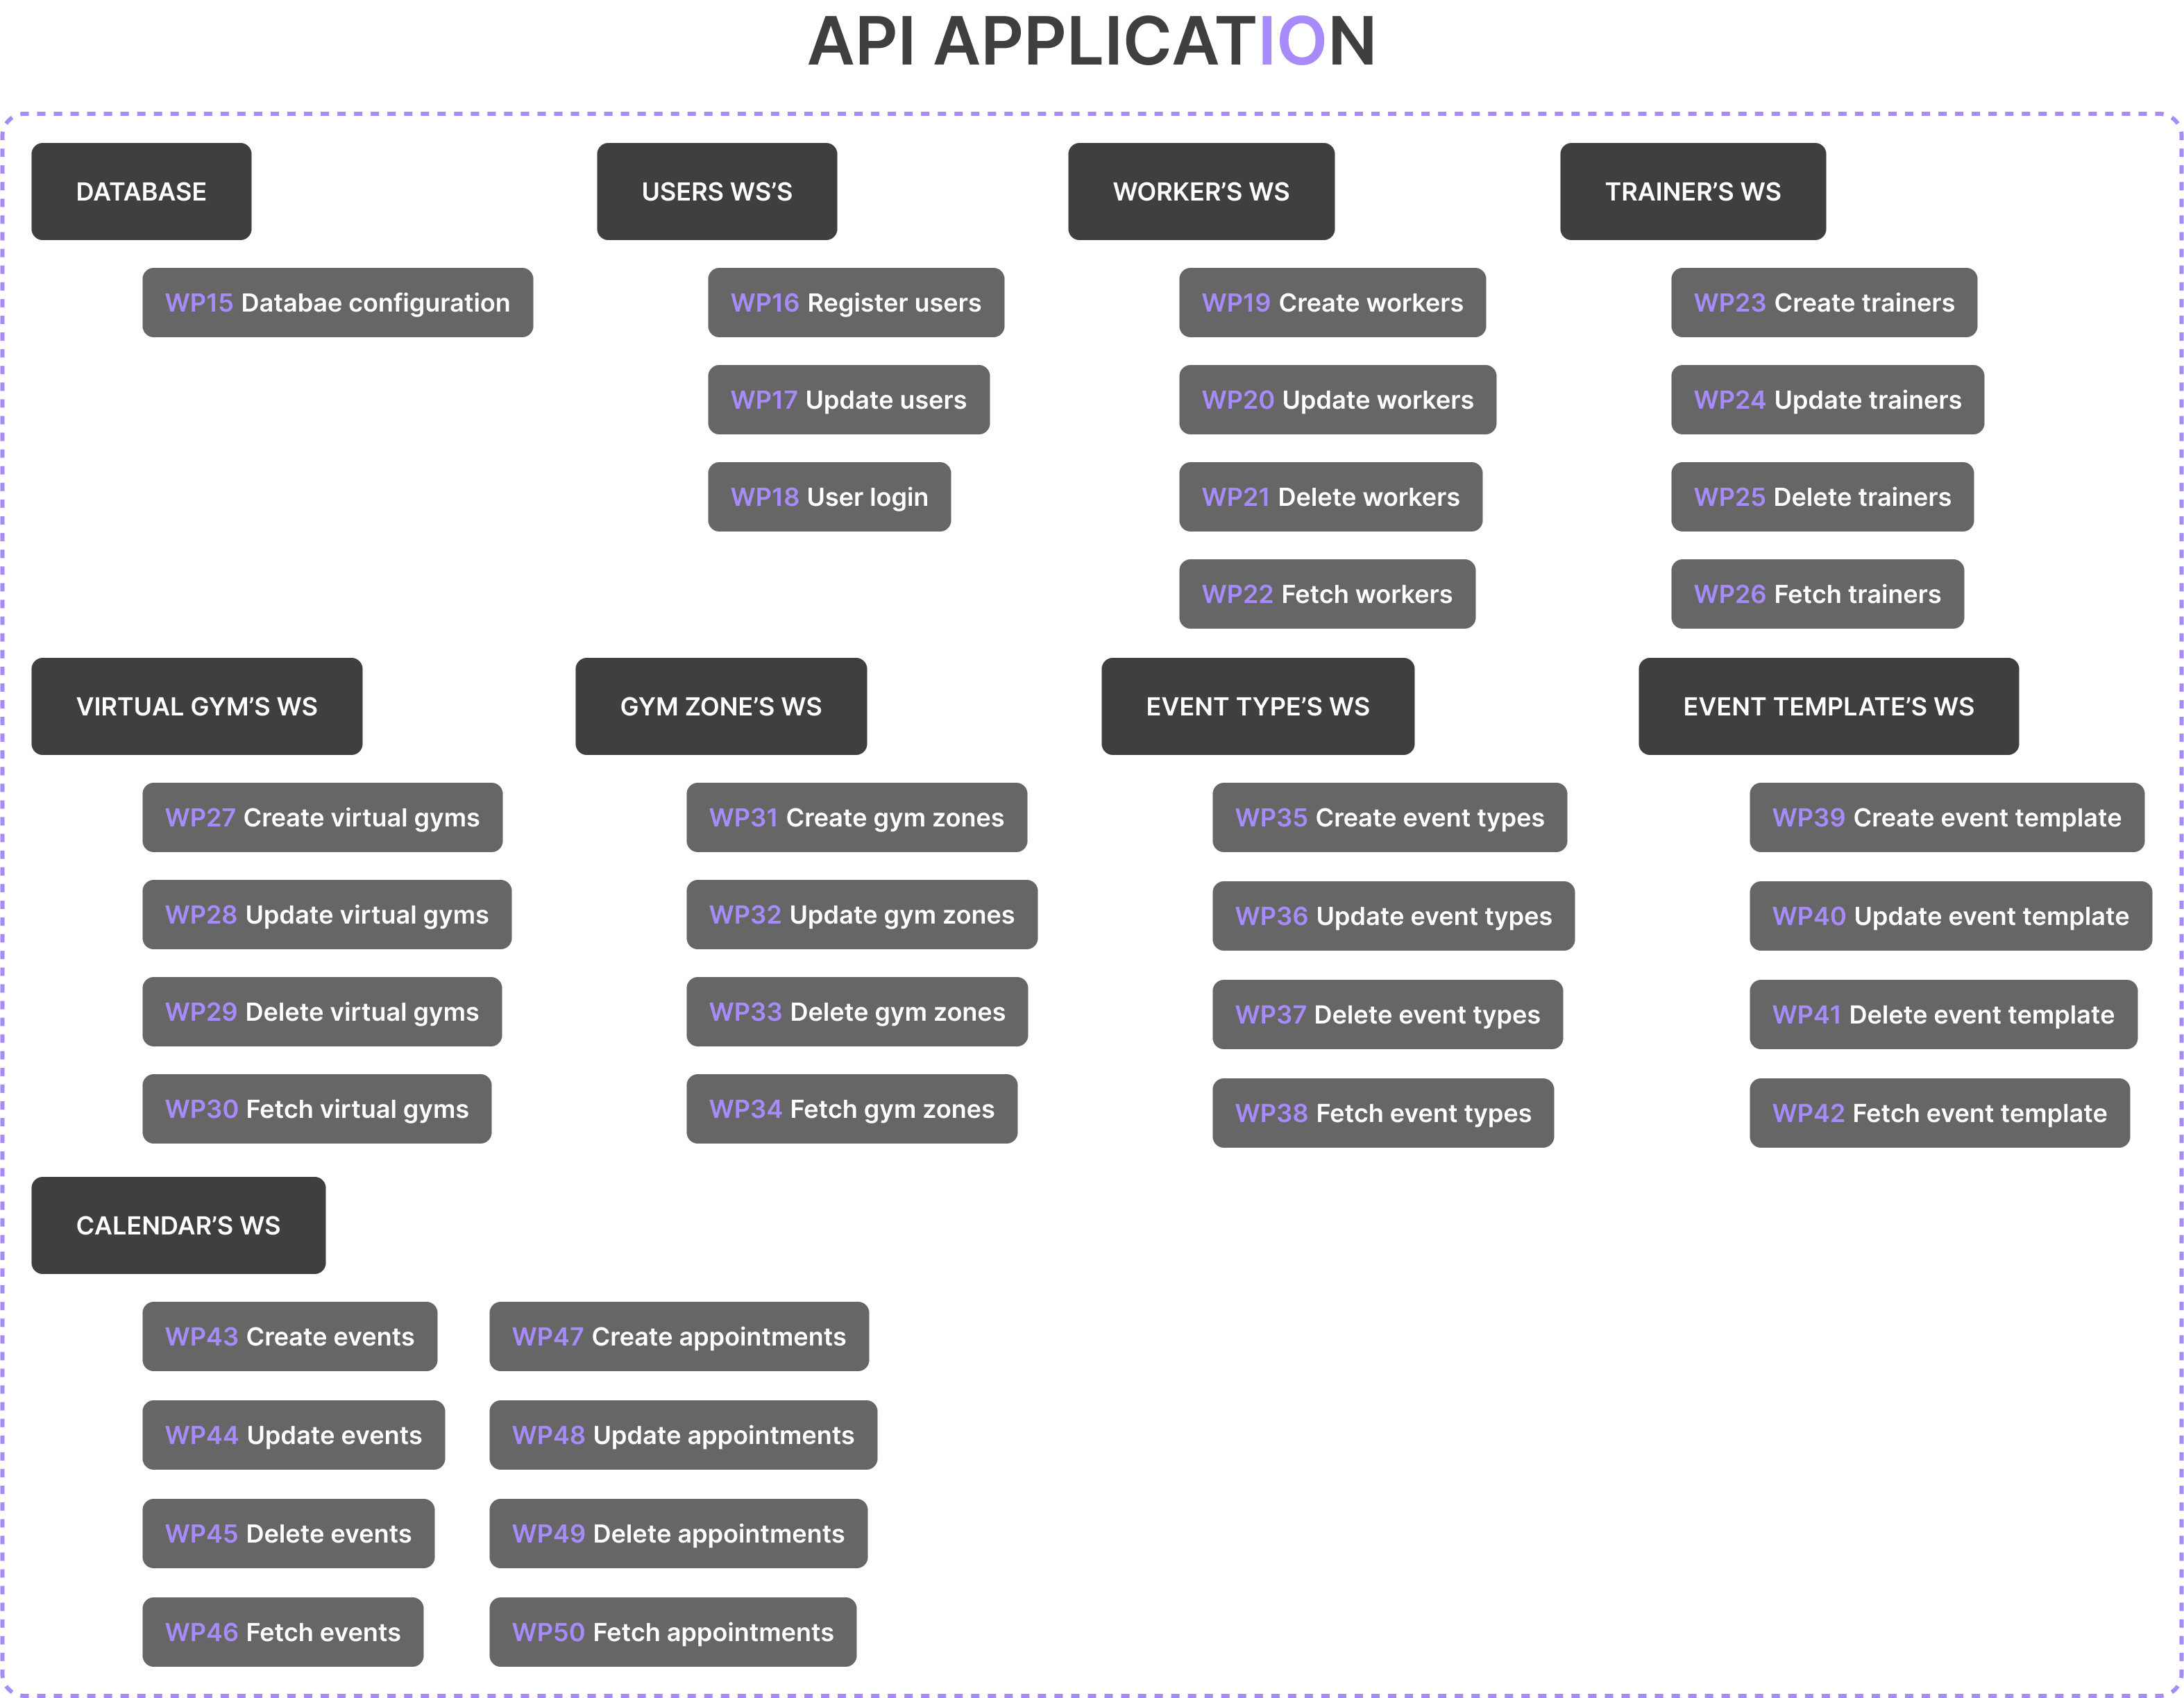
\includegraphics[width=\textwidth]{assets/working-packages/Api.png}
	\caption{Api application working packages diagram}
\end{figure}
The \emph{api} group is composed of the following working packages:
\\[8pt]
\begin{tabularx}{\textwidth}{| l | X |}
	\hline
	\rowcolor{rowColor}
	{\semibf Package name}   & {\semibf WP15}: Database configuration.                       \\
	\hline
	{\semibf Description}    & Configure the application so that is connected the database.  \\
	\hline
	\rowcolor{rowColor}
	{\semibf Estimated time} & 1h                                                            \\
	\hline
	{\semibf Tasks}          & {\semibf T1}: Configure the API with the dockerized database. \\
	\hline
	\rowcolor{rowColor}
	{\semibf Results}        & Connection of the api with the database.                      \\
	\hline
\end{tabularx}
\captionof{table}{Package fifteen's table - Database configuration}
\vspace*{16pt}
\begin{tabularx}{\textwidth}{| l | X |}
	\hline
	\rowcolor{rowColor}
	{\semibf Package name}   & {\semibf WP16}: Register users              \\
	\hline
	{\semibf Description}    & Allow the users to register.                \\
	\hline
	\rowcolor{rowColor}
	{\semibf Estimated time} & 8h                                          \\
	\hline
	{\semibf Tasks}          & {\semibf T1}: Create the services required.
	\newline {\semibf T2}: Create the controllers required.
	\newline {\semibf T3}: Create the owner register endpoint.
	\newline {\semibf T4}: Create the client register endpoint.            \\
	\hline
	\rowcolor{rowColor}
	{\semibf Results}        & Creation of a user.                         \\
	\hline
\end{tabularx}
\captionof{table}{Package sixteen's table - Register users}
\vspace*{16pt}
\begin{tabularx}{\textwidth}{| l | X |}
	\hline
	\rowcolor{rowColor}
	{\semibf Package name}   & {\semibf WP17}: Update users                 \\
	\hline
	{\semibf Description}    & Allow the users to update their information. \\
	\hline
	\rowcolor{rowColor}
	{\semibf Estimated time} & 4h                                           \\
	\hline
	{\semibf Tasks}          & {\semibf T1}: Create the services required.
	\newline {\semibf T2}: Create the controllers required.
	\newline {\semibf T3}: Create the user update endpoint.                 \\
	\hline
	\rowcolor{rowColor}
	{\semibf Results}        & Updation of user's information               \\
	\hline
\end{tabularx}
\captionof{table}{Package seventeen's table - Update users}
\vspace*{16pt}
\begin{tabularx}{\textwidth}{| l | X |}
	\hline
	\rowcolor{rowColor}
	{\semibf Package name}   & {\semibf WP18}: User login                         \\
	\hline
	{\semibf Description}    & Allow the users to log in to the application.      \\
	\hline
	\rowcolor{rowColor}
	{\semibf Estimated time} & 8h                                                 \\
	\hline
	{\semibf Tasks}          & {\semibf T1}: Create the services required.
	\newline {\semibf T2}: Create the controllers required.
	\newline {\semibf T3}: Create the session cookie validation endpoint.
	\newline {\semibf T4}: Create the login endpoint.                             \\
	\hline
	\rowcolor{rowColor}
	{\semibf Results}        & Endpoints to login and validate old user sessions. \\
	\hline
\end{tabularx}
\captionof{table}{Package eighteen's table - User login}
\vspace*{16pt}
\begin{tabularx}{\textwidth}{| l | X |}
	\hline
	\rowcolor{rowColor}
	{\semibf Package name}   & {\semibf WP19}: Create workers              \\
	\hline
	{\semibf Description}    & Allow the creation of workers.              \\
	\hline
	\rowcolor{rowColor}
	{\semibf Estimated time} & 6h                                          \\
	\hline
	{\semibf Tasks}          & {\semibf T1}: Create the services required.
	\newline {\semibf T2}: Create the controllers required.
	\newline {\semibf T3}: Create the workers create endpoint.             \\
	\hline
	\rowcolor{rowColor}
	{\semibf Results}        & Creation of workers.                        \\
	\hline
\end{tabularx}
\captionof{table}{Package nineteen's table - Create workers}
\vspace*{16pt}
\begin{tabularx}{\textwidth}{| l | X |}
	\hline
	\rowcolor{rowColor}
	{\semibf Package name}   & {\semibf WP20}: Update workers              \\
	\hline
	{\semibf Description}    & Allow the update of workers.                \\
	\hline
	\rowcolor{rowColor}
	{\semibf Estimated time} & 4h                                          \\
	\hline
	{\semibf Tasks}          & {\semibf T1}: Create the services required.
	\newline {\semibf T2}: Create the controllers required.
	\newline {\semibf T3}: Create the update workers endpoint.             \\
	\hline
	\rowcolor{rowColor}
	{\semibf Results}        & Updation of workers.                        \\
	\hline
\end{tabularx}
\captionof{table}{Package twenty's table - Update workers}
\vspace*{16pt}
\begin{tabularx}{\textwidth}{| l | X |}
	\hline
	\rowcolor{rowColor}
	{\semibf Package name}   & {\semibf WP21}: Delete workers              \\
	\hline
	{\semibf Description}    & Allow the deletion of workers.              \\
	\hline
	\rowcolor{rowColor}
	{\semibf Estimated time} & 4h                                          \\
	\hline
	{\semibf Tasks}          & {\semibf T1}: Create the services required.
	\newline {\semibf T2}: Create the controllers required.
	\newline {\semibf T3}: Create the delete workers endpoint.             \\
	\hline
	\rowcolor{rowColor}
	{\semibf Results}        & Deletion of workers.                        \\
	\hline
\end{tabularx}
\captionof{table}{Package twenty-one's table - Delete workers}
\vspace*{16pt}
\begin{tabularx}{\textwidth}{| l | X |}
	\hline
	\rowcolor{rowColor}
	{\semibf Package name}   & {\semibf WP22}: Fetch workers               \\
	\hline
	{\semibf Description}    & Allow the fetch of workers.                 \\
	\hline
	\rowcolor{rowColor}
	{\semibf Estimated time} & 4h                                          \\
	\hline
	{\semibf Tasks}          & {\semibf T1}: Create the services required.
	\newline {\semibf T2}: Create the controllers required.
	\newline {\semibf T3}: Create the fetch workers endpoint.              \\
	\hline
	\rowcolor{rowColor}
	{\semibf Results}        & Fetching of workers.                        \\
	\hline
\end{tabularx}
\captionof{table}{Package twenty-two's table - Fetch workers}
\vspace*{16pt}
\begin{tabularx}{\textwidth}{| l | X |}
	\hline
	\rowcolor{rowColor}
	{\semibf Package name}   & {\semibf WP23}: Create trainers             \\
	\hline
	{\semibf Description}    & Allow the creation of trainers.             \\
	\hline
	\rowcolor{rowColor}
	{\semibf Estimated time} & 8h                                          \\
	\hline
	{\semibf Tasks}          & {\semibf T1}: Create the services required.
	\newline {\semibf T2}: Create the controllers required.
	\newline {\semibf T3}: Create the create trainers endpoint.            \\
	\hline
	\rowcolor{rowColor}
	{\semibf Results}        & Creation of trainers.                       \\
	\hline
\end{tabularx}
\captionof{table}{Package twenty-three's table - Create trainers}
\vspace*{16pt}
\begin{tabularx}{\textwidth}{| l | X |}
	\hline
	\rowcolor{rowColor}
	{\semibf Package name}   & {\semibf WP24}: Update trainers             \\
	\hline
	{\semibf Description}    & Allow the update of trainers.               \\
	\hline
	\rowcolor{rowColor}
	{\semibf Estimated time} & 4h                                          \\
	\hline
	{\semibf Tasks}          & {\semibf T1}: Create the services required.
	\newline {\semibf T2}: Create the controllers required.
	\newline {\semibf T3}: Create the update trainers endpoint.            \\
	\hline
	\rowcolor{rowColor}
	{\semibf Results}        & Updation of trainers.                       \\
	\hline
\end{tabularx}
\captionof{table}{Package twenty-four's table - Update trainers}
\vspace*{16pt}
\begin{tabularx}{\textwidth}{| l | X |}
	\hline
	\rowcolor{rowColor}
	{\semibf Package name}   & {\semibf WP25}: Delete trainers             \\
	\hline
	{\semibf Description}    & Allow the deletion of trainers.             \\
	\hline
	\rowcolor{rowColor}
	{\semibf Estimated time} & 4h                                          \\
	\hline
	{\semibf Tasks}          & {\semibf T1}: Create the services required.
	\newline {\semibf T2}: Create the controllers required.
	\newline {\semibf T3}: Create the delete trainers endpoint.            \\
	\hline
	\rowcolor{rowColor}
	{\semibf Results}        & Deletion of trainers.                       \\
	\hline
\end{tabularx}
\captionof{table}{Package twenty-five's table - Delete trainers}
\vspace*{16pt}
\begin{tabularx}{\textwidth}{| l | X |}
	\hline
	\rowcolor{rowColor}
	{\semibf Package name}   & {\semibf WP26}: Fetch trainers              \\
	\hline
	{\semibf Description}    & Allow the fetch of trainers.                \\
	\hline
	\rowcolor{rowColor}
	{\semibf Estimated time} & 4h                                          \\
	\hline
	{\semibf Tasks}          & {\semibf T1}: Create the services required.
	\newline {\semibf T2}: Create the controllers required.
	\newline {\semibf T3}: Create the fetch trainers endpoint.             \\
	\hline
	\rowcolor{rowColor}
	{\semibf Results}        & Fetching of trainers.                       \\
	\hline
\end{tabularx}
\captionof{table}{Package twenty-six's table - Fetch trainers}
\vspace*{16pt}
\begin{tabularx}{\textwidth}{| l | X |}
	\hline
	\rowcolor{rowColor}
	{\semibf Package name}   & {\semibf WP27}: Create virtual gyms         \\
	\hline
	{\semibf Description}    & Allow the creation of virtual gyms.         \\
	\hline
	\rowcolor{rowColor}
	{\semibf Estimated time} & 8h                                          \\
	\hline
	{\semibf Tasks}          & {\semibf T1}: Create the services required.
	\newline {\semibf T2}: Create the controllers required.
	\newline {\semibf T3}: Create the virtual gym creation endpoint.       \\
	\hline
	\rowcolor{rowColor}
	{\semibf Results}        & Creation of virtual gyms.                   \\
	\hline
\end{tabularx}
\captionof{table}{Package twenty-seven's table - Create virtual gyms}
\vspace*{16pt}
\begin{tabularx}{\textwidth}{| l | X |}
	\hline
	\rowcolor{rowColor}
	{\semibf Package name}   & {\semibf WP28}: Update virtual gyms         \\
	\hline
	{\semibf Description}    & Allow the update of virtual gyms.           \\
	\hline
	\rowcolor{rowColor}
	{\semibf Estimated time} & 4h                                          \\
	\hline
	{\semibf Tasks}          & {\semibf T1}: Create the services required.
	\newline {\semibf T2}: Create the controllers required.
	\newline {\semibf T3}: Create the virtual gym update endpoint.         \\
	\hline
	\rowcolor{rowColor}
	{\semibf Results}        & Updation of virtual gyms.                   \\
	\hline
\end{tabularx}
\captionof{table}{Package twenty-eight's table - Update virtual gyms}
\vspace*{16pt}
\begin{tabularx}{\textwidth}{| l | X |}
	\hline
	\rowcolor{rowColor}
	{\semibf Package name}   & {\semibf WP29}: Delete virtual gyms         \\
	\hline
	{\semibf Description}    & Allow the deletion of virtual gyms.         \\
	\hline
	\rowcolor{rowColor}
	{\semibf Estimated time} & 4h                                          \\
	\hline
	{\semibf Tasks}          & {\semibf T1}: Create the services required.
	\newline {\semibf T2}: Create the controllers required.
	\newline {\semibf T3}: Create the virtual gym deletion endpoint.       \\
	\hline
	\rowcolor{rowColor}
	{\semibf Results}        & Deletion of virtual gyms.                   \\
	\hline
\end{tabularx}
\captionof{table}{Package twenty-nine's table - Delete virtual gyms}
\vspace*{16pt}
\begin{tabularx}{\textwidth}{| l | X |}
	\hline
	\rowcolor{rowColor}
	{\semibf Package name}   & {\semibf WP30}: Fetch virtual gyms          \\
	\hline
	{\semibf Description}    & Allow the fetch of virtual gyms.            \\
	\hline
	\rowcolor{rowColor}
	{\semibf Estimated time} & 4h                                          \\
	\hline
	{\semibf Tasks}          & {\semibf T1}: Create the services required.
	\newline {\semibf T2}: Create the controllers required.
	\newline {\semibf T3}: Create the virtual gym fetch endpoint.          \\
	\hline
	\rowcolor{rowColor}
	{\semibf Results}        & Fetching of virtual gyms.                   \\
	\hline
\end{tabularx}
\captionof{table}{Package thirty's table - Delete virtual gyms}
\vspace*{16pt}
\begin{tabularx}{\textwidth}{| l | X |}
	\hline
	\rowcolor{rowColor}
	{\semibf Package name}   & {\semibf WP31}: Create gym zones            \\
	\hline
	{\semibf Description}    & Allow the creation of gym zones.            \\
	\hline
	\rowcolor{rowColor}
	{\semibf Estimated time} & 8h                                          \\
	\hline
	{\semibf Tasks}          & {\semibf T1}: Create the services required.
	\newline {\semibf T2}: Create the controllers required.
	\newline {\semibf T3}: Create the gym zone create endpoint.            \\
	\hline
	\rowcolor{rowColor}
	{\semibf Results}        & Creation of gym zones.                      \\
	\hline
\end{tabularx}
\captionof{table}{Package thirty-one's table - Create gym zones}
\vspace*{16pt}
\begin{tabularx}{\textwidth}{| l | X |}
	\hline
	\rowcolor{rowColor}
	{\semibf Package name}   & {\semibf WP32}: Update gym zones            \\
	\hline
	{\semibf Description}    & Allow the update of gym zones.              \\
	\hline
	\rowcolor{rowColor}
	{\semibf Estimated time} & 4h                                          \\
	\hline
	{\semibf Tasks}          & {\semibf T1}: Create the services required.
	\newline {\semibf T2}: Create the controllers required.
	\newline {\semibf T3}: Create the gym zone update endpoint.            \\
	\hline
	\rowcolor{rowColor}
	{\semibf Results}        & Updation of gym zones.                      \\
	\hline
\end{tabularx}
\captionof{table}{Package thirty-two's table - Update gym zones}
\vspace*{16pt}
\begin{tabularx}{\textwidth}{| l | X |}
	\hline
	\rowcolor{rowColor}
	{\semibf Package name}   & {\semibf WP33}: Delete gym zones            \\
	\hline
	{\semibf Description}    & Allow the deletion of gym zones.            \\
	\hline
	\rowcolor{rowColor}
	{\semibf Estimated time} & 4h                                          \\
	\hline
	{\semibf Tasks}          & {\semibf T1}: Create the services required.
	\newline {\semibf T2}: Create the controllers required.
	\newline {\semibf T3}: Create the gym zone delete endpoint.            \\
	\hline
	\rowcolor{rowColor}
	{\semibf Results}        & Deletion of gym zones.                      \\
	\hline
\end{tabularx}
\captionof{table}{Package thirty-three's table - Delete gym zones}
\vspace*{16pt}
\begin{tabularx}{\textwidth}{| l | X |}
	\hline
	\rowcolor{rowColor}
	{\semibf Package name}   & {\semibf WP34}: Fetch gym zones             \\
	\hline
	{\semibf Description}    & Allow the fetching of gym zones.            \\
	\hline
	\rowcolor{rowColor}
	{\semibf Estimated time} & 4h                                          \\
	\hline
	{\semibf Tasks}          & {\semibf T1}: Create the services required.
	\newline {\semibf T2}: Create the controllers required.
	\newline {\semibf T3}: Create the gym zone fetch endpoint.             \\
	\hline
	\rowcolor{rowColor}
	{\semibf Results}        & Fetching of gym zones.                      \\
	\hline
\end{tabularx}
\captionof{table}{Package thirty-four's table - Fetch gym zones}
\vspace*{16pt}
\begin{tabularx}{\textwidth}{| l | X |}
	\hline
	\rowcolor{rowColor}
	{\semibf Package name}   & {\semibf WP35}: Create event types          \\
	\hline
	{\semibf Description}    & Allow the creation of event types.          \\
	\hline
	\rowcolor{rowColor}
	{\semibf Estimated time} & 8h                                          \\
	\hline
	{\semibf Tasks}          & {\semibf T1}: Create the services required.
	\newline {\semibf T2}: Create the controllers required.
	\newline {\semibf T3}: Create the event types create endpoint.         \\
	\hline
	\rowcolor{rowColor}
	{\semibf Results}        & Creation of event types.                    \\
	\hline
\end{tabularx}
\captionof{table}{Package thirty-five's table - Create event types}
\vspace*{16pt}
\begin{tabularx}{\textwidth}{| l | X |}
	\hline
	\rowcolor{rowColor}
	{\semibf Package name}   & {\semibf WP36}: Update event types          \\
	\hline
	{\semibf Description}    & Allow the update of event types.            \\
	\hline
	\rowcolor{rowColor}
	{\semibf Estimated time} & 4h                                          \\
	\hline
	{\semibf Tasks}          & {\semibf T1}: Create the services required.
	\newline {\semibf T2}: Create the controllers required.
	\newline {\semibf T3}: Create the event types update endpoint.         \\
	\hline
	\rowcolor{rowColor}
	{\semibf Results}        & Updation of event types.                    \\
	\hline
\end{tabularx}
\captionof{table}{Package thirty-six's table - Update event types}
\vspace*{16pt}
\begin{tabularx}{\textwidth}{| l | X |}
	\hline
	\rowcolor{rowColor}
	{\semibf Package name}   & {\semibf WP37}: Delete event types          \\
	\hline
	{\semibf Description}    & Allow the deletion of event types.          \\
	\hline
	\rowcolor{rowColor}
	{\semibf Estimated time} & 4h                                          \\
	\hline
	{\semibf Tasks}          & {\semibf T1}: Create the services required.
	\newline {\semibf T2}: Create the controllers required.
	\newline {\semibf T3}: Create the event types delete endpoint.         \\
	\hline
	\rowcolor{rowColor}
	{\semibf Results}        & Updation of event types.                    \\
	\hline
\end{tabularx}
\captionof{table}{Package thirty-seven's table - Delete event types}
\vspace*{16pt}
\begin{tabularx}{\textwidth}{| l | X |}
	\hline
	\rowcolor{rowColor}
	{\semibf Package name}   & {\semibf WP38}: Fetch event types           \\
	\hline
	{\semibf Description}    & Allow the fetch of event types.             \\
	\hline
	\rowcolor{rowColor}
	{\semibf Estimated time} & 4h                                          \\
	\hline
	{\semibf Tasks}          & {\semibf T1}: Create the services required.
	\newline {\semibf T2}: Create the controllers required.
	\newline {\semibf T3}: Create the event types fetch endpoint.          \\
	\hline
	\rowcolor{rowColor}
	{\semibf Results}        & Fetching of event types.                    \\
	\hline
\end{tabularx}
\captionof{table}{Package thirty-eight's table - Fetch event types}
\vspace*{16pt}
\begin{tabularx}{\textwidth}{| l | X |}
	\hline
	\rowcolor{rowColor}
	{\semibf Package name}   & {\semibf WP39}: Create event templates      \\
	\hline
	{\semibf Description}    & Allow the creation of event templates.      \\
	\hline
	\rowcolor{rowColor}
	{\semibf Estimated time} & 4h                                          \\
	\hline
	{\semibf Tasks}          & {\semibf T1}: Create the services required.
	\newline {\semibf T2}: Create the controllers required.
	\newline {\semibf T3}: Create the event templates create endpoint.     \\
	\hline
	\rowcolor{rowColor}
	{\semibf Results}        & Creation of event templates.                \\
	\hline
\end{tabularx}
\captionof{table}{Package thirty-nine's table - Create event templates}
\vspace*{16pt}
\begin{tabularx}{\textwidth}{| l | X |}
	\hline
	\rowcolor{rowColor}
	{\semibf Package name}   & {\semibf WP40}: Update event templates      \\
	\hline
	{\semibf Description}    & Allow the update of event templates.        \\
	\hline
	\rowcolor{rowColor}
	{\semibf Estimated time} & 4h                                          \\
	\hline
	{\semibf Tasks}          & {\semibf T1}: Create the services required.
	\newline {\semibf T2}: Create the controllers required.
	\newline {\semibf T3}: Create the event templates update endpoint.     \\
	\hline
	\rowcolor{rowColor}
	{\semibf Results}        & Updation of event templates.                \\
	\hline
\end{tabularx}
\captionof{table}{Package forty's table - Update event templates}
\vspace*{16pt}
\begin{tabularx}{\textwidth}{| l | X |}
	\hline
	\rowcolor{rowColor}
	{\semibf Package name}   & {\semibf WP41}: Delete event templates      \\
	\hline
	{\semibf Description}    & Allow the deletion of event templates.      \\
	\hline
	\rowcolor{rowColor}
	{\semibf Estimated time} & 4h                                          \\
	\hline
	{\semibf Tasks}          & {\semibf T1}: Create the services required.
	\newline {\semibf T2}: Create the controllers required.
	\newline {\semibf T3}: Create the event templates delete endpoint.     \\
	\hline
	\rowcolor{rowColor}
	{\semibf Results}        & Deletion of event templates.                \\
	\hline
\end{tabularx}
\captionof{table}{Package forty-one's table - Delete event templates}
\vspace*{16pt}
\begin{tabularx}{\textwidth}{| l | X |}
	\hline
	\rowcolor{rowColor}
	{\semibf Package name}   & {\semibf WP42}: Fetch event templates       \\
	\hline
	{\semibf Description}    & Allow the fetch of event templates.         \\
	\hline
	\rowcolor{rowColor}
	{\semibf Estimated time} & 4h                                          \\
	\hline
	{\semibf Tasks}          & {\semibf T1}: Create the services required.
	\newline {\semibf T2}: Create the controllers required.
	\newline {\semibf T3}: Create the event templates fetch endpoint.      \\
	\hline
	\rowcolor{rowColor}
	{\semibf Results}        & Fetching of event templates.                \\
	\hline
\end{tabularx}
\captionof{table}{Package forty-two's table - Fetch event templates}
\vspace*{16pt}
\begin{tabularx}{\textwidth}{| l | X |}
	\hline
	\rowcolor{rowColor}
	{\semibf Package name}   & {\semibf WP43}: Create events               \\
	\hline
	{\semibf Description}    & Allow the creation of events.               \\
	\hline
	\rowcolor{rowColor}
	{\semibf Estimated time} & 8h                                          \\
	\hline
	{\semibf Tasks}          & {\semibf T1}: Create the services required.
	\newline {\semibf T2}: Create the controllers required.
	\newline {\semibf T3}: Create the events fetch endpoint.               \\
	\hline
	\rowcolor{rowColor}
	{\semibf Results}        & Creation of events.                         \\
	\hline
\end{tabularx}
\captionof{table}{Package forty-three's table - Create events}
\vspace*{16pt}
\begin{tabularx}{\textwidth}{| l | X |}
	\hline
	\rowcolor{rowColor}
	{\semibf Package name}   & {\semibf WP44}: Update events               \\
	\hline
	{\semibf Description}    & Allow the update of events.                 \\
	\hline
	\rowcolor{rowColor}
	{\semibf Estimated time} & 4h                                          \\
	\hline
	{\semibf Tasks}          & {\semibf T1}: Create the services required.
	\newline {\semibf T2}: Create the controllers required.
	\newline {\semibf T3}: Create the events update endpoint.              \\
	\hline
	\rowcolor{rowColor}
	{\semibf Results}        & Updation of events.                         \\
	\hline
\end{tabularx}
\captionof{table}{Package forty-four's table - Update events}
\vspace*{16pt}
\begin{tabularx}{\textwidth}{| l | X |}
	\hline
	\rowcolor{rowColor}
	{\semibf Package name}   & {\semibf WP45}: Delete events               \\
	\hline
	{\semibf Description}    & Allow the deletion of events.               \\
	\hline
	\rowcolor{rowColor}
	{\semibf Estimated time} & 4h                                          \\
	\hline
	{\semibf Tasks}          & {\semibf T1}: Create the services required.
	\newline {\semibf T2}: Create the controllers required.
	\newline {\semibf T3}: Create the events delete endpoint.              \\
	\hline
	\rowcolor{rowColor}
	{\semibf Results}        & Deletion of events.                         \\
	\hline
\end{tabularx}
\captionof{table}{Package forty-five's table - Delete events}
\vspace*{16pt}
\begin{tabularx}{\textwidth}{| l | X |}
	\hline
	\rowcolor{rowColor}
	{\semibf Package name}   & {\semibf WP46}: Fetch events                \\
	\hline
	{\semibf Description}    & Allow the fetching of events.               \\
	\hline
	\rowcolor{rowColor}
	{\semibf Estimated time} & 4h                                          \\
	\hline
	{\semibf Tasks}          & {\semibf T1}: Create the services required.
	\newline {\semibf T2}: Create the controllers required.
	\newline {\semibf T3}: Create the events fetch endpoint.               \\
	\hline
	\rowcolor{rowColor}
	{\semibf Results}        & Fetching of events.                         \\
	\hline
\end{tabularx}
\captionof{table}{Package forty-six's table - Fetch events}
\vspace*{16pt}
\begin{tabularx}{\textwidth}{| l | X |}
	\hline
	\rowcolor{rowColor}
	{\semibf Package name}   & {\semibf WP47}: Create appointments                                             \\
	\hline
	{\semibf Description}    & Allow the fetching of appointments. It is important to create an algorithm that
	ensures that a gym zone does not have more appointments than its capacity.                                 \\
	\hline
	\rowcolor{rowColor}
	{\semibf Estimated time} & 16h                                                                              \\
	\hline
	{\semibf Tasks}          & {\semibf T1}: Create the services required.
	\newline {\semibf T2}: Create the controllers required.
	\newline {\semibf T3}: Create the available hours endpoint.
	\newline {\semibf T4}: Create the appointments create endpoint.                                            \\
	\hline
	\rowcolor{rowColor}
	{\semibf Results}        & Creation of appointments.                                                       \\
	\hline
\end{tabularx}
\captionof{table}{Package forty-seven's table - Create appointments}
\vspace*{16pt}
\begin{tabularx}{\textwidth}{| l | X |}
	\hline
	\rowcolor{rowColor}
	{\semibf Package name}   & {\semibf WP48}: Update appointments                              \\
	\hline
	{\semibf Description}    & Allow the update of appointments. It should only allow to cancel
	the appointment.                                                                            \\
	\hline
	\rowcolor{rowColor}
	{\semibf Estimated time} & 4h                                                               \\
	\hline
	{\semibf Tasks}          & {\semibf T1}: Create the services required.
	\newline {\semibf T2}: Create the controllers required.
	\newline {\semibf T4}: Create the appointments update endpoint.                             \\
	\hline
	\rowcolor{rowColor}
	{\semibf Results}        & Updation of appointments.                                        \\
	\hline
\end{tabularx}
\captionof{table}{Package forty-eight's table - Update appointments}
\vspace*{16pt}
\begin{tabularx}{\textwidth}{| l | X |}
	\hline
	\rowcolor{rowColor}
	{\semibf Package name}   & {\semibf WP49}: Delete appointments                                \\
	\hline
	{\semibf Description}    & Allow the deletion of appointments. It should only allow to cancel
	the appointment.                                                                              \\
	\hline
	\rowcolor{rowColor}
	{\semibf Estimated time} & 4h                                                                 \\
	\hline
	{\semibf Tasks}          & {\semibf T1}: Create the services required.
	\newline {\semibf T2}: Create the controllers required.
	\newline {\semibf T4}: Create the appointments delete endpoint.                               \\
	\hline
	\rowcolor{rowColor}
	{\semibf Results}        & Deletion of appointments.                                          \\
	\hline
\end{tabularx}
\captionof{table}{Package forty-nine's table - Delete appointments}
\vspace*{16pt}
\begin{tabularx}{\textwidth}{| l | X |}
	\hline
	\rowcolor{rowColor}
	{\semibf Package name}   & {\semibf WP50}: Fetch appointments          \\
	\hline
	{\semibf Description}    & Allow the fetch of appointments.            \\
	\hline
	\rowcolor{rowColor}
	{\semibf Estimated time} & 6h                                          \\
	\hline
	{\semibf Tasks}          & {\semibf T1}: Create the services required.
	\newline {\semibf T2}: Create the controllers required.
	\newline {\semibf T4}: Create the appointments fetch endpoint.         \\
	\hline
	\rowcolor{rowColor}
	{\semibf Results}        & Fetching of appointments.                   \\
	\hline
\end{tabularx}
\captionof{table}{Package fifty's table - Fetch appointments}
\subsubsection{Core application}
The \emph{core} group of working packages follows a similar approach as the one described in \nameref{working-packages-development}.
\begin{figure}[H]
	\centering
	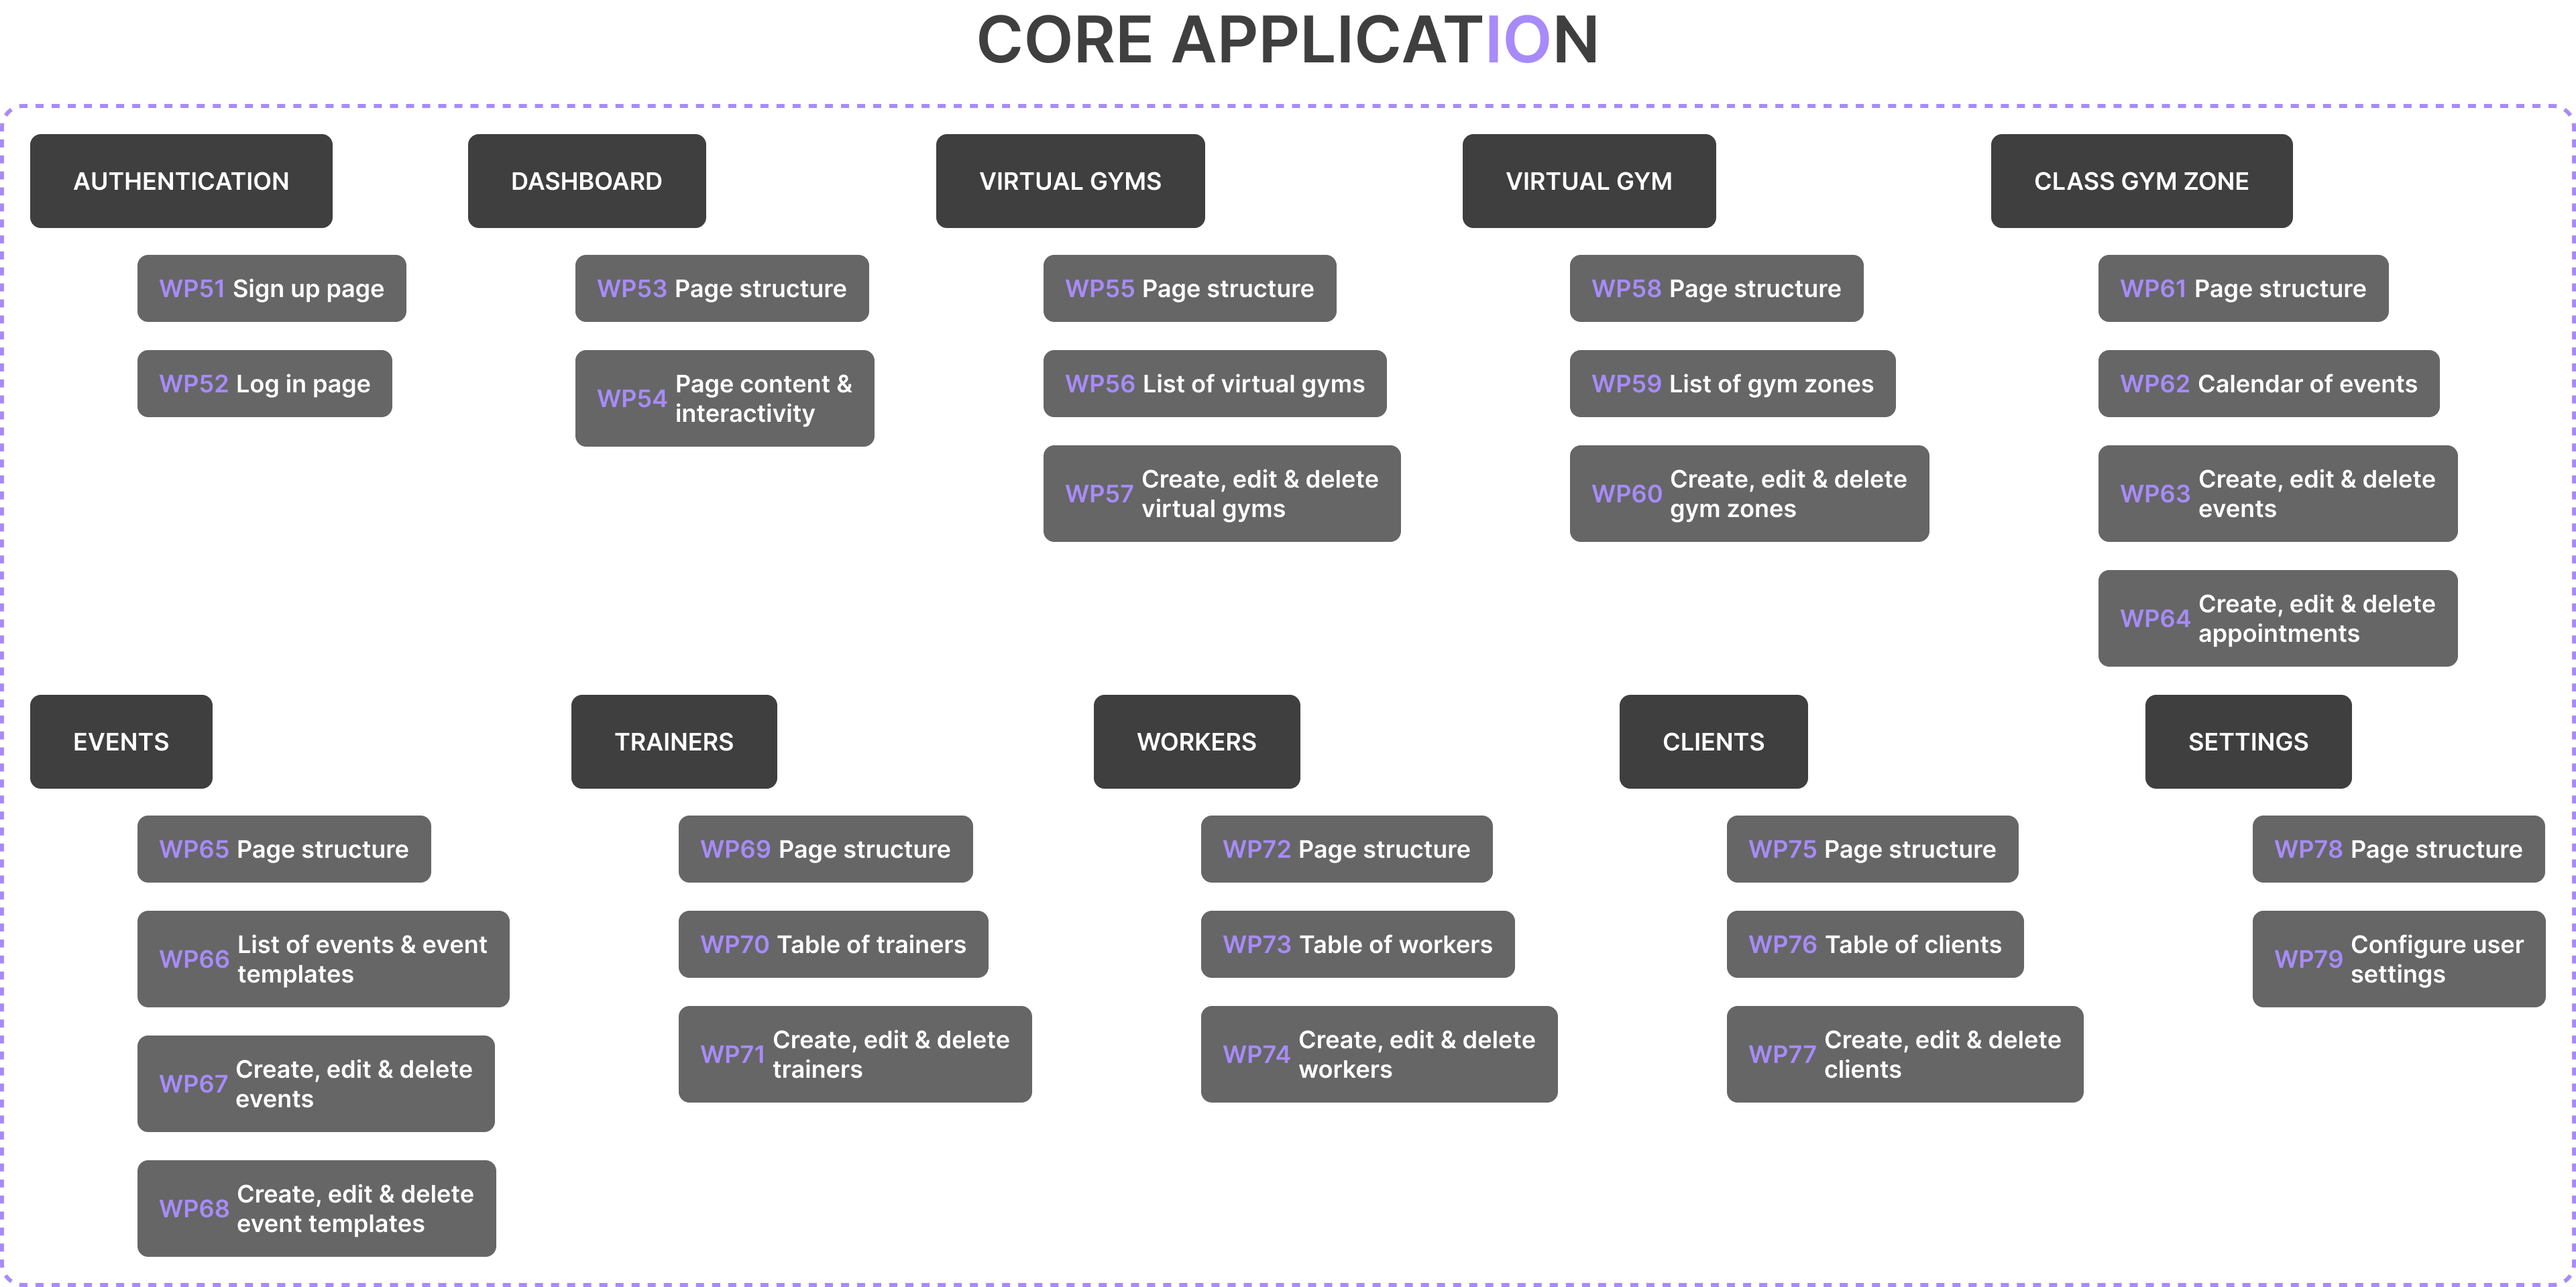
\includegraphics[width=\textwidth]{assets/working-packages/Core.png}
	\caption{Core application working packages diagram}
\end{figure}
The \emph{core} group is composed of the following working packages:
\\[8pt]
\begin{tabularx}{\textwidth}{| l | X |}
	\hline
	\rowcolor{rowColor}
	{\semibf Package name}   & {\semibf WP51}: Sign up page               \\
	\hline
	{\semibf Description}    & Develop the sign up page                   \\
	\hline
	\rowcolor{rowColor}
	{\semibf Estimated time} & 16h                                         \\
	\hline
	{\semibf Tasks}          & {\semibf T1}: Set up the page structure.
	\newline {\semibf T2}: Sign up as an owner.                           \\
	\hline
	\rowcolor{rowColor}
	{\semibf Results}        & Allow the users to register to the system. \\
	\hline
\end{tabularx}
\captionof{table}{Package fifty-one's table - Sign up page}
\vspace*{16pt}
\begin{tabularx}{\textwidth}{| l | X |}
	\hline
	\rowcolor{rowColor}
	{\semibf Package name}   & {\semibf WP52}: Log in page              \\
	\hline
	{\semibf Description}    & Develop the log in page.                 \\
	\hline
	\rowcolor{rowColor}
	{\semibf Estimated time} & 16h                                       \\
	\hline
	{\semibf Tasks}          & {\semibf T1}: Set up the page structure.
	\newline {\semibf T2}: Log in as an owner.
	\newline {\semibf T3}: Log in as a worker.                          \\
	\hline
	\rowcolor{rowColor}
	{\semibf Results}        & Allow the user to log in to the system.  \\
	\hline
\end{tabularx}
\captionof{table}{Package fifty-two's table - Log in page}
\vspace*{16pt}
\begin{tabularx}{\textwidth}{| l | X |}
	\hline
	\rowcolor{rowColor}
	{\semibf Package name}   & {\semibf WP53}: Page structure (Dashboard)            \\
	\hline
	{\semibf Description}    & Apply the design of the dashboard page.               \\
	\hline
	\rowcolor{rowColor}
	{\semibf Estimated time} & 4h                                                    \\
	\hline
	{\semibf Tasks}          & {\semibf T1}: Apply the design of the dashboard page. \\
	\hline
	\rowcolor{rowColor}
	{\semibf Results}        & The scaffolding of the dashboard page.                \\
	\hline
\end{tabularx}
\captionof{table}{Package fifty-three's table - Page structure (Dashboard)}
\vspace*{16pt}
\begin{tabularx}{\textwidth}{| l | X |}
	\hline
	\rowcolor{rowColor}
	{\semibf Package name}   & {\semibf WP54}: Page content and interactivity (Dashboard) \\
	\hline
	{\semibf Description}    & Add the interactivity to the dashboard page.               \\
	\hline
	\rowcolor{rowColor}
	{\semibf Estimated time} & 12h                                                      \\
	\hline
	{\semibf Tasks}          & {\semibf T1}: Add virtual gyms' interactivity.
	\newline {\semibf T2}: Add gym zones' interactivity.
	\newline {\semibf T3}: Add trainers' interactivity.
	\newline {\semibf T4}: Add event templates' interactivity.
	\newline {\semibf T5}: Add events' interactivity.                                     \\
	\hline
	\rowcolor{rowColor}
	{\semibf Results}        & User experience of the dasboard page.                      \\
	\hline
\end{tabularx}
\captionof{table}{Package fifty-four's table - Page content and interactivity}
\vspace*{16pt}
\begin{tabularx}{\textwidth}{| l | X |}
	\hline
	\rowcolor{rowColor}
	{\semibf Package name}   & {\semibf WP55}: Page structure (Virtual gyms)            \\
	\hline
	{\semibf Description}    & Apply the design of the virtual gyms page.               \\
	\hline
	\rowcolor{rowColor}
	{\semibf Estimated time} & 4h                                                       \\
	\hline
	{\semibf Tasks}          & {\semibf T1}: Apply the design of the virtual gyms page. \\
	\hline
	\rowcolor{rowColor}
	{\semibf Results}        & The scaffolding of the virtual gyms page.                \\
	\hline
\end{tabularx}
\captionof{table}{Package fifty-five's table - Page structure (Virtual gyms)}
\vspace*{16pt}
\begin{tabularx}{\textwidth}{| l | X |}
	\hline
	\rowcolor{rowColor}
	{\semibf Package name}   & {\semibf WP56}: List of virtual gyms (Virtual gyms) \\
	\hline
	{\semibf Description}    & Display the list of virtual gyms.                   \\
	\hline
	\rowcolor{rowColor}
	{\semibf Estimated time} & 4h                                                  \\
	\hline
	{\semibf Tasks}          & {\semibf T1}: List the virtual gyms of the gym.
	\newline {\semibf T2}: List the gym zones inside each virtual gym.             \\
	\hline
	\rowcolor{rowColor}
	{\semibf Results}        & The page of virtual gyms.                           \\
	\hline
\end{tabularx}
\captionof{table}{Package fifty-six's table - List of virtual gyms (Virtual gyms)}
\vspace*{16pt}
\begin{tabularx}{\textwidth}{| l | X |}
	\hline
	\rowcolor{rowColor}
	{\semibf Package name}   & {\semibf WP57}: Create, edit and delete virtual gyms (Virtual gyms) \\
	\hline
	{\semibf Description}    & Create the modal to create, edit and delete virtual gyms.           \\
	\hline
	\rowcolor{rowColor}
	{\semibf Estimated time} & 8h                                                                  \\
	\hline
	{\semibf Tasks}          & {\semibf T1}: Modal to create, edit and delete virtual gyms.        \\
	\hline
	\rowcolor{rowColor}
	{\semibf Results}        & The modal to interact with virtual gyms.                            \\
	\hline
\end{tabularx}
\captionof{table}{Package fifty-seven's table - List of virtual gyms (Virtual gyms)}
\vspace*{16pt}
\begin{tabularx}{\textwidth}{| l | X |}
	\hline
	\rowcolor{rowColor}
	{\semibf Package name}   & {\semibf WP58}: Page structure (Virtual gym)            \\
	\hline
	{\semibf Description}    & Apply the design of the virtual gym page.               \\
	\hline
	\rowcolor{rowColor}
	{\semibf Estimated time} & 4h                                                      \\
	\hline
	{\semibf Tasks}          & {\semibf T1}: Apply the design of the virtual gym page. \\
	\hline
	\rowcolor{rowColor}
	{\semibf Results}        & The scaffolding of the virtual gym page.                \\
	\hline
\end{tabularx}
\captionof{table}{Package fitfty-eight's table - Page structure (Virtual gym)}
\vspace*{16pt}
\begin{tabularx}{\textwidth}{| l | X |}
	\hline
	\rowcolor{rowColor}
	{\semibf Package name}   & {\semibf WP59}: List of gym zones (Virtual gym) \\
	\hline
	{\semibf Description}    & List the gym zones of a virtual gym.            \\
	\hline
	\rowcolor{rowColor}
	{\semibf Estimated time} & 8h                                              \\
	\hline
	{\semibf Tasks}          & {\semibf T1}: List all class gym zones.
	\newline {\semibf T2}: List all non-class gym zones.                       \\
	\hline
	\rowcolor{rowColor}
	{\semibf Results}        & The page of a virtual gym.                      \\
	\hline
\end{tabularx}
\captionof{table}{Package fifty-nine's table - List of gym zones (Virtual gym)}
\vspace*{16pt}
\begin{tabularx}{\textwidth}{| l | X |}
	\hline
	\rowcolor{rowColor}
	{\semibf Package name}   & {\semibf WP60}: Create, edit and delete gym zones (Virtual gym) \\
	\hline
	{\semibf Description}    & Create the modal to create, edit and delete gym zones.          \\
	\hline
	\rowcolor{rowColor}
	{\semibf Estimated time} & 8h                                                              \\
	\hline
	{\semibf Tasks}          & {\semibf T1}: Modal to create, edit and delete gym zones.       \\
	\hline
	\rowcolor{rowColor}
	{\semibf Results}        & The modal to interact with gym zones.                           \\
	\hline
\end{tabularx}
\captionof{table}{Package sixty's table - Create, edit and delete gym zones (Virtual gym)}
\vspace*{16pt}
\begin{tabularx}{\textwidth}{| l | X |}
	\hline
	\rowcolor{rowColor}
	{\semibf Package name}   & {\semibf WP61}: Page structure (Class gym zone)            \\
	\hline
	{\semibf Description}    & Apply the design of the class gym zone page.               \\
	\hline
	\rowcolor{rowColor}
	{\semibf Estimated time} & 4h                                                         \\
	\hline
	{\semibf Tasks}          & {\semibf T1}: Apply the design of the class gym zone page. \\
	\hline
	\rowcolor{rowColor}
	{\semibf Results}        & The scaffolding of the class gym zone page.                \\
	\hline
\end{tabularx}
\captionof{table}{Package sixty-one's table - Page structure (Class gym zone)}
\vspace*{16pt}
\begin{tabularx}{\textwidth}{| l | X |}
	\hline
	\rowcolor{rowColor}
	{\semibf Package name}   & {\semibf WP62}: Calendar of events (Class gym zone) \\
	\hline
	{\semibf Description}    & Display the calendar of events of the gym zone.     \\
	\hline
	\rowcolor{rowColor}
	{\semibf Estimated time} & 8h                                                  \\
	\hline
	{\semibf Tasks}          & {\semibf T1}: Design the calendar of events.
	{\semibf T2}: Add interactivity to the calendar.                               \\
	\hline
	\rowcolor{rowColor}
	{\semibf Results}        & The calendar of events for the gym zone.            \\
	\hline
\end{tabularx}
\captionof{table}{Package sixty-two's table - Calendar of events (Class gym zone)}
\vspace*{16pt}
\begin{tabularx}{\textwidth}{| l | X |}
	\hline
	\rowcolor{rowColor}
	{\semibf Package name}   & {\semibf WP63}: Create, edit and delete events (Class gym zone) \\
	\hline
	{\semibf Description}    & Modal to create, edit and delete events.                        \\
	\hline
	\rowcolor{rowColor}
	{\semibf Estimated time} & 8h                                                              \\
	\hline
	{\semibf Tasks}          & {\semibf T1}: Modal to create, edit and delete events.          \\
	\hline
	\rowcolor{rowColor}
	{\semibf Results}        & The modal to interact with events.                              \\
	\hline
\end{tabularx}
\captionof{table}{Package sixty-three's table - Create, edit and delete events (Class gym zone)}
\vspace*{16pt}
\begin{tabularx}{\textwidth}{| l | X |}
	\hline
	\rowcolor{rowColor}
	{\semibf Package name}   & {\semibf WP64}: Create, edit and delete appointments (Class gym zone) \\
	\hline
	{\semibf Description}    & Modal to create, edit and delete appointments.                        \\
	\hline
	\rowcolor{rowColor}
	{\semibf Estimated time} & 8h                                                                    \\
	\hline
	{\semibf Tasks}          & {\semibf T1}: Modal to create, edit and delete appointments.          \\
	\hline
	\rowcolor{rowColor}
	{\semibf Results}        & The modal to interact with appointments.                              \\
	\hline
\end{tabularx}
\captionof{table}{Package sixty-four's table - Create, edit and delete appointments (Class gym zone)}
\vspace*{16pt}
\begin{tabularx}{\textwidth}{| l | X |}
	\hline
	\rowcolor{rowColor}
	{\semibf Package name}   & {\semibf WP65}: Page structure (Events)            \\
	\hline
	{\semibf Description}    & Apply the design of the events page.               \\
	\hline
	\rowcolor{rowColor}
	{\semibf Estimated time} & 4h                                                 \\
	\hline
	{\semibf Tasks}          & {\semibf T1}: Apply the design of the events page. \\
	\hline
	\rowcolor{rowColor}
	{\semibf Results}        & The scaffolding of the events page.                \\
	\hline
\end{tabularx}
\captionof{table}{Package sixty-five's table - Page structure (Events)}
\vspace*{16pt}
\begin{tabularx}{\textwidth}{| l | X |}
	\hline
	\rowcolor{rowColor}
	{\semibf Package name}   & {\semibf WP66}: List of events and event templates (Events) \\
	\hline
	{\semibf Description}    & Display the list of events and event templates.             \\
	\hline
	\rowcolor{rowColor}
	{\semibf Estimated time} & 6h                                                          \\
	\hline
	{\semibf Tasks}          & {\semibf T1}: List the events.
	\newline {\semibf T2}: List the event templates                                        \\
	\hline
	\rowcolor{rowColor}
	{\semibf Results}        & The events page.                                            \\
	\hline
\end{tabularx}
\captionof{table}{Package sixty-six's table - List of events and event tempaltes (Events)}
\vspace*{16pt}
\begin{tabularx}{\textwidth}{| l | X |}
	\hline
	\rowcolor{rowColor}
	{\semibf Package name}   & {\semibf WP67}: Create, edit and delete events (Events) \\
	\hline
	{\semibf Description}    & Modal to create, edit and delete events.                \\
	\hline
	\rowcolor{rowColor}
	{\semibf Estimated time} & 8h                                                      \\
	\hline
	{\semibf Tasks}          & {\semibf T1}: Modal to create, edit and delete events.  \\
	\hline
	\rowcolor{rowColor}
	{\semibf Results}        & The modal to interact with events.                      \\
	\hline
\end{tabularx}
\captionof{table}{Package sixty-seven's table - Create, edit and delete events (Events)}
\vspace*{16pt}
\begin{tabularx}{\textwidth}{| l | X |}
	\hline
	\rowcolor{rowColor}
	{\semibf Package name}   & {\semibf WP68}: Create, edit and delete events templates (Events) \\
	\hline
	{\semibf Description}    & Modal to create, edit and delete events templates.                \\
	\hline
	\rowcolor{rowColor}
	{\semibf Estimated time} & 8h                                                                \\
	\hline
	{\semibf Tasks}          & {\semibf T1}: Modal to create, edit and delete events templates.  \\
	\hline
	\rowcolor{rowColor}
	{\semibf Results}        & The modal to interact with events templates.                      \\
	\hline
\end{tabularx}
\captionof{table}{Package sixty-eight's table - Create, edit and delete events templates (Events)}
\vspace*{16pt}
\begin{tabularx}{\textwidth}{| l | X |}
	\hline
	\rowcolor{rowColor}
	{\semibf Package name}   & {\semibf WP69}: Page structure (Trainers)            \\
	\hline
	{\semibf Description}    & Apply the design of the trainers page.               \\
	\hline
	\rowcolor{rowColor}
	{\semibf Estimated time} & 4h                                                   \\
	\hline
	{\semibf Tasks}          & {\semibf T1}: Apply the design of the trainers page. \\
	\hline
	\rowcolor{rowColor}
	{\semibf Results}        & The scaffolding of the trainers page.                \\
	\hline
\end{tabularx}
\captionof{table}{Package sixty-nine's table - Page structure (Trainers)}
\vspace*{16pt}
\begin{tabularx}{\textwidth}{| l | X |}
	\hline
	\rowcolor{rowColor}
	{\semibf Package name}   & {\semibf WP70}: Table of trainers (Trainers) \\
	\hline
	{\semibf Description}    & Table of trainers.                           \\
	\hline
	\rowcolor{rowColor}
	{\semibf Estimated time} & 4h                                           \\
	\hline
	{\semibf Tasks}          & {\semibf T1}: Display the table of trainers. \\
	\hline
	\rowcolor{rowColor}
	{\semibf Results}        & The table of trainers.                       \\
	\hline
\end{tabularx}
\captionof{table}{Package seventy's table - Table of trainers (Trainers)}
\vspace*{16pt}
\begin{tabularx}{\textwidth}{| l | X |}
	\hline
	\rowcolor{rowColor}
	{\semibf Package name}   & {\semibf WP71}: Create, edit and delete trainers (Trainers) \\
	\hline
	{\semibf Description}    & Modal to create, edit and delete trainers.                  \\
	\hline
	\rowcolor{rowColor}
	{\semibf Estimated time} & 8h                                                          \\
	\hline
	{\semibf Tasks}          & {\semibf T1}: Modal to create, edit and delete trainers.    \\
	\hline
	\rowcolor{rowColor}
	{\semibf Results}        & The modal to interact with trainers.                        \\
	\hline
\end{tabularx}
\captionof{table}{Package seventy-one's table - Table of trainers (Trainers)}
\vspace*{16pt}
\begin{tabularx}{\textwidth}{| l | X |}
	\hline
	\rowcolor{rowColor}
	{\semibf Package name}   & {\semibf WP72}: Page structure (Workers)            \\
	\hline
	{\semibf Description}    & Apply the design of the workers page.               \\
	\hline
	\rowcolor{rowColor}
	{\semibf Estimated time} & 4h                                                  \\
	\hline
	{\semibf Tasks}          & {\semibf T1}: Apply the design of the workers page. \\
	\hline
	\rowcolor{rowColor}
	{\semibf Results}        & The scaffolding of the workers page.                \\
	\hline
\end{tabularx}
\captionof{table}{Package seventy-two's table - Page structure (Workers)}
\vspace*{16pt}
\begin{tabularx}{\textwidth}{| l | X |}
	\hline
	\rowcolor{rowColor}
	{\semibf Package name}   & {\semibf WP73}: Table of workers (Workers)  \\
	\hline
	{\semibf Description}    & Table of workers.                           \\
	\hline
	\rowcolor{rowColor}
	{\semibf Estimated time} & 4h                                          \\
	\hline
	{\semibf Tasks}          & {\semibf T1}: Display the table of workers. \\
	\hline
	\rowcolor{rowColor}
	{\semibf Results}        & The table of workers.                       \\
	\hline
\end{tabularx}
\captionof{table}{Package seventy-three's table - Table of workers (Workers)}
\vspace*{16pt}
\begin{tabularx}{\textwidth}{| l | X |}
	\hline
	\rowcolor{rowColor}
	{\semibf Package name}   & {\semibf WP74}: Create, edit and delete workers (Workers) \\
	\hline
	{\semibf Description}    & Modal to create, edit and delete workers.                 \\
	\hline
	\rowcolor{rowColor}
	{\semibf Estimated time} & 8h                                                        \\
	\hline
	{\semibf Tasks}          & {\semibf T1}: Modal to create, edit and delete workers.   \\
	\hline
	\rowcolor{rowColor}
	{\semibf Results}        & The modal to interact with workers.                       \\
	\hline
\end{tabularx}
\captionof{table}{Package seventy-four's table - Table of workers (Workers)}
\vspace*{16pt}
\begin{tabularx}{\textwidth}{| l | X |}
	\hline
	\rowcolor{rowColor}
	{\semibf Package name}   & {\semibf WP75}: Page structure (Trainers)            \\
	\hline
	{\semibf Description}    & Apply the design of the trainers page.               \\
	\hline
	\rowcolor{rowColor}
	{\semibf Estimated time} & 4h                                                   \\
	\hline
	{\semibf Tasks}          & {\semibf T1}: Apply the design of the trainers page. \\
	\hline
	\rowcolor{rowColor}
	{\semibf Results}        & The scaffolding of the trainers page.                \\
	\hline
\end{tabularx}
\captionof{table}{Package seventy-five's table - Page structure (Trainers)}
\vspace*{16pt}
\begin{tabularx}{\textwidth}{| l | X |}
	\hline
	\rowcolor{rowColor}
	{\semibf Package name}   & {\semibf WP76}: Table of trainers (Trainers) \\
	\hline
	{\semibf Description}    & Table of trainers.                           \\
	\hline
	\rowcolor{rowColor}
	{\semibf Estimated time} & 4h                                           \\
	\hline
	{\semibf Tasks}          & {\semibf T1}: Display the table of trainers. \\
	\hline
	\rowcolor{rowColor}
	{\semibf Results}        & The table of trainers.                       \\
	\hline
\end{tabularx}
\captionof{table}{Package seventy-six's table - Table of trainers (Trainers)}
\vspace*{16pt}
\begin{tabularx}{\textwidth}{| l | X |}
	\hline
	\rowcolor{rowColor}
	{\semibf Package name}   & {\semibf WP77}: Create, edit and delete trainers (Trainers) \\
	\hline
	{\semibf Description}    & Modal to create, edit and delete trainers.                  \\
	\hline
	\rowcolor{rowColor}
	{\semibf Estimated time} & 8h                                                          \\
	\hline
	{\semibf Tasks}          & {\semibf T1}: Modal to create, edit and delete trainers.    \\
	\hline
	\rowcolor{rowColor}
	{\semibf Results}        & The modal to interact with trainers.                        \\
	\hline
\end{tabularx}
\captionof{table}{Package seventy-seven's table - Table of trainers (Trainers)}
\vspace*{16pt}
\begin{tabularx}{\textwidth}{| l | X |}
	\hline
	\rowcolor{rowColor}
	{\semibf Package name}   & {\semibf WP78}: Page structure (Settings)            \\
	\hline
	{\semibf Description}    & Apply the design of the settings page.               \\
	\hline
	\rowcolor{rowColor}
	{\semibf Estimated time} & 4h                                                   \\
	\hline
	{\semibf Tasks}          & {\semibf T1}: Apply the design of the settings page. \\
	\hline
	\rowcolor{rowColor}
	{\semibf Results}        & The scaffolding of the settings page.                \\
	\hline
\end{tabularx}
\captionof{table}{Package seventy-eight's table - Page structure (Settings)}
\vspace*{16pt}
\begin{tabularx}{\textwidth}{| l | X |}
	\hline
	\rowcolor{rowColor}
	{\semibf Package name}   & {\semibf WP79}: Configure user settings (Settings) \\
	\hline
	{\semibf Description}    & Set up the form to update user settings.           \\
	\hline
	\rowcolor{rowColor}
	{\semibf Estimated time} & 8h                                                 \\
	\hline
	{\semibf Tasks}          & {\semibf T1}: Log out the user.
	\newline {\semibf T2}: Configure the basic fields of the user.
	\newline {\semibf T3}: Update the user password.
	\newline {\semibf T4}: Update the gym information as an owner.                \\
	\hline
	\rowcolor{rowColor}
	{\semibf Results}        & The settings page.                                 \\
	\hline
\end{tabularx}
\captionof{table}{Package seventy-nine's table - Configure user settings (Settings)}
\vspace*{16pt}
\subsubsection{Client application}
The \emph{landing} group of working packages follows a similar approach as the one described in \nameref{working-packages-development}.
\begin{figure}[H]
	\centering
	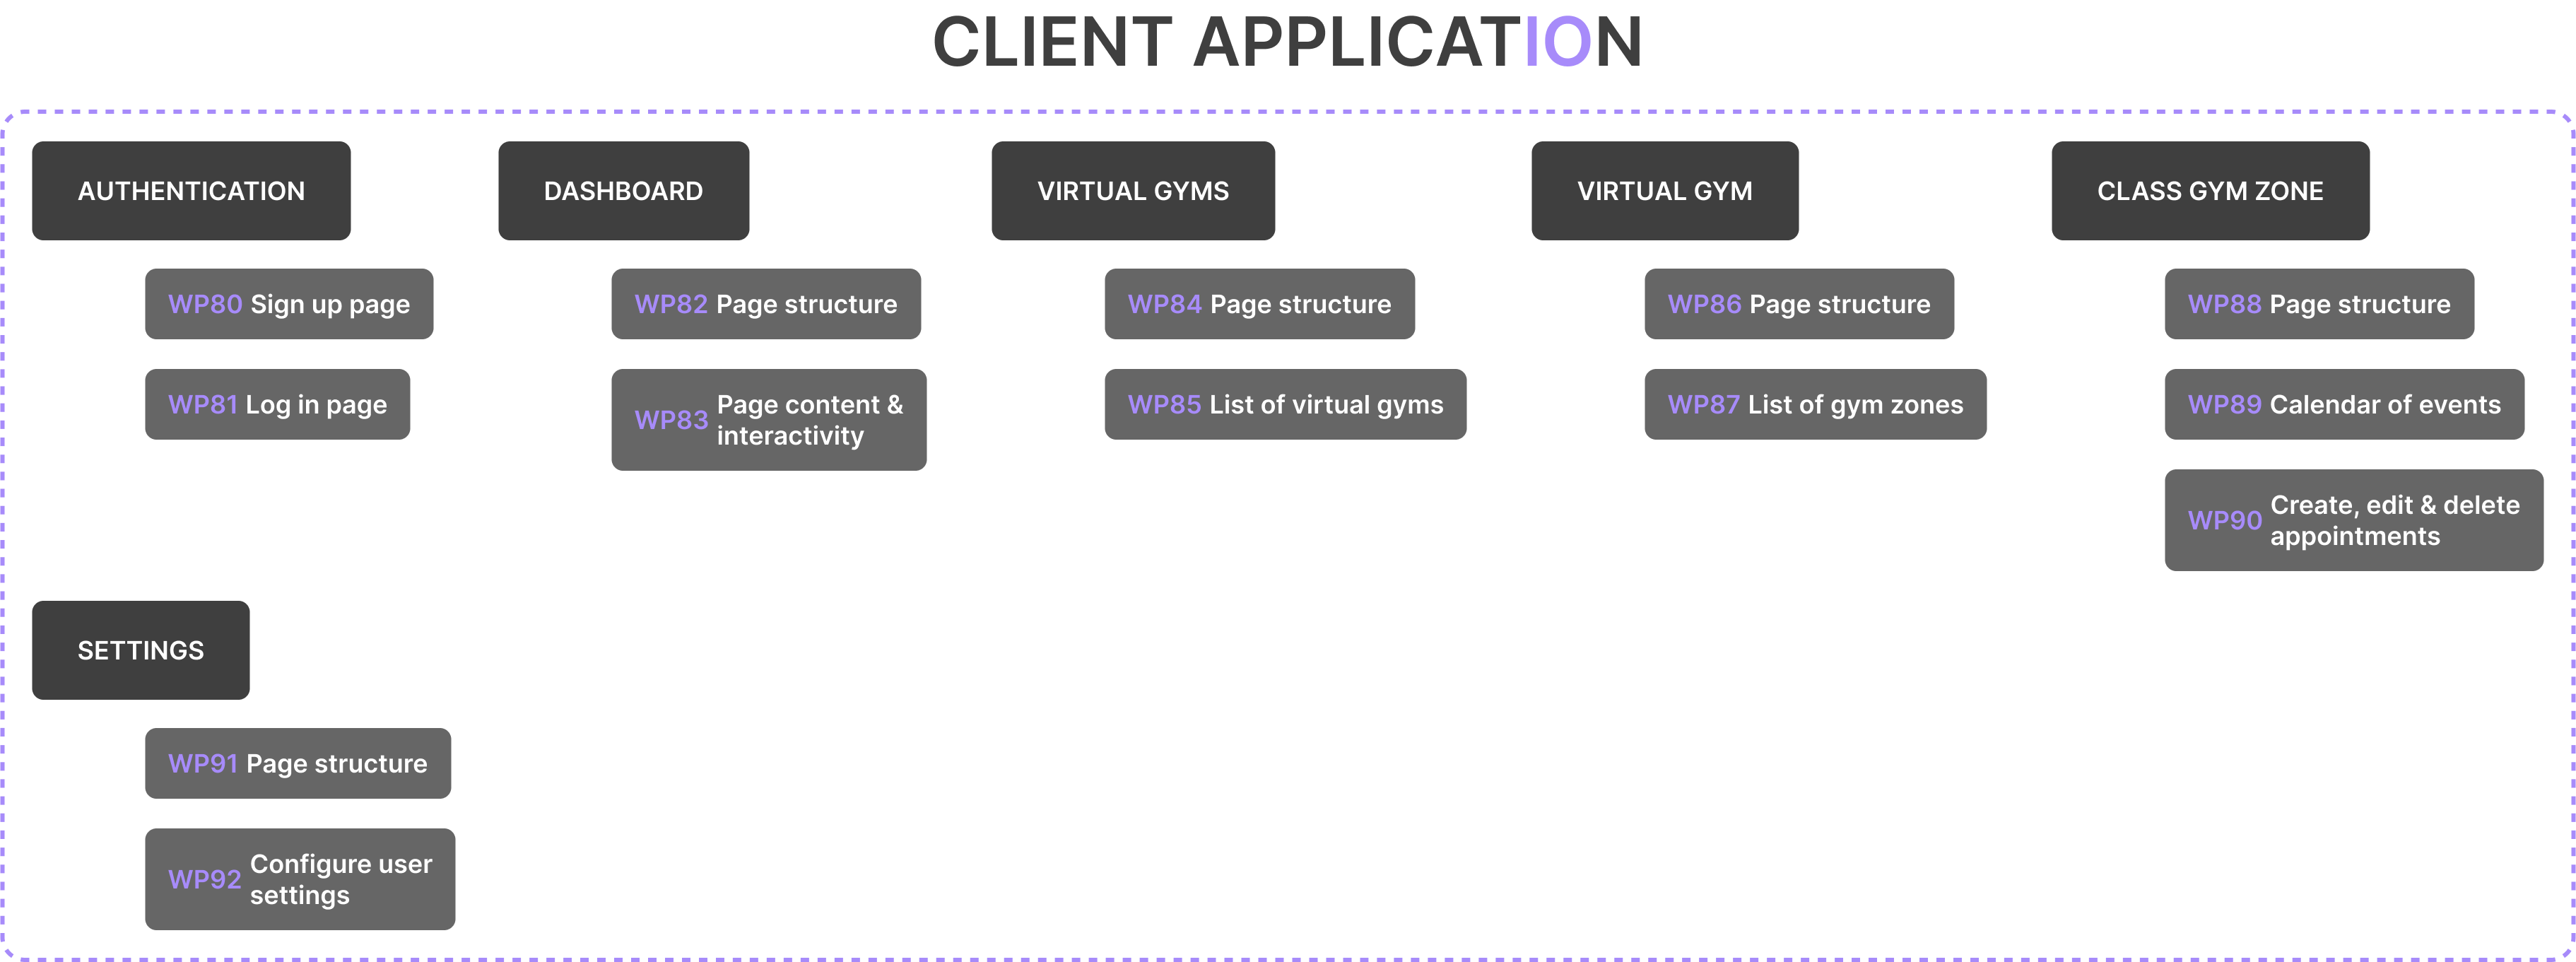
\includegraphics[width=\textwidth]{assets/working-packages/Client.png}
	\caption{Client application working packages diagram}
\end{figure}
The \emph{client} group is composed of the following working packages:
\\[8pt]
\begin{tabularx}{\textwidth}{| l | X |}
	\hline
	\rowcolor{rowColor}
	{\semibf Package name}   & {\semibf WP80}: Sign up page                 \\
	\hline
	{\semibf Description}    & Develop the sign up page                     \\
	\hline
	\rowcolor{rowColor}
	{\semibf Estimated time} & 8h                                           \\
	\hline
	{\semibf Tasks}          & {\semibf T1}: Set up the page structure.
	\newline {\semibf T2}: Sign up as a client.                             \\
	\hline
	\rowcolor{rowColor}
	{\semibf Results}        & Allow the clients to register to the system. \\
	\hline
\end{tabularx}
\captionof{table}{Package eighty's table - Sign up page}
\vspace*{16pt}
\begin{tabularx}{\textwidth}{| l | X |}
	\hline
	\rowcolor{rowColor}
	{\semibf Package name}   & {\semibf WP81}: Log in page              \\
	\hline
	{\semibf Description}    & Develop the log in page.                 \\
	\hline
	\rowcolor{rowColor}
	{\semibf Estimated time} & 8h                                       \\
	\hline
	{\semibf Tasks}          & {\semibf T1}: Set up the page structure.
	\newline {\semibf T2}: Log in as a client.                          \\
	\hline
	\rowcolor{rowColor}
	{\semibf Results}        & Allow the user to log in to the system.  \\
	\hline
\end{tabularx}
\captionof{table}{Package eighty-one's table - Log in page}
\vspace*{16pt}
\begin{tabularx}{\textwidth}{| l | X |}
	\hline
	\rowcolor{rowColor}
	{\semibf Package name}   & {\semibf WP82}: Page structure (Dashboard)            \\
	\hline
	{\semibf Description}    & Apply the design of the dashboard page.               \\
	\hline
	\rowcolor{rowColor}
	{\semibf Estimated time} & 4h                                                    \\
	\hline
	{\semibf Tasks}          & {\semibf T1}: Apply the design of the dashboard page. \\
	\hline
	\rowcolor{rowColor}
	{\semibf Results}        & The scaffolding of the dashboard page.                \\
	\hline
\end{tabularx}
\captionof{table}{Package eighty-two's table - Page structure (Dashboard)}
\vspace*{16pt}
\begin{tabularx}{\textwidth}{| l | X |}
	\hline
	\rowcolor{rowColor}
	{\semibf Package name}   & {\semibf WP83}: Page content and interactivity (Dashboard) \\
	\hline
	{\semibf Description}    & Add the interactivity to the dashboard page.               \\
	\hline
	\rowcolor{rowColor}
	{\semibf Estimated time} & 6h                                                         \\
	\hline
	{\semibf Tasks}          & {\semibf T1}: Add virtual gyms' interactivity.
	\newline {\semibf T2}: Add gym zones' interactivity.                                  \\
	\hline
	\rowcolor{rowColor}
	{\semibf Results}        & User experience of the dasboard page.                      \\
	\hline
\end{tabularx}
\captionof{table}{Package eighty-three's table - Page content and interactivity}
\vspace*{16pt}
\begin{tabularx}{\textwidth}{| l | X |}
	\hline
	\rowcolor{rowColor}
	{\semibf Package name}   & {\semibf WP84}: Page structure (Virtual gyms)                            \\
	\hline
	{\semibf Description}    & Apply the design of the virtual gyms page. Should reuse the core's page. \\
	\hline
	\rowcolor{rowColor}
	{\semibf Estimated time} & 2h                                                                       \\
	\hline
	{\semibf Tasks}          & {\semibf T1}: Apply the design of the virtual gyms page.                 \\
	\hline
	\rowcolor{rowColor}
	{\semibf Results}        & The scaffolding of the virtual gyms page.                                \\
	\hline
\end{tabularx}
\captionof{table}{Package eighty-fourt's table - Page structure (Virtual gyms)}
\vspace*{16pt}
\begin{tabularx}{\textwidth}{| l | X |}
	\hline
	\rowcolor{rowColor}
	{\semibf Package name}   & {\semibf WP85}: List of virtual gyms (Virtual gyms) \\
	\hline
	{\semibf Description}    & Display the list of virtual gyms.                   \\
	\hline
	\rowcolor{rowColor}
	{\semibf Estimated time} & 2h                                                  \\
	\hline
	{\semibf Tasks}          & {\semibf T1}: List the virtual gyms of the gym.
	\newline {\semibf T2}: List the gym zones inside each virtual gym.             \\
	\hline
	\rowcolor{rowColor}
	{\semibf Results}        & The page of virtual gyms.                           \\
	\hline
\end{tabularx}
\captionof{table}{Package eighty-five's table - List of virtual gyms (Virtual gyms)}
\vspace*{16pt}
\begin{tabularx}{\textwidth}{| l | X |}
	\hline
	\rowcolor{rowColor}
	{\semibf Package name}   & {\semibf WP86}: Page structure (Virtual gym)                            \\
	\hline
	{\semibf Description}    & Apply the design of the virtual gym page. Should reuse the core's page. \\
	\hline
	\rowcolor{rowColor}
	{\semibf Estimated time} & 2h                                                                      \\
	\hline
	{\semibf Tasks}          & {\semibf T1}: Apply the design of the virtual gym page.                 \\
	\hline
	\rowcolor{rowColor}
	{\semibf Results}        & The scaffolding of the virtual gym page.                                \\
	\hline
\end{tabularx}
\captionof{table}{Package eighty-six's table - Page structure (Virtual gym)}
\vspace*{16pt}
\begin{tabularx}{\textwidth}{| l | X |}
	\hline
	\rowcolor{rowColor}
	{\semibf Package name}   & {\semibf WP87}: List of gym zones (Virtual gym) \\
	\hline
	{\semibf Description}    & List the gym zones of a virtual gym.            \\
	\hline
	\rowcolor{rowColor}
	{\semibf Estimated time} & 2h                                              \\
	\hline
	{\semibf Tasks}          & {\semibf T1}: List all class gym zones.
	\newline {\semibf T2}: List all non-class gym zones.                       \\
	\hline
	\rowcolor{rowColor}
	{\semibf Results}        & The page of a virtual gym.                      \\
	\hline
\end{tabularx}
\captionof{table}{Package eighty-seven's table - List of gym zones (Virtual gym)}
\vspace*{16pt}
\begin{tabularx}{\textwidth}{| l | X |}
	\hline
	\rowcolor{rowColor}
	{\semibf Package name}   & {\semibf WP88}: Page structure (Class gym zone)                            \\
	\hline
	{\semibf Description}    & Apply the design of the class gym zone page. Should reuse the core's page. \\
	\hline
	\rowcolor{rowColor}
	{\semibf Estimated time} & 2h                                                                         \\
	\hline
	{\semibf Tasks}          & {\semibf T1}: Apply the design of the class gym zone page.                 \\
	\hline
	\rowcolor{rowColor}
	{\semibf Results}        & The scaffolding of the class gym zone page.                                \\
	\hline
\end{tabularx}
\captionof{table}{Package eighty-eight's table - Page structure (Class gym zone)}
\vspace*{16pt}
\begin{tabularx}{\textwidth}{| l | X |}
	\hline
	\rowcolor{rowColor}
	{\semibf Package name}   & {\semibf WP89}: Calendar of events (Class gym zone) \\
	\hline
	{\semibf Description}    & Display the calendar of events of the gym zone.     \\
	\hline
	\rowcolor{rowColor}
	{\semibf Estimated time} & 4h                                                  \\
	\hline
	{\semibf Tasks}          & {\semibf T1}: Design the calendar of events.
	{\semibf T2}: Add interactivity to the calendar.                               \\
	\hline
	\rowcolor{rowColor}
	{\semibf Results}        & The calendar of events for the gym zone.            \\
	\hline
\end{tabularx}
\captionof{table}{Package ninety's table - Calendar of events (Class gym zone)}
\vspace*{16pt}
\begin{tabularx}{\textwidth}{| l | X |}
	\hline
	\rowcolor{rowColor}
	{\semibf Package name}   & {\semibf WP90}: Create, edit and delete appointments (Class gym zone) \\
	\hline
	{\semibf Description}    & Modal to create, edit and delete appointments.                        \\
	\hline
	\rowcolor{rowColor}
	{\semibf Estimated time} & 8h                                                                    \\
	\hline
	{\semibf Tasks}          & {\semibf T1}: Modal to create, edit and delete appointments.          \\
	\hline
	\rowcolor{rowColor}
	{\semibf Results}        & The modal to interact with appointments.                              \\
	\hline
\end{tabularx}
\captionof{table}{Package ninety's table - Create, edit and delete appointments (Class gym zone)}
\vspace*{16pt}
\begin{tabularx}{\textwidth}{| l | X |}
	\hline
	\rowcolor{rowColor}
	{\semibf Package name}   & {\semibf WP91}: Page structure (Settings)                            \\
	\hline
	{\semibf Description}    & Apply the design of the settings page. Should reuse the core's page. \\
	\hline
	\rowcolor{rowColor}
	{\semibf Estimated time} & 2h                                                                   \\
	\hline
	{\semibf Tasks}          & {\semibf T1}: Apply the design of the settings page.                 \\
	\hline
	\rowcolor{rowColor}
	{\semibf Results}        & The scaffolding of the settings page.                                \\
	\hline
\end{tabularx}
\captionof{table}{Package ninety-one's table - Page structure (Settings)}
\vspace*{16pt}
\begin{tabularx}{\textwidth}{| l | X |}
	\hline
	\rowcolor{rowColor}
	{\semibf Package name}   & {\semibf WP92}: Configure user settings (Settings) \\
	\hline
	{\semibf Description}    & Set up the form to update client settings.         \\
	\hline
	\rowcolor{rowColor}
	{\semibf Estimated time} & 4h                                                 \\
	\hline
	{\semibf Tasks}          & {\semibf T1}: Log out the client.
	\newline {\semibf T2}: Configure the basic fields of the client.
	\newline {\semibf T3}: Update the client password.                            \\
	\hline
	\rowcolor{rowColor}
	{\semibf Results}        & The settings page.                                 \\
	\hline
\end{tabularx}
\captionof{table}{Package ninety-two's table - Configure user settings (Settings)}
\subsubsection{Landing application}
The landing application is a simple application that displays information about the system and acces to the main application.
\begin{tabularx}{\textwidth}{| l | X |}
	\hline
	\rowcolor{rowColor}
	{\semibf Package name}   & {\semibf WP93}: Design the landing application            \\
	\hline
	{\semibf Description}    & Set up the form to update client settings.                \\
	\hline
	\rowcolor{rowColor}
	{\semibf Estimated time} & 16h                                                        \\
	\hline
	{\semibf Tasks}          & {\semibf T1}: Display basic information about the system.
	\newline {\semibf T2}: Display information about the data privacy.
	\newline {\semibf T3}: Display a contact form.                                       \\
	\hline
	\rowcolor{rowColor}
	{\semibf Results}        & The landing application.                                  \\
	\hline
\end{tabularx}
\captionof{table}{Package ninety-three's table - Landing page}
% endregion PLANNING_TABLES
\section{Traceability matrix}
Due to the large quantity of requirements and working packageds that have been determined for the development of the project, and due to the low relationship between them, the traceability matrix will be shown individually, in order to avoid displaying a nearly empty table. Using the following notation, the result is more consise and can be understood better.
\\[8pt]
Each dependency will use the following format: [FR-1] \texttt{->} [WP-1, WP-2, WP-3]. It states that the functional requirements 1 will be covered in the working package 1, 2 and 3.
\begin{enumerate}[label = -]
	\item {[FR-1, FR-2, FR-3, FR-4] \texttt{->} [WP-93]}
	\item {[FR-5, FR-6] \texttt{->} [WP-51]}
	\item {[FR-7] \texttt{->} [WP-52]}
	\item {[FR-8, FR-9, FR-10] \texttt{->} [WP-93]}
	\item {[FR-11, FR-13, FR-14, FR-15, FR-17] \texttt{->} [WP-56, WP-28, WP-29, WP-30]}
	\item {[FR-12, FR-16] \texttt{->} [WP-57, WP-27, WP-28, WP-29]}
	\item {[FR-19, FR-21, FR-22] \texttt{->} [WP-59, WP-34]}
	\item {[FR-20, FR-23] \texttt{->} [WP-60, WP-31, WP-32, WP-33]}
	\item {[FR-24, FR-27, FR-28] \texttt{->} [WP-62, WP-43, WP-44, WP-45, WP-47, WP-48, WP-49]}
	\item {[FR-25, FR-26, FR-29, FR-30] \texttt{->} [WP-63, WP-34, WP-46, WP-50]}
	\item {[FR-31, FR-33] \texttt{->} [WP-66, WP-38, WP-42, WP-46]}
	\item {[FR-32, FR-35] \texttt{->} [WP-67, WP-35, WP-36, WP-37]}
	\item {[FR-34, FR-36] \texttt{->} [WP-68, WP-39, WP-40, WP-41]}
	\item {[FR-37, FR-38, FR-40] \texttt{->} [WP-74, WP-19, WP-20, WP-21]}
	\item {[FR-39, FR-41] \texttt{->} [WP-73, WP-22]}
	\item {[FR-42, FR-43, FR-45] \texttt{->} [WP-70, WP-23, WP-24, WP-25]}
	\item {[FR-44, FR-46] \texttt{->} [WP-71, WP-26]}
	\item {[FR-47, FR-48] \texttt{->} [WP-77]}
	\item {[FR-49, FR-50] \texttt{->} [WP-76]}
	\item {[FR-51, FR-52, FR-53, FR-54, FR-55, FR-56] \texttt{->} [WP-79, WP-17]}
	\item {[FR-65] \texttt{->} [WP-80, WP-16]}
	\item {[FR-66] \texttt{->} [WP-81, WP-17]}
	\item {[FR-67, FR-68] \texttt{->} [WP-85, WP-30]}
	\item {[FR-69] \texttt{->} [WP-89, WP-46]}
	\item {[FR-70, FR-71, FR-72] \texttt{->} [WP-90, WP-43, WP-44, WP-45, WP-47, WP-48, WP-49]}
	\item {[FR-73, FR-74, FR-75, FR-76, FR-77, FR-78] \texttt{->} [WP-92, WP-17]}
	\item {[NFR-1] \texttt{->} [WP-16, WP-18]}
	\item {[NFR-2] \texttt{->} [WP-52]}
	\item {[NFR-3] \texttt{->} [WP-93]}
	\item {[NFR-4] \texttt{->} [WP-53, WP-55, WP-58, WP-61, WP-65, WP-69, WP-72, WP-75, WP-78]}
	\item {[NFR-5] \texttt{->} [WP-53, WP-55, WP-58, WP-61, WP-65, WP-69, WP-72, WP-75, WP-78, WP-82, WP-84, WP-86, WP-88, WP-91, WP-93]}
\end{enumerate}
\section{User interfaces}
The design of the user interfaces has been a priority before diving into the front end development. Such interfices, provide a preliminar view of what show the application look and feel. The following figures, are the designs of the user interfaces that have been designed using the Figma software\footnote{The figma application is a free software which can be found in: \href{www.figma.com}{www.figma.com}}.
\\
Designing every possible state of the application is far from achievable with such little time. However, since the core and client application will share much of their user interface, only the core views have been designed. When developing the client application, most of the components have been reused, modifying they behaviour as needed, since the client interactions are limited (for instance, the client sees the same dashboard page, yet the button to add a virtual gym is hidden). Needless to say, some views do not correspond exactly as they are in the application, mainly because some features have been modified or added as required.
\\
Finally, the following aspects have been considered when designing the views:
\begin{enumerate}[label = -]
	\item The views should also be displayed as an owner used. This is due to the fact that the only differences between the views of an owner, a worker or a client, will be minimal. Some things will be hidden or not allowed, which has little effects to the final design.
	\item Each element that can be created (virtual gyms, gym zones, trainers and so on) must have their corresponding dialog or view in which such items are created, edited or deleated.
	      \begin{enumerate}[label = -]
		      \item In case a dialog is used, it has to contain how it looks when: it is being created, it is being edited, and it is being loaded, for each of the previous states.
	      \end{enumerate}
\end{enumerate}
With these requirements, there are views modals that contain 4 images, each one for the described states.
\\
% region Images
\begin{figure}[H]
	\centering
	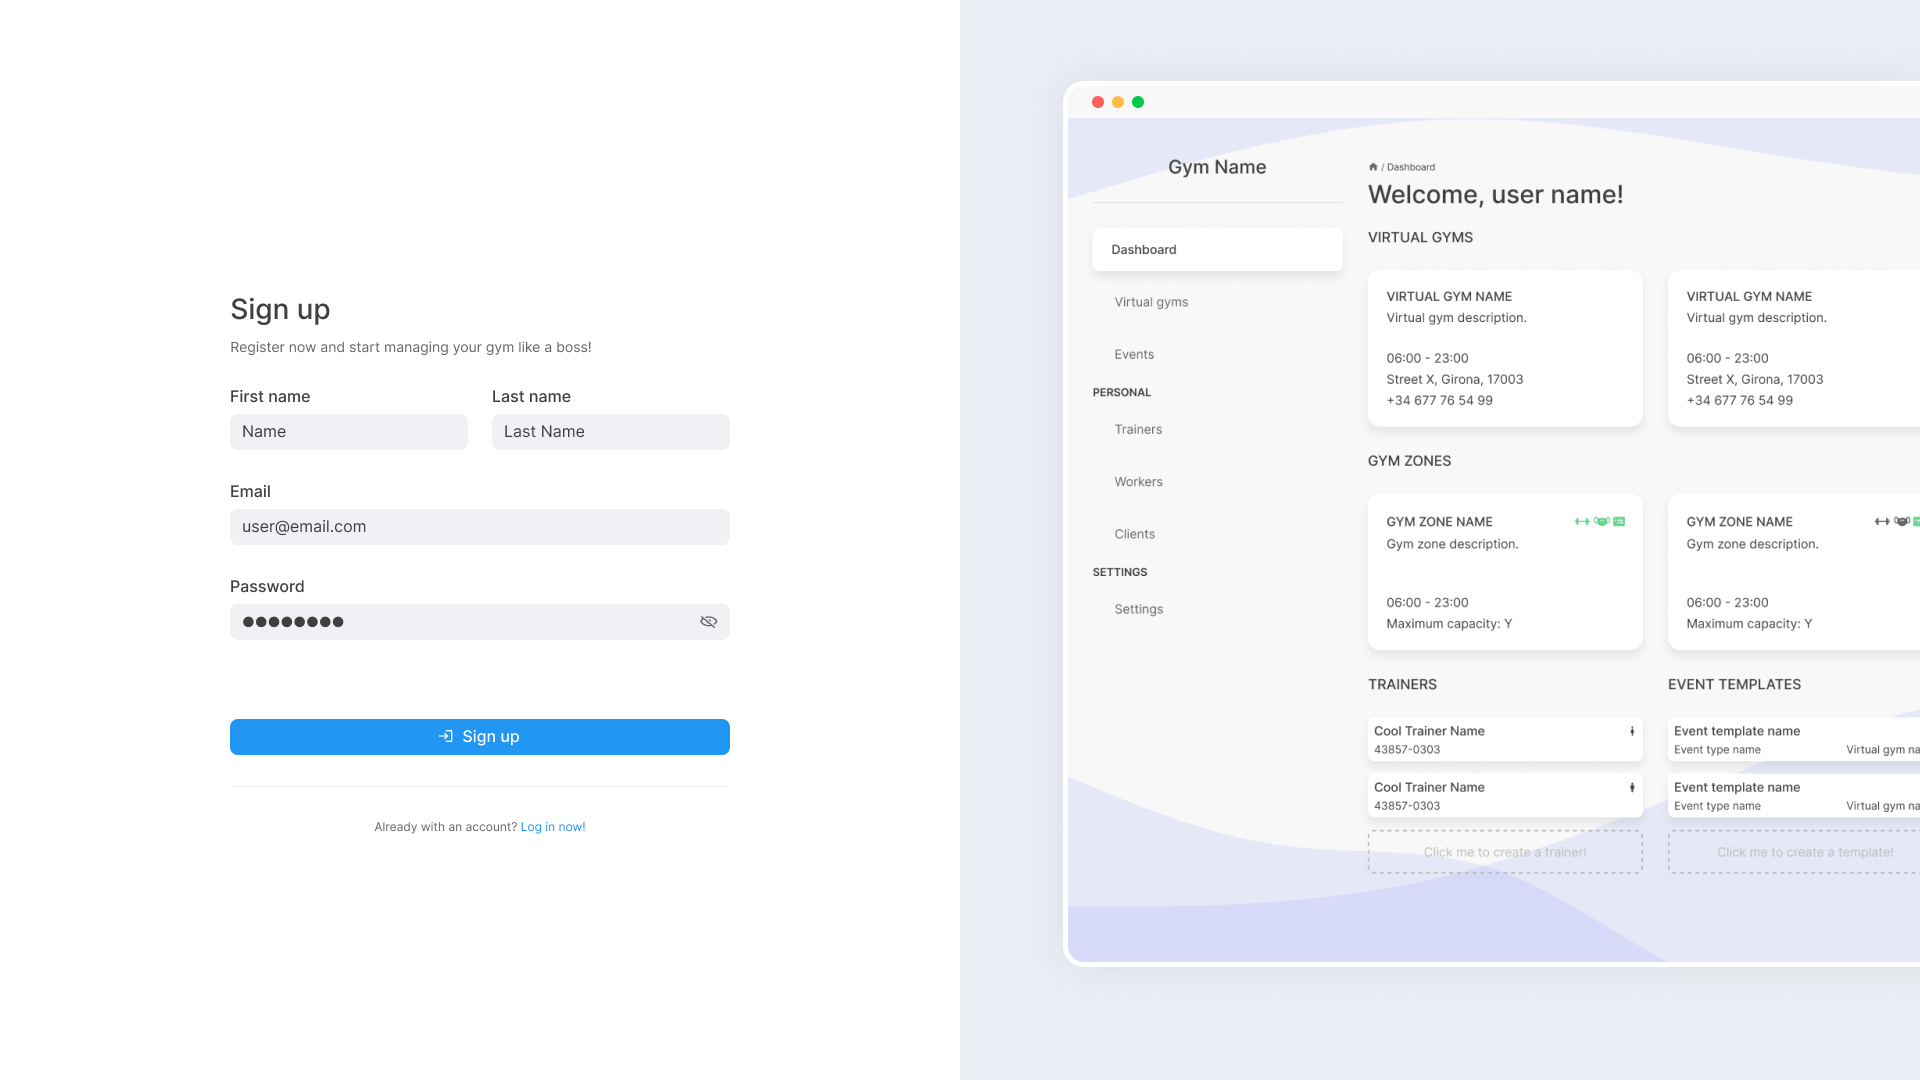
\includegraphics[width=\textwidth]{assets/ui/SignUpStepOne.png}
	\caption{First step of the sign up page}
\end{figure}
\begin{figure}[H]
	\centering
	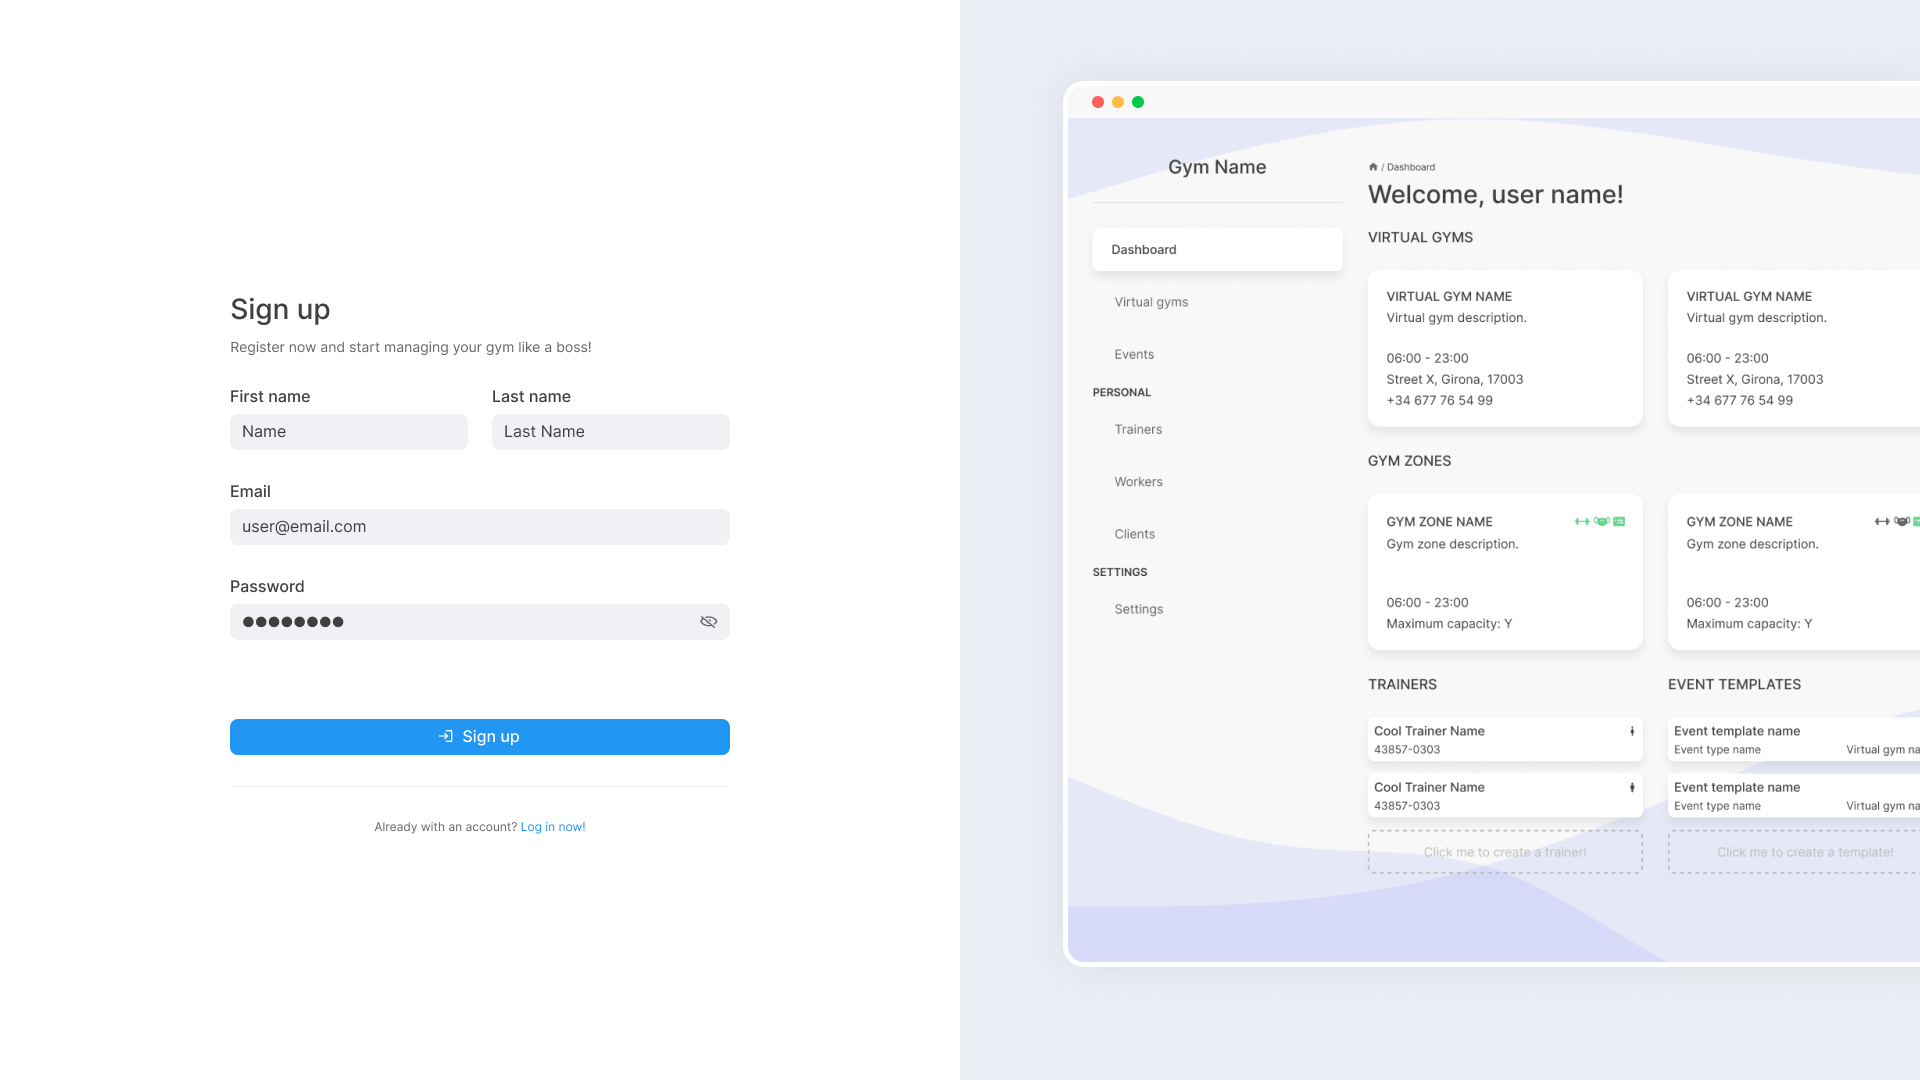
\includegraphics[width=\textwidth]{assets/ui/SignUpStepOne.png}
	\caption{Second step of the sign up page}
\end{figure}
\begin{figure}[H]
	\centering
	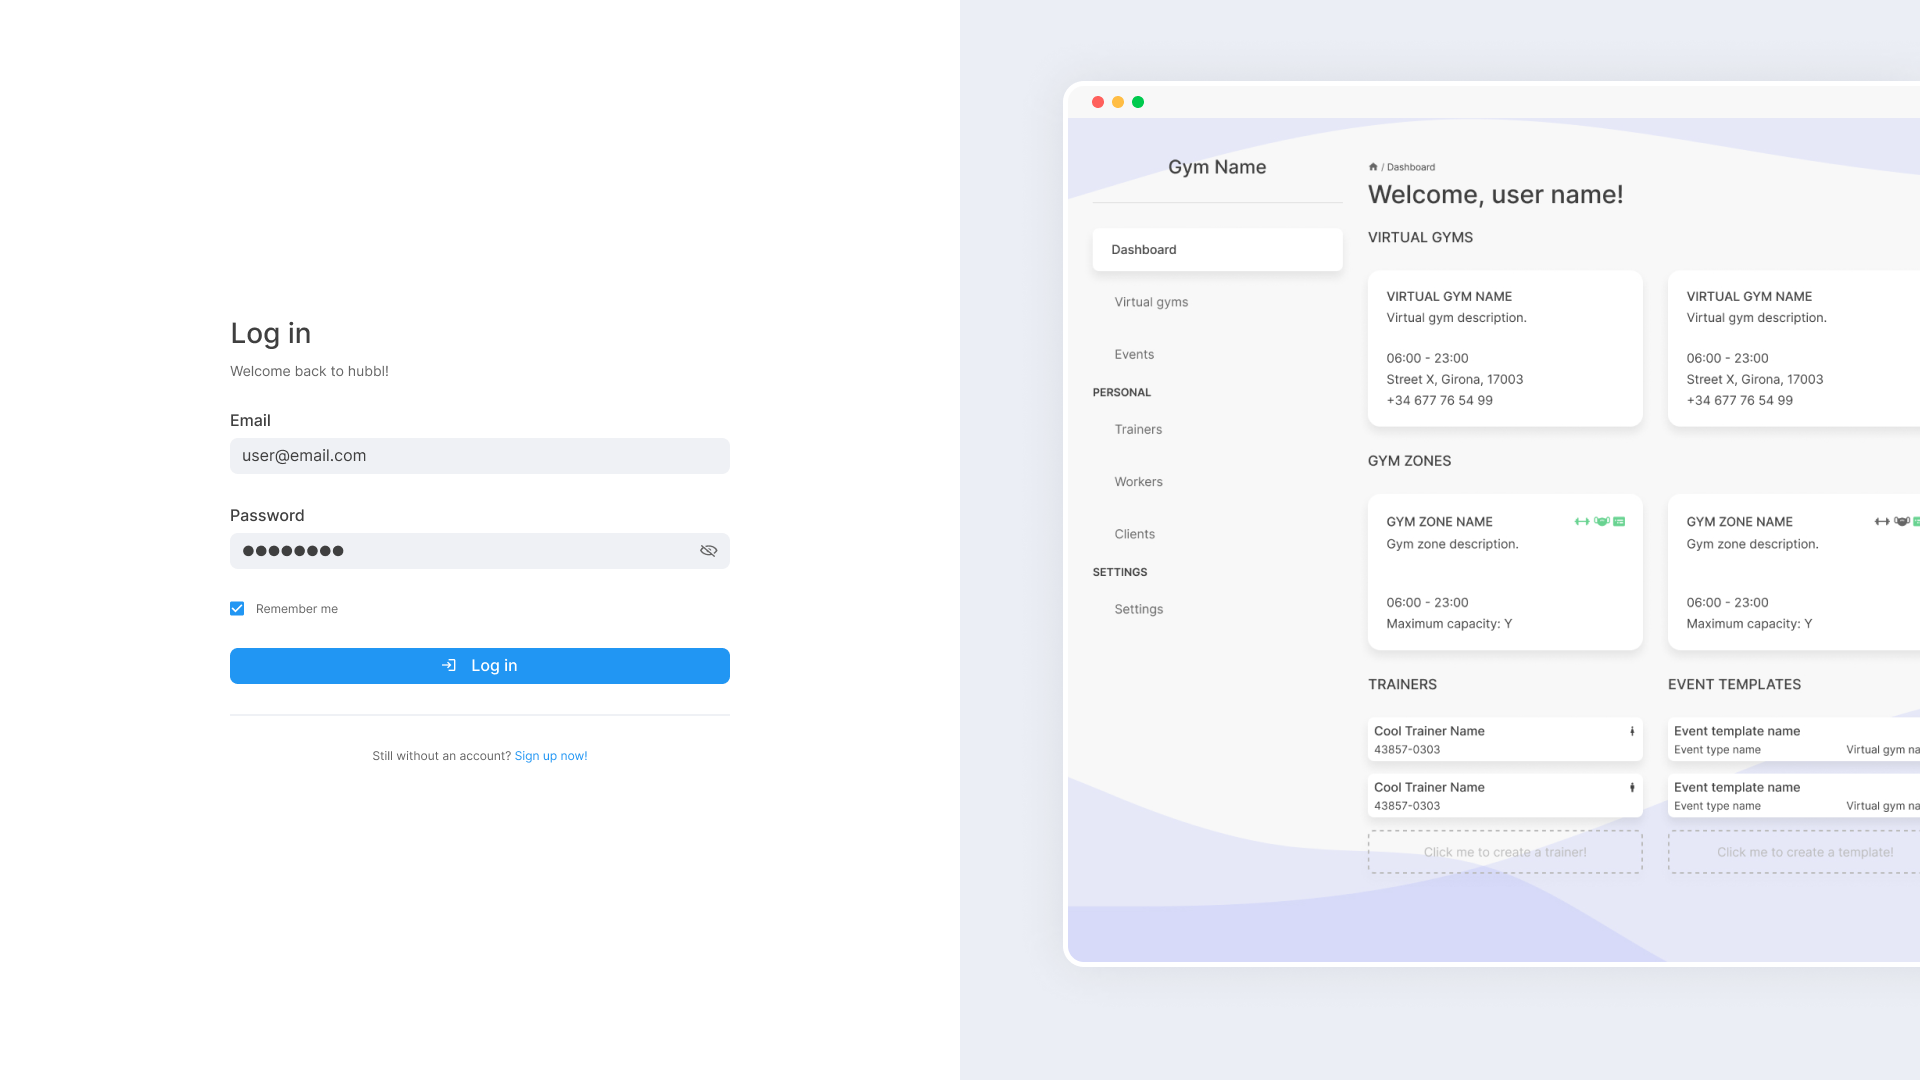
\includegraphics[width=\textwidth]{assets/ui/LogIn.png}
	\caption{View of the login page}
\end{figure}
\begin{figure}[H]
	\centering
	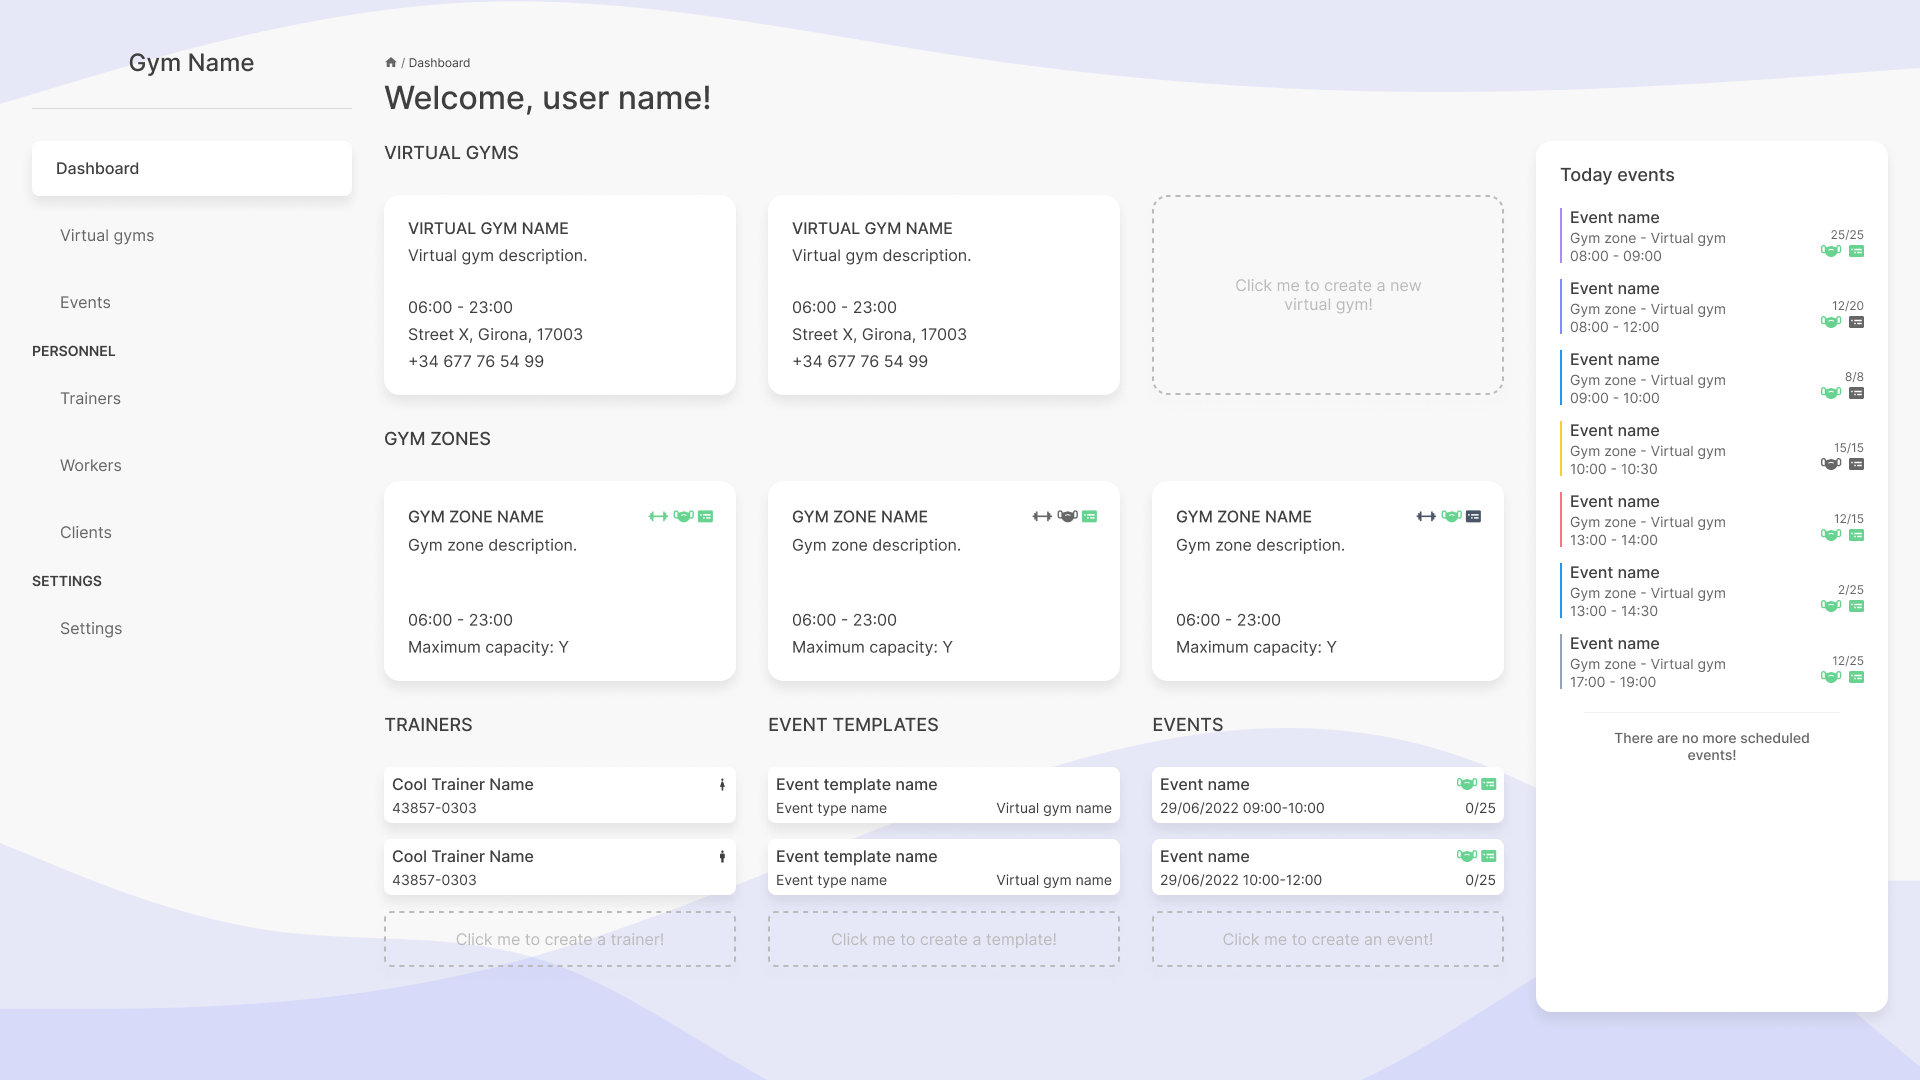
\includegraphics[width=\textwidth]{assets/ui/Dashboard.png}
	\caption{Dashboard page, displaying a summary of the gym's information}
\end{figure}
\begin{figure}[H]
	\centering
	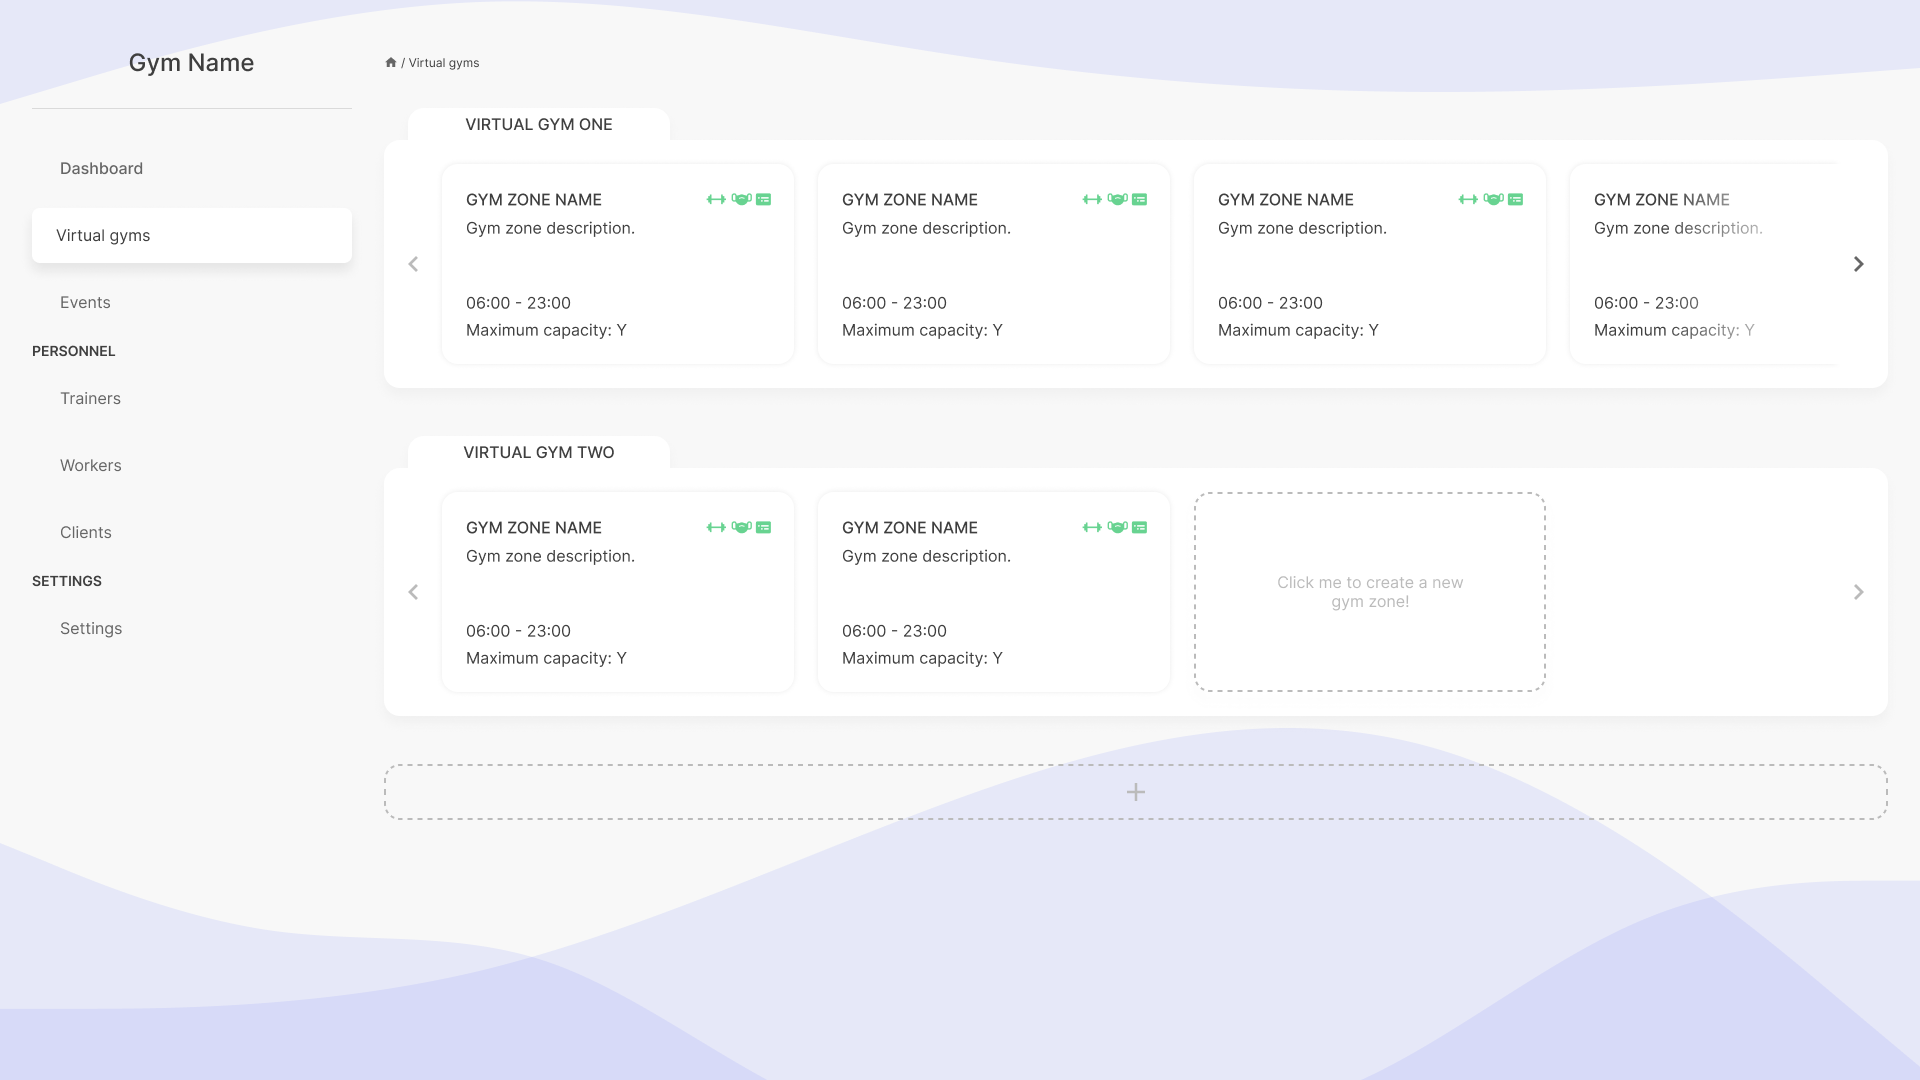
\includegraphics[width=\textwidth]{assets/ui/VirtualGyms.png}
	\caption{Virtual gym's page, which is accessed using the left navigation bar}
\end{figure}
\begin{figure}[H]
	\centering
	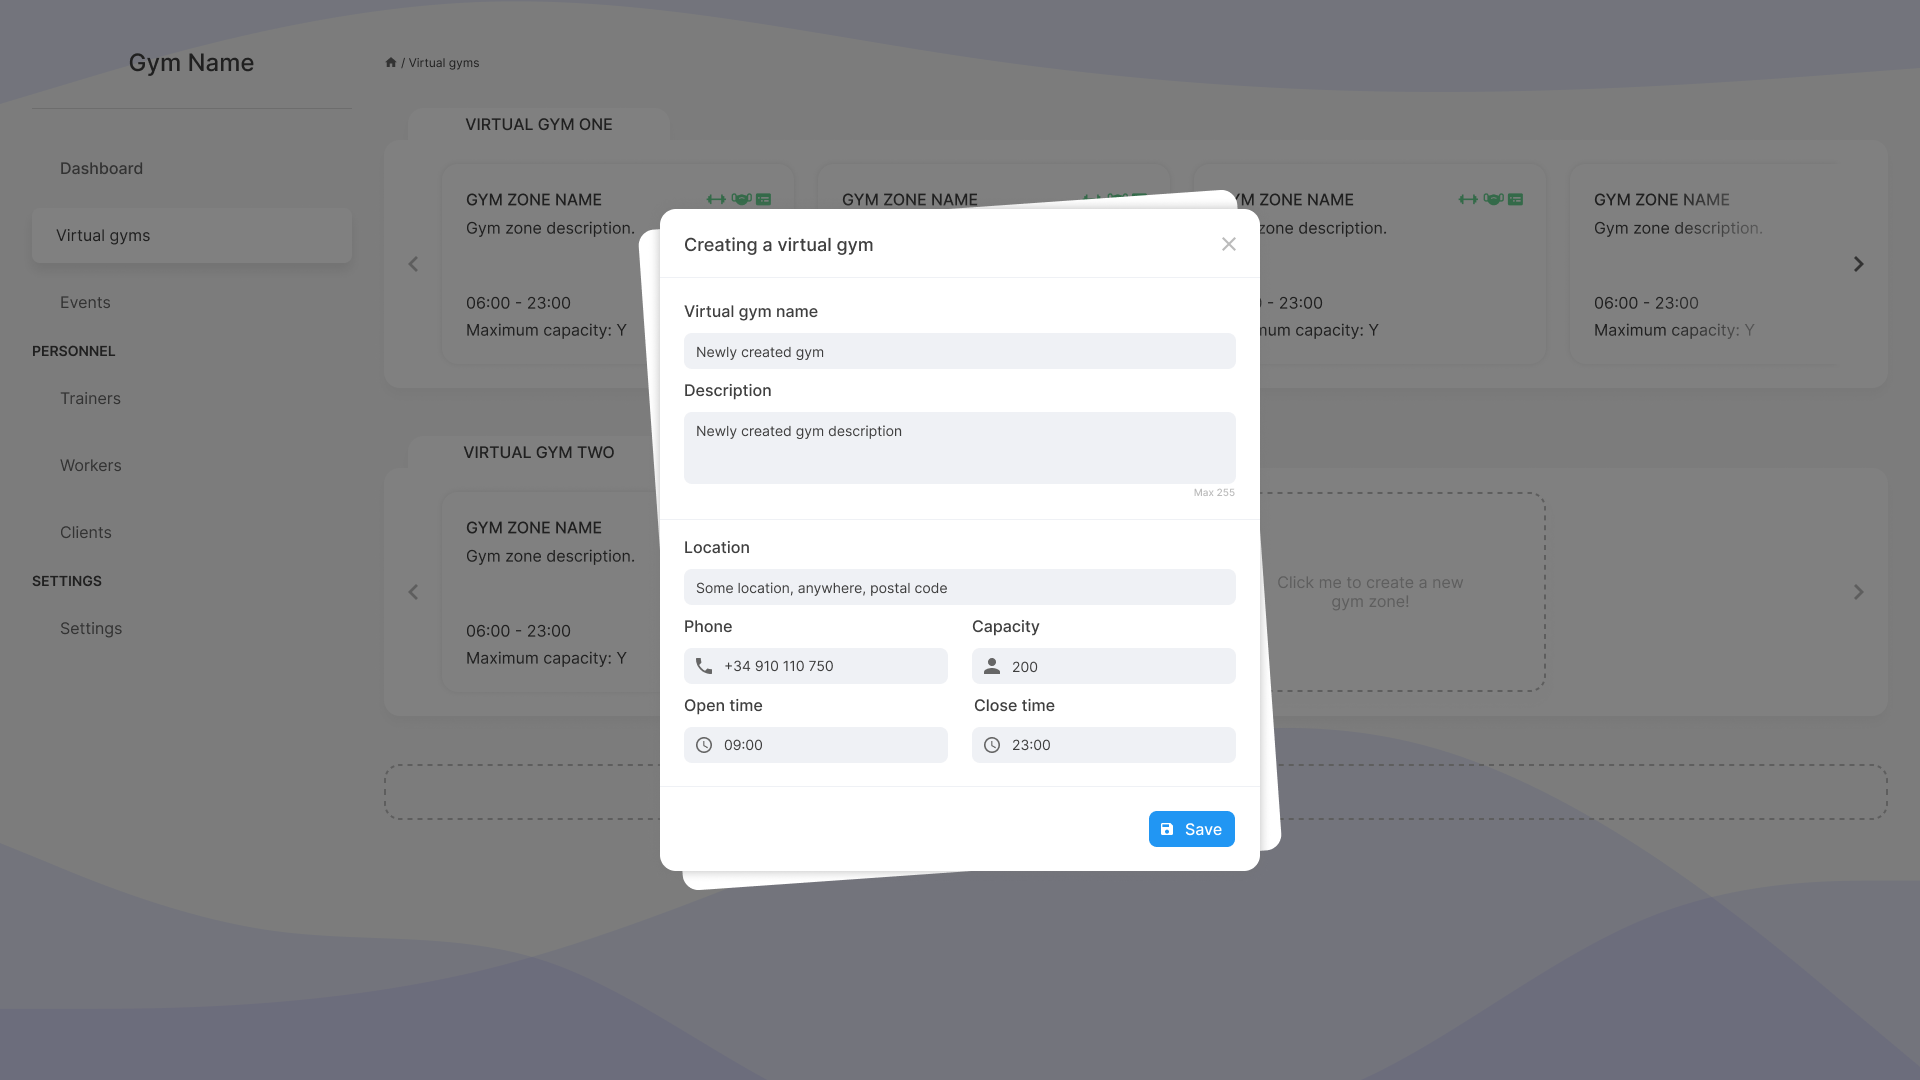
\includegraphics[width=\textwidth]{assets/ui/CreateVirtualGym.png}
	\caption{Virtual gym dialog (create state)}
\end{figure}
\begin{figure}[H]
	\centering
	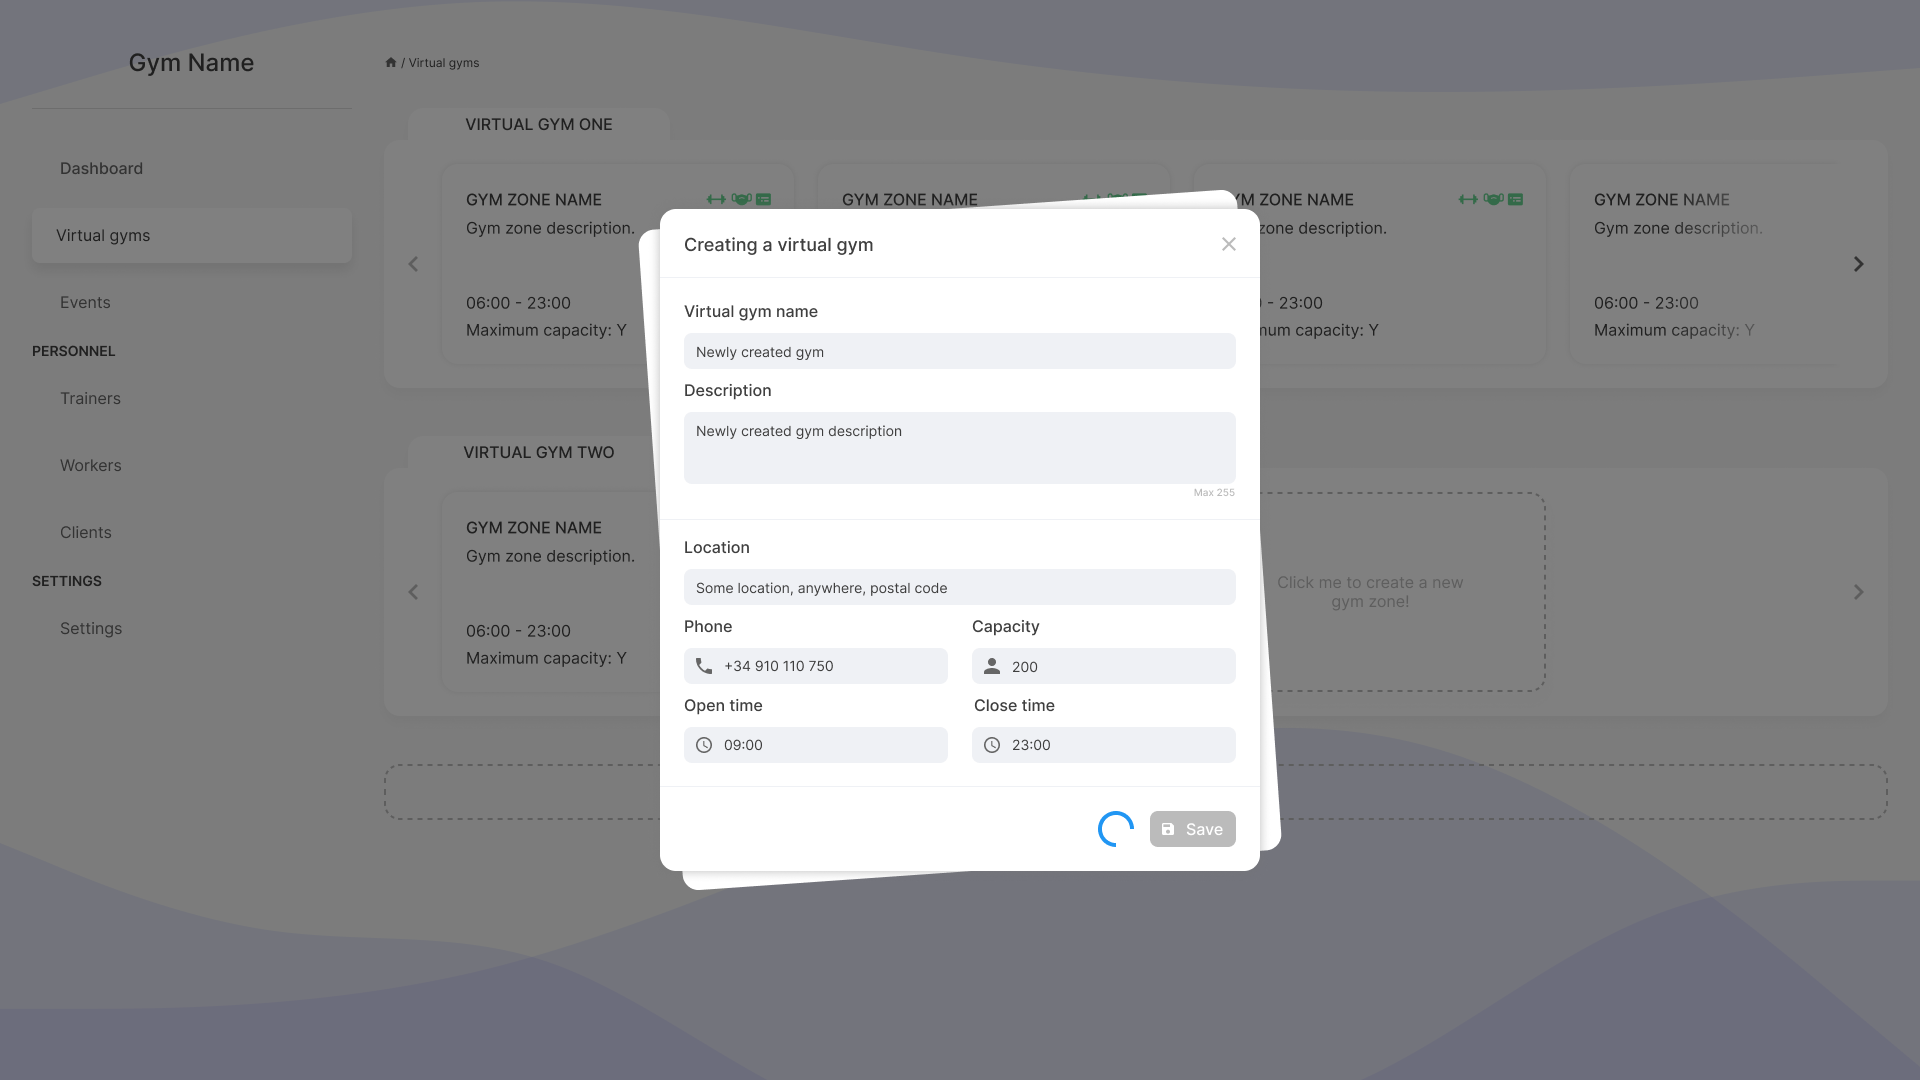
\includegraphics[width=\textwidth]{assets/ui/CreateLoadingVirtualGym.png}
	\caption{Virtual gym dialog (create-loading state)}
\end{figure}
\begin{figure}[H]
	\centering
	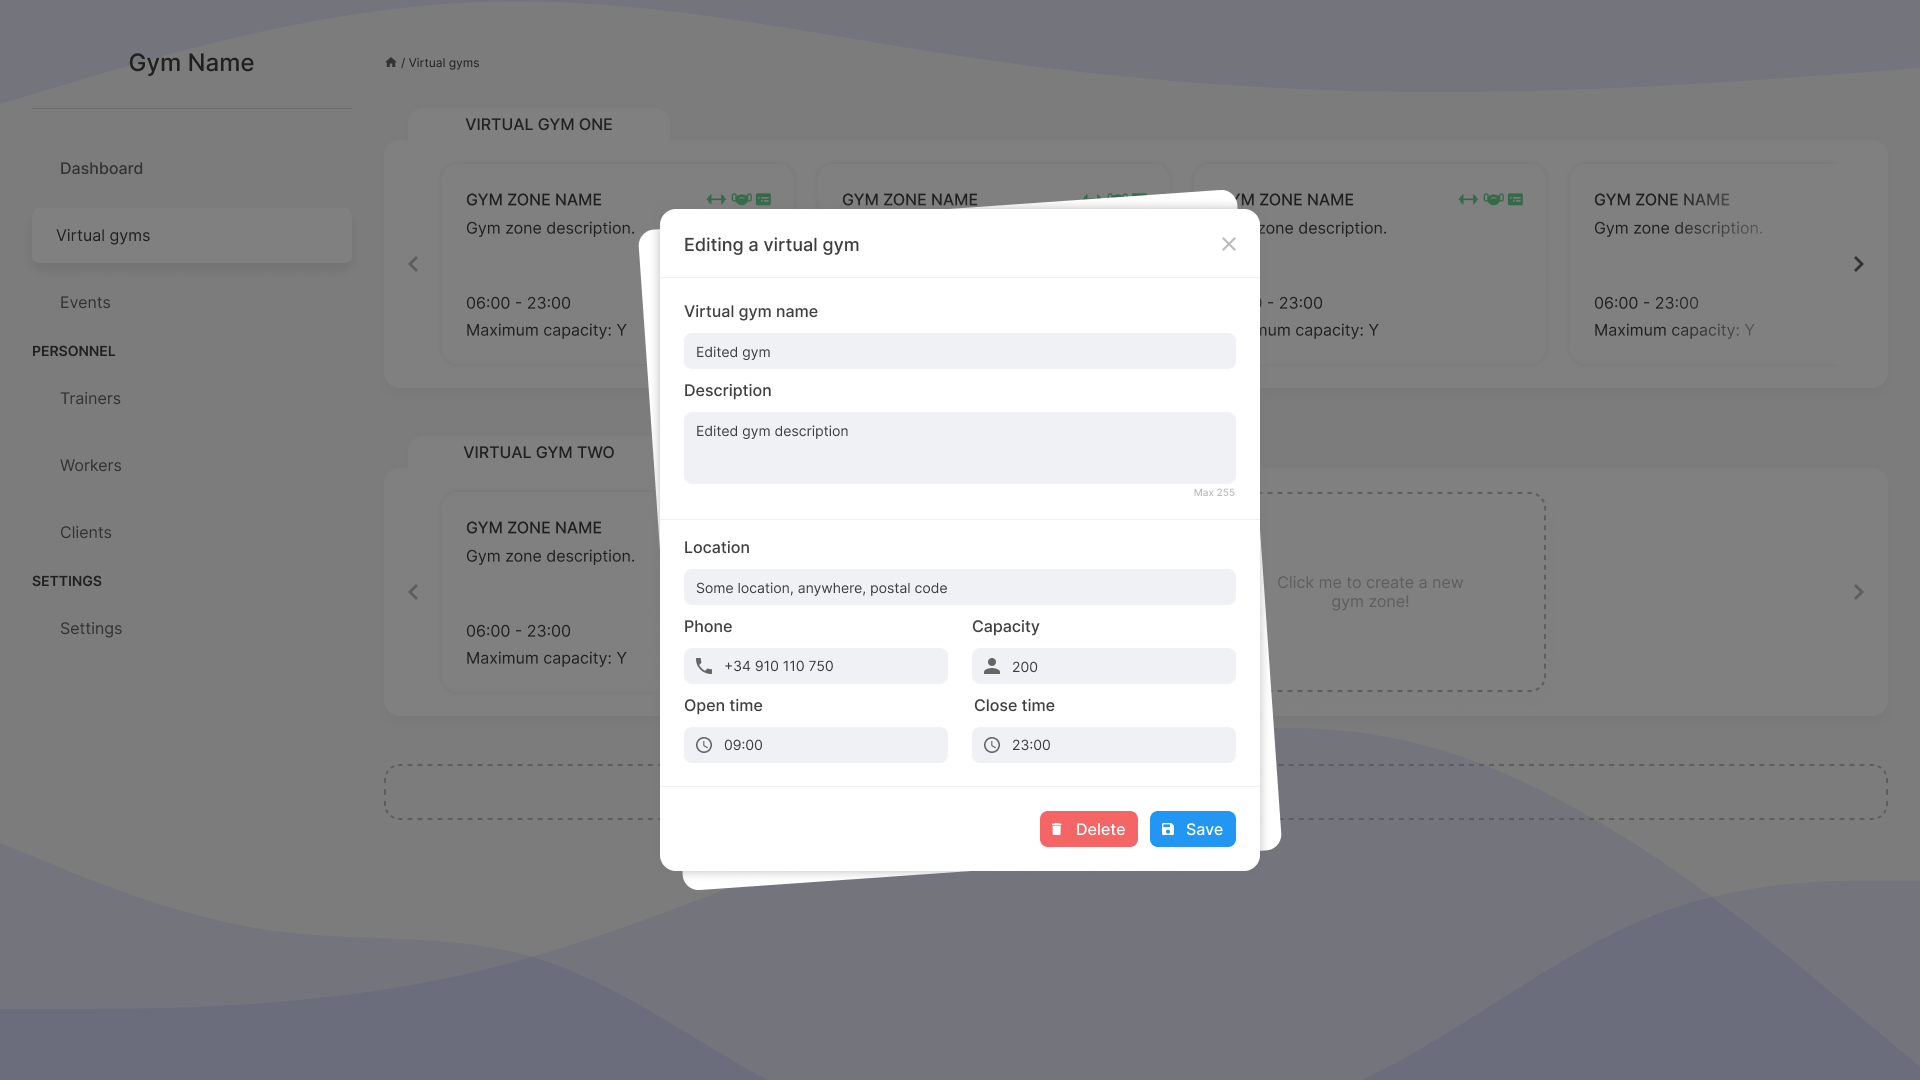
\includegraphics[width=\textwidth]{assets/ui/EditVirtualGym.png}
	\caption{Virtual gym dialog (edit state)}
\end{figure}
\begin{figure}[H]
	\centering
	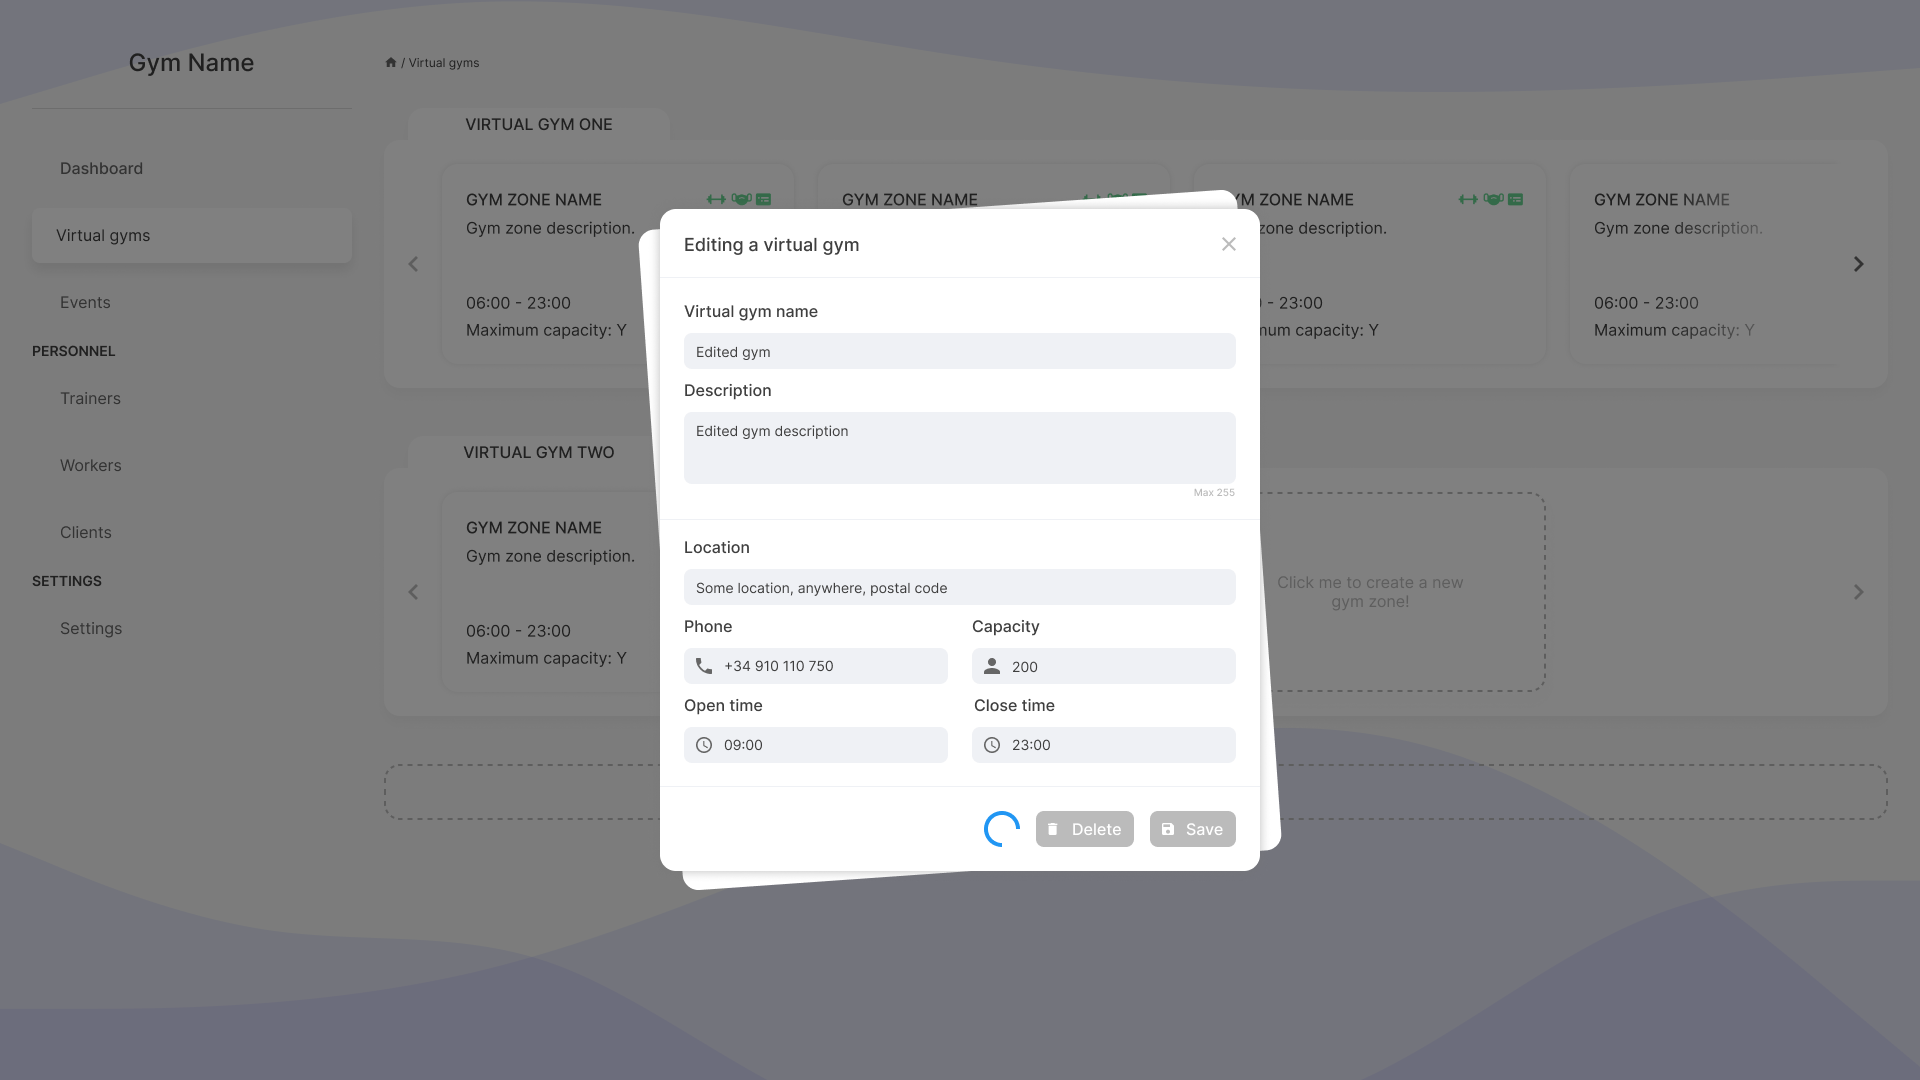
\includegraphics[width=\textwidth]{assets/ui/EditLoadingVirtualGym.png}
	\caption{Virtual gym dialog (edit-loading state)}
\end{figure}
\begin{figure}[H]
	\centering
	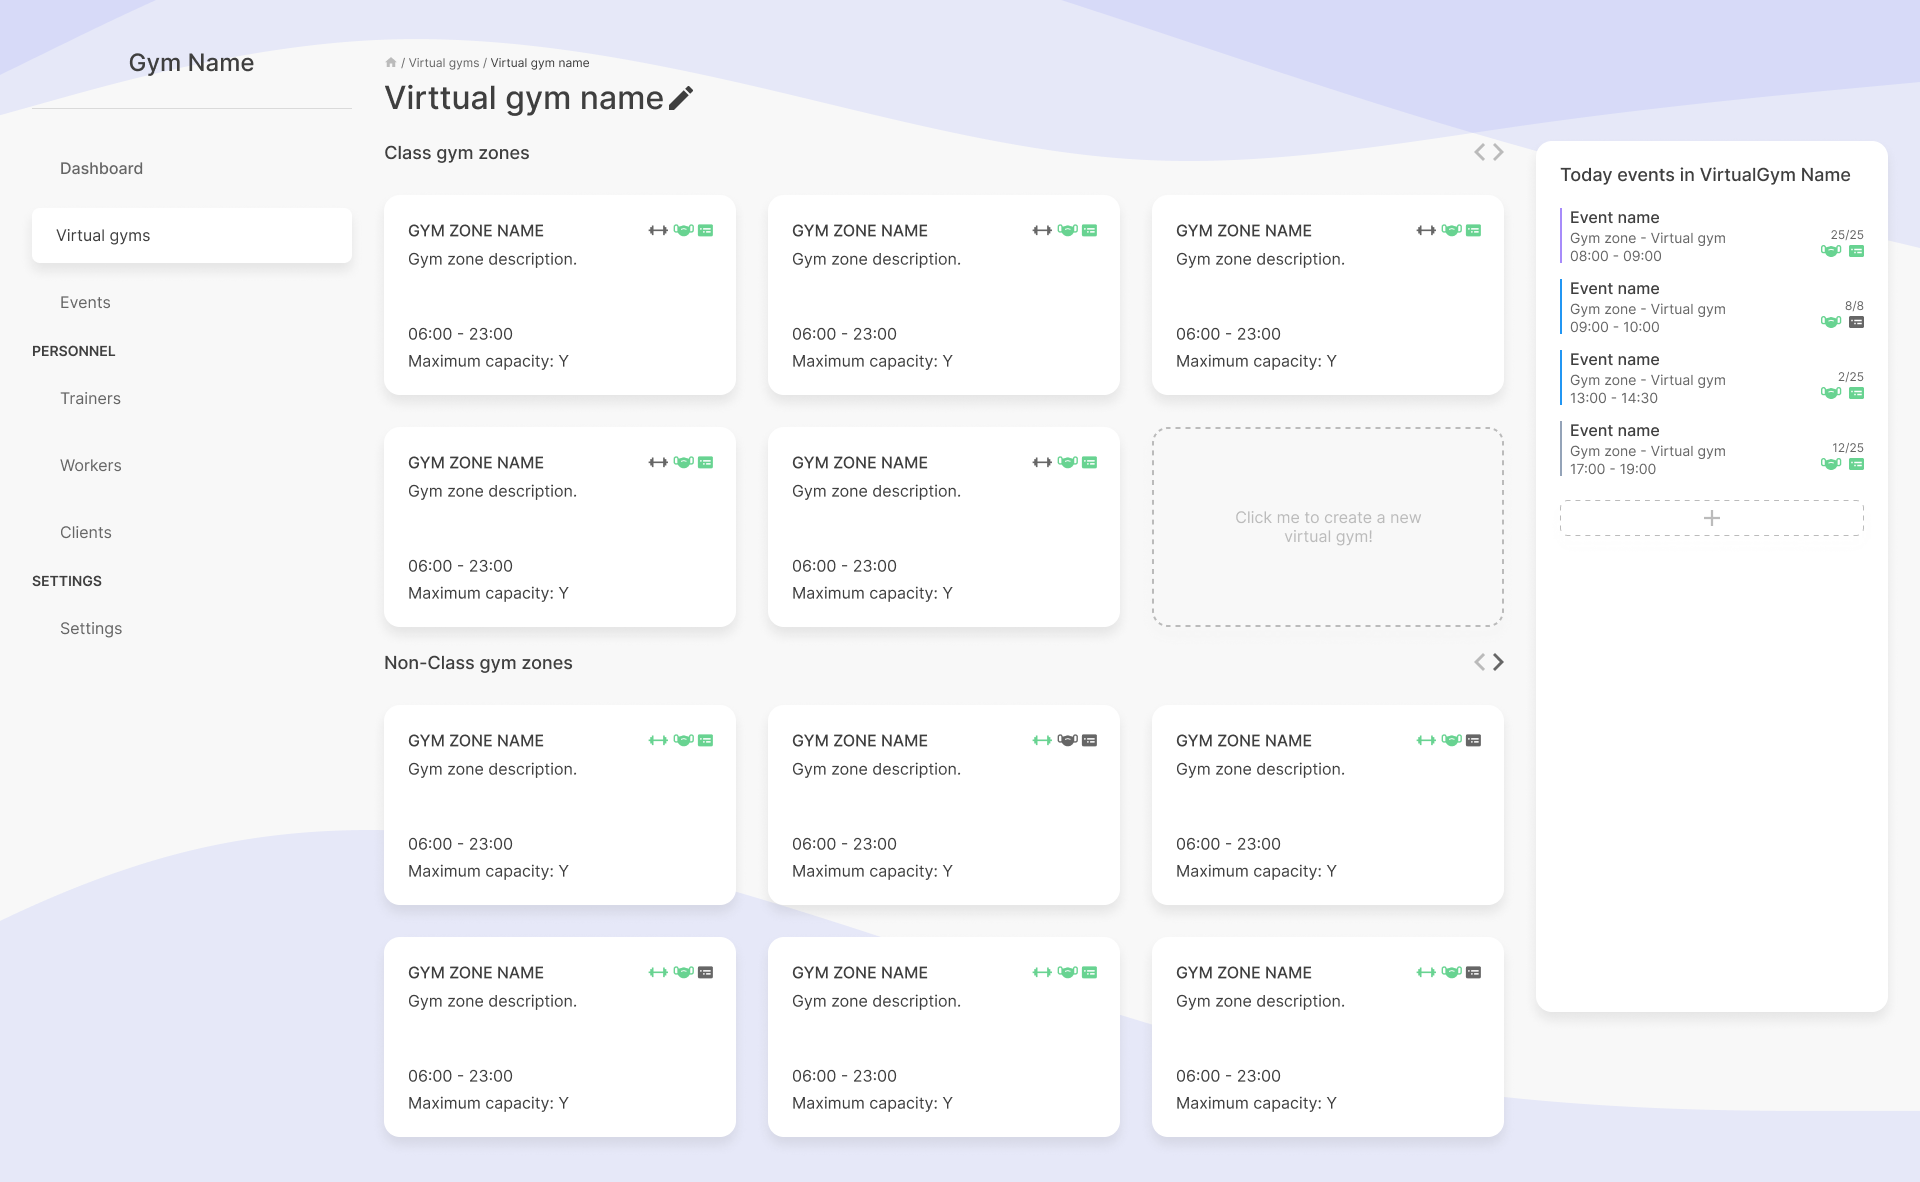
\includegraphics[width=\textwidth]{assets/ui/VirtualGym.png}
	\caption{Single virtual gym view, accessed by clicking on a virtual gym}
\end{figure}
\begin{figure}[H]
	\centering
	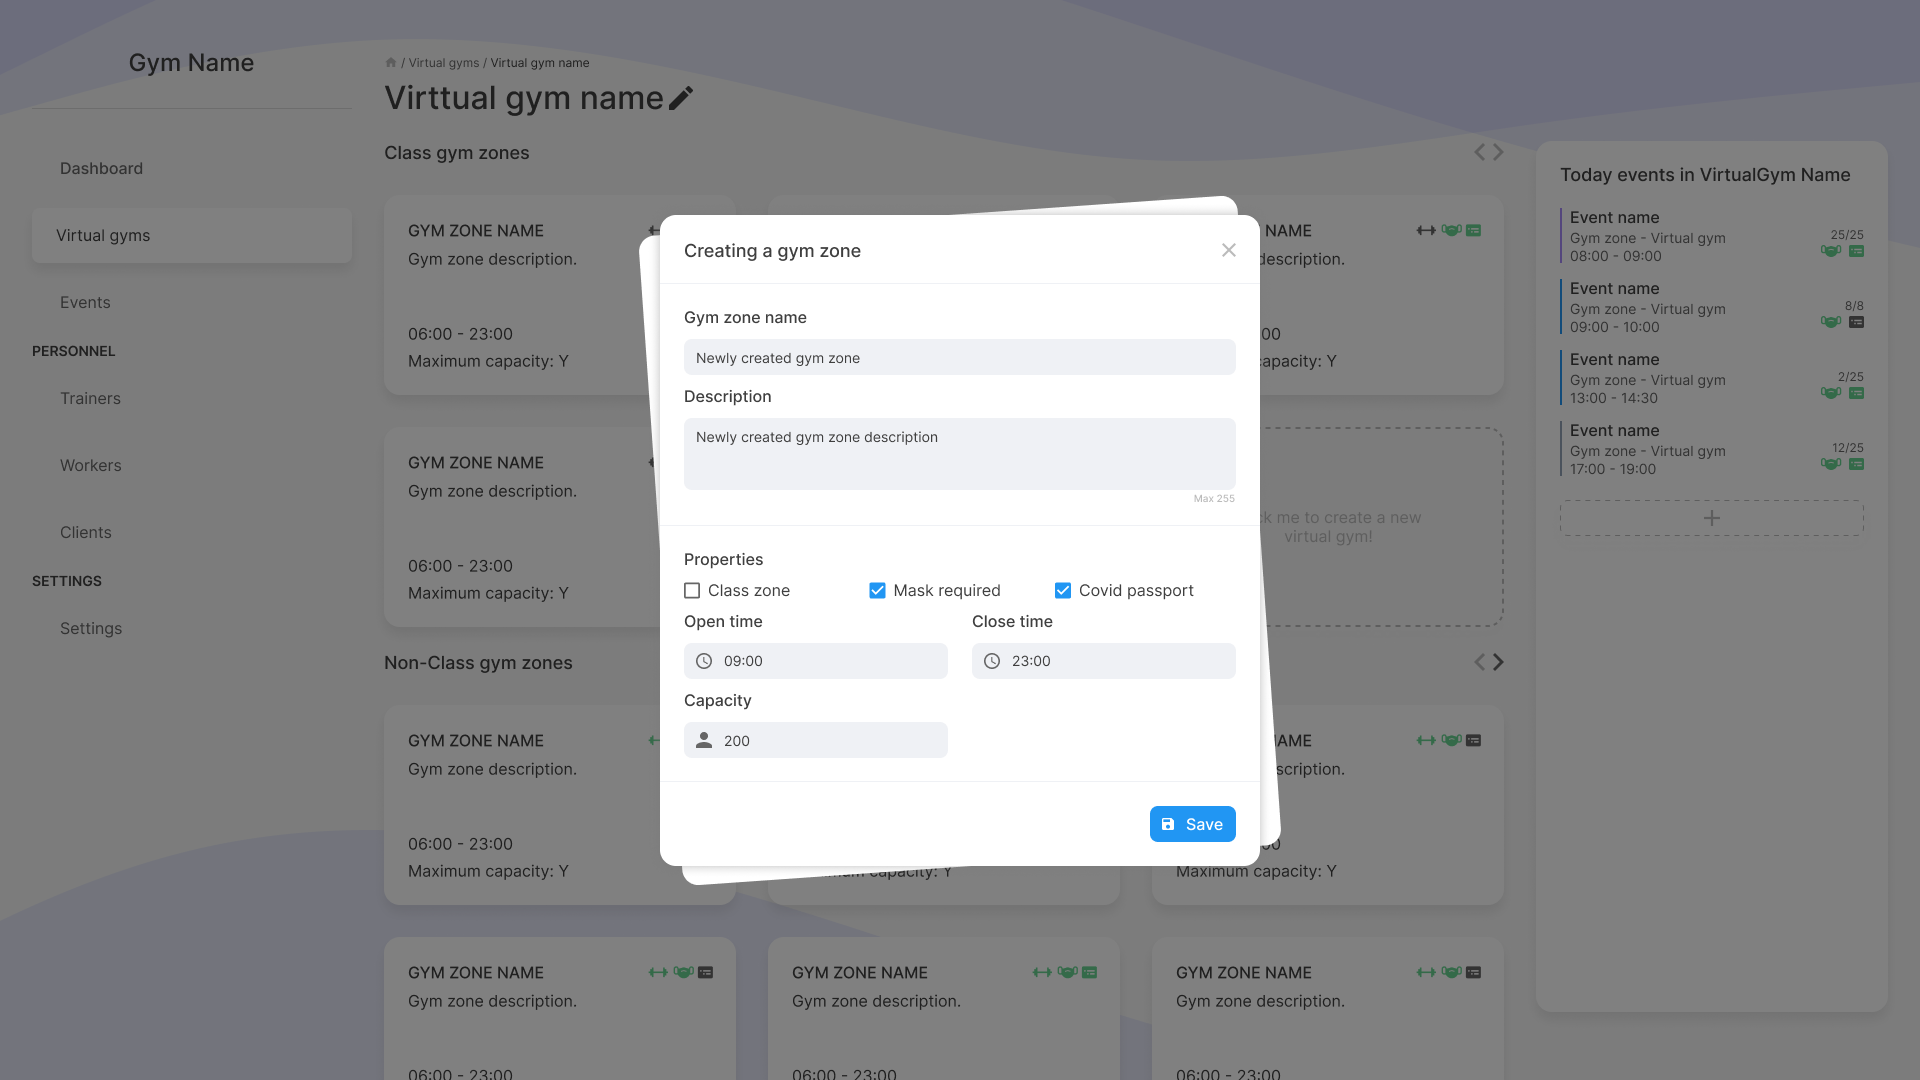
\includegraphics[width=\textwidth]{assets/ui/CreateGymZone.png}
	\caption{Gym zone dialog (create state)}
\end{figure}
\begin{figure}[H]
	\centering
	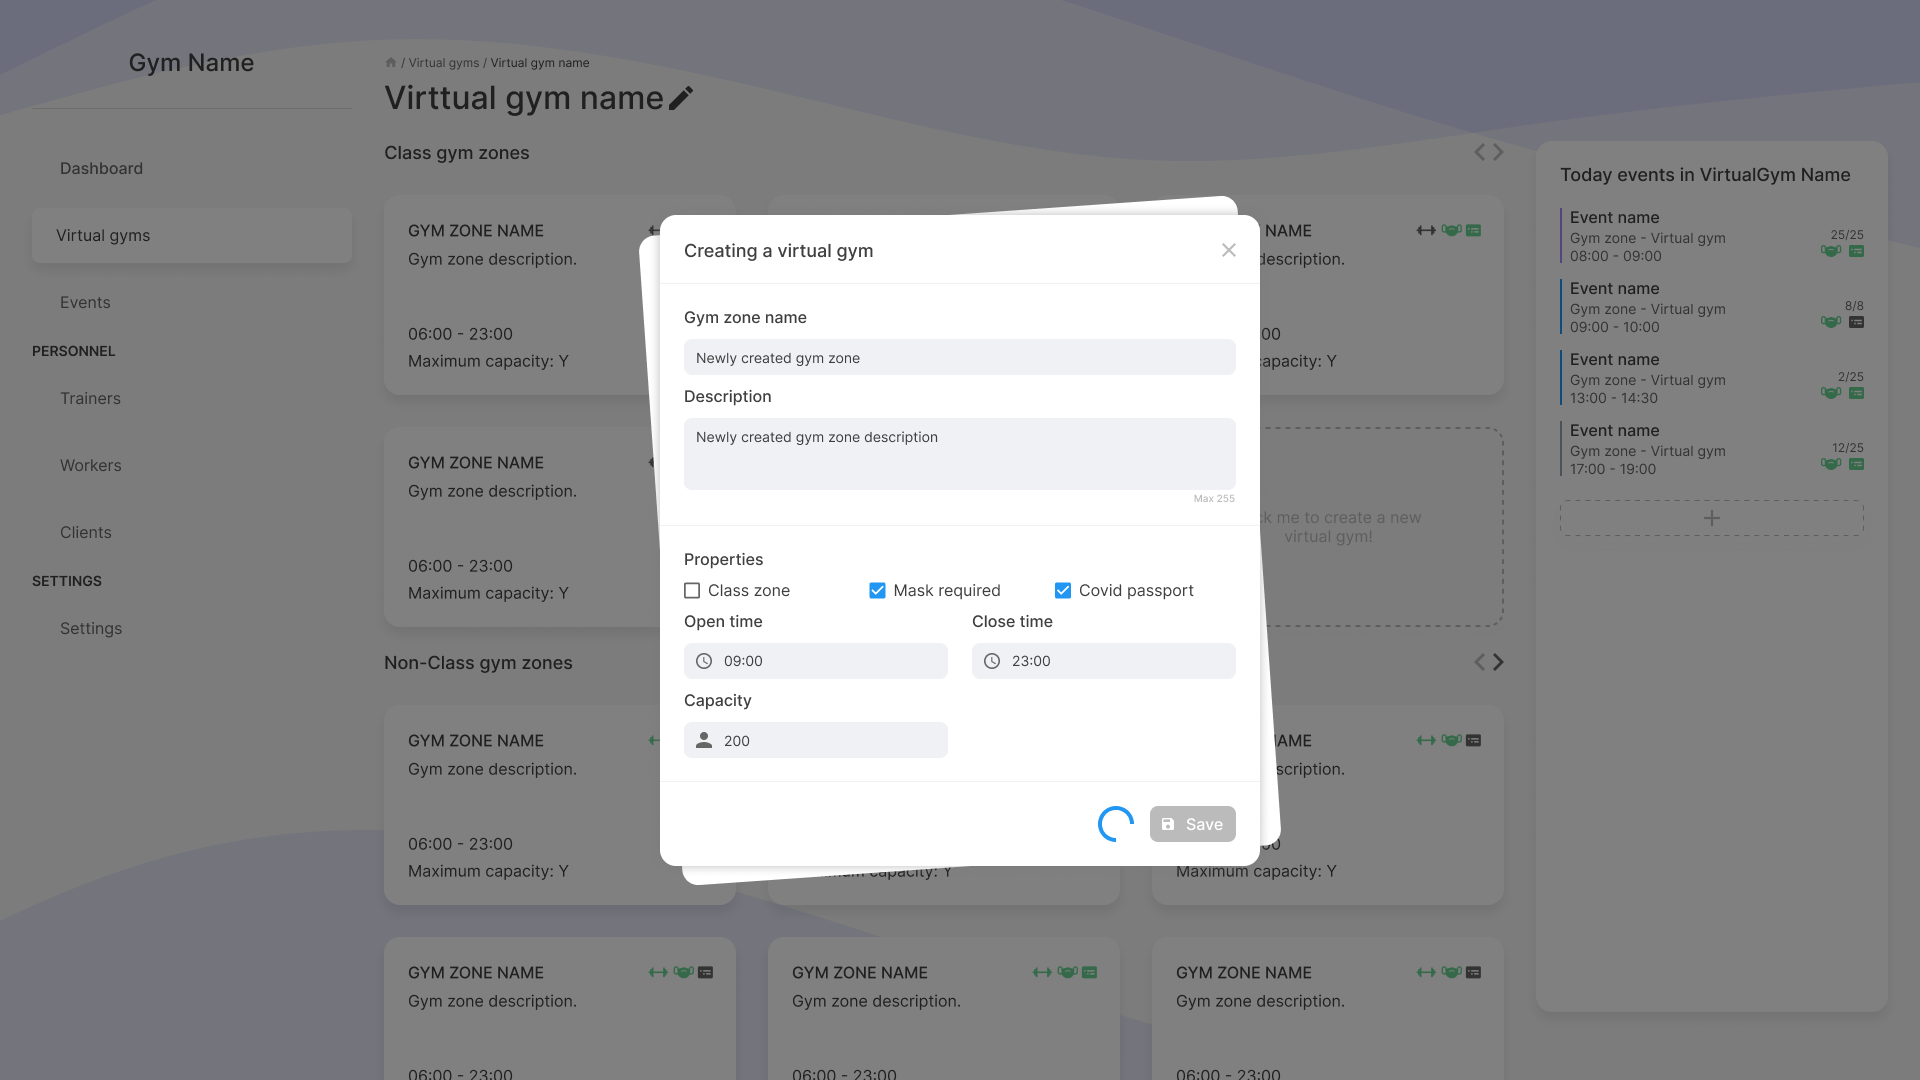
\includegraphics[width=\textwidth]{assets/ui/CreateLoadingGymZone.png}
	\caption{Gym zone dialog (create-loading state)}
\end{figure}
\begin{figure}[H]
	\centering
	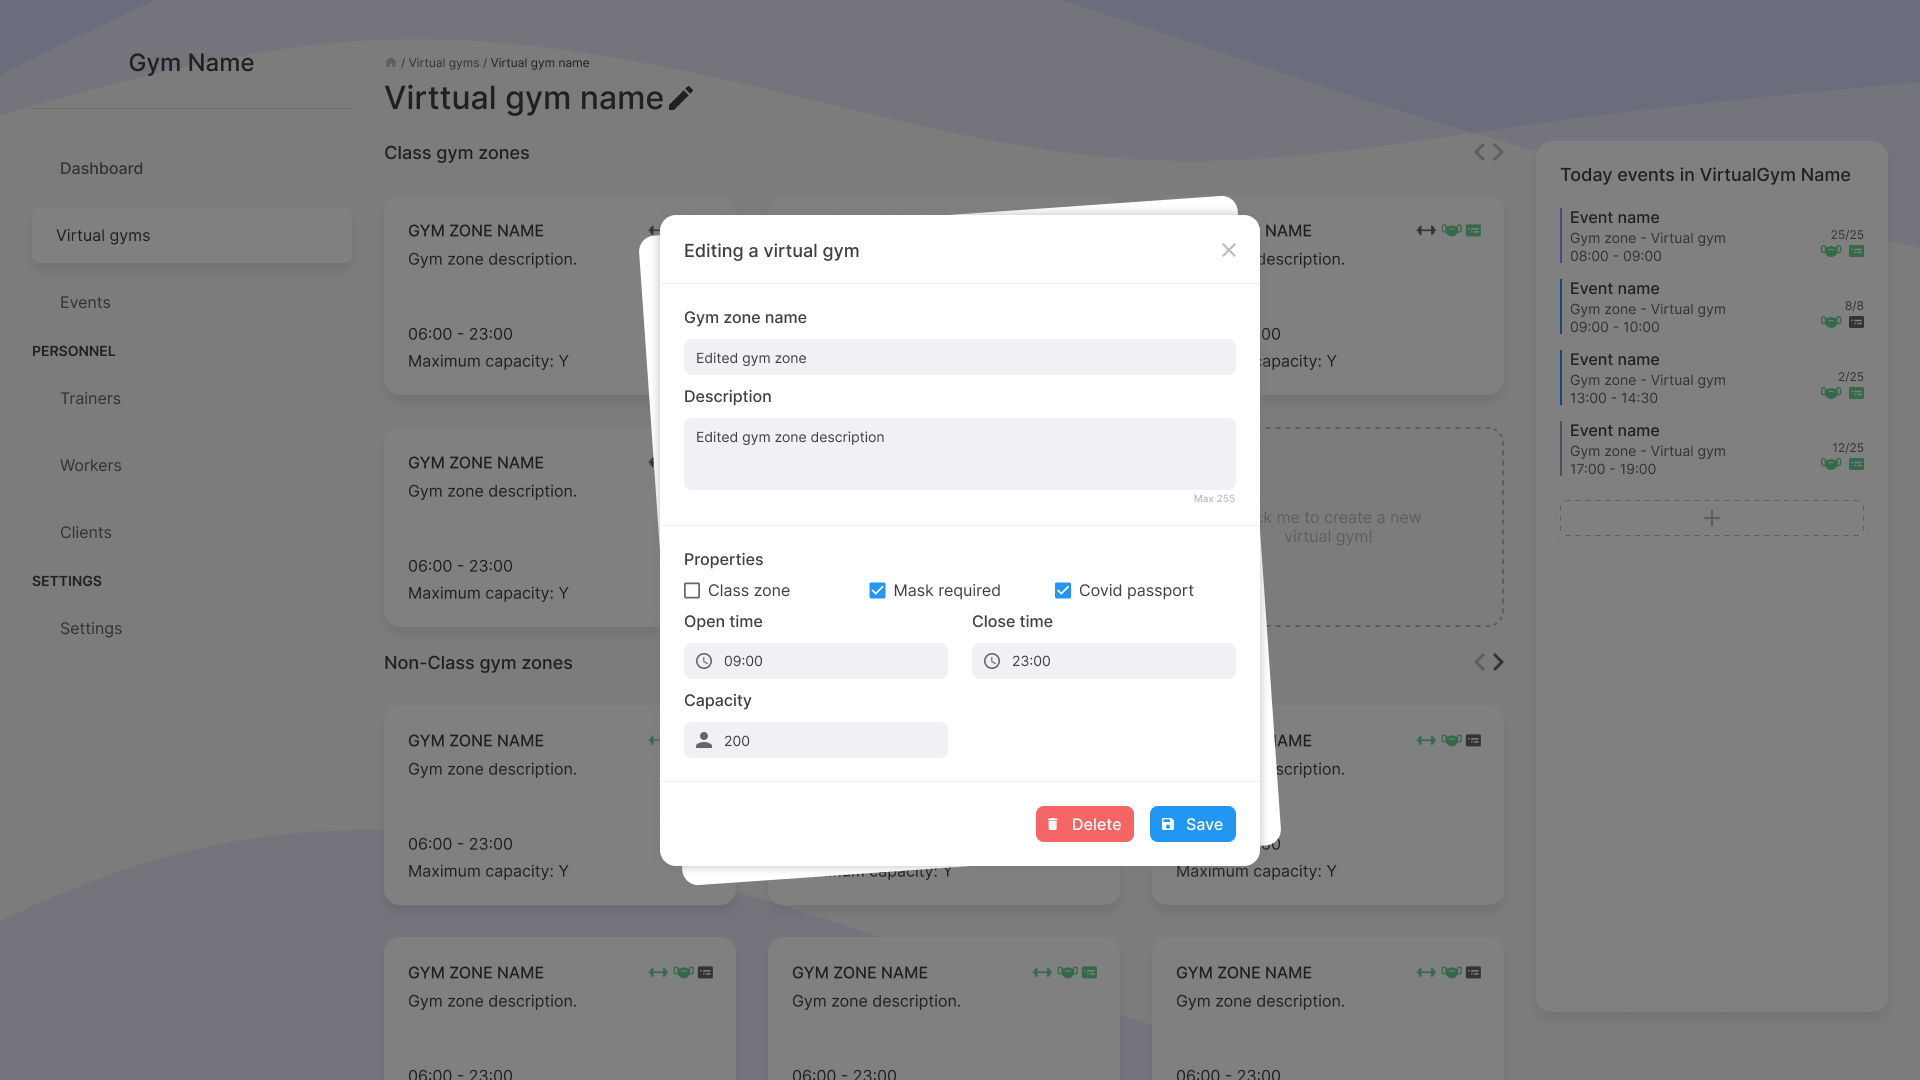
\includegraphics[width=\textwidth]{assets/ui/EditGymZone.png}
	\caption{Gym zone dialog (edit state)}
\end{figure}
\begin{figure}[H]
	\centering
	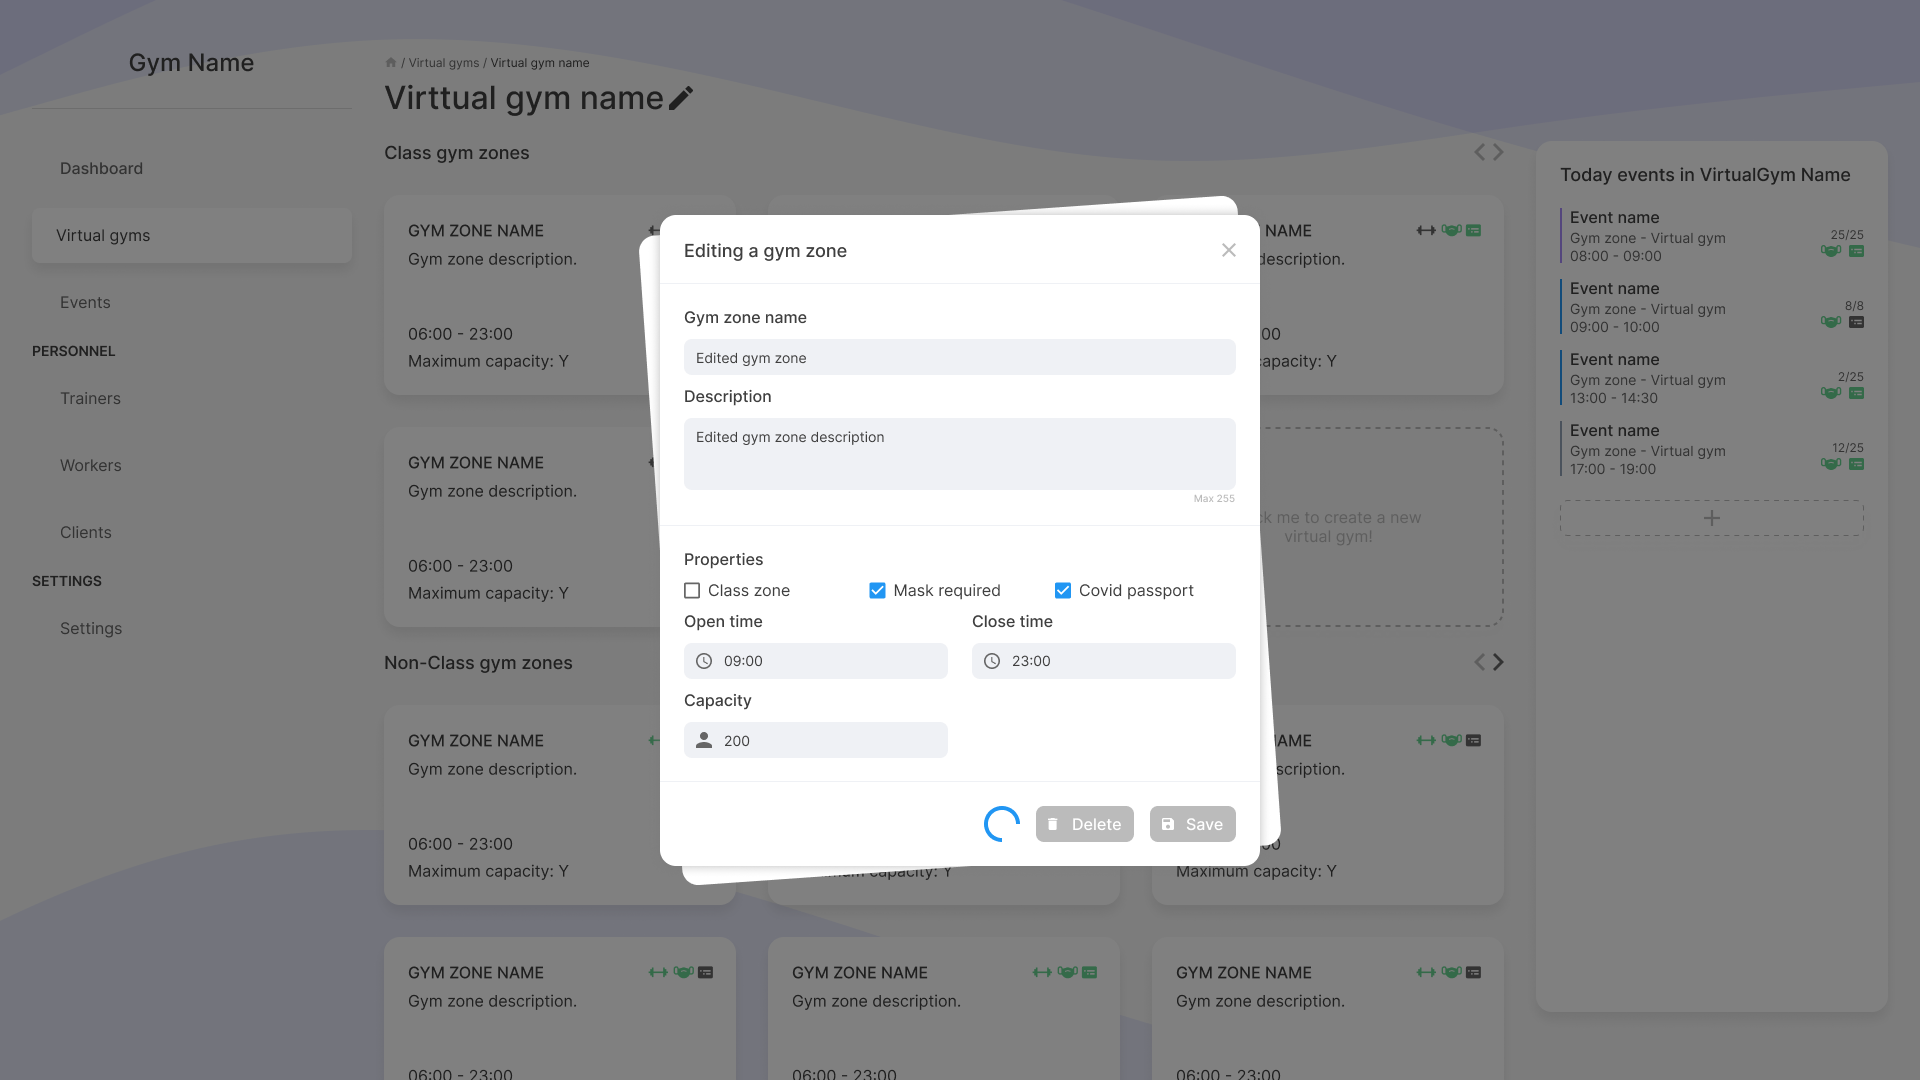
\includegraphics[width=\textwidth]{assets/ui/EditLoadingGymZone.png}
	\caption{Gym zone dialog (edit-loading state)}
\end{figure}
\begin{figure}[H]
	\centering
	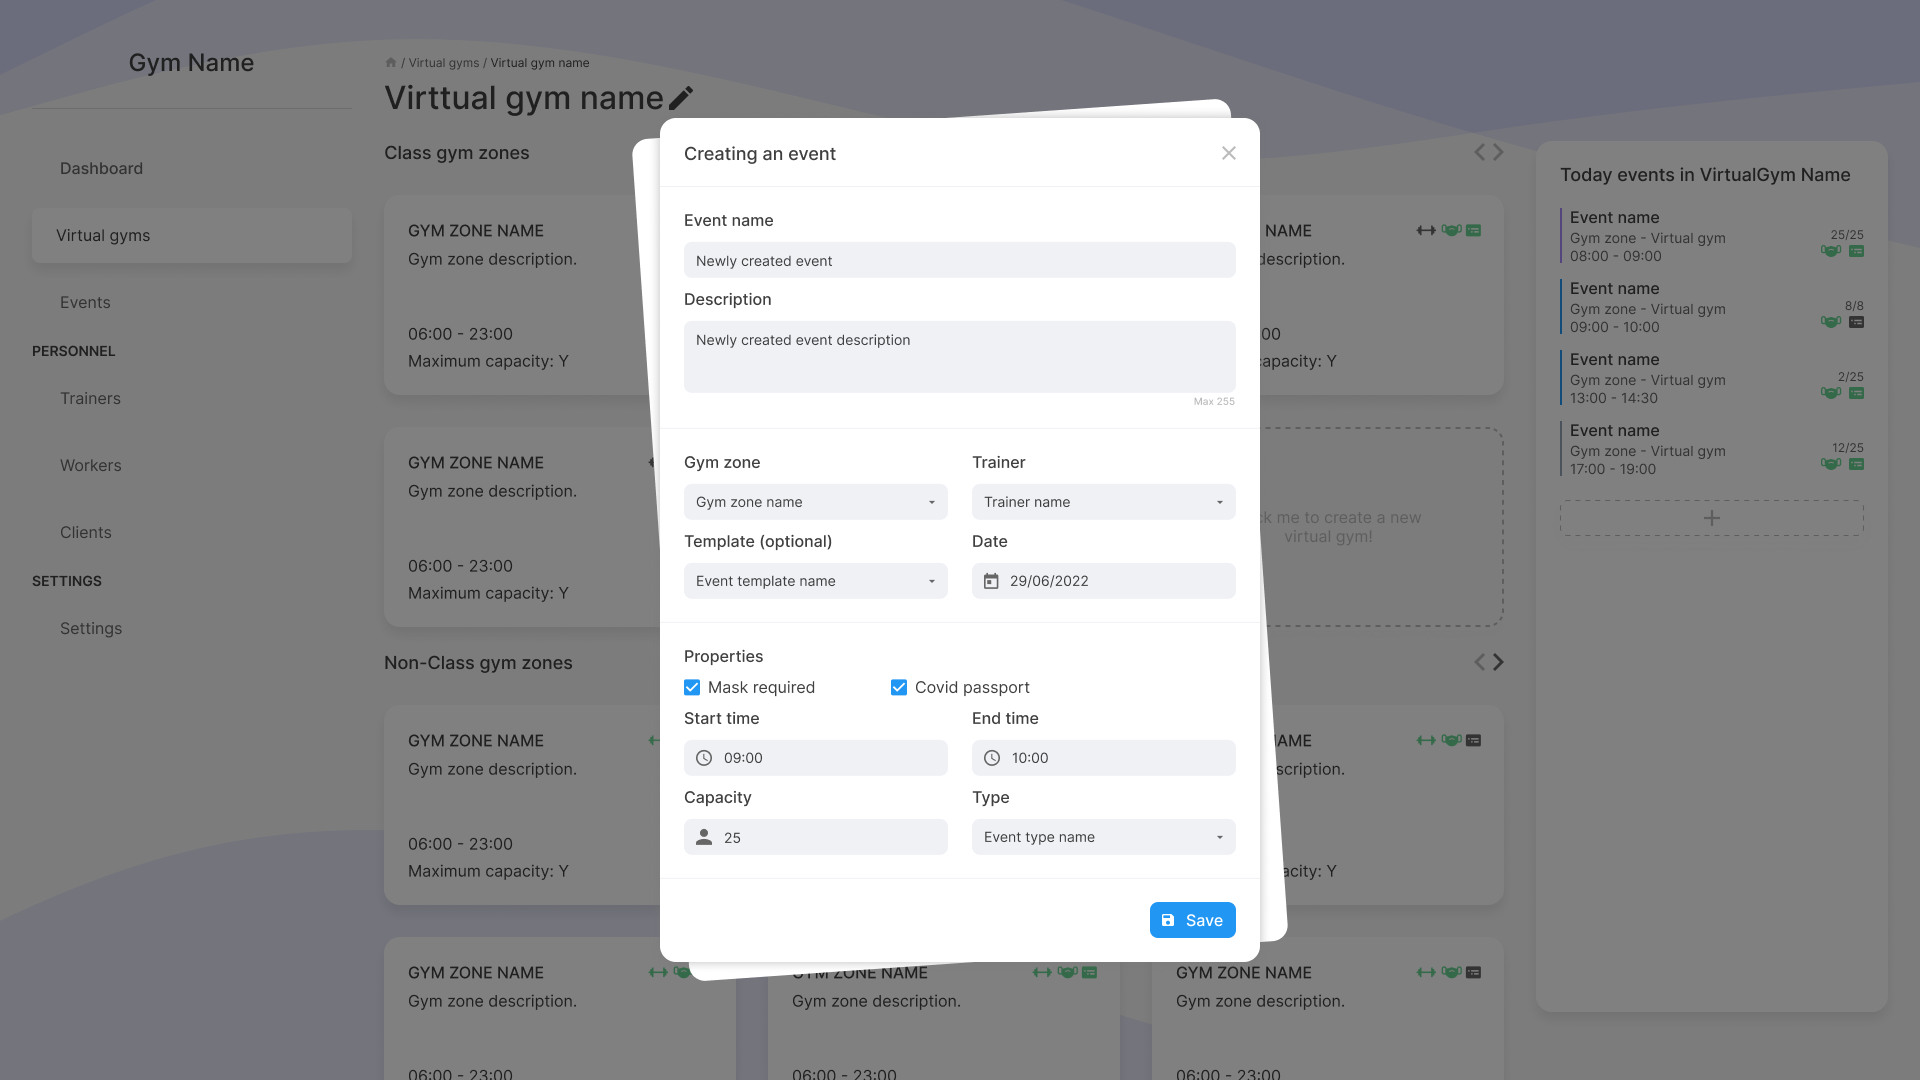
\includegraphics[width=\textwidth]{assets/ui/CreateEvent.png}
	\caption{Event dialog (create state)}
\end{figure}
\begin{figure}[H]
	\centering
	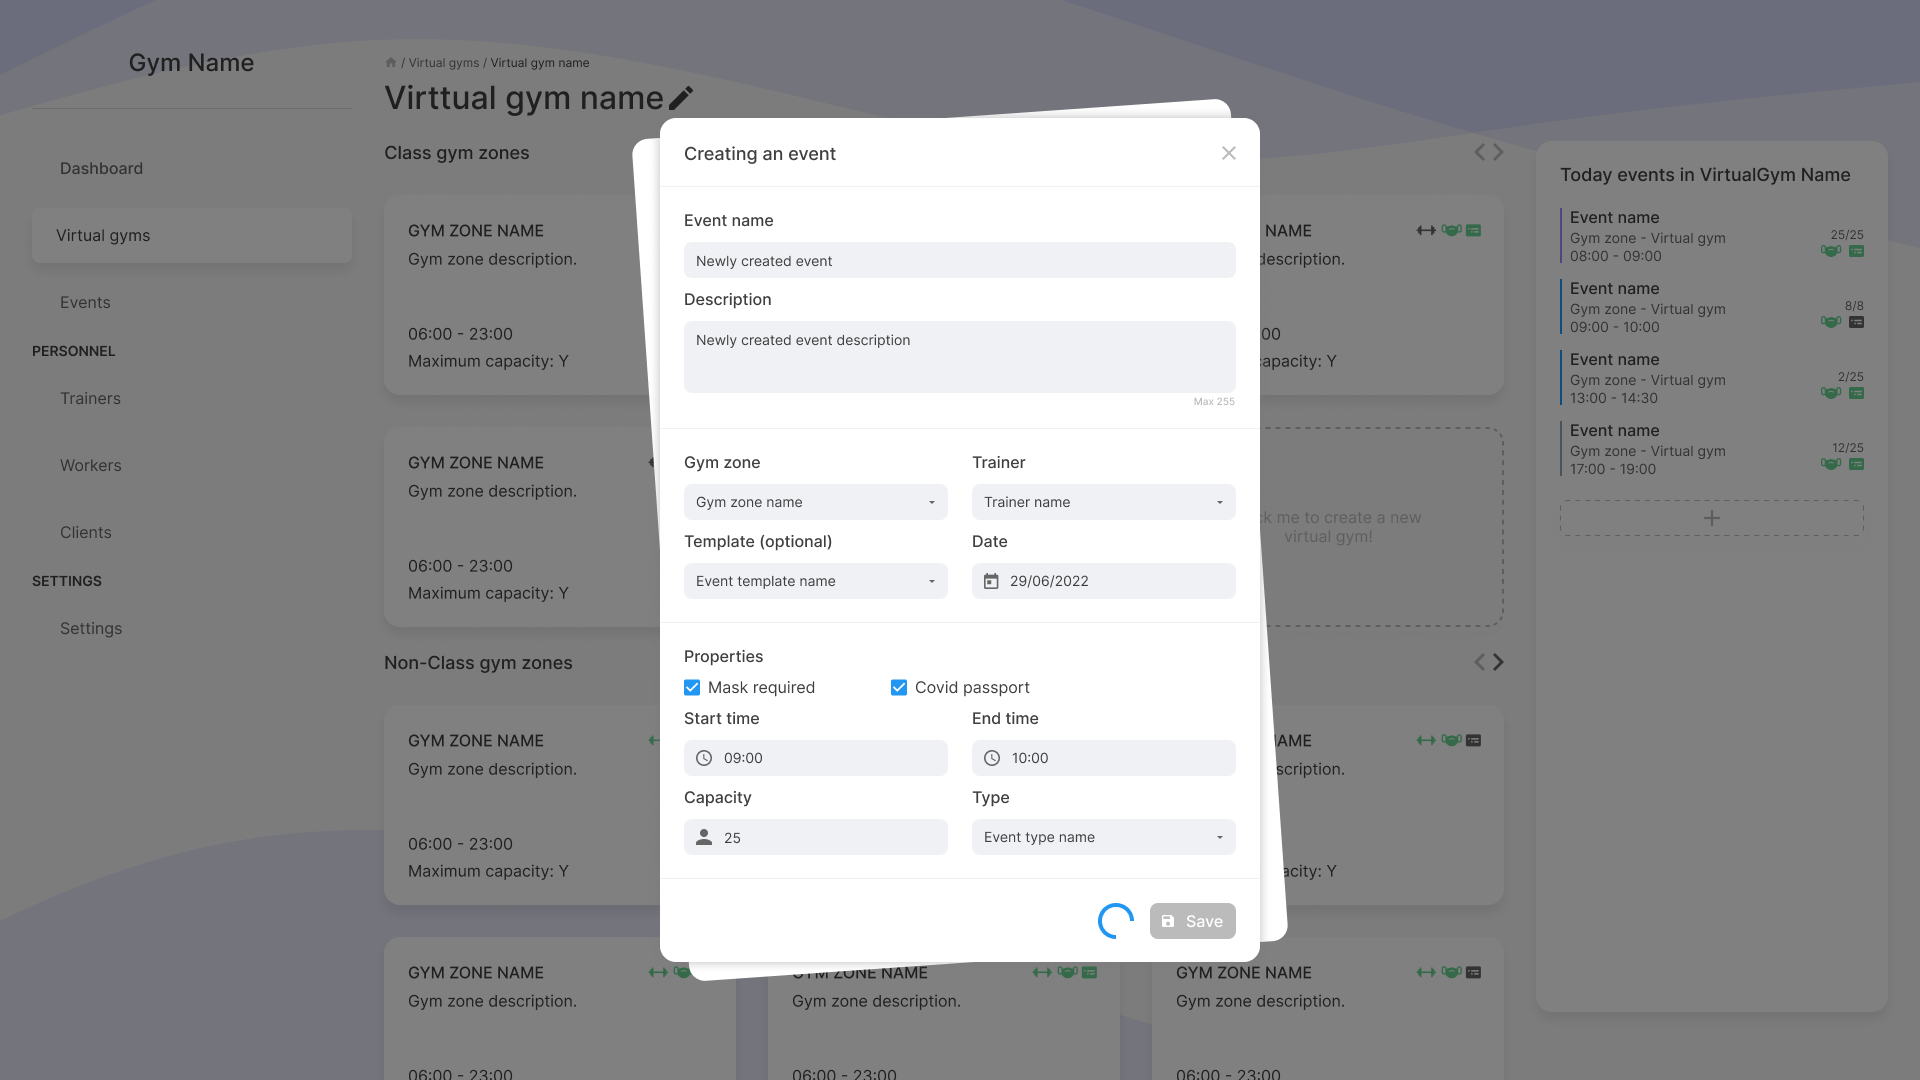
\includegraphics[width=\textwidth]{assets/ui/CreateLoadingEvent.png}
	\caption{Event dialog (create-loading state)}
\end{figure}
\begin{figure}[H]
	\centering
	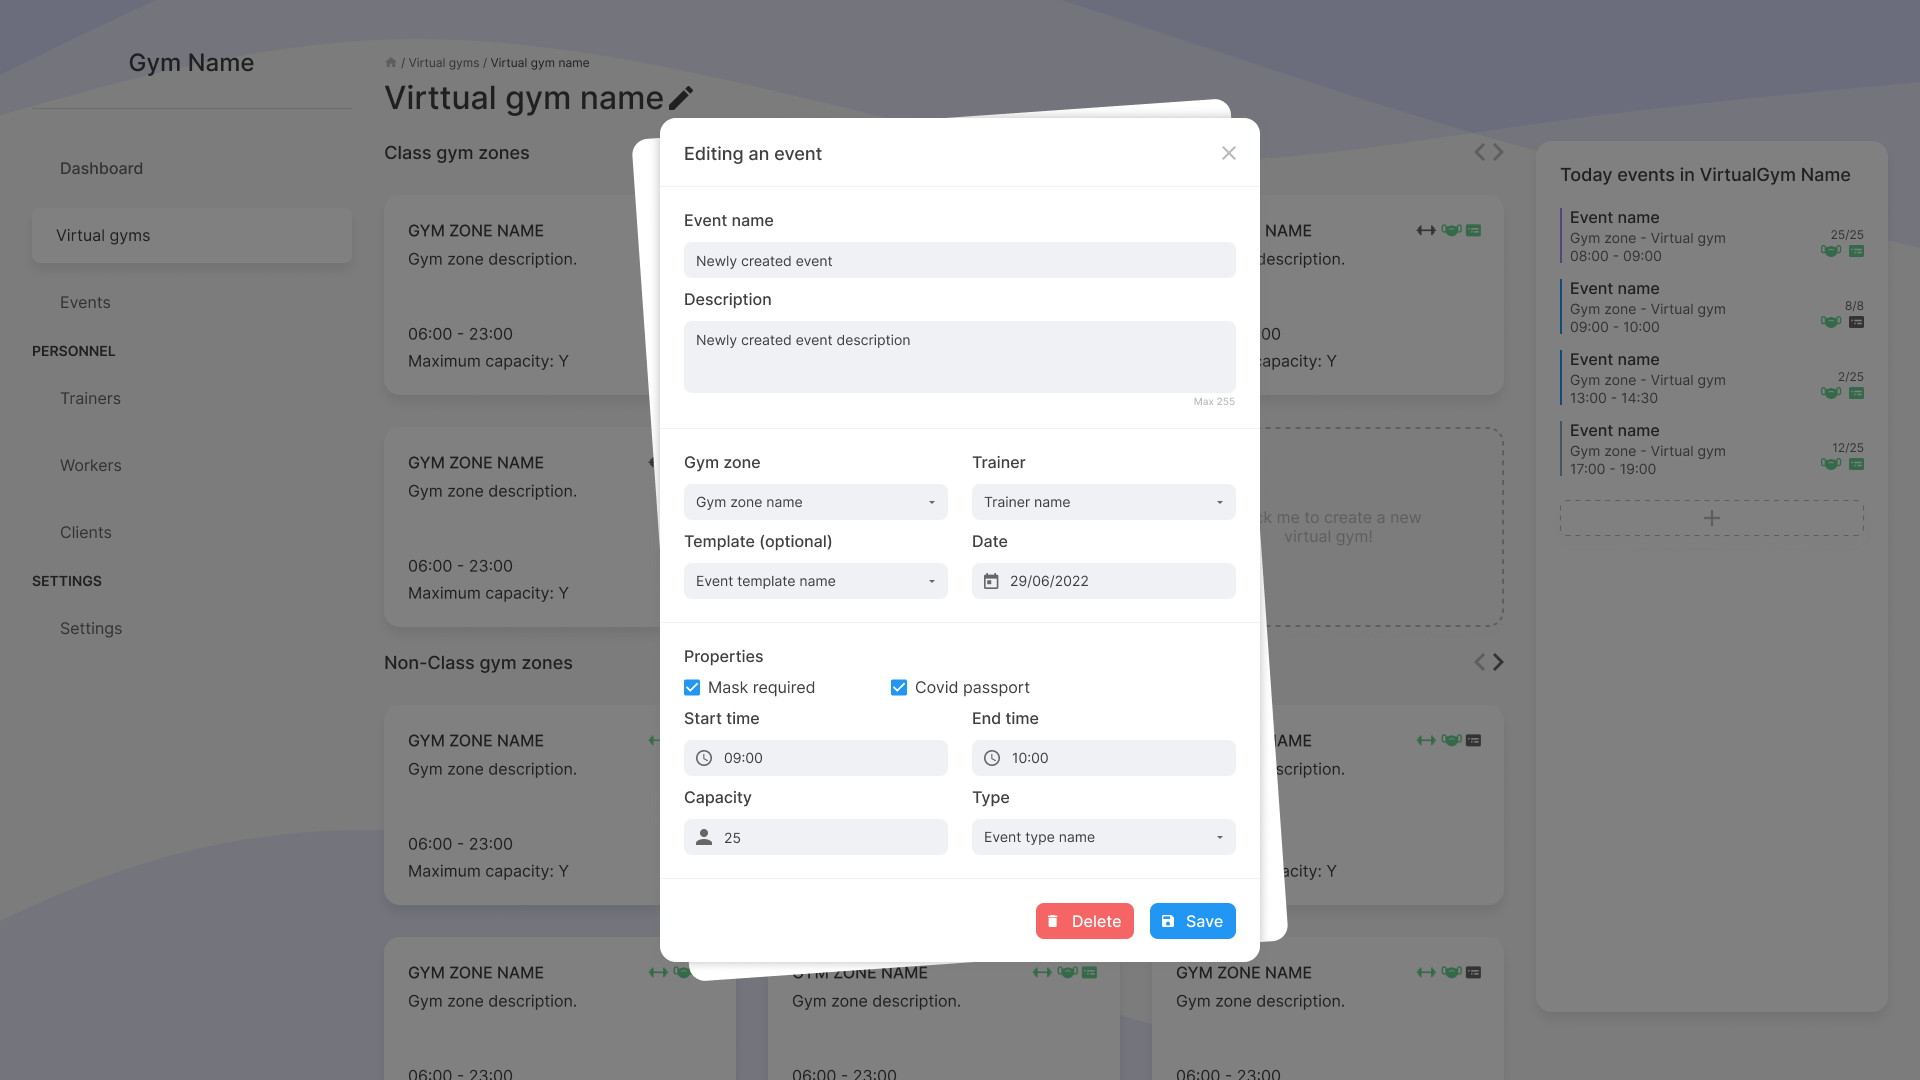
\includegraphics[width=\textwidth]{assets/ui/EditEvent.png}
	\caption{Event dialog (edit state)}
\end{figure}
\begin{figure}[H]
	\centering
	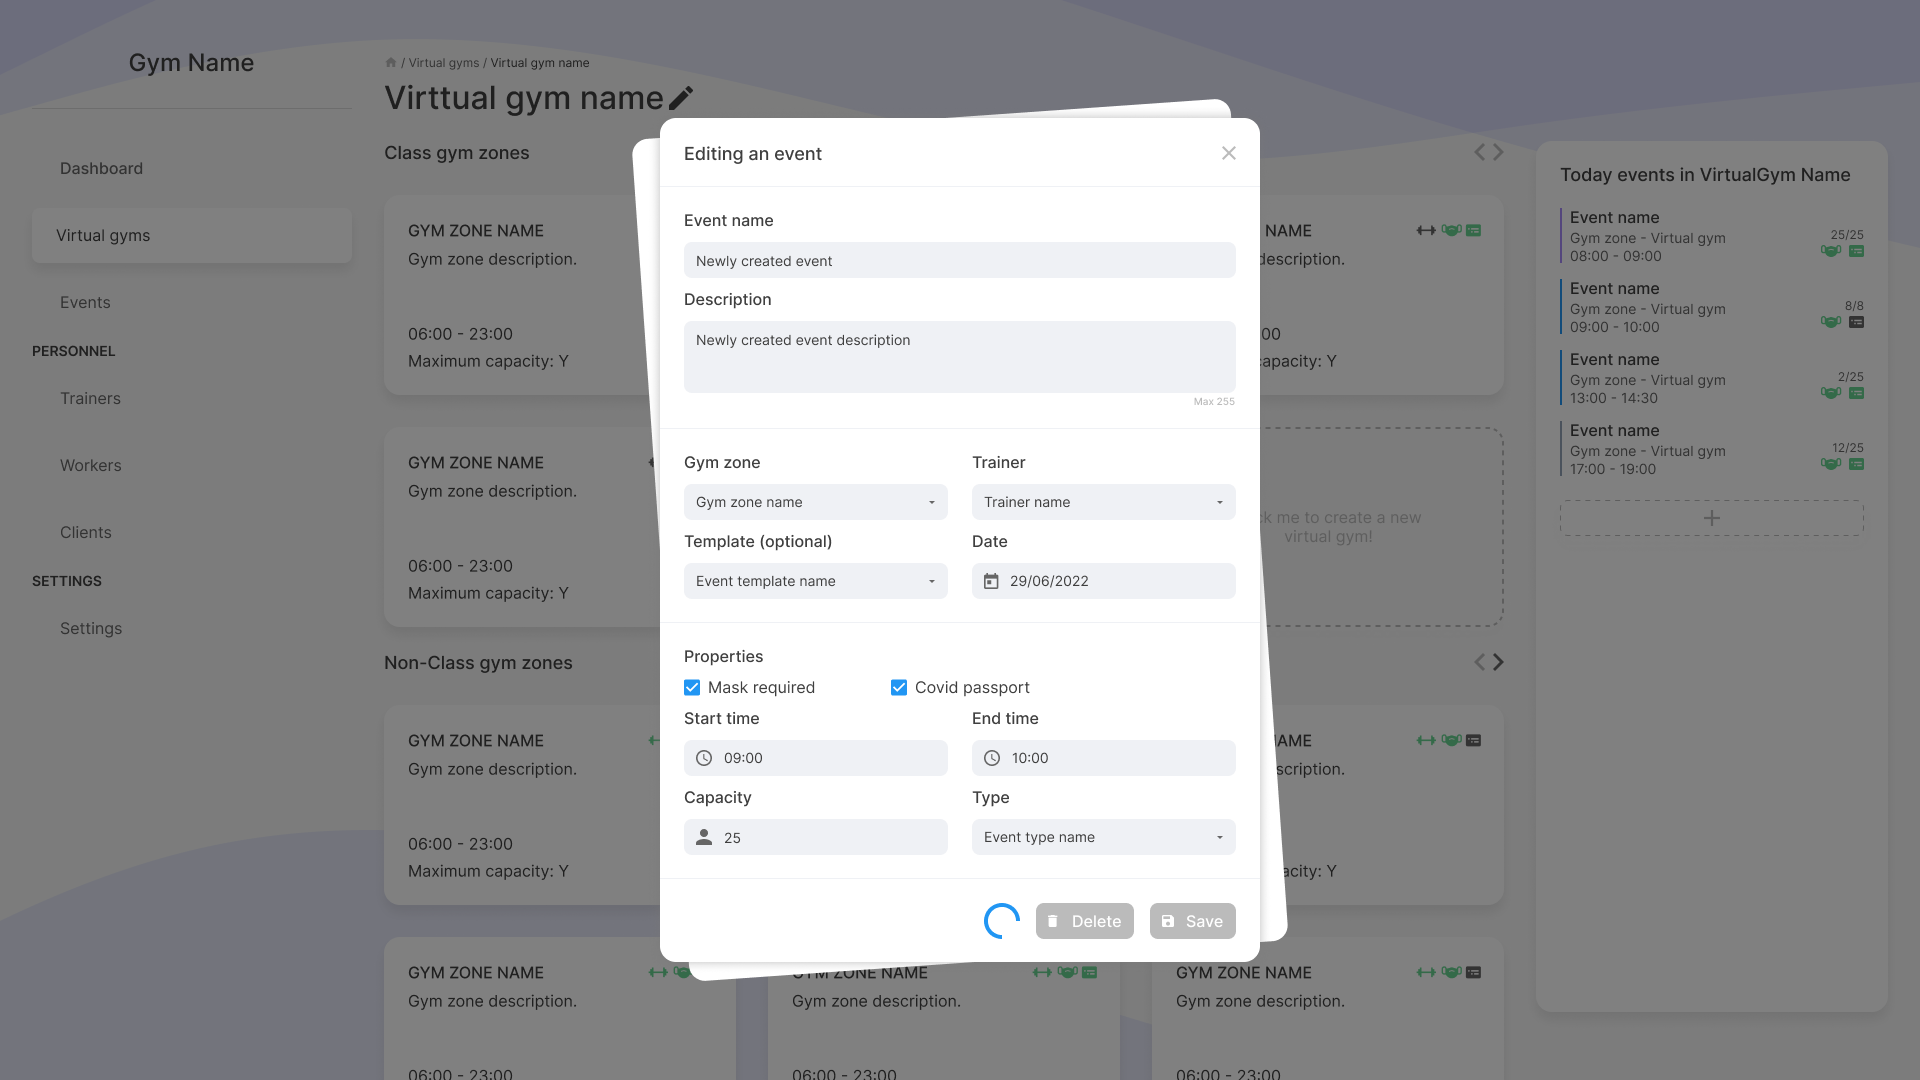
\includegraphics[width=\textwidth]{assets/ui/EditLoadingEvent.png}
	\caption{Event dialog (edit-loading state)}
\end{figure}
\begin{figure}[H]
	\centering
	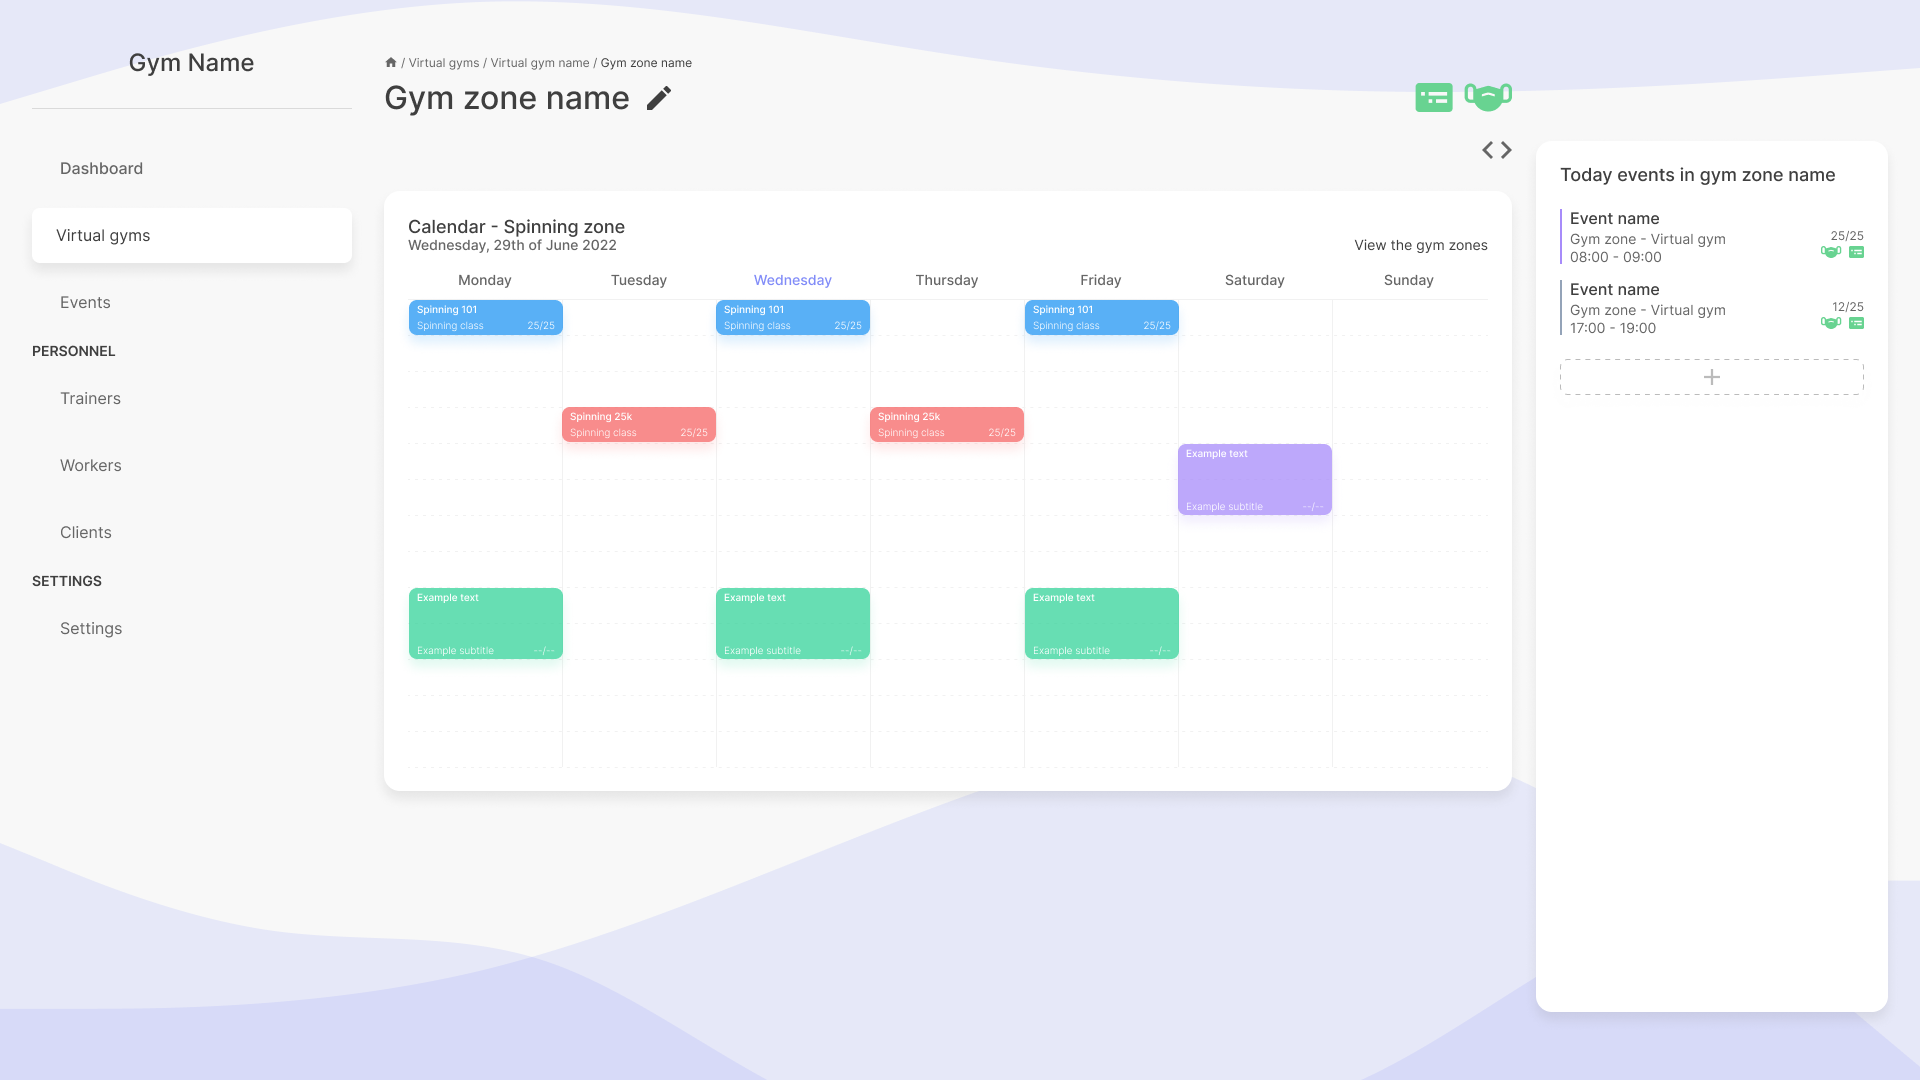
\includegraphics[width=\textwidth]{assets/ui/ClassGymZone.png}
	\caption{Class gym zone page, accessed by clicking on any class-type gym zone}
\end{figure}
\begin{figure}[H]
	\centering
	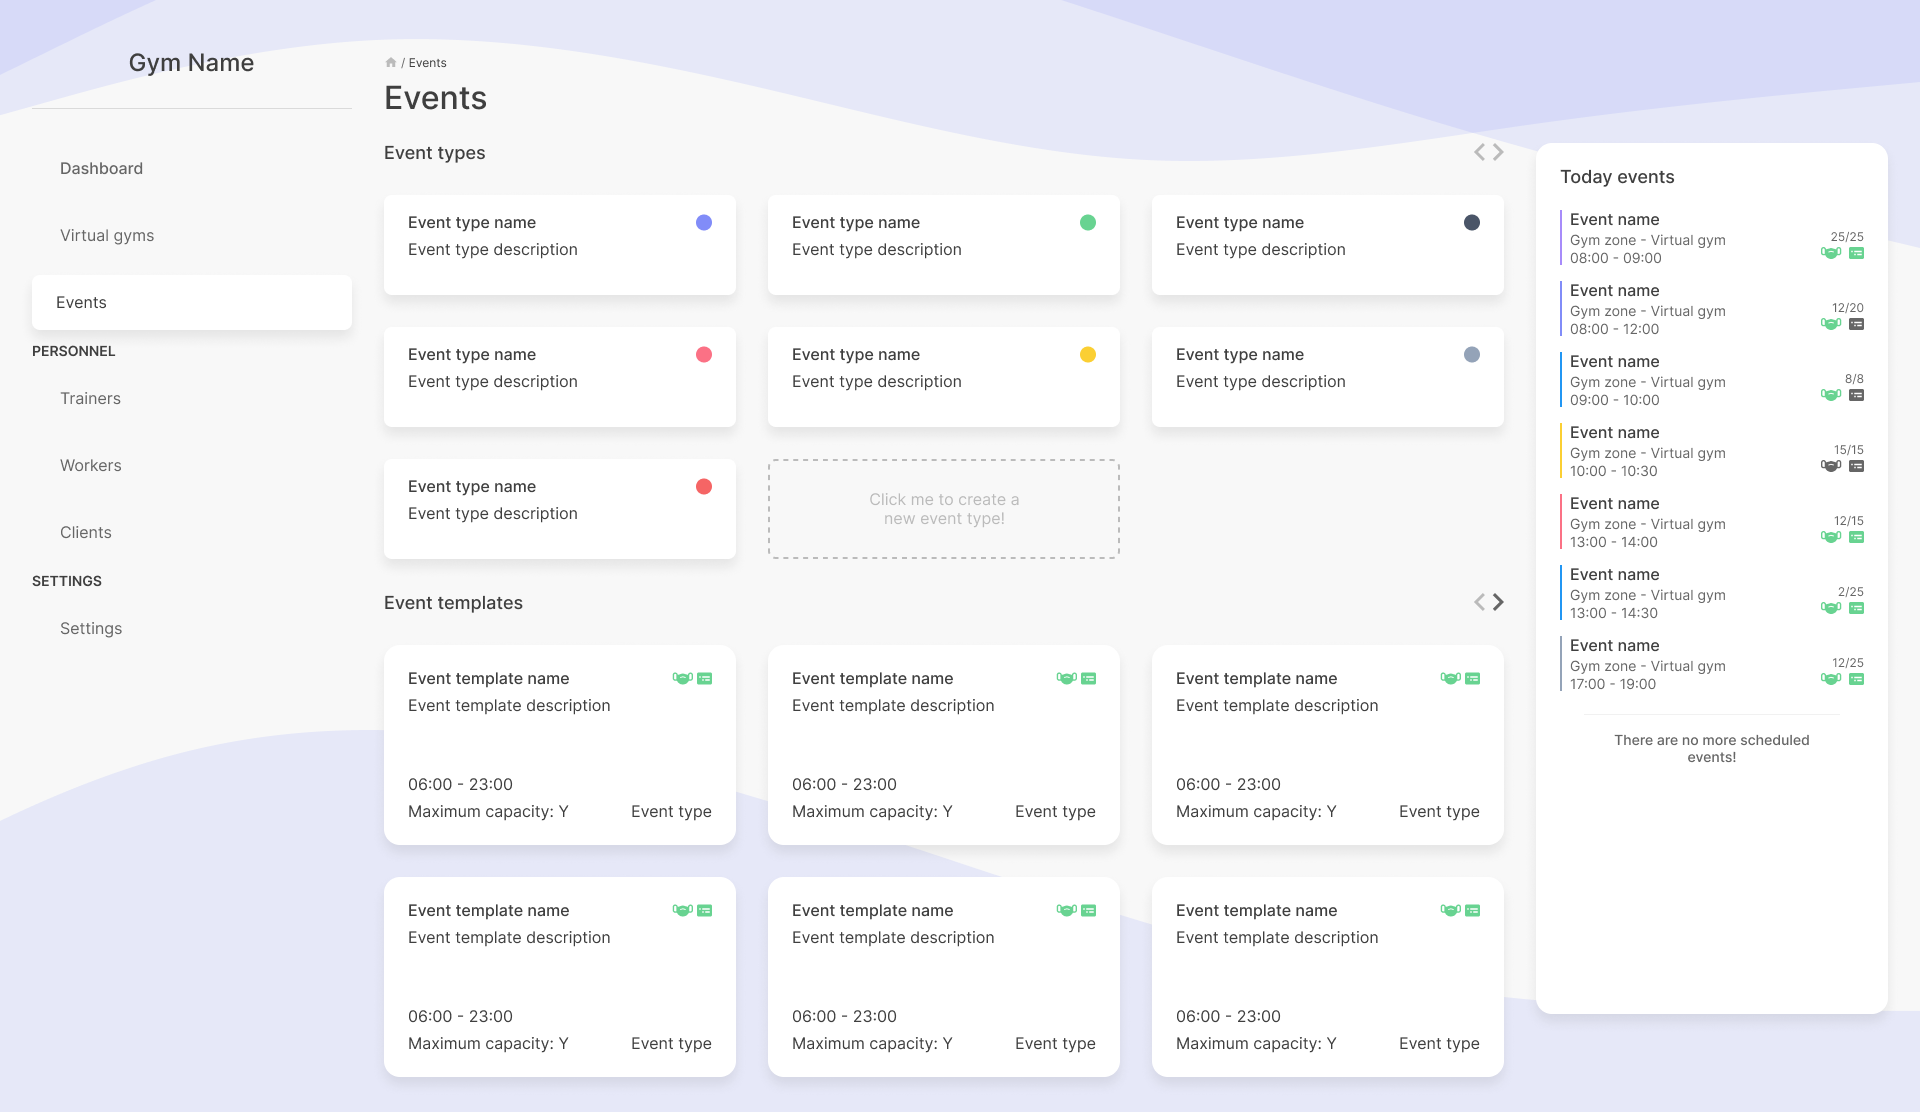
\includegraphics[width=\textwidth]{assets/ui/Events.png}
	\caption{Event's page, which is accessed using the left navigation bar}
\end{figure}
\begin{figure}[H]
	\centering
	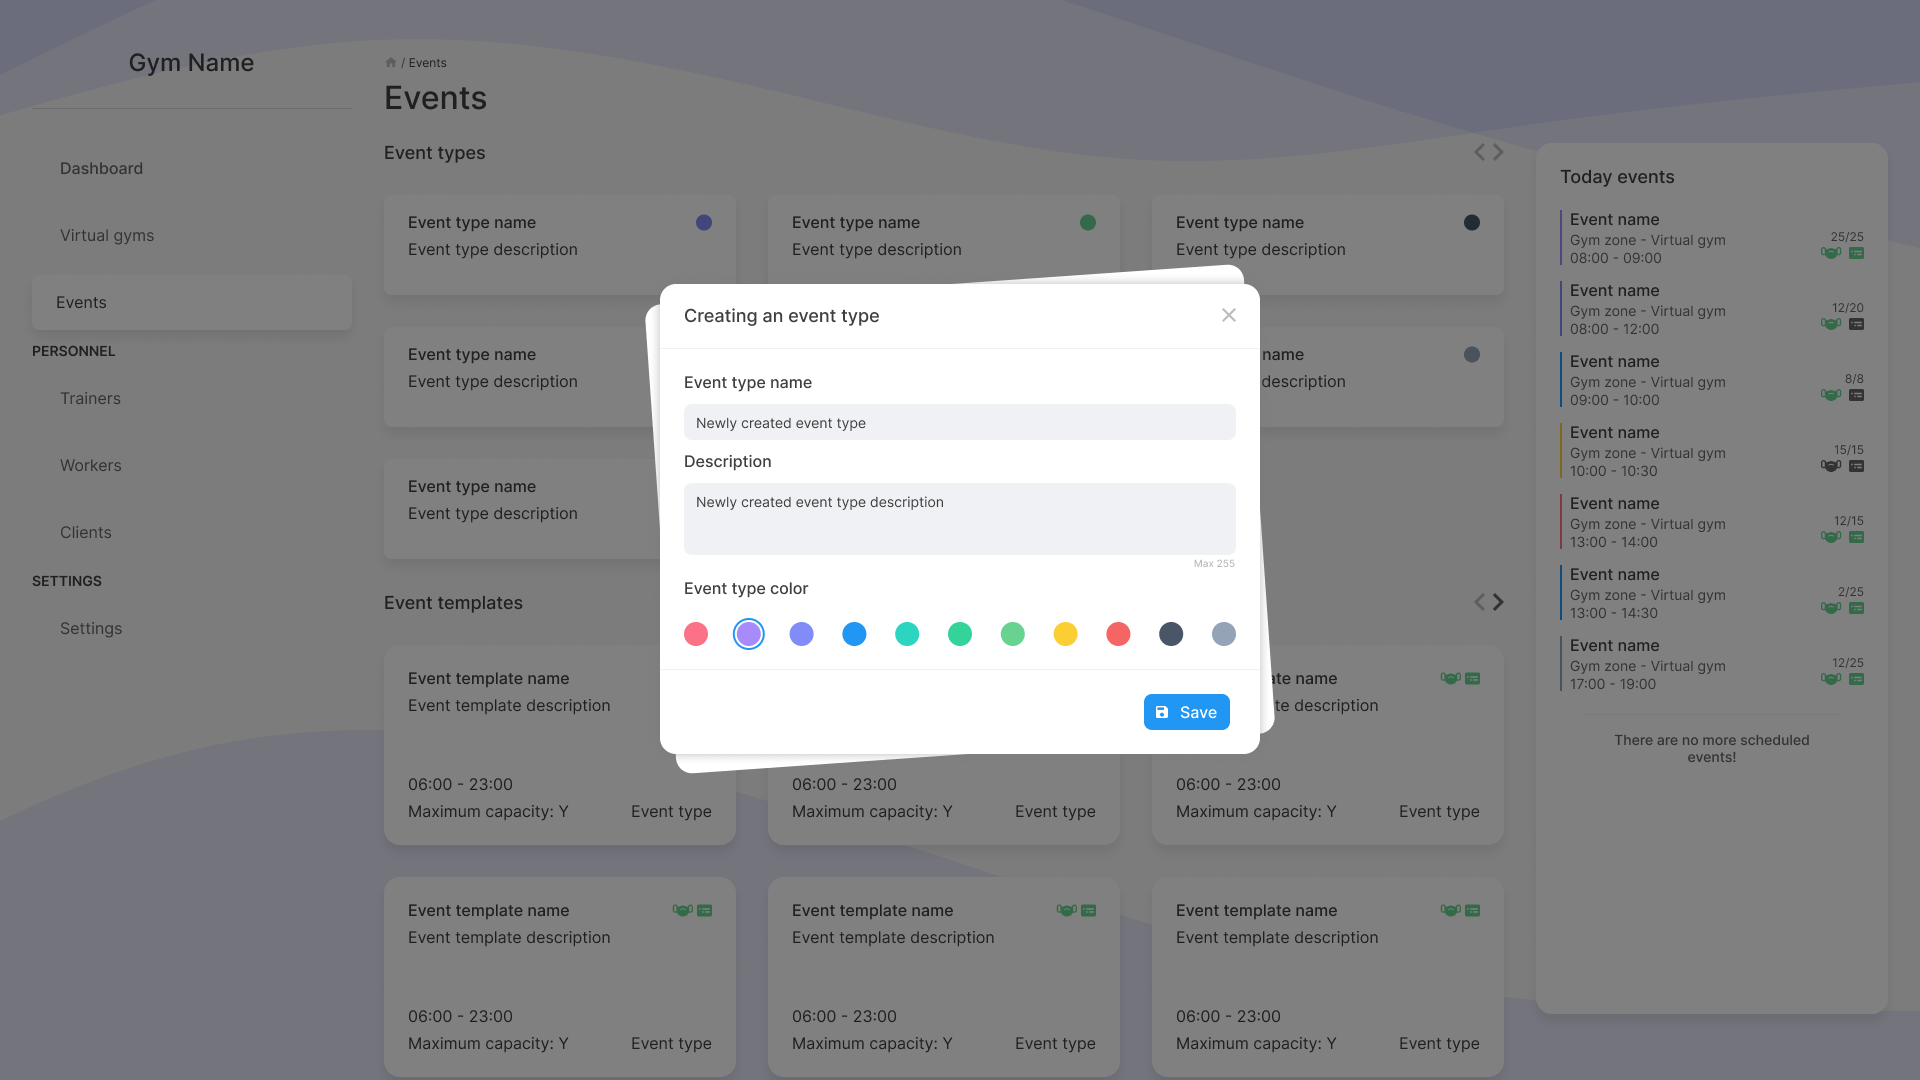
\includegraphics[width=\textwidth]{assets/ui/EventTypeCreate.png}
	\caption{Event type dialog (create state)}
\end{figure}
\begin{figure}[H]
	\centering
	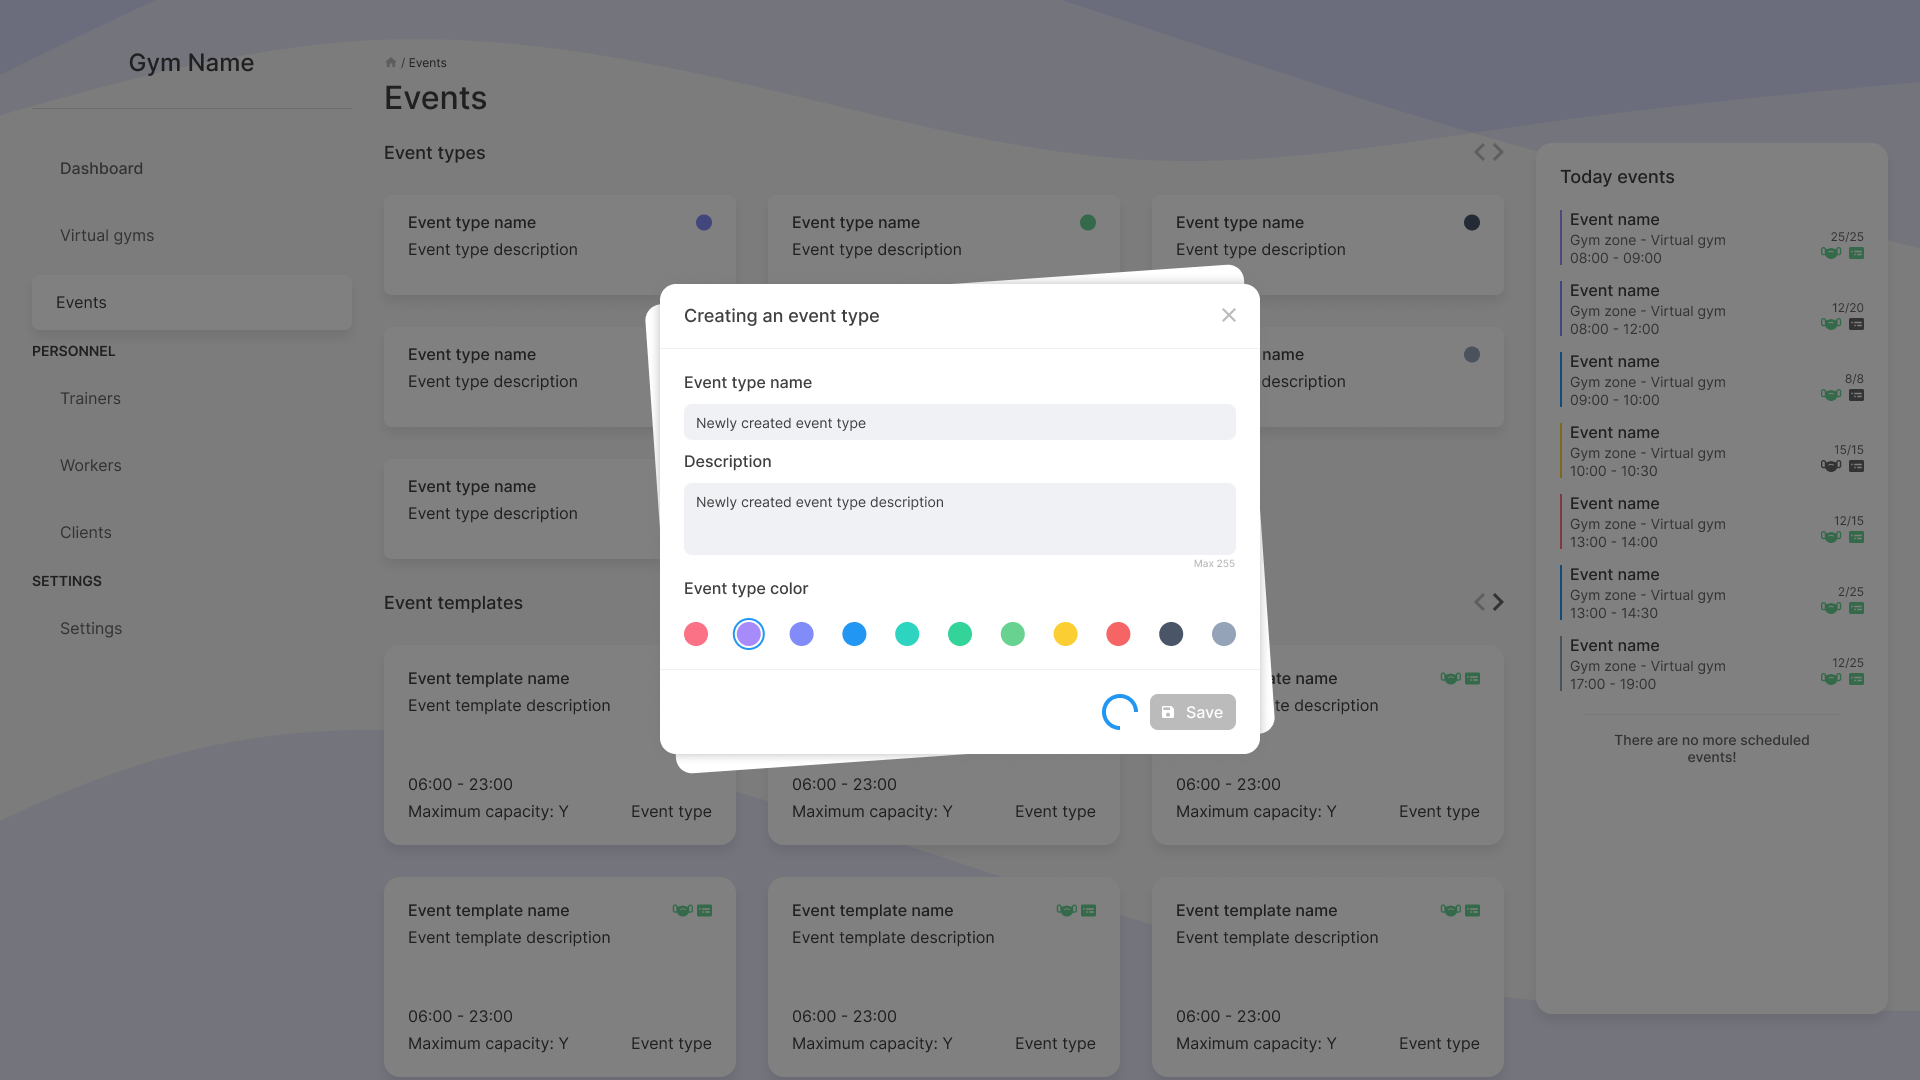
\includegraphics[width=\textwidth]{assets/ui/EventTypeCreateLoading.png}
	\caption{Event type dialog (create-loading state)}
\end{figure}
\begin{figure}[H]
	\centering
	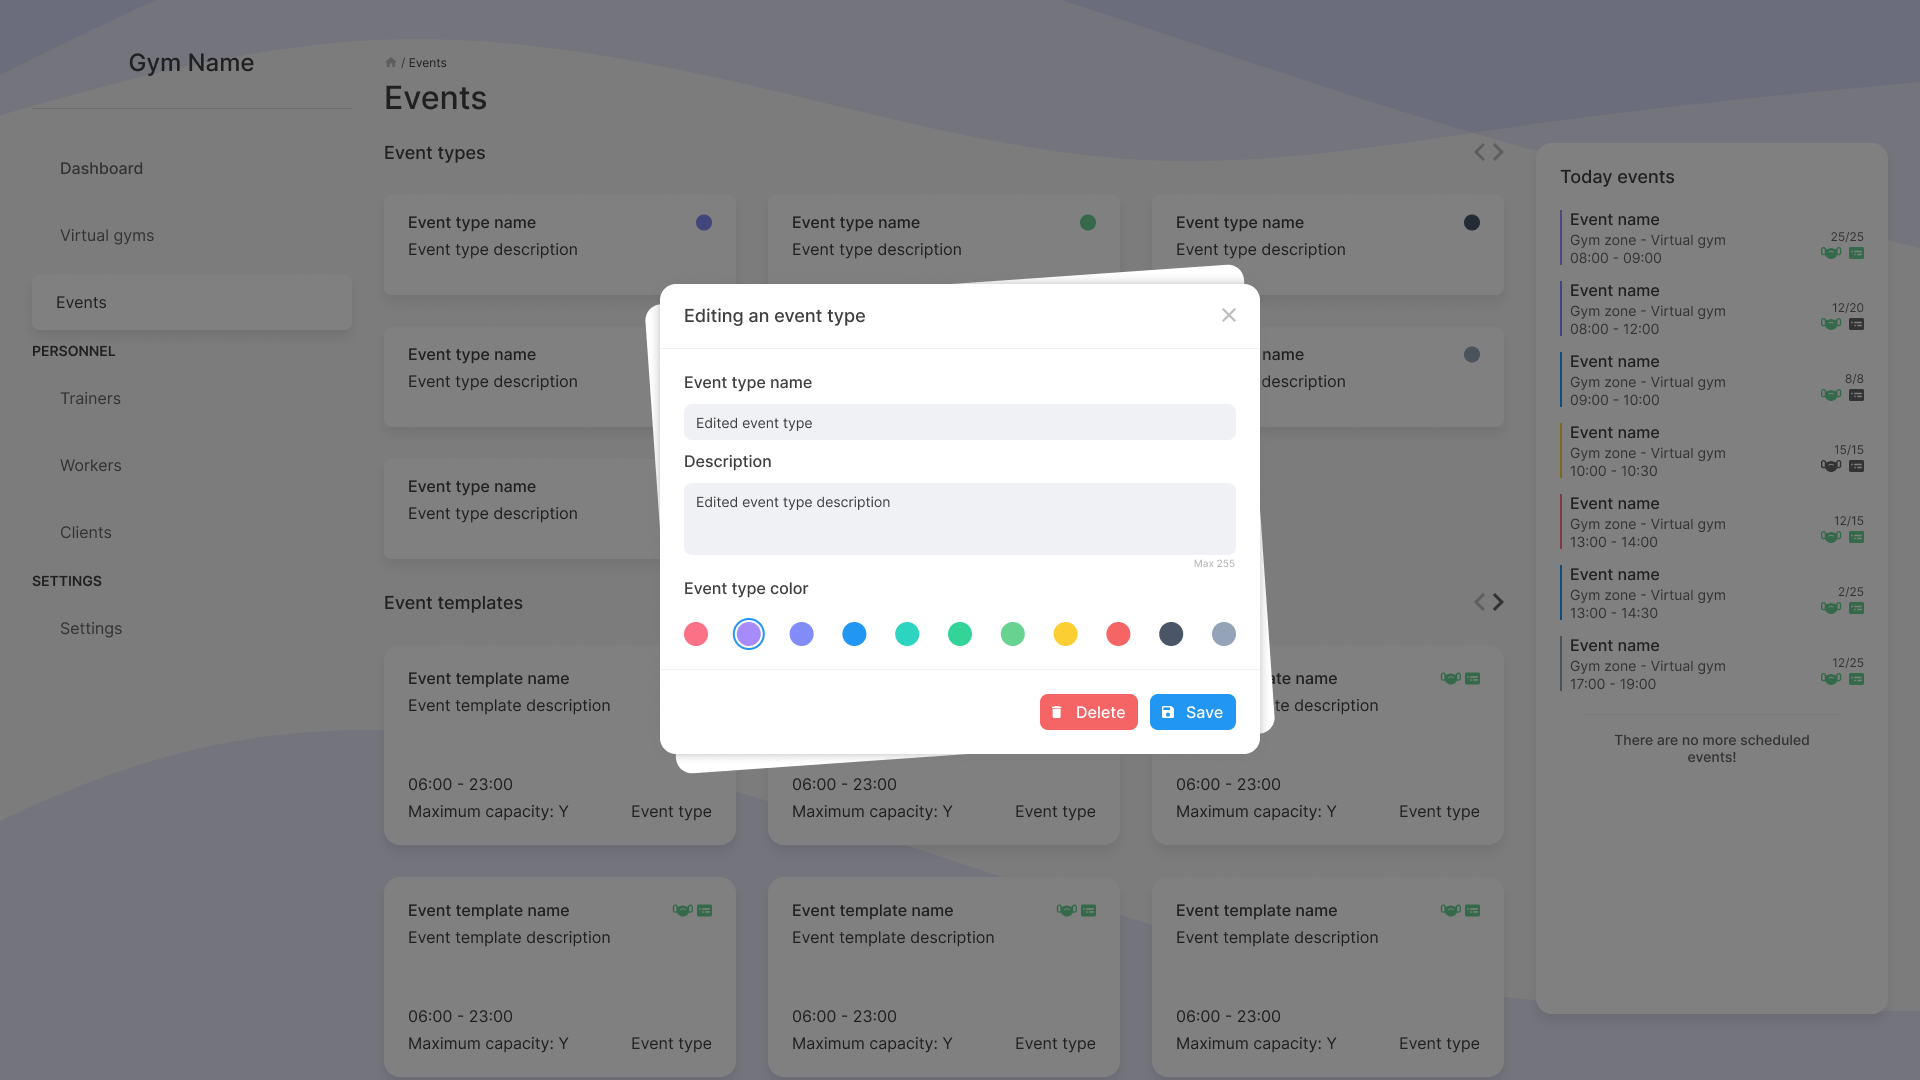
\includegraphics[width=\textwidth]{assets/ui/EventTypeEdit.png}
	\caption{Event type dialog (edit state)}
\end{figure}
\begin{figure}[H]
	\centering
	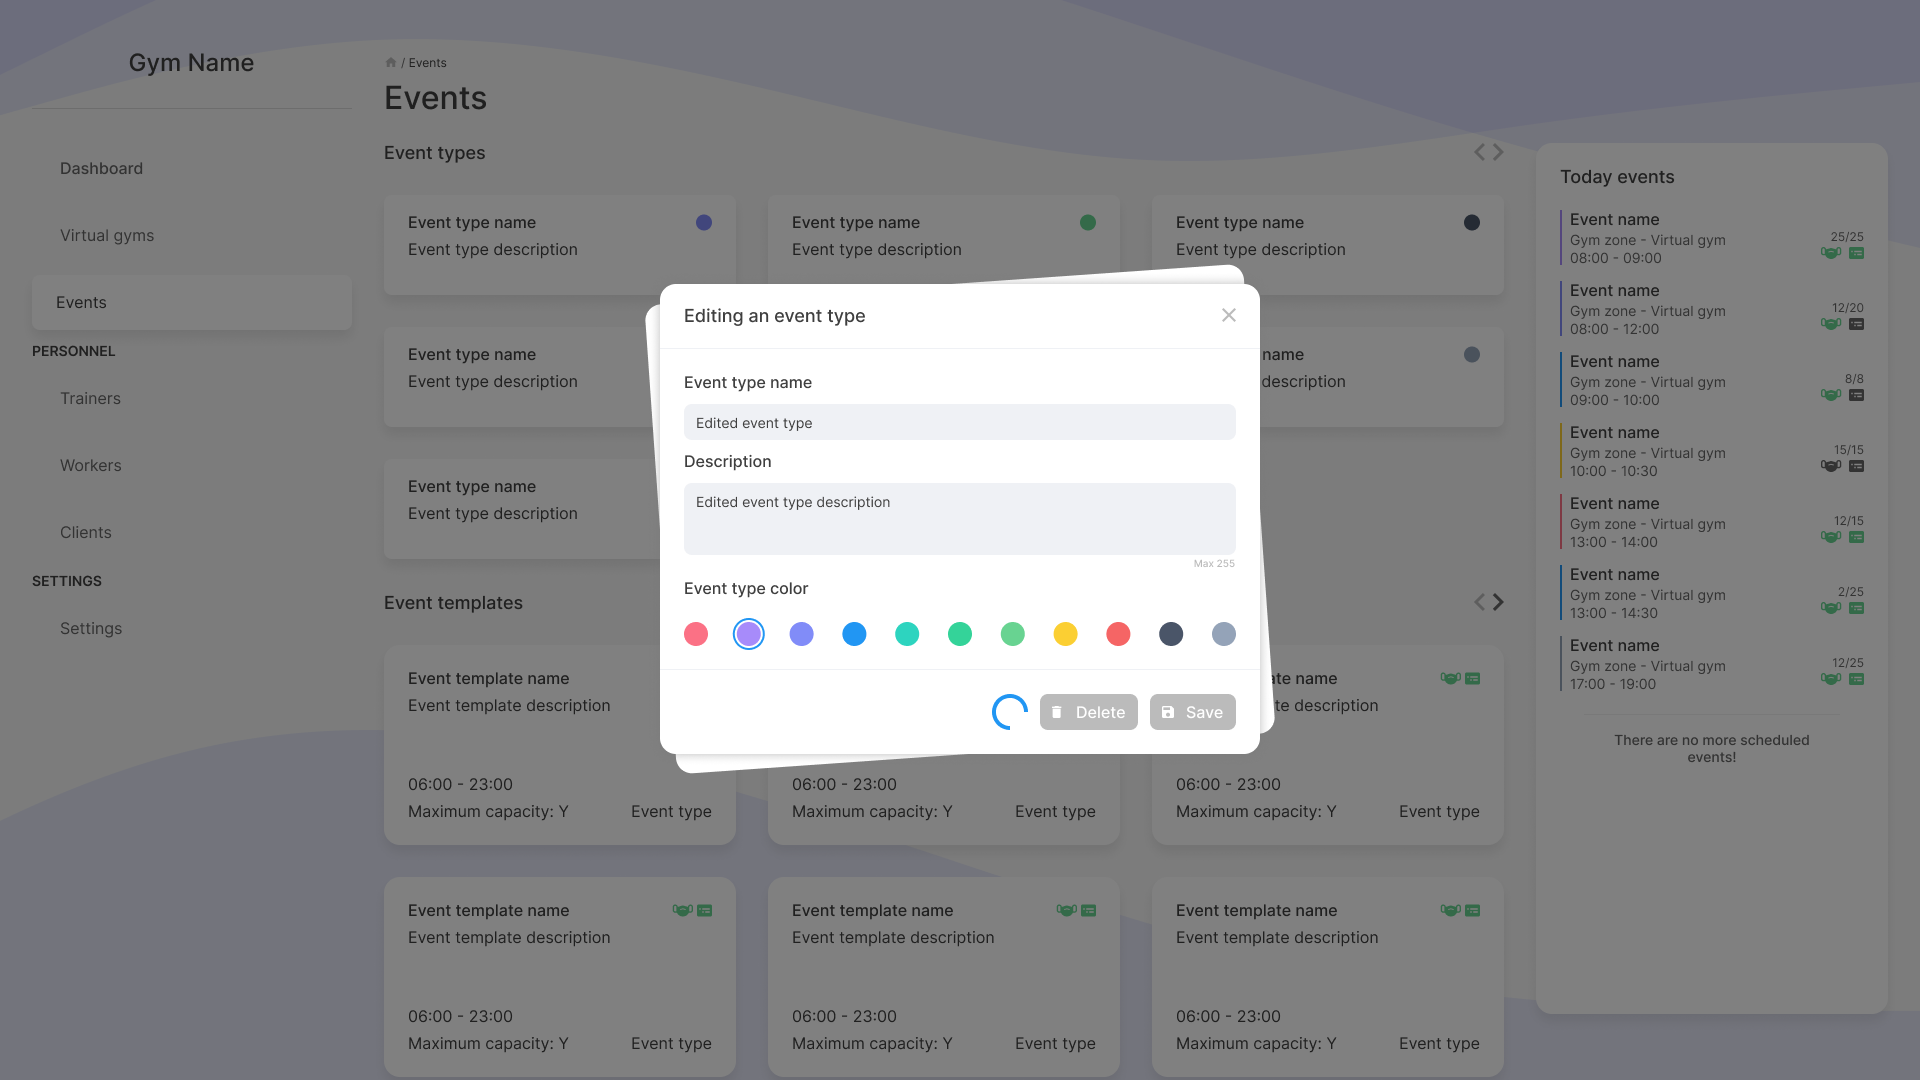
\includegraphics[width=\textwidth]{assets/ui/EventTypeEditLoading.png}
	\caption{Event type dialog (edit-loading state)}
\end{figure}
\begin{figure}[H]
	\centering
	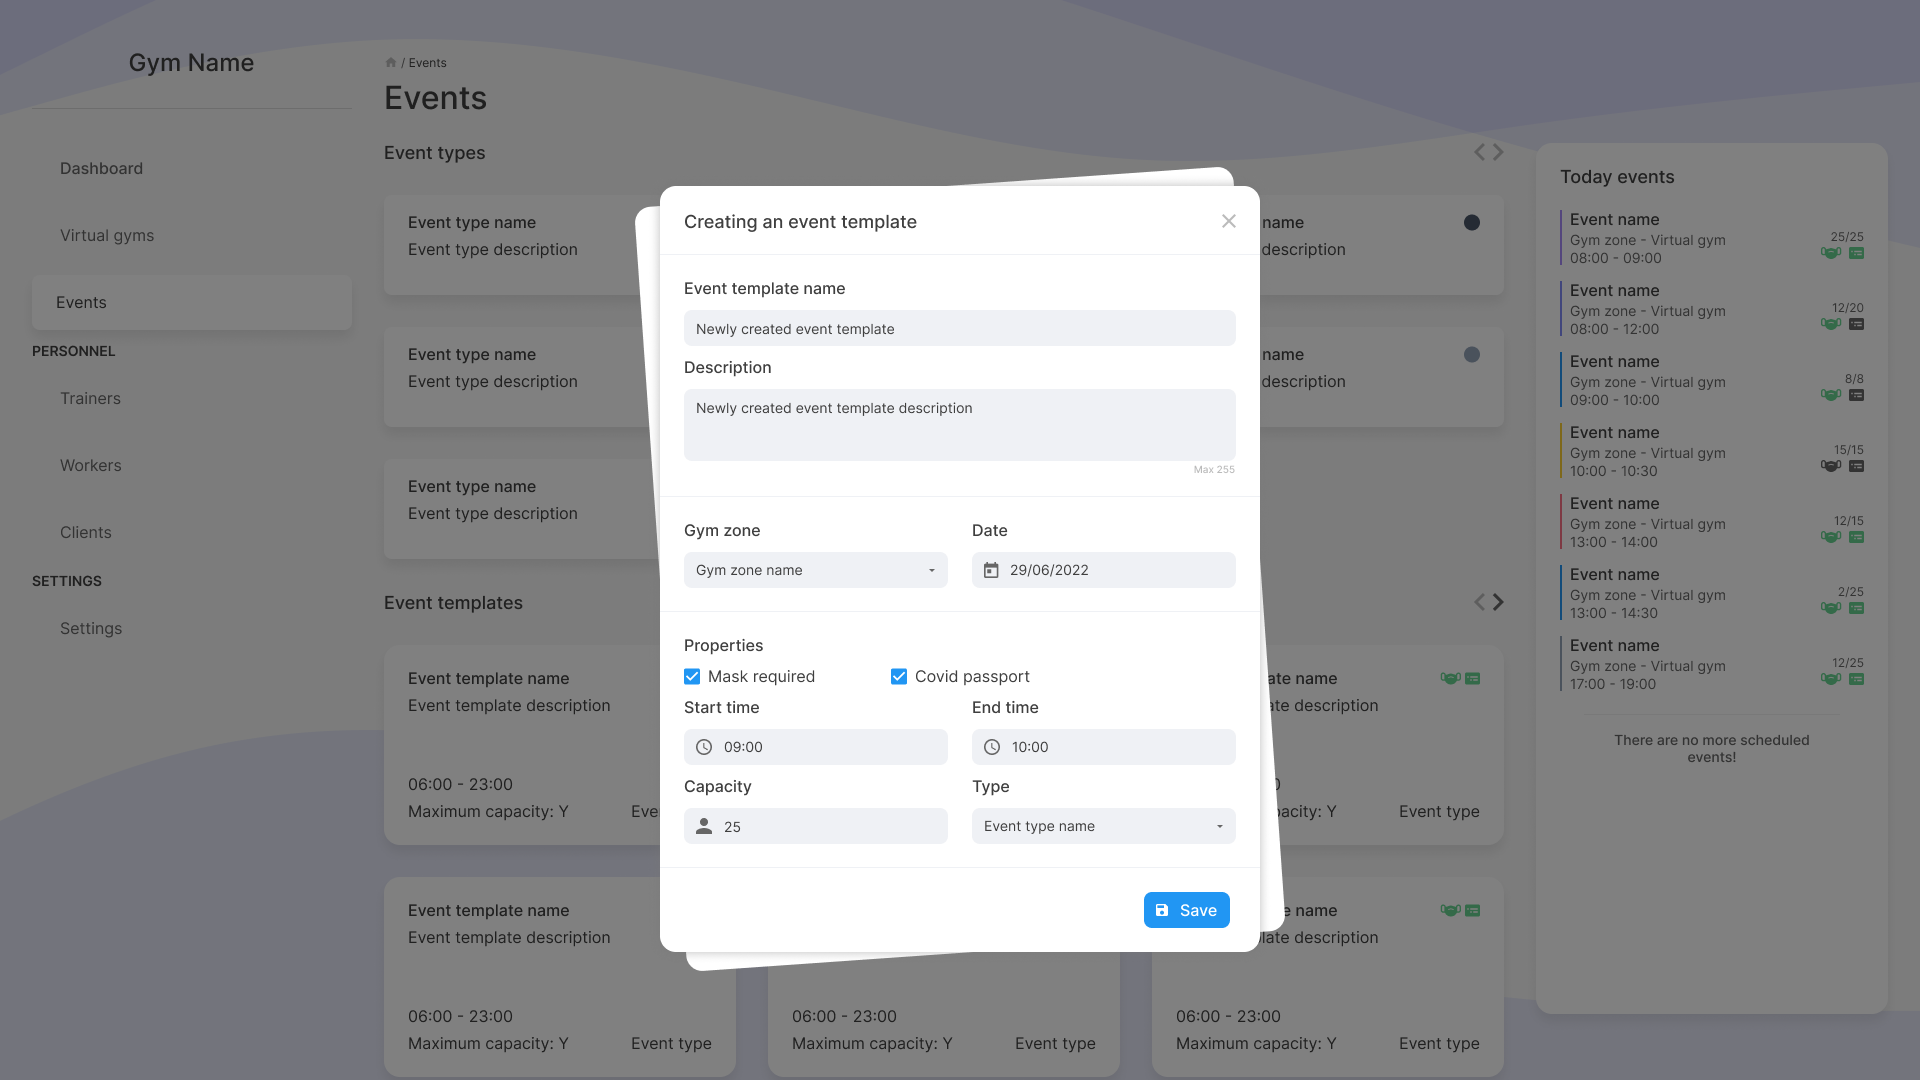
\includegraphics[width=\textwidth]{assets/ui/EventTemplateCreate.png}
	\caption{Event template dialog (create state)}
\end{figure}
\begin{figure}[H]
	\centering
	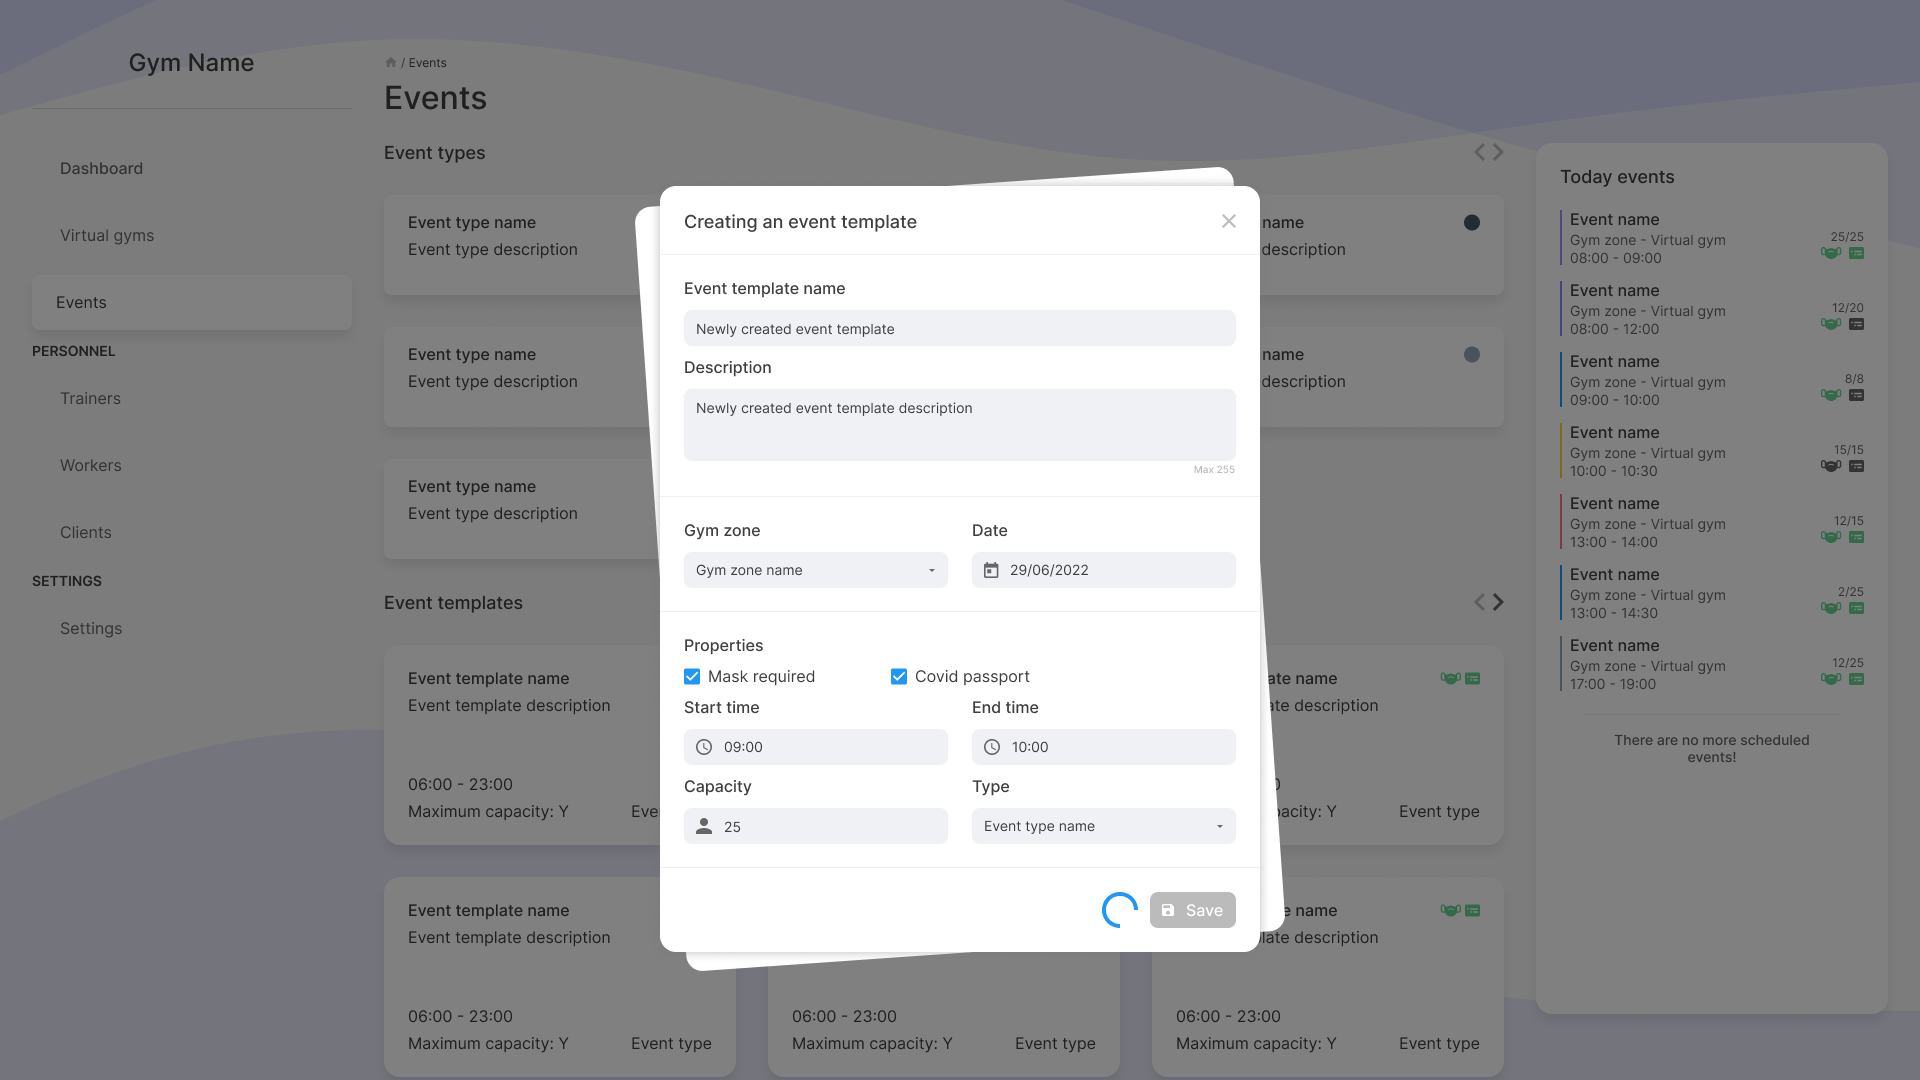
\includegraphics[width=\textwidth]{assets/ui/EventTemplateCreateLoading.png}
	\caption{Event template dialog (create-loading state)}
\end{figure}
\begin{figure}[H]
	\centering
	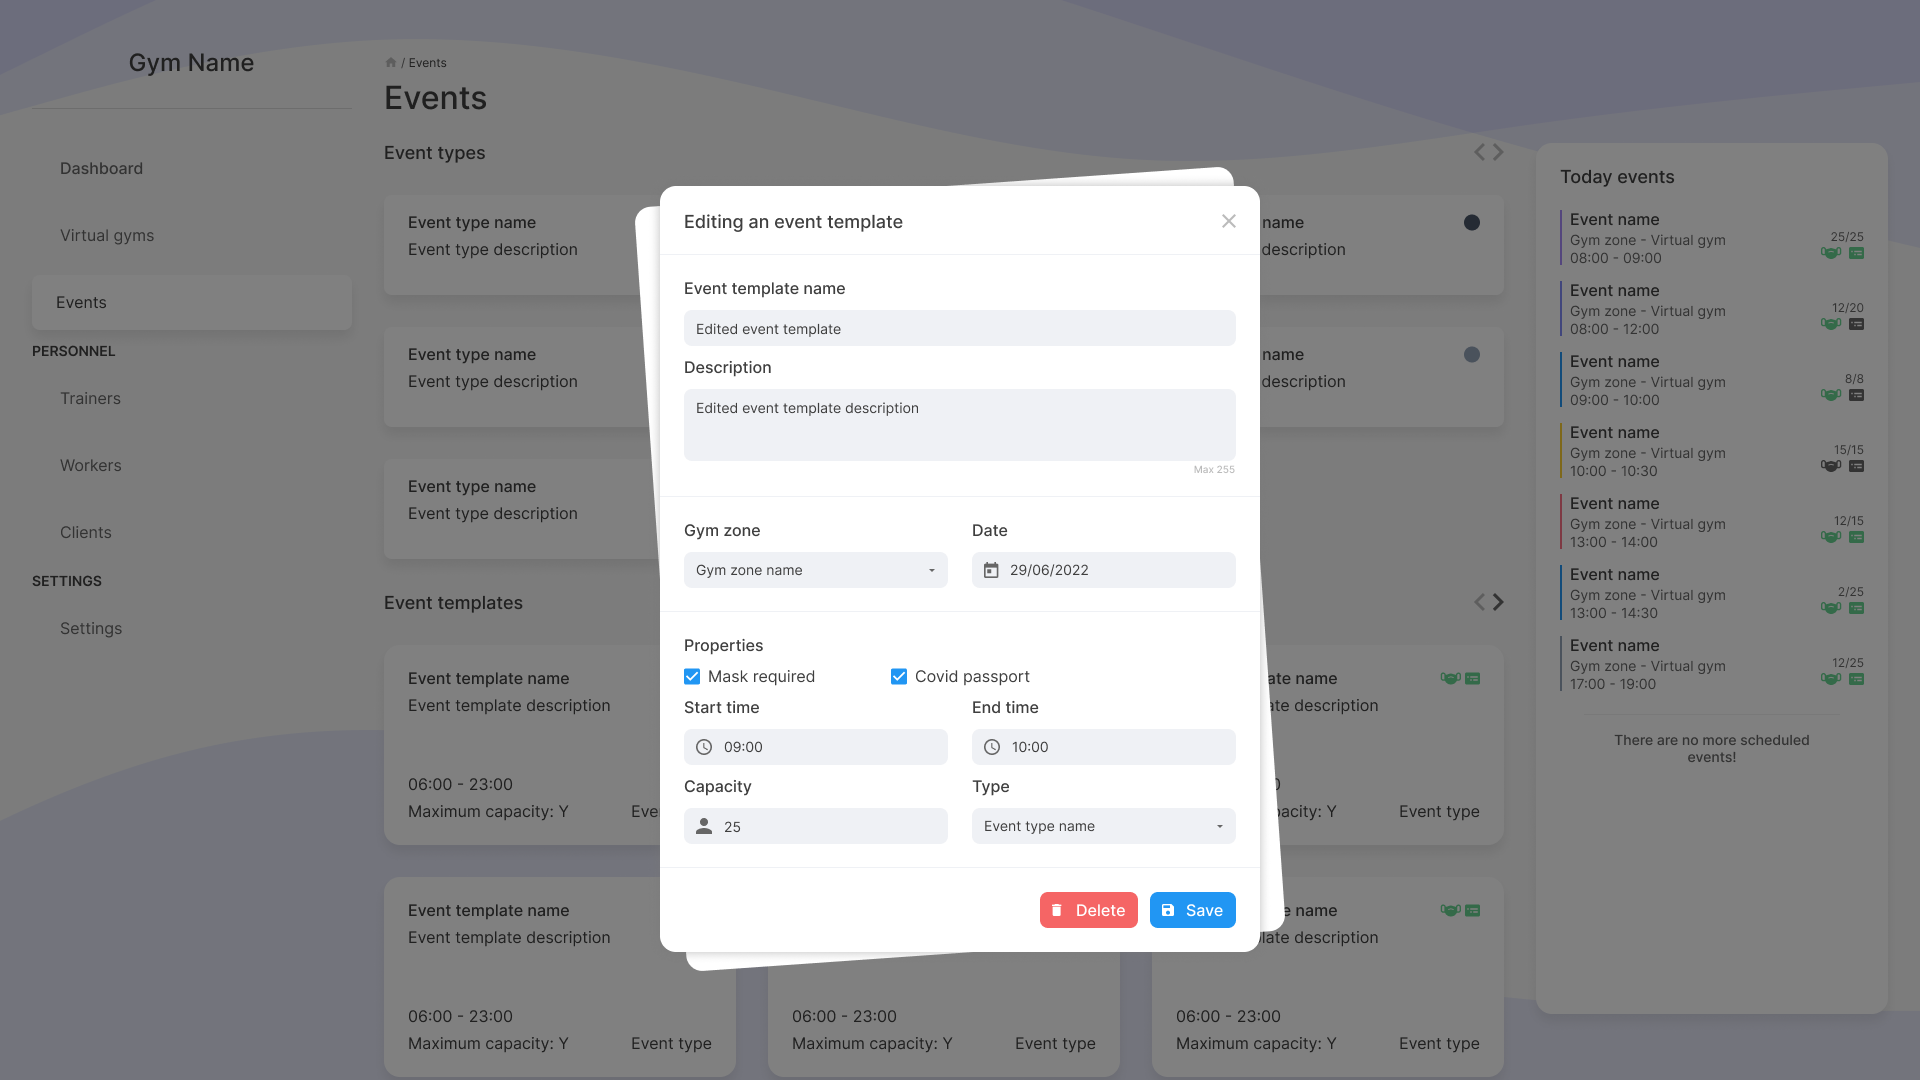
\includegraphics[width=\textwidth]{assets/ui/EventTemplateEdit.png}
	\caption{Event template dialog (edit state)}
\end{figure}
\begin{figure}[H]
	\centering
	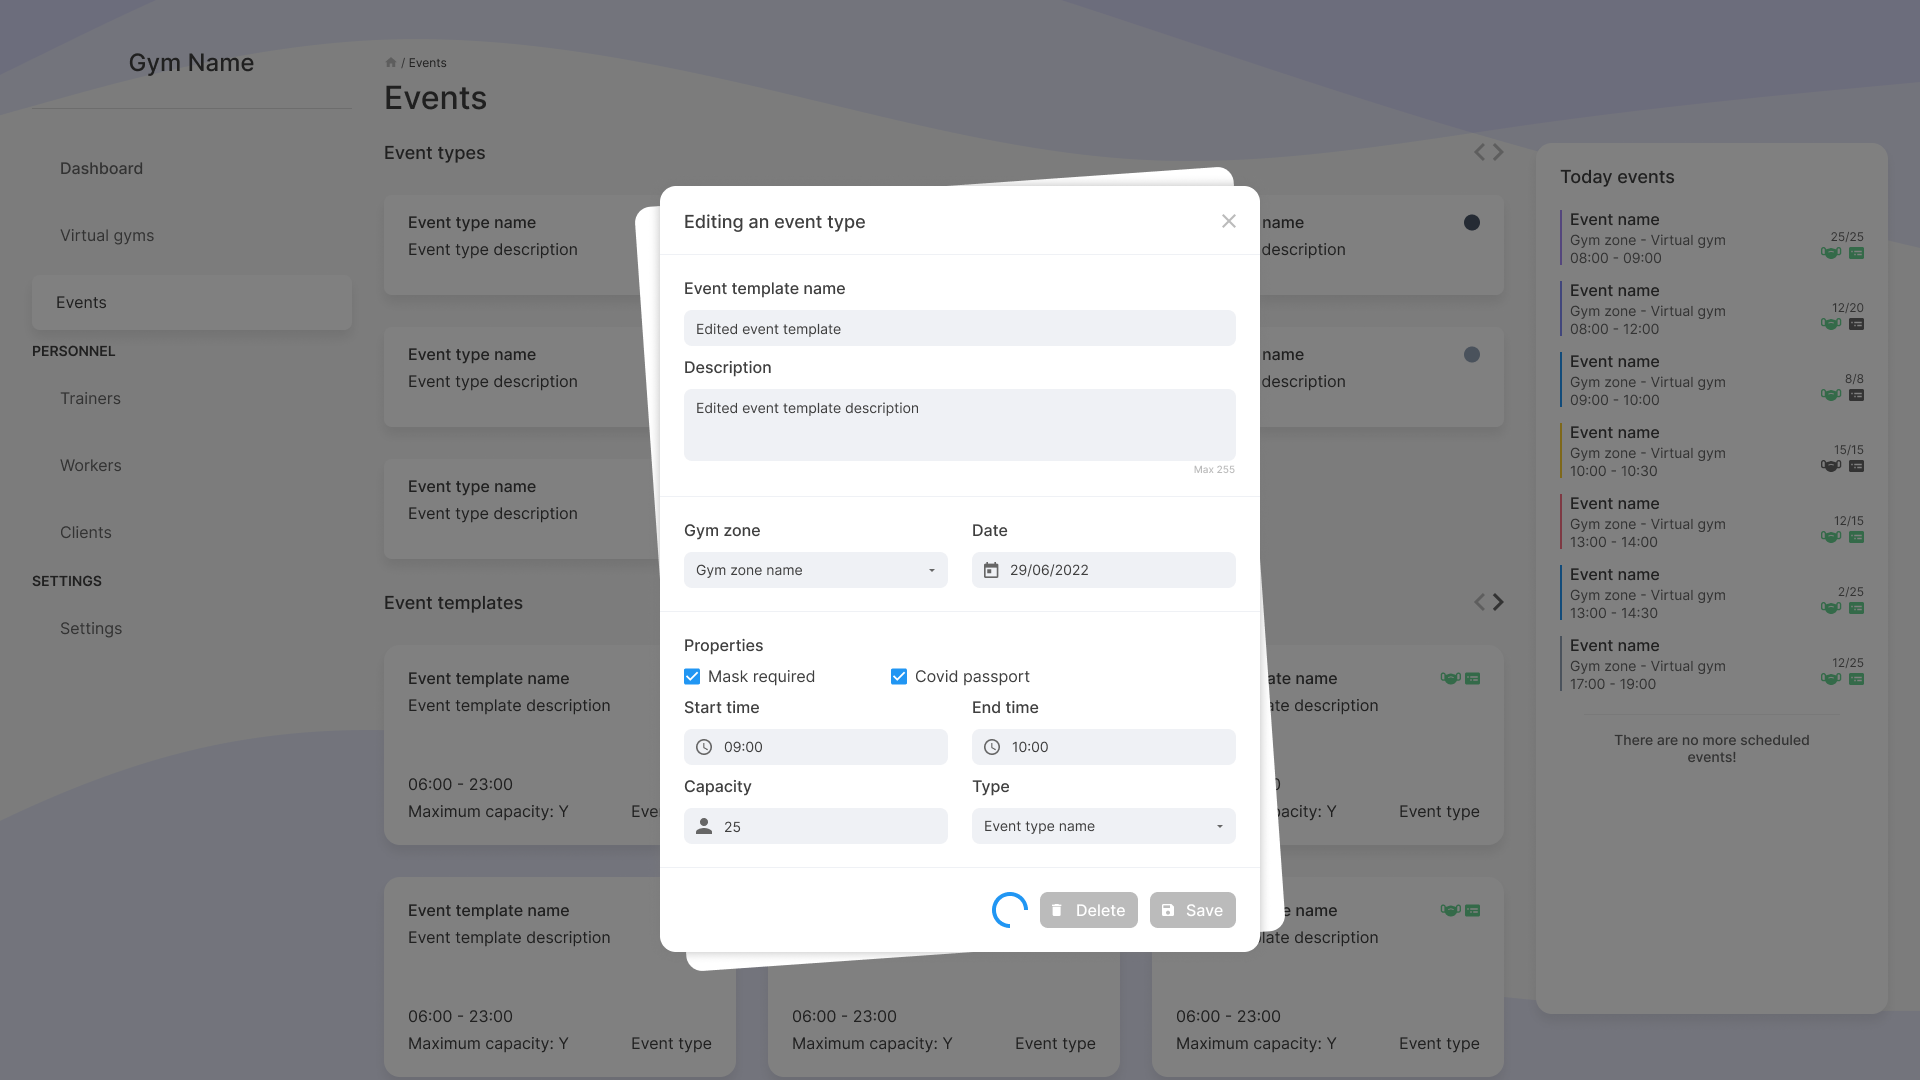
\includegraphics[width=\textwidth]{assets/ui/EventTemplateEditLoading.png}
	\caption{Event template dialog (edit-loading state)}
\end{figure}
\begin{figure}[H]
	\centering
	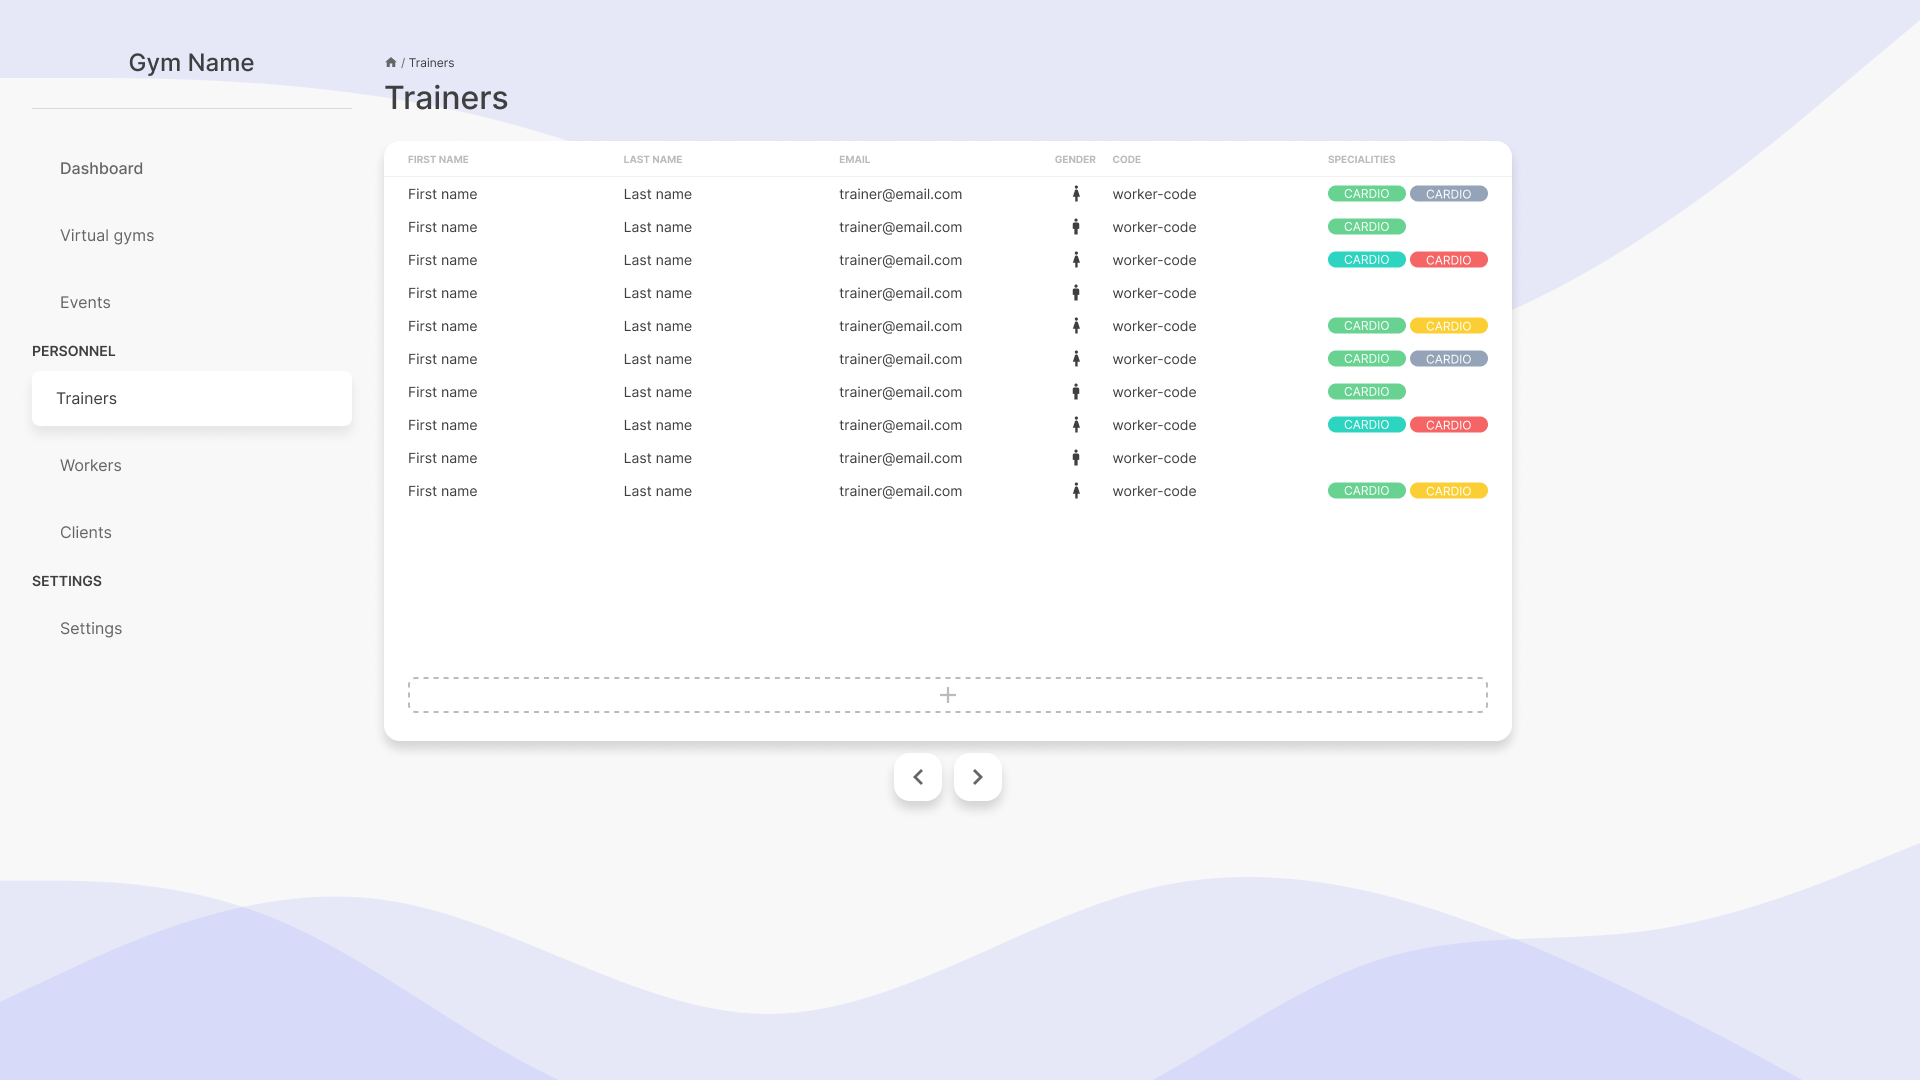
\includegraphics[width=\textwidth]{assets/ui/Trainers.png}
	\caption{Trainer's page, which is accessed using the left navigation bar}
\end{figure}
\begin{figure}[H]
	\centering
	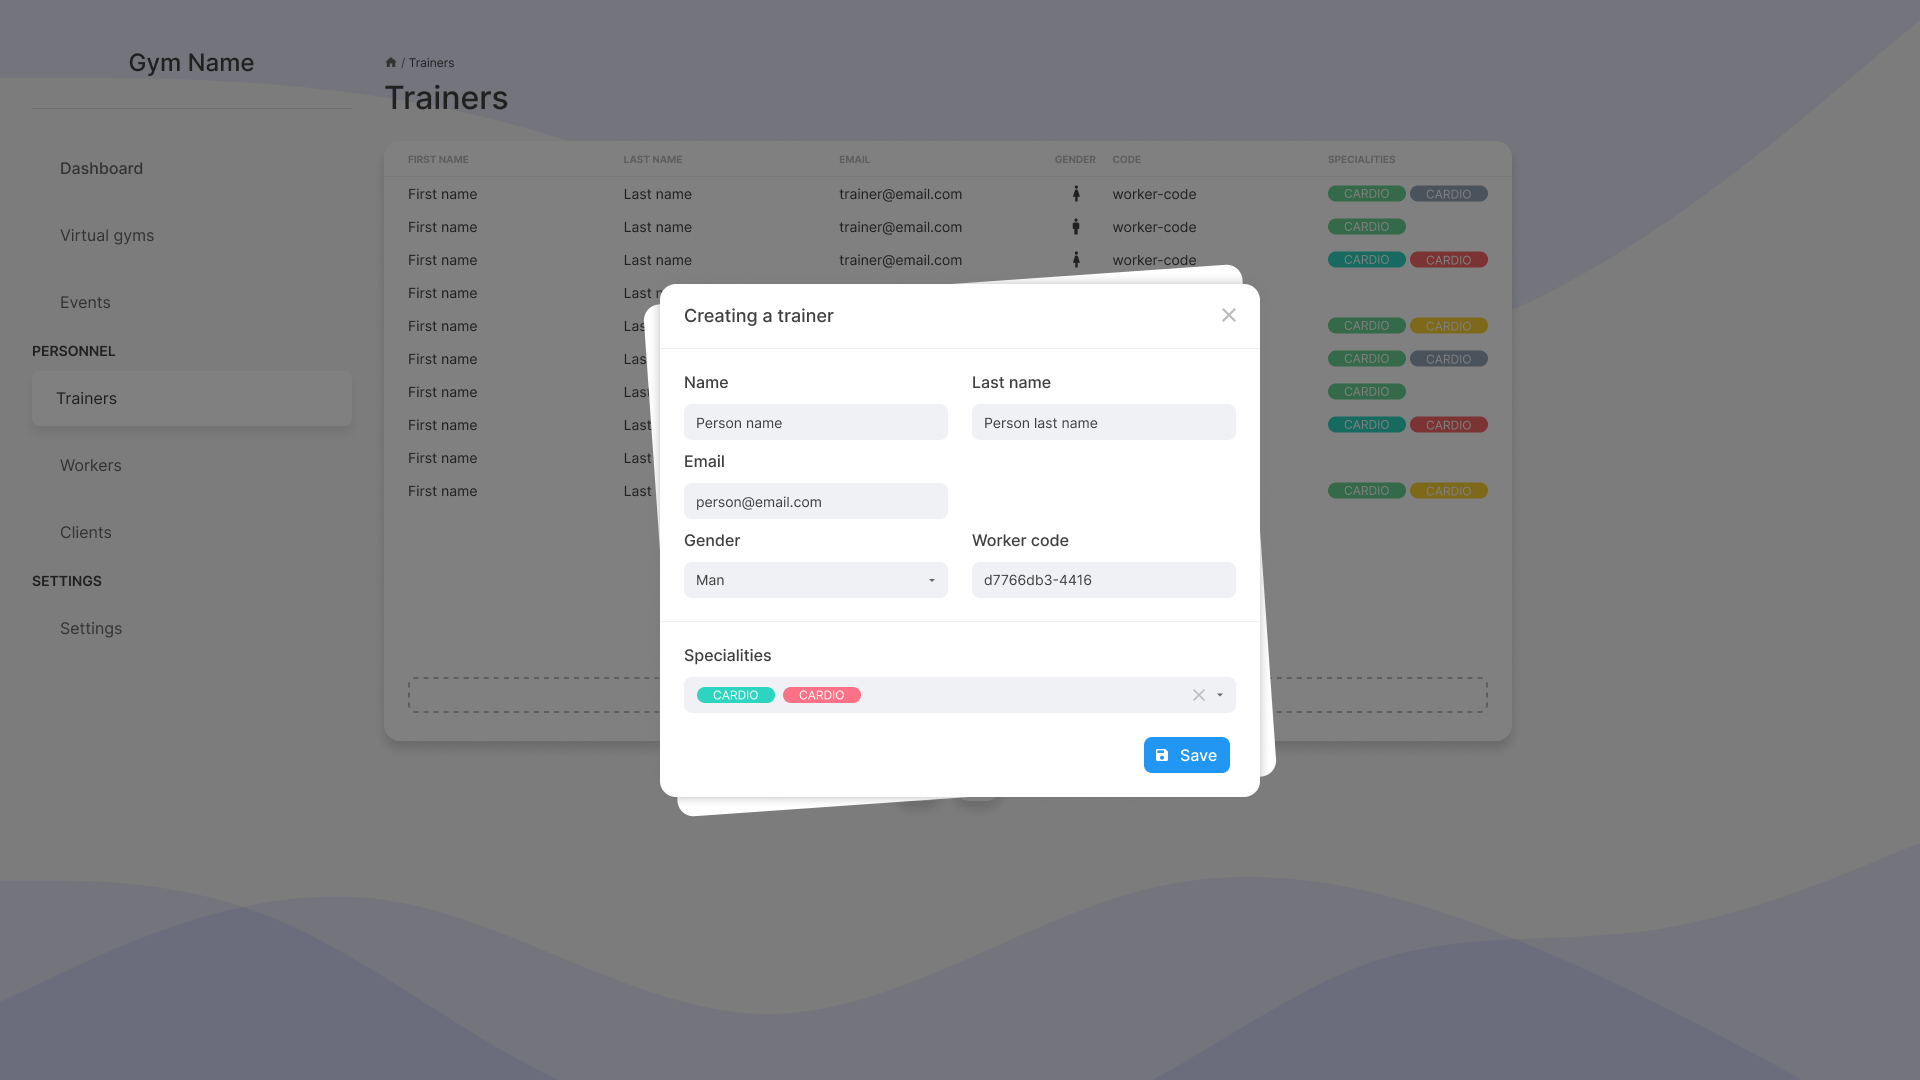
\includegraphics[width=\textwidth]{assets/ui/TrainerCreate.png}
	\caption{Trainer dialog (create state)}
\end{figure}
\begin{figure}[H]
	\centering
	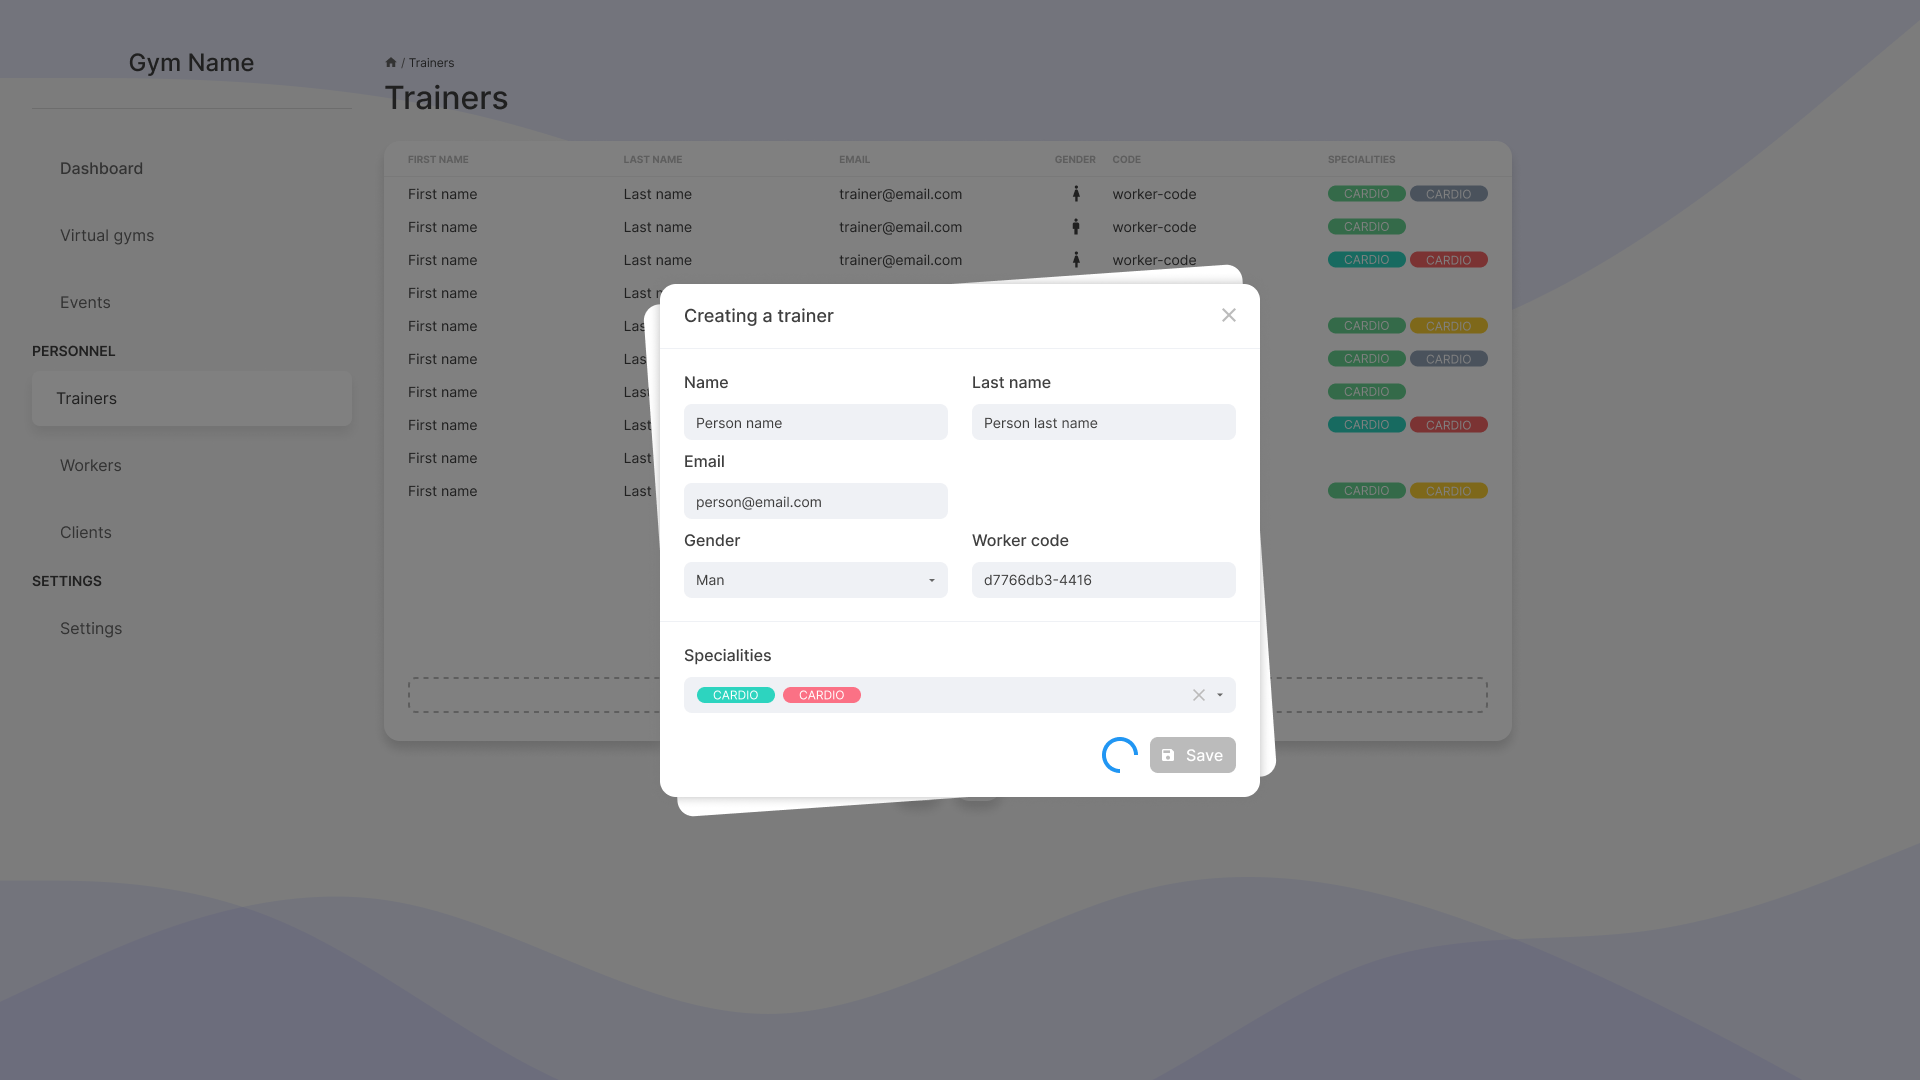
\includegraphics[width=\textwidth]{assets/ui/TrainerCreateLoading.png}
	\caption{Trainer dialog (create-edit state)}
\end{figure}
\begin{figure}[H]
	\centering
	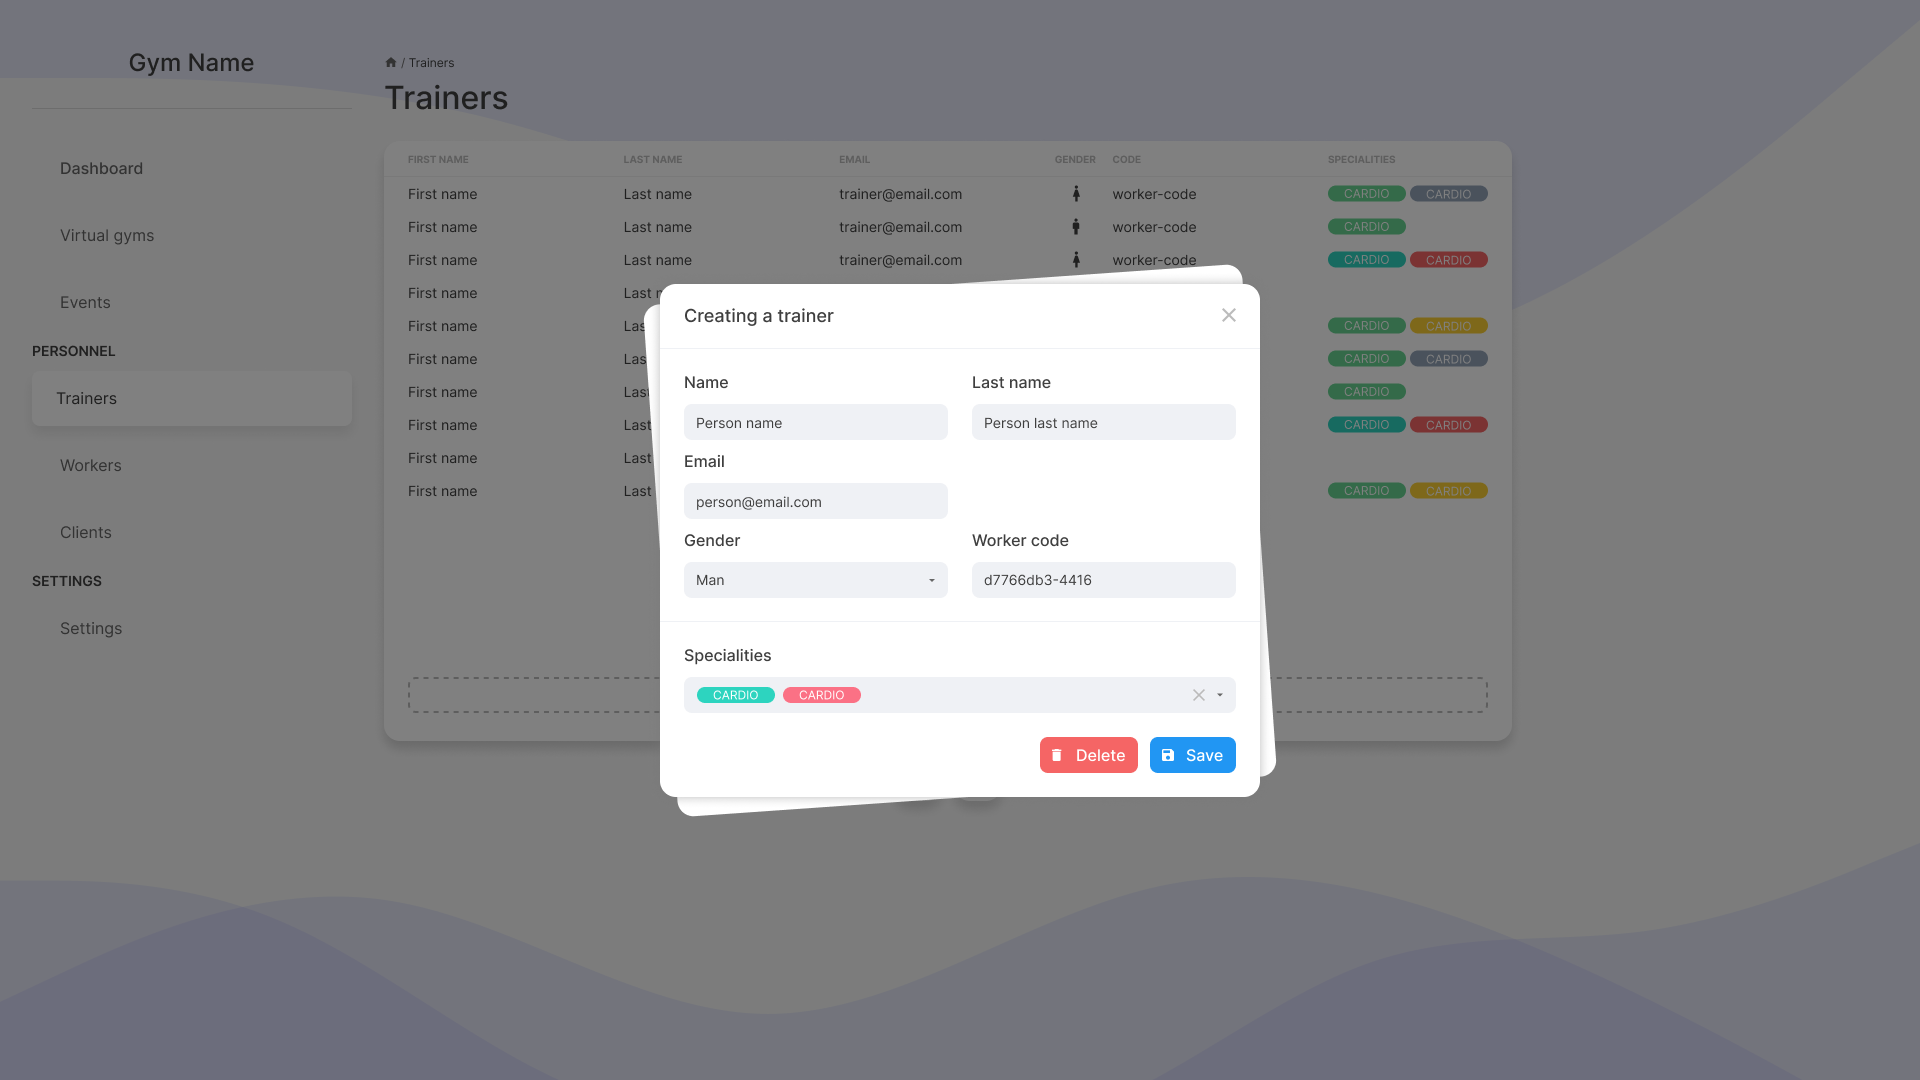
\includegraphics[width=\textwidth]{assets/ui/TrainerEdit.png}
	\caption{Trainer dialog (edit state)}
\end{figure}
\begin{figure}[H]
	\centering
	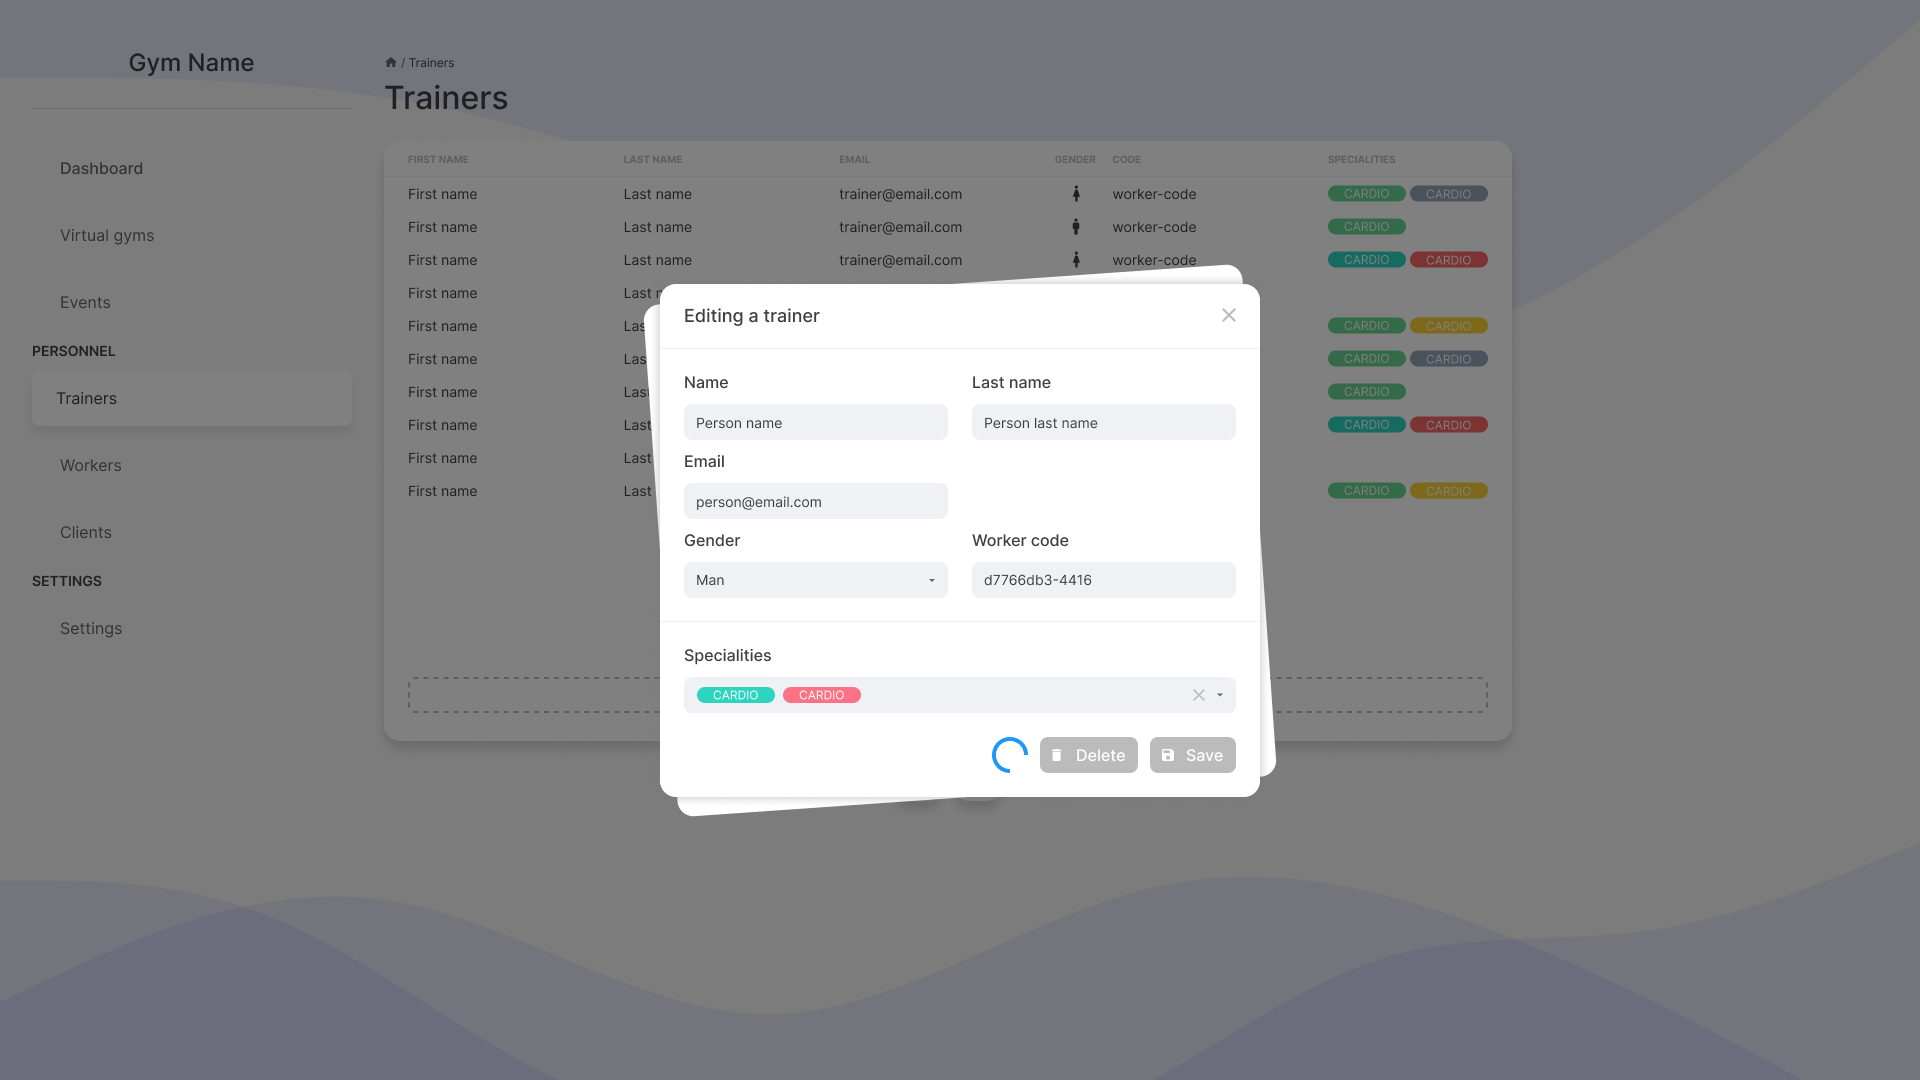
\includegraphics[width=\textwidth]{assets/ui/TrainerEditLoading.png}
	\caption{Trainer dialog (edit-loading state)}
\end{figure}
\begin{figure}[H]
	\centering
	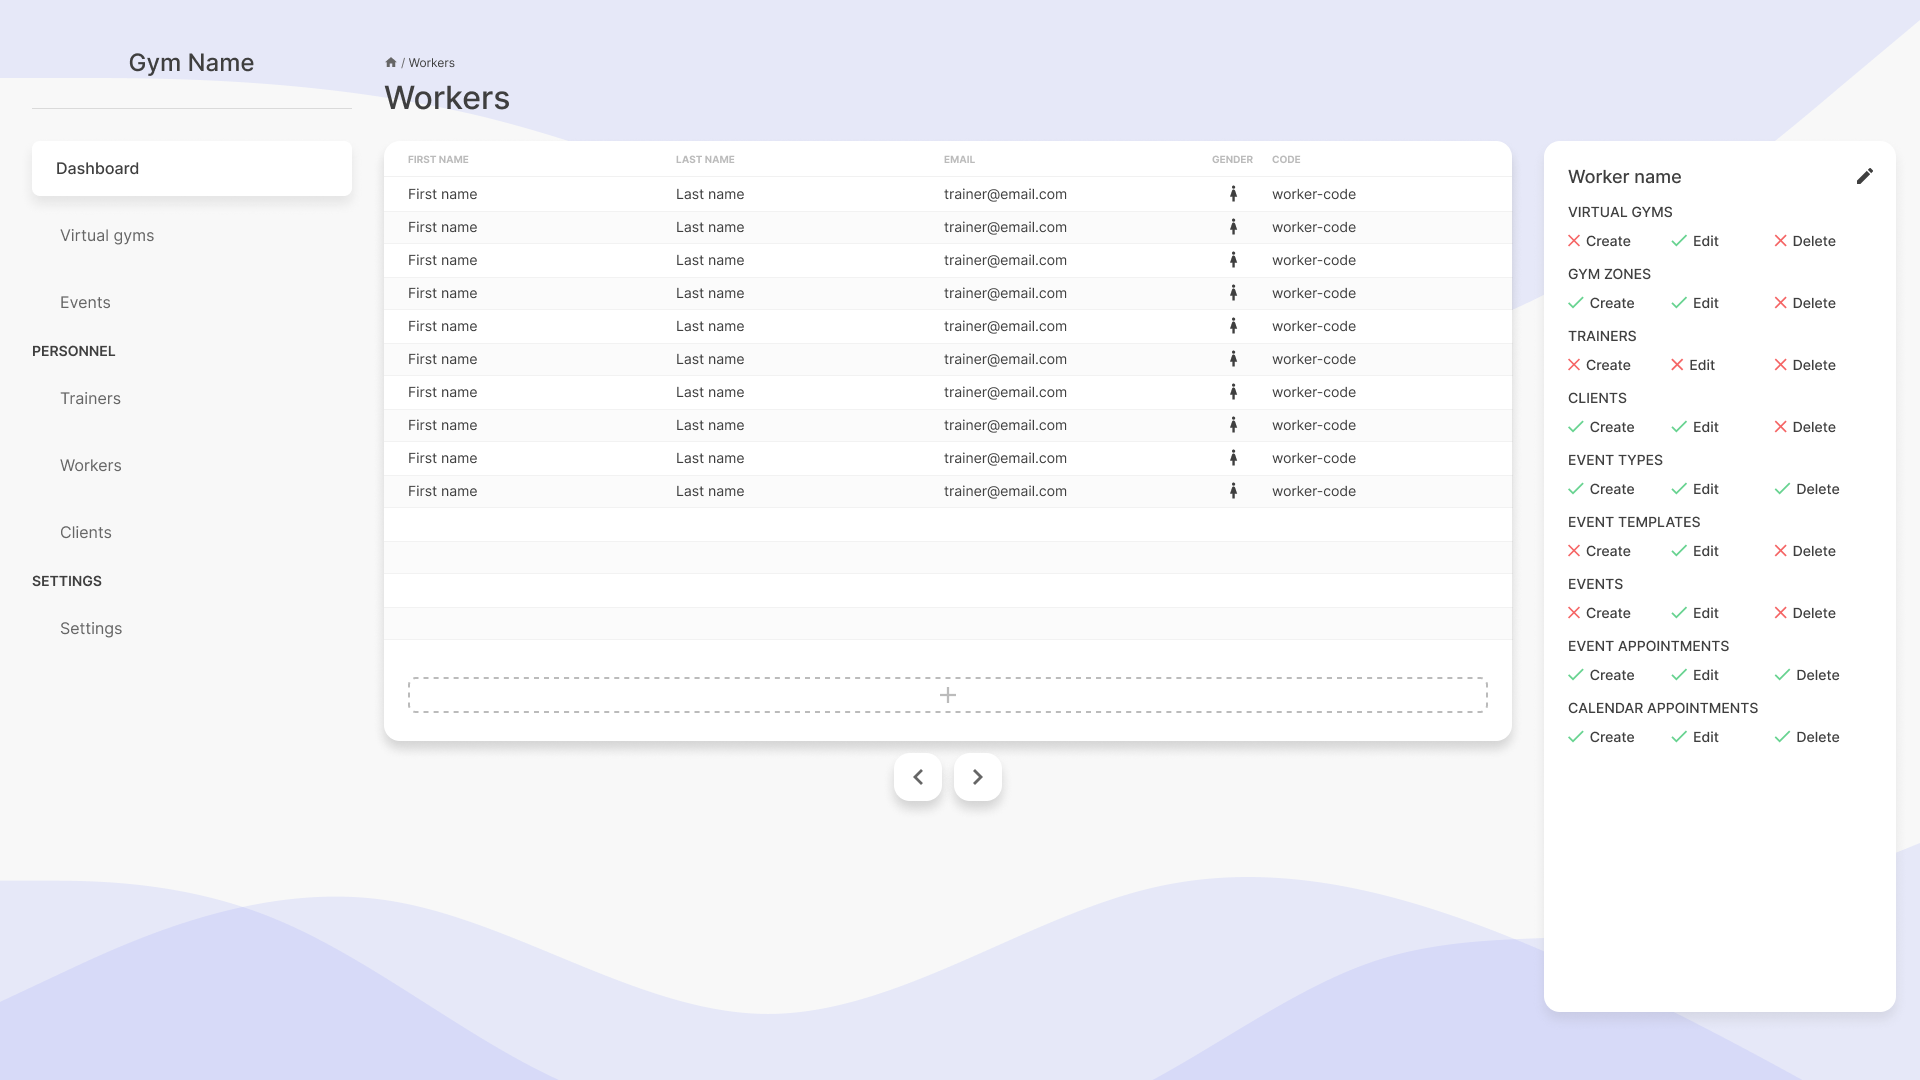
\includegraphics[width=\textwidth]{assets/ui/WorkersSelected.png}
	\caption{Worker's page, which is accessed using the left navigation bar}
\end{figure}
\begin{figure}[H]
	\centering
	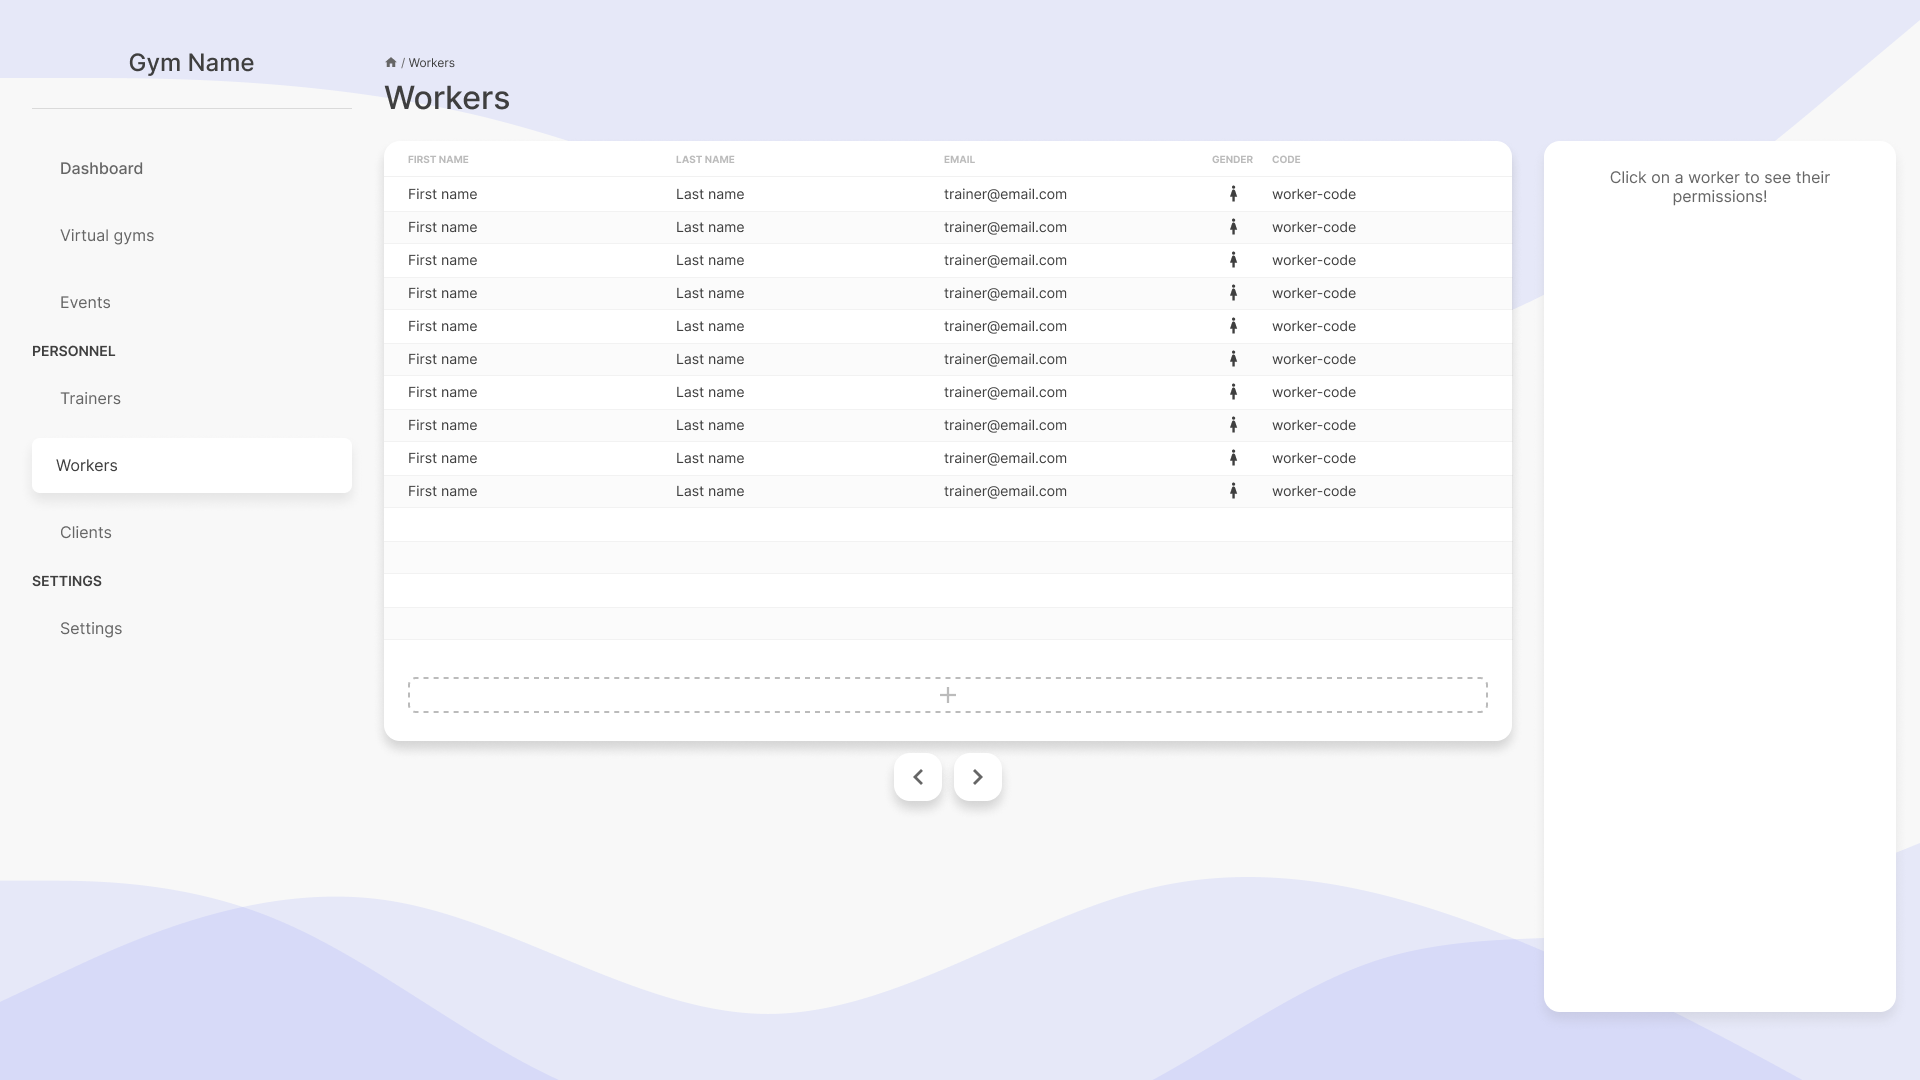
\includegraphics[width=\textwidth]{assets/ui/WorkersUnselected.png}
	\caption{Same as previous, with a selected worker}
\end{figure}
\begin{figure}[H]
	\centering
	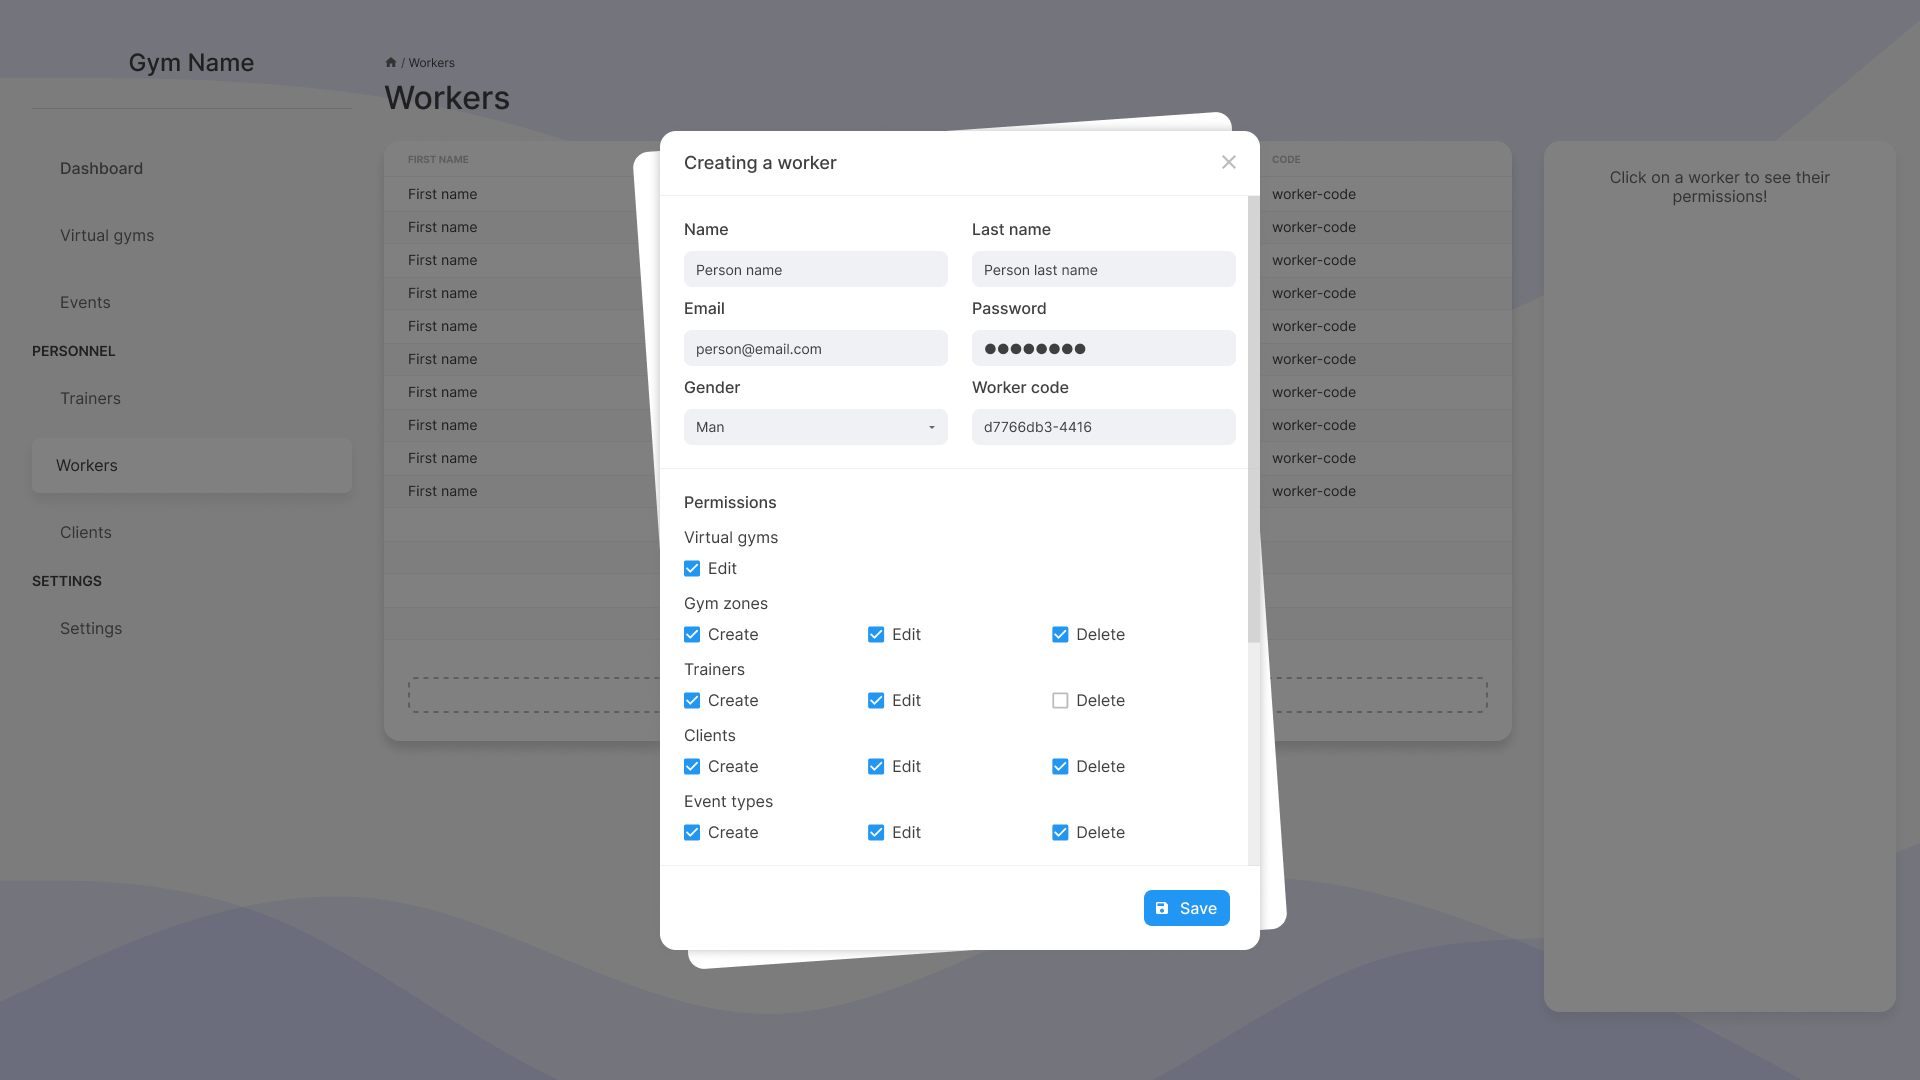
\includegraphics[width=\textwidth]{assets/ui/WorkersCreate.png}
	\caption{Worker dialog (create state)}
\end{figure}
\begin{figure}[H]
	\centering
	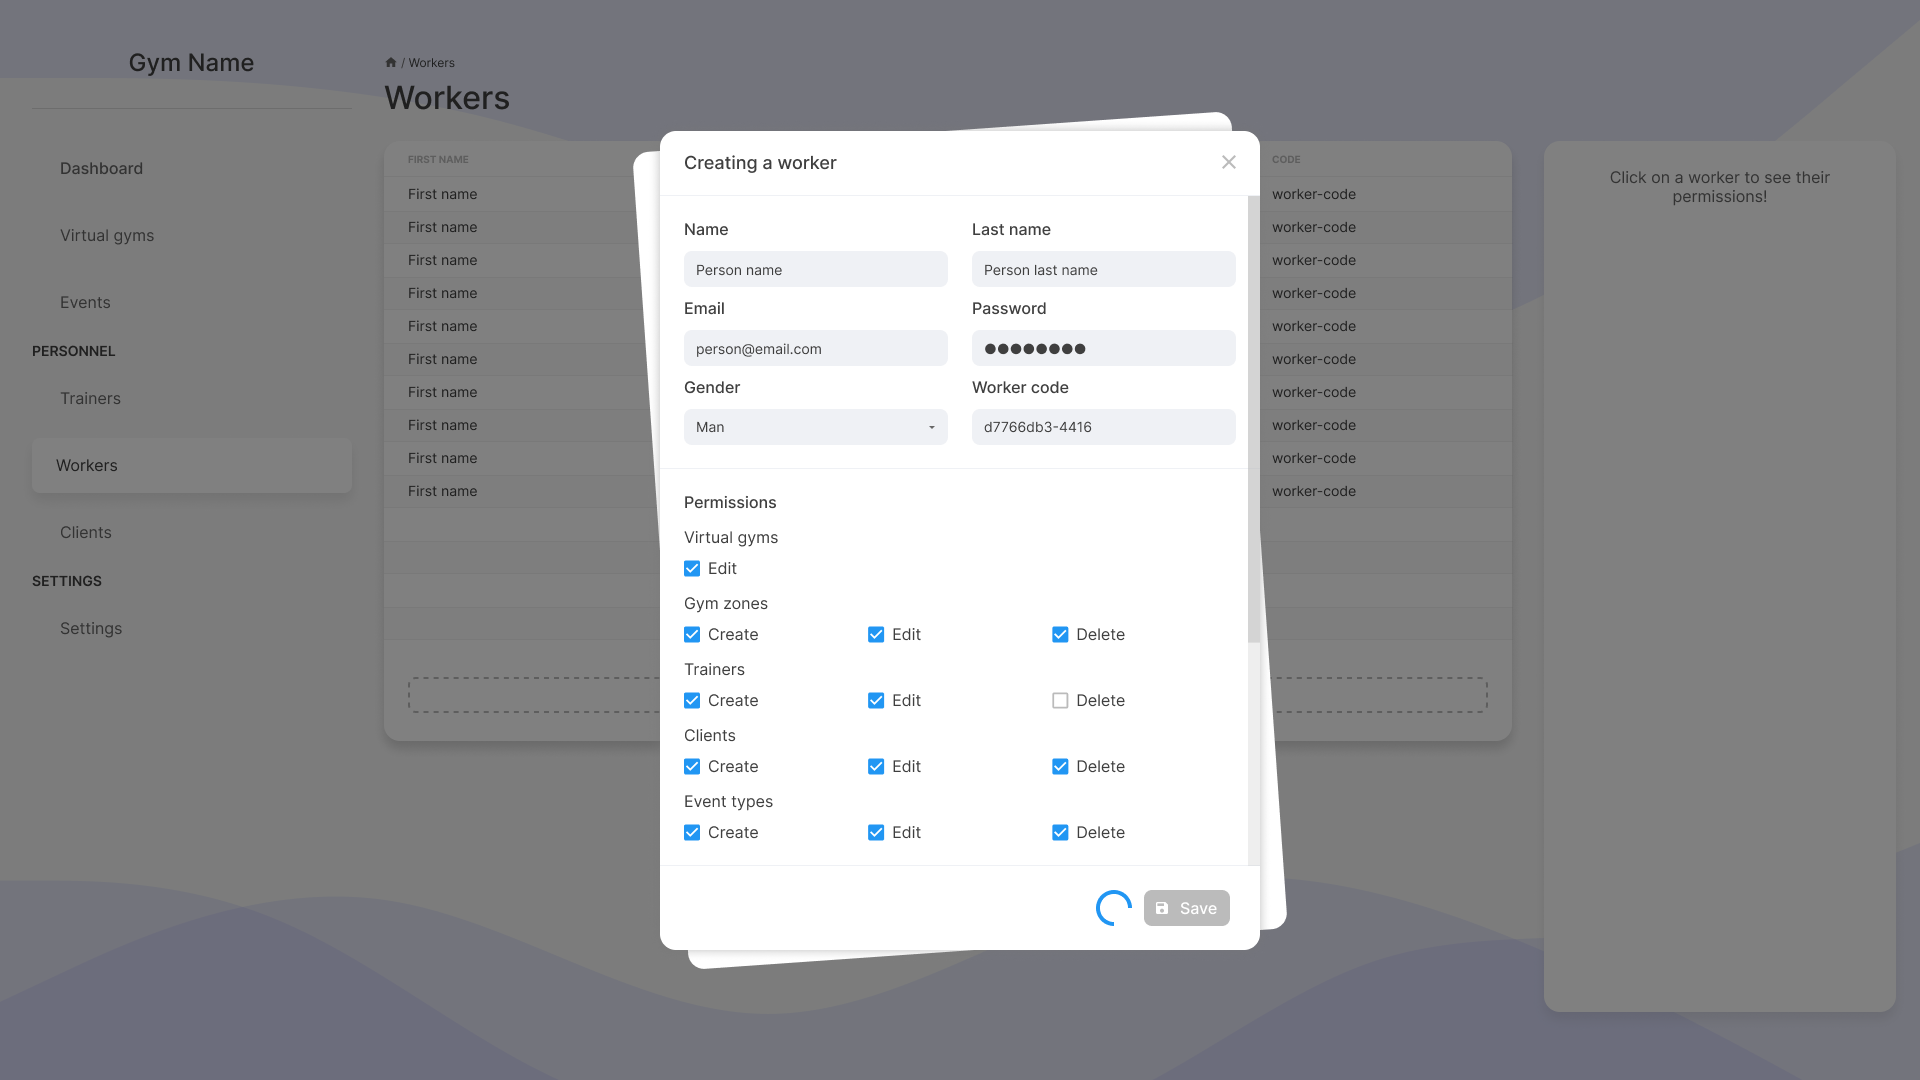
\includegraphics[width=\textwidth]{assets/ui/WorkersCreateLoading.png}
	\caption{Worker dialog (create-loading state)}
\end{figure}
\begin{figure}[H]
	\centering
	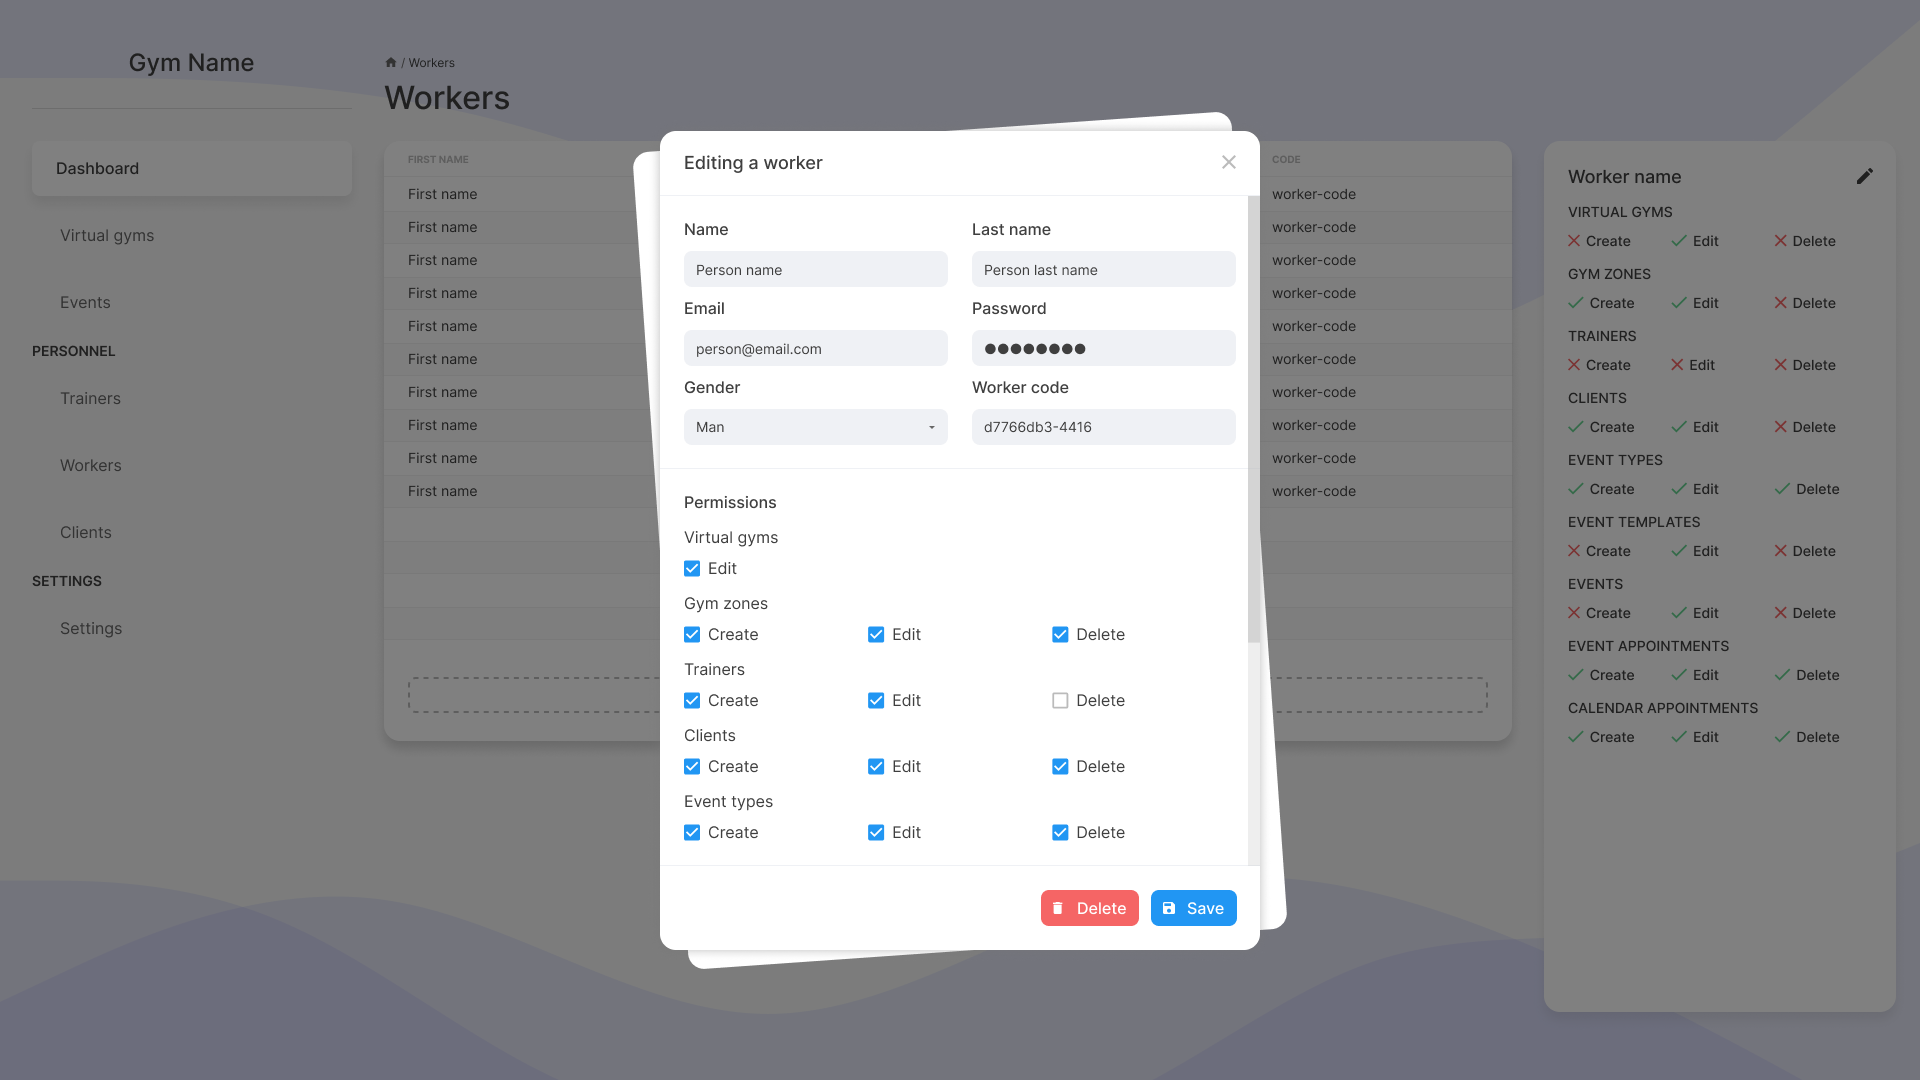
\includegraphics[width=\textwidth]{assets/ui/WorkersEdit.png}
	\caption{Worker dialog (edit state)}
\end{figure}
\begin{figure}[H]
	\centering
	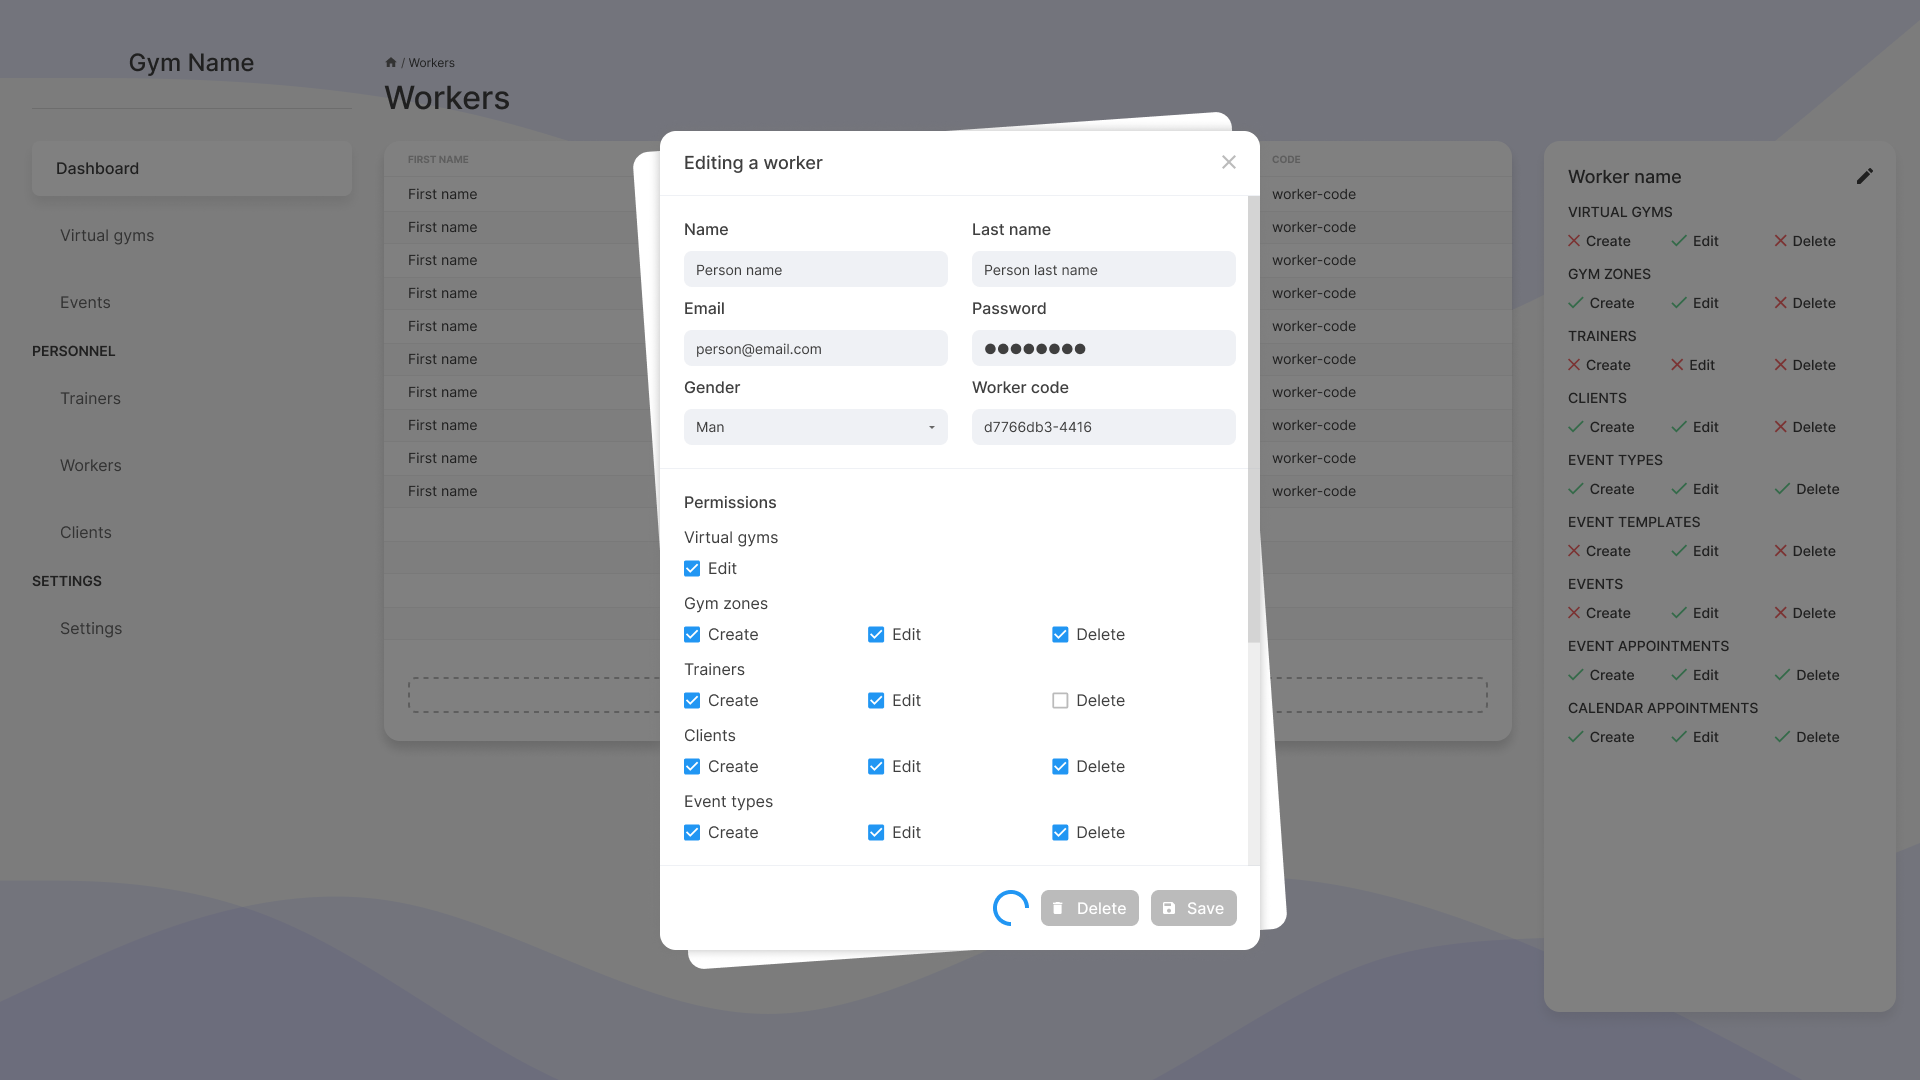
\includegraphics[width=\textwidth]{assets/ui/WorkersEditLoading.png}
	\caption{Worker dialog (edit-loading state)}
\end{figure}
\begin{figure}[H]
	\centering
	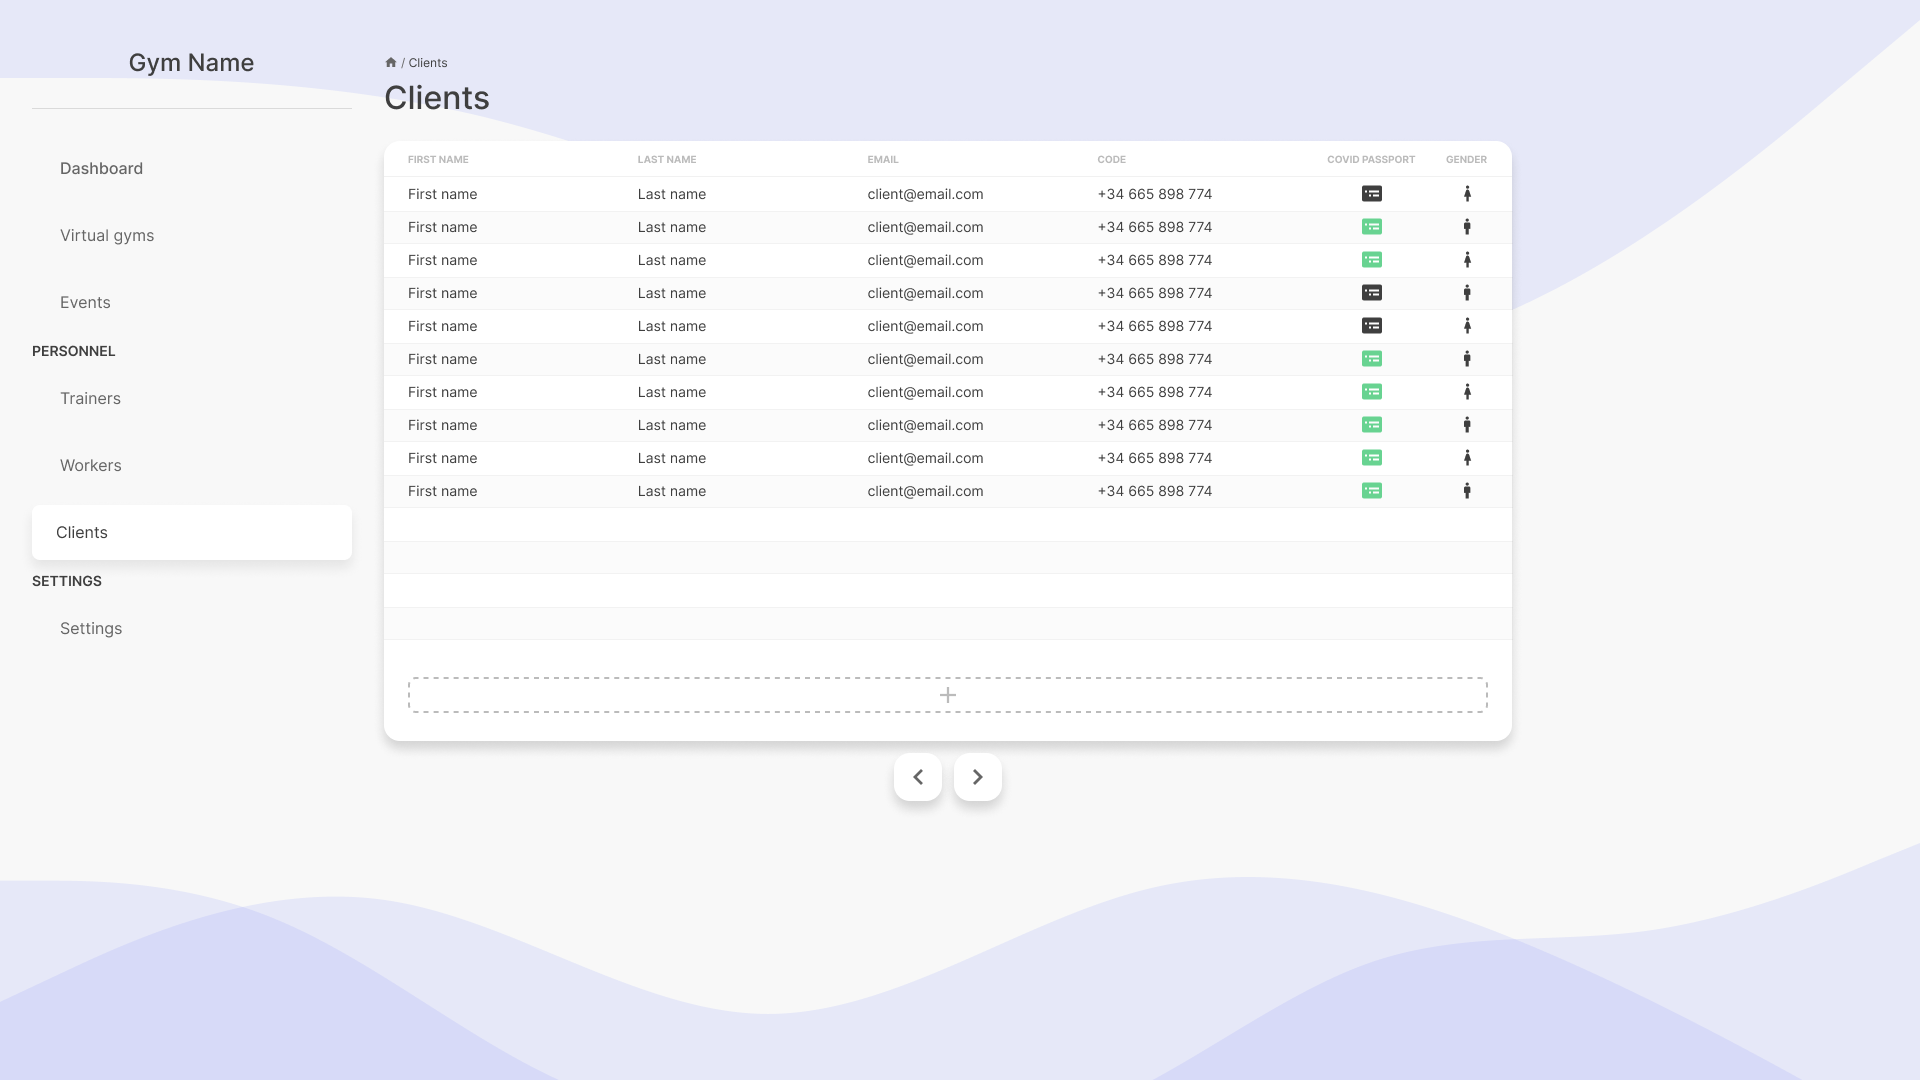
\includegraphics[width=\textwidth]{assets/ui/Clients.png}
	\caption{Client's page, which is accessed using the left navigation bar}
\end{figure}
\begin{figure}[H]
	\centering
	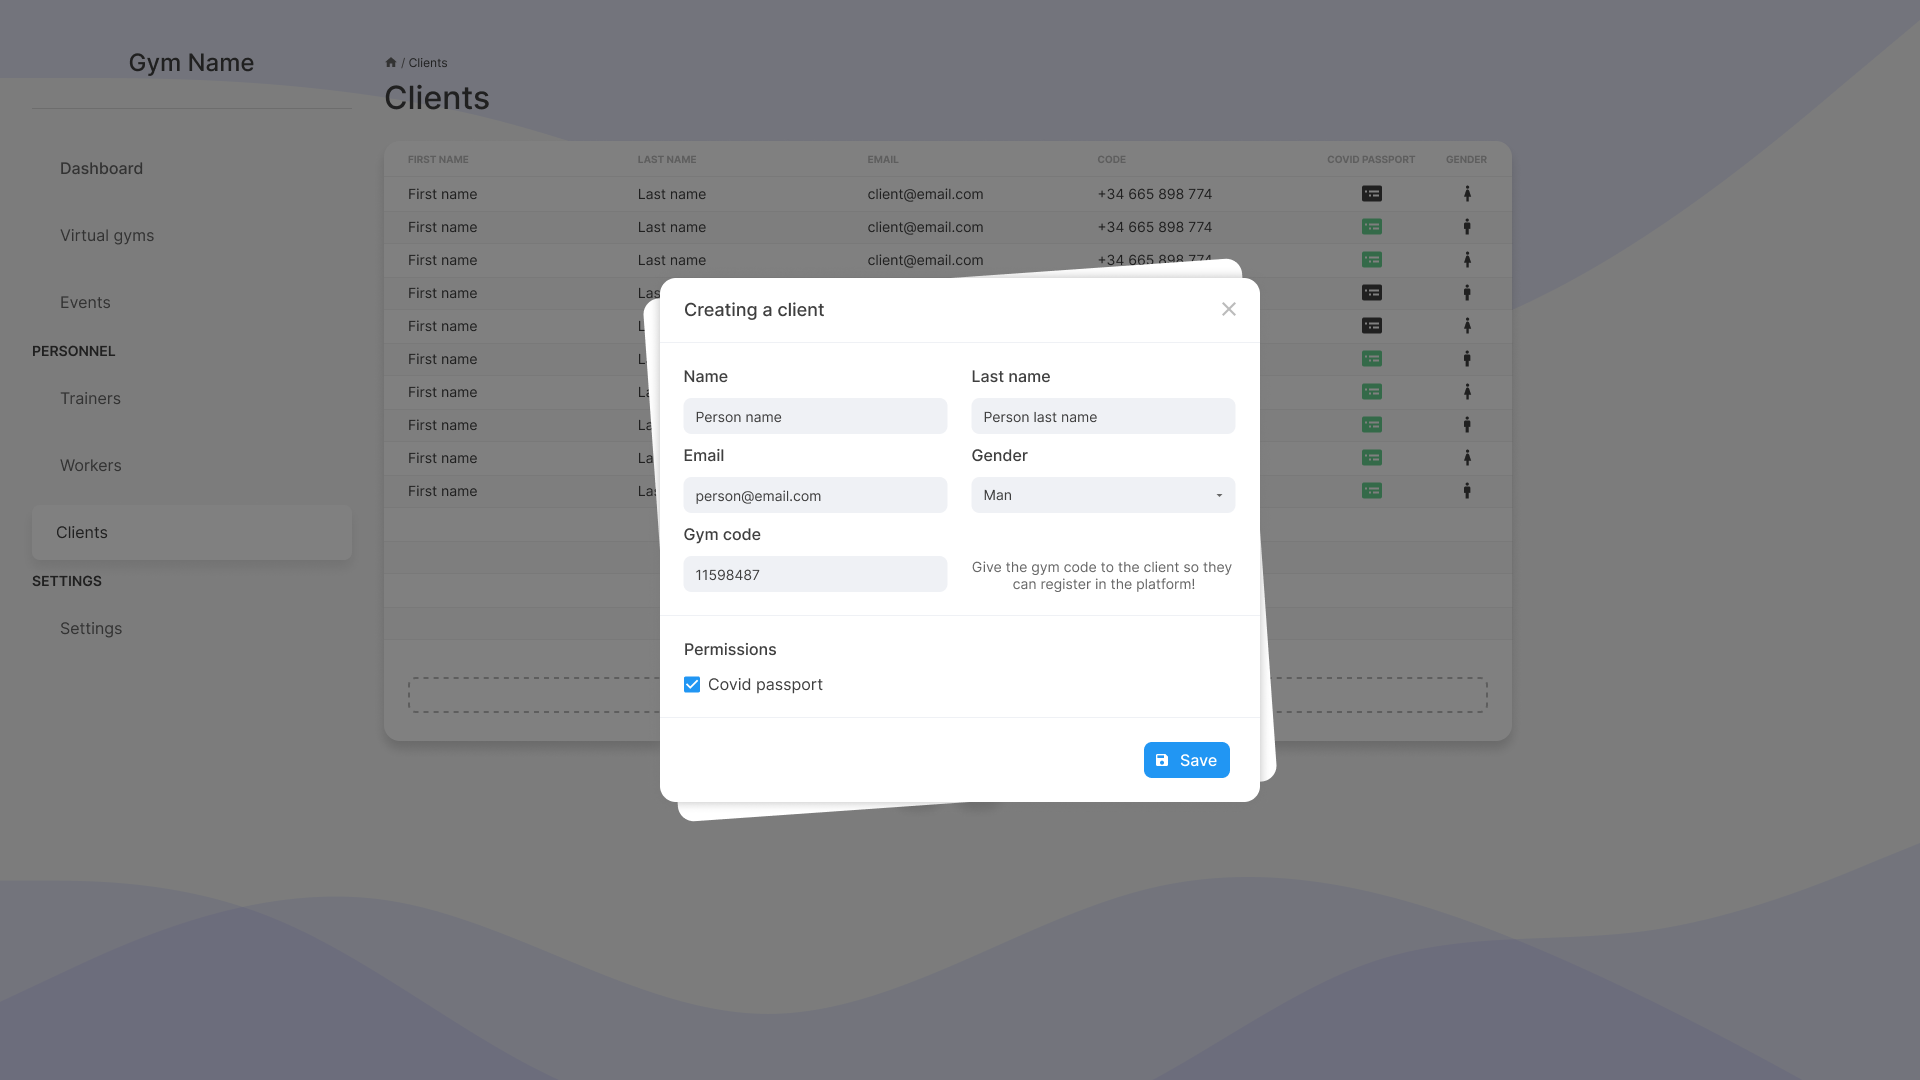
\includegraphics[width=\textwidth]{assets/ui/ClientsCreate.png}
	\caption{Client dialog (create state)}
\end{figure}
\begin{figure}[H]
	\centering
	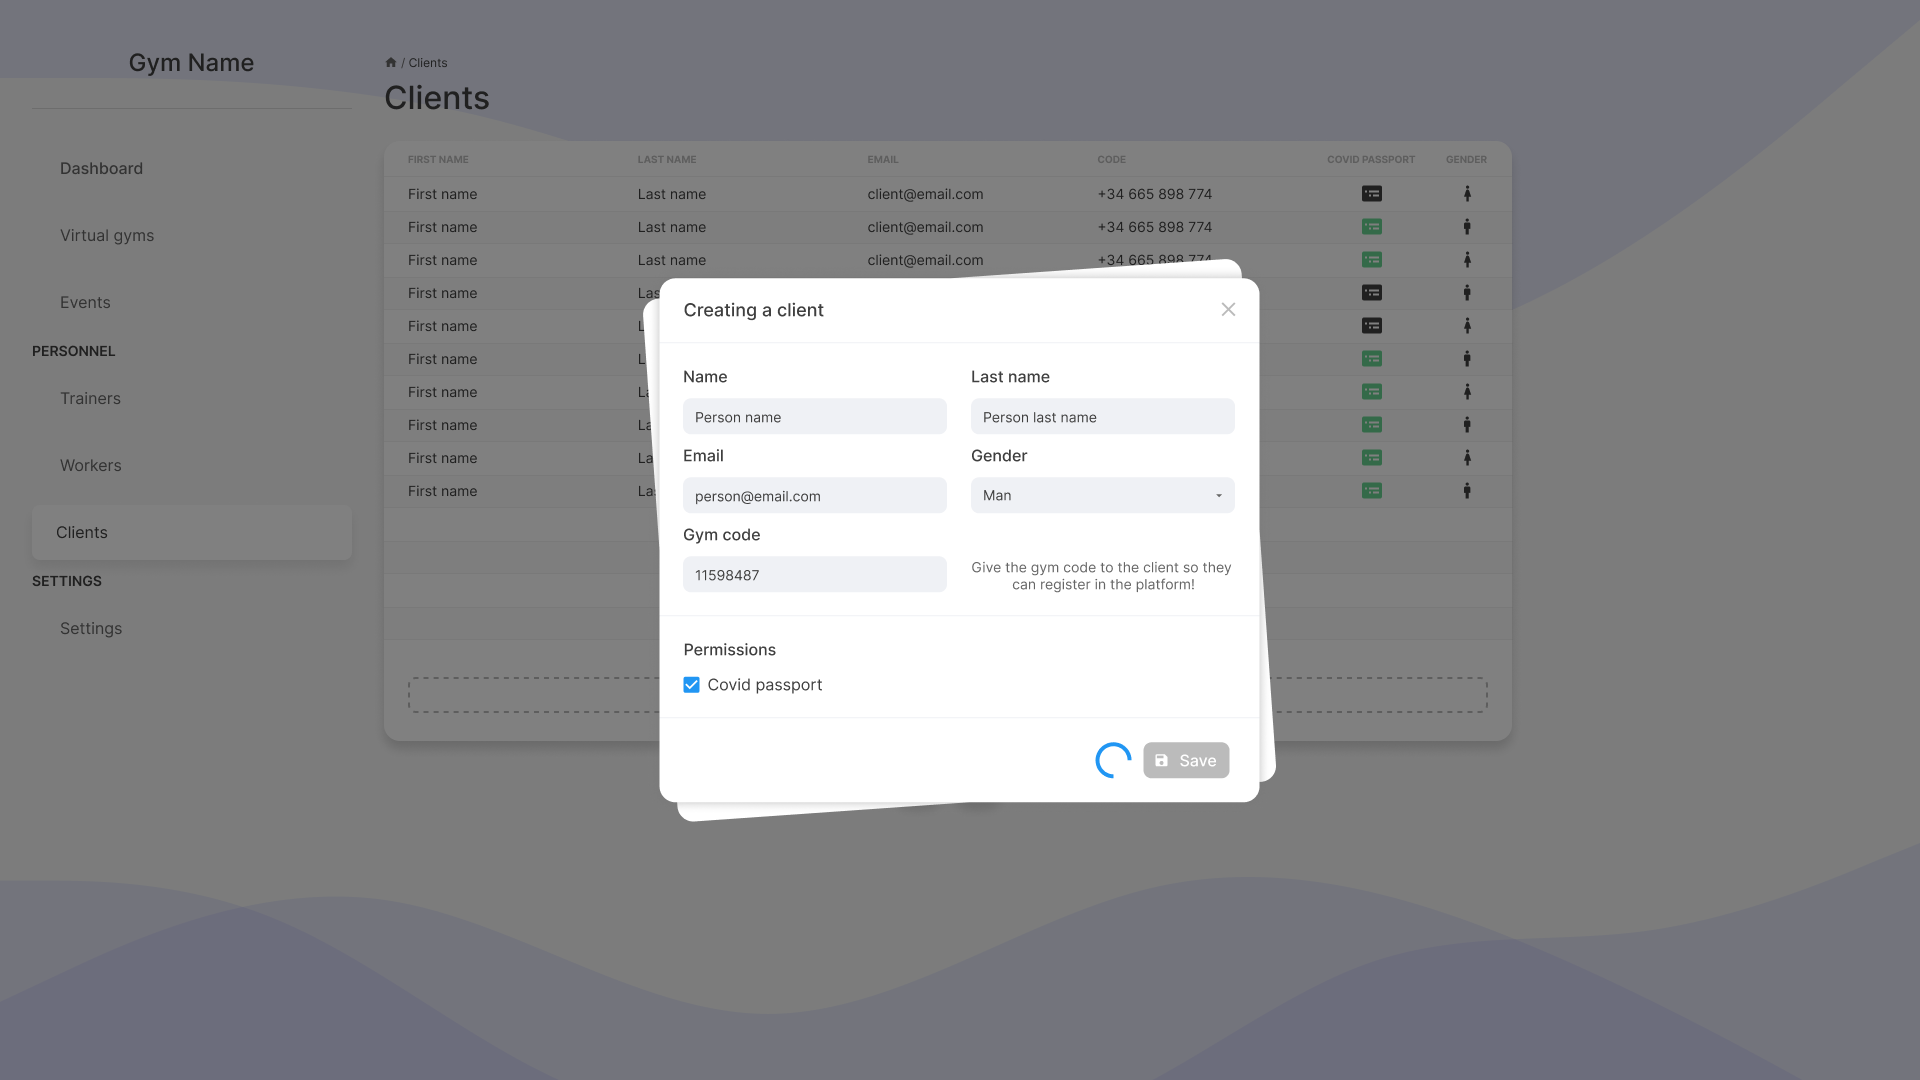
\includegraphics[width=\textwidth]{assets/ui/ClientsCreateLoading.png}
	\caption{Client dialog (create-loading state)}
\end{figure}
\begin{figure}[H]
	\centering
	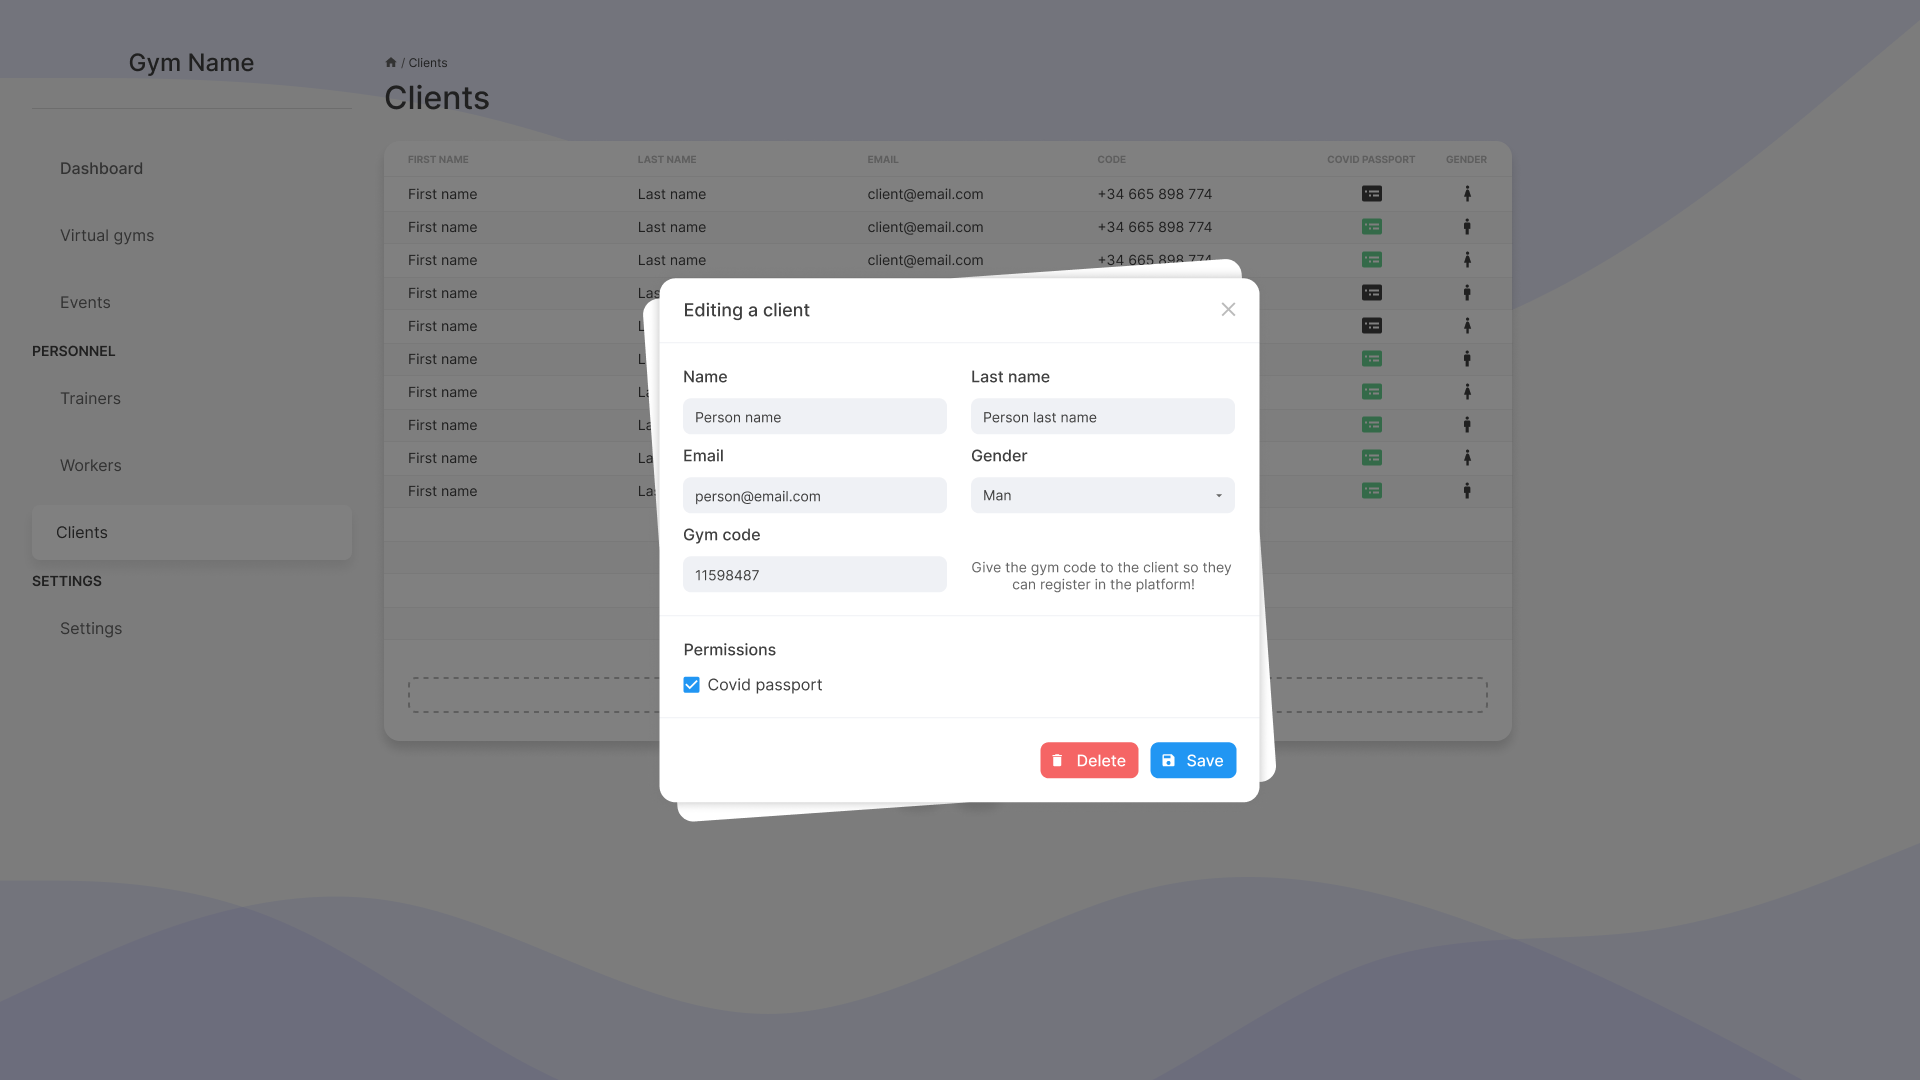
\includegraphics[width=\textwidth]{assets/ui/ClientsEdit.png}
	\caption{Client dialog (edit state)}
\end{figure}
\begin{figure}[H]
	\centering
	\includegraphics[width=\textwidth]{assets/ui/ClientsEditLoading.png}
	\caption{Client dialog (edit-loading state)}
\end{figure}
\begin{figure}[H]
	\centering
	\includegraphics[width=\textwidth]{assets/ui/Owner.png}
	\caption{Settings page, from the owner's view}
\end{figure}
\begin{figure}[H]
	\centering
	\includegraphics[width=\textwidth]{assets/ui/Worker.png}
	\caption{Settings page, from the worker's view}
\end{figure}
\begin{figure}[H]
	\centering
	\includegraphics[width=\textwidth]{assets/ui/Client.png}
	\caption{Settings page, from the client's view}
\end{figure}
% endregion Images
\section{Roadmap}
Once that the tasks required to develop the project have been determined and specified, the time management can be easily structured, using a Gantt's diagram. Such diagram provides an estimated visualisation of the projecte development: visualising the start and finish of each part of the project.
\\[8pt]
Nonetheless, it is still an aproximation. Many things may happen during the development of the project, for instance, a web service that was not expected when plannig the project, yet now is necessary. The tasks that have not been planned, since were difficult to predict, may affect negatively the project schedule, distorting the roadmap. On the contrary, it could happen that some task was overestimated, or may not even be necessary. Such tasks will also affect the roadmap.
\subsection{Gantt's diagram}
Since the number of packages is very large, the diagram has been structure in their parent packages. Therefore, the roadmap only contains the workig packages groups that have been explained in the \emph{\nameref{working-packages}} section. Furthermore, a brief explanation is required, as the diagram does not talk by itself.
\\[8pt]
First, the \emph{Project management} package has a square in the roadmap everytime a part of the project is started. That is because the documentation has to be continually updated, with the new changes in order to keep consistency between the documentation and the project. Secondly, the \emph{Analysis \& Design} group has been divided in two parts. The first part involves the design of the database. This design is a bare initial implementation, as it may change while the project is being developed. The second part is the design of the user interfaces. An important amount of views will be designed, and it would speed up the process if the API application is already implemented, since knowing what data the server will provide, the UI is easier to design. That is why the second part happens after the development of the API application. Third, at the same time the database design is started, the \emph{Development env} group of tasks will take place. The reason behind this decision is due to the fact that the development environment and the database design are related. Fourth, the client side applications will be developed one after the other. The main group, the \emph{Core application} will take most of the amount of time, since it is the most complex. Furthermore, one of the goals of the project is the creation of libraries which allow the reuse of code within the applications. Such abstraction will accelerate and simplify the development of the client and landing applications. Last but not least, there's one group that does not appear in the diagram. Such grup is the \emph{Testing} group. The reason why the group has not been added to the roadmap is beacause the testing of the application it is something that has to be done while the application is being developed. As explained previously, the application has been developed using a TDD methodology, therefore, testing is mandatory.
\newpage
\begin{figure}[H]
	\centering
	\includegraphics[width=0.45\textwidth]{assets/roadmap.png}
	\caption{Chronogram of the development process}
\end{figure}
\end{document}